% vim:ts=4:sw=4
%
% Copyright (c) 2008-2009 solvethis
% Copyright (c) 2010-2014 Casper Ti. Vector
% Public domain.
%
% 使用前请先仔细阅读 pkuthss 和 biblatex-caspervector 的文档,
% 特别是其中的 FAQ 部分和用红色强调的部分。
% 两者可在终端/命令提示符中用
%   texdoc pkuthss
%   texdoc biblatex-caspervector
% 调出。

% 采用了自定义的(包括大小写不同于原文件的)字体文件名,
% 并改动 ctex.cfg 等配置文件的用户请自行加入 nofonts 选项;
% 其它用户不用加入 nofonts 选项,加入之后反而会产生错误。
%
% 图书馆要求电子版论文的目录必须为黑色,
% 且某些教务要求打印版论文的文字部分为纯黑色而非灰度打印,
% 【因此最终打印和提交论文前,请将“colorlinks”改为“nocolorlinks”。】
%\documentclass[UTF8, colorlinks]{pkuthss}
\documentclass[UTF8, nocolorlinks]{pkuthss}

% 使用 biblatex 排版参考文献,并规定其格式。
%
% 如果无法使用 biber,可以把“backend = biber”改为“backend = bibtex”,
% 并改用 bibtex 产生参考文献,详见 pkuthss 的文档。
% 使用 biber 时,请去掉所有的 sorting 选项,否则会出错。
%
% 默认按照引用顺序排序(“sorting = none”),详见 biblatex-caspervector 的文档
% (因为是默认设置所以其实不用写,不过出于完备性的考虑仍然在这里列出)。
% 若需要按照英文文献在前,中文文献在后排序,请设置“sorting = ecnty”;
% 若需要按照中文文献在前,英文文献在后排序,请设置“sorting = centy”。
\usepackage[backend = biber, style = caspervector, utf8, sorting = none]{biblatex}
% 产生 originauth.tex 里的 \square。
\usepackage{amssymb}
\usepackage{morefloats}
\usepackage{lscape}
\usepackage{multirow}
\usepackage{amsmath,bm}
\usepackage{epsf}

\newcommand{\nat}{Nature}
\newcommand{\mnras}{MNRAS}
\newcommand{\apj}{ApJ}
\newcommand{\apjl}{ApJL}
\newcommand{\apjs}{ApJS}
\newcommand{\aap}{A\&A}
\newcommand{\pasa}{Publications of the Astronomical Society of Australia}
\newcommand{\apss}{Ap\&SS}
\newcommand{\araa}{ARAA}
\newcommand{\aj}{Astron. J.}
\newcommand{\aaps}{A\&AS}
\newcommand{\aplett}{Astrophys. Lett.}
\newcommand{\cjaa}{ChJAA}
\newcommand{\aapr}{Astron. Astrophys. Rev.}
\newcommand{\pasj}{Publications of the Astronomical Society of Japan}
\newcommand{\na}{New Astronomy}
\newcommand{\actaa}{Acta Astron.}
\newcommand{\prd}{Phys. Rev. D}

% 设定文档的基本信息。
\pkuthssinfo{
%	cthesisname = {本科生毕业论文}, ethesisname = {Undergraduate Thesis},
	cthesisname = {博士生毕业论文}, ethesisname = {PhD Thesis},
	ctitle = {脉冲星类致密天体的多波段研究}, etitle = {Multi-wavelength Studies of Pular-like Compact Objects},
	cauthor = {代实},
	eauthor = {Shi Dai},
	studentid = {1001110132},
	date = {2015年4月},
	school = {物理学院},
	cmajor = {天体物理}, emajor = {Astrophysics},
	direction = {脉冲星类致密天体},
	cmentor = {徐仁新教授,George Hobbs博士}, ementor = {Prof.\ Renxin Xu, Dr. George Hobbs},
	ckeywords = {脉冲星,射电观测和数据处理,高能天体物理}, ekeywords = {Pulsar, radio observatoin and data analysis, high energy astrophysics}
}
% 导入参考文献数据库(注意不要省略“.bib”)。
\addbibresource{lensing.bib}
\addbibresource{magnetar.bib}
\addbibresource{grb.bib}
\addbibresource{thesis.bib}

% 普通用户可删除此段。
\def\pkuthssffaq{%
%	\emph{\textcolor{red}{pkuthss 文档模版最常见问题:}}
%
%	最终打印和提交论文前,
%	请将 pkuthss 文档类选项中的 %
%	\texttt{colorlinks} 改为 \texttt{nocolorlinks},
%	因为图书馆要求电子版论文的目录必须为黑色,
%	且某些教务要求打印版论文的文字部分为纯黑色而非灰度打印。
%
%	\texttt{\string\cite}、\texttt{\string\parencite} %
%	和 \texttt{\string\supercite} 三个命令分别产生%
%	未格式化的、带方括号的和上标且带方括号的引用标记:%
%	\cite{test-en},\parencite{test-zh}、\supercite{test-en, test-zh}。%
%
%	若要避免章末空白页,请在调用 pkuthss 文档类时加入 \texttt{oneside} 选项。
}

\begin{document}
	% 以下为正文之前的部分。
	\frontmatter

	% 自动生成标题页。
	\maketitle
	% 版权声明。
	% vim:ts=4:sw=4
%
% Copyright (c) 2008-2009 solvethis
% Copyright (c) 2010-2014 Casper Ti. Vector
% All rights reserved.
%
% Redistribution and use in source and binary forms, with or without
% modification, are permitted provided that the following conditions are
% met:
%
% * Redistributions of source code must retain the above copyright notice,
%   this list of conditions and the following disclaimer.
% * Redistributions in binary form must reproduce the above copyright
%   notice, this list of conditions and the following disclaimer in the
%   documentation and/or other materials provided with the distribution.
% * Neither the name of Peking University nor the names of its contributors
%   may be used to endorse or promote products derived from this software
%   without specific prior written permission.
%
% THIS SOFTWARE IS PROVIDED BY THE COPYRIGHT HOLDERS AND CONTRIBUTORS "AS
% IS" AND ANY EXPRESS OR IMPLIED WARRANTIES, INCLUDING, BUT NOT LIMITED TO,
% THE IMPLIED WARRANTIES OF MERCHANTABILITY AND FITNESS FOR A PARTICULAR
% PURPOSE ARE DISCLAIMED. IN NO EVENT SHALL THE COPYRIGHT HOLDER OR
% CONTRIBUTORS BE LIABLE FOR ANY DIRECT, INDIRECT, INCIDENTAL, SPECIAL,
% EXEMPLARY, OR CONSEQUENTIAL DAMAGES (INCLUDING, BUT NOT LIMITED TO,
% PROCUREMENT OF SUBSTITUTE GOODS OR SERVICES; LOSS OF USE, DATA, OR
% PROFITS; OR BUSINESS INTERRUPTION) HOWEVER CAUSED AND ON ANY THEORY OF
% LIABILITY, WHETHER IN CONTRACT, STRICT LIABILITY, OR TORT (INCLUDING
% NEGLIGENCE OR OTHERWISE) ARISING IN ANY WAY OUT OF THE USE OF THIS
% SOFTWARE, EVEN IF ADVISED OF THE POSSIBILITY OF SUCH DAMAGE.

\chapter*{版权声明}
{
	\zihao{3}\linespread{1.5}\selectfont

	任何收存和保管本论文各种版本的单位和个人,
	未经本论文作者同意,不得将本论文转借他人,
	亦不得随意复制、抄录、拍照或以任何方式传播。
	否则一旦引起有碍作者著作权之问题,将可能承担法律责任。
	\par
	% 若需排版二维码,请将二维码图片重命名为“barcode”,
	% 转为合适的图片格式,并放在当前目录下,然后去掉下面 3 行的注释。
	%\vfill\noindent
	%\includegraphics[height = 5em]{barcode}
	%\par
}


	% 中英文摘要。
	% vim:ts=4:sw=4
% Copyright (c) 2014 Casper Ti. Vector
% Public domain.

\begin{cabstract}

脉冲星类致密天体是宇宙中可直接观测的最致密的天体。它们不仅有丰富的多波段的观测现象,
还对于基础物理的研究有重要意义。除了可以用于检验引力理论,脉冲星类致密天体的结构
和状态方程直接反应了致密物质的物态、强相互作用以及QCD相变的本质。在我攻读博士学位
期间,我在北京大学和CSIRO Astronomy and Space Science展开了对于脉冲星类致密天体的
多波段的研究。

我的研究主要部分是关于射电脉冲星,尤其是射电脉冲星的高精度测时和脉冲星测时阵列(pulsar timing array, PTA)。
使用Parkes Pulsar Timing Array的数据,我们研究了24颗毫秒脉冲星的多波段的脉冲偏振
轮廓。为了理解多种与频率相关的效应对脉冲星测时精度的影响,我们开发了新的脉冲星
模拟和测时软件。我们还讨论了五百米口径球面望远镜(Five-hundred-meter Aperture Spherical Telescope)
对于未来脉冲星测时阵列研究的贡献。

为了寻找新的测量脉冲星质量的方法,我研究了由中子星和射电脉冲星导致的微引力透镜
事件的性质。我们讨论了未来的大型望远镜发现由射电脉冲星导致的astrometric microlensing
事件的可能性。我们的结果显示,通过astrometric microlensing现象,我们可以较精确
地测量脉冲星的质量。假设脉冲星的距离可以通过射电观测限制,那么脉冲星的质量可以
测量精确到约10\%。在X射线波段,我们研究了反常X射电脉冲星和软伽马射线重复包
的硬X射电谱。
	\pkuthssffaq
\end{cabstract}

\begin{eabstract}

Pulsar-like compact objects as the densest observable objects in the Universe, are not only
important in understanding diverse astrophysical phenomena, but also significant in fundamental
physics. Besides the physics of gravity, the answer to the question that whether pulsar-like
compact stars are neutron stars or quark stars would have profound implications on the physics
of condensed matter, the nature of strong interaction as well as QCD phase transition. During 
my PhD study at Peking University and CSIRO Astronomy and Space Science, I carried out multi-wavelength 
researches on pulsar-like compact objects. 

The main part of my study is focused on radio pulsars, especially on high precision timing of 
radio pulsars and pulsar timing arrays (PTAs). Using the Parkes Pulsar Timing Array data 
sets, we studied the multi-frequency polarization pulse profiles of 24 millisecond pulsars. We
developed new simulation and timing software packages to investigate various frequency-dependent 
effects on the precision of pulsar timing. We also studied how the Five-hundred-meter Aperture 
Spherical Telescope can contribute to the PTA studies. 

To find new ways to measure pulsar masses, I investigate properties of Galactic microlensing 
events caused by neutron stars and pulsars. We describe a possible study of astrometric microlensing 
events using radio pulsars that are likely to be discovered by future large telescopes. We show 
that such a study could lead to precise measurements of pulsar masses. For instance, if a pulsar 
distance could be constrained through radio observations, then its mass would be determined with 
a precision of $\sim$10\%. In the X-ray band, we studied the hard X-ray spectrum of AXPs and SGRs 
using XMM-Newton, Suzaku and INTEGRAL data. 

\end{eabstract}


	% 自动生成目录。
	\tableofcontents

	% 以下为正文。
	\mainmatter

	% 序言。
	% vim:ts=4:sw=4
% Copyright (c) 2014 Casper Ti. Vector
% Public domain.

\specialchap{序言}

脉冲星类致密天体是快速旋转的、高度磁化的中子星。它们最重要的特征之一
是从伽马射线波段到射电波段的多波段脉冲辐射。由于中子星是宇宙中
最致密的天体之一,脉冲星类致密天体极为丰富的多波段现象使它们成为
研究致密物质的状态和引力本质的独一无二的天体物理实验室。而射电脉
冲星稳定的脉冲信号又使它们成为强有力的工具,被广泛用于研究星际介质、
探测引力波以及导航等。

射电脉冲星于1967年被Jocelyn Bell-Burnell和Antony Hewish等首次发现\supercite{hbp+68},
Hewish因这一发现而被授予了1974年的诺贝尔物理学奖。人们很快意识到,脉冲星
极短的自转周期意味着致密的物态,而脉冲信号来自强磁场中的辐射过程,
因而这类天体将向我们展现多种多样的极端现象。于是自发现以来人们一直
在使用多个大型射电望远镜以及利用多波段的观测搜寻脉冲星。目前为止我们
已经发现了2300多颗脉冲星类致密天体,其中大部分是射电脉冲星。对
脉冲星类致密天体的多波段研究也取得了丰富的成果。Russell Hulse和Joseph Taylor
在1975年发现了首个双中子星系统B1913$+$16\supercite{ht75}。
这个双星系统的轨道周期是7.75小时,并且由于引力波辐射损失轨道
能量,预计将在200兆年后并合。通过测量轨道周期由于引力波辐射损失
能量导致的缩减,Hulse和Taylor首次给出了引力波存在的间接证据,并因此
获得了1993年的诺贝尔物理学奖。首个脉冲星行星系统B1257$+$12在1990
年由Alexander Wolszczan和Dale Frail使用Arecibo望远镜发现\supercite{wf92}。
这个系统包含了两颗地球质量的行星和一颗月亮质量的行星\supercite{wol94},
更重要的是这是第一次在太阳系外发现包含行星的系统。在球状
星团中的脉冲星由Andrew Lyne及其合作者首次发现\supercite{lbm+87}。在这
之后人们已经在球状星团中发现了几十颗脉冲星,这些发现使我们第一次
探测到了球状星团中的电离气体\supercite{fkl+01}。

除了射电脉冲星,使用多个X射线望远镜和伽马射线望远镜,人们还发现
了很多种脉冲星类致密天体,包括X射线脉冲星(X-ray pulsar)、中心致密
天体(compact central objects,CCO)、暗热中子星(dim thermal neutron star,DTN)、
反常X射线脉冲星(anomalous X-ray pulsar,AXP)、软伽马射线
重复爆(soft gamma-ray repeater,SGR)以及伽马射线脉冲星(gamma-ray pulsar)。
这些天体在X射线和伽马射线波段的辐射对于我们理解双星系统的演化、
脉冲星的辐射机制等有重要意义,而一些极端的爆发现象更是对于
脉冲星类致密天体的物态提出了挑战\supercite{m08}。

我在博士期间对多种脉冲星类致密天体开展了多波段的研究。在射电
波段,我们主要研究了毫秒脉冲星的多波段脉冲偏振轮廓、脉冲星的高
精度测时以及脉冲星测时阵列;在光学波段,我们的工作主要是关于使
用微引力透镜的方法测量脉冲星的质量;在X射线波段,我们研究了反常
X射电脉冲星和软伽马射线重复爆的硬X射线辐射特征。在介绍我博士生
阶段的具体研究工作之前,我先简要评述脉冲星的科学和应用研究,以及
未来中国脉冲星研究的前景。

\section{脉冲星的科学研究}

尽管脉冲星已经被发现近半个世纪了,并且人们开发和使用了大量的设备
和方法来对脉冲星类致密天体进行多波段研究,但是我们对于脉冲星的
理解还是非常有限的。我们仍然不清楚脉冲星的结构和内部的物态,
也不清楚脉冲星磁层的结构和辐射机制。我们仍然需要回答,脉冲星
到底是中子星还是夸克星?脉冲星的磁场和电场的结构如何?磁层
中的等离子体密度是多少?相干射电辐射是如何产生的?高能辐射是从磁层
的什么位置以及如何产生的?目前我们还不知道上面任何一个
问题的确切答案,而这些问题的答案将直接为我们揭示致密物质的
物态和在极端条件下的等离子体物理。

另一方面,脉冲星极为稳定的自转以及辐射的脉冲信号使其成为研
究多种天体物理现象和基础物理问题的强大工具。虽然我们仍然不清楚
脉冲星内部的结构和物态,也不能完全理解多波段辐射的机制,
但是这并不影响我们使用脉冲星的稳定的周期性信号。特别是
通过射电脉冲星的高精度测时,我们可以研究双星系统的动力学性质、
星际介质的性质、银河系的引力场和磁场,还可以检验引力理论
和探测引力波辐射。使用脉冲星还可以在未来建立独立的时间标
准和进行星际导航。

要提取脉冲星脉冲信号中的信息,我们首先需要测量脉冲的
到达时间(pulse time of arrival,ToA),这个过程被称为
脉冲星测时。在射电波段,脉冲星的射电信号被射电望远镜
接收、放大、采样以及数字化。我们消除星际介质导致的色散
延迟,并在频率和时间上将观测数据叠加得到高信噪比的脉冲轮廓。
通过将脉冲轮廓与一个脉冲轮廓模板进行相关,我们得到脉冲
轮廓的相位移动,并最后转化为脉冲的到达时间。这样得到的
脉冲到达时间是在观测者参考系下的,我们需要将其转换到太阳系
质心参考系,并且要考虑太阳以及行星对脉冲到达时间的影响。
得到太阳系质心处的脉冲到达时间后,我们使用一个脉冲星
自转减慢、双星轨道和天体测量参数的模型来拟合脉冲到达时间,
并且将观测得到的到达时间跟最佳拟合模型之间的差别称为测时残差。
不正确或者不完备的脉冲星模型将导致测时残差中出现系统性的
偏离,但是同时也给我们提供了研究脉冲星参数以及信号在
星际空间中传播过程的工具。例如我们可以通过脉冲星测时发现
脉冲星的行星、测量色散延迟随时间的变化等等。

多颗测时精度比较高的射电脉冲星可以组成脉冲星测时阵列(pulsar 
timing arrays,PTAs)。脉冲星测时阵列中的脉冲星的测时
残差的相关性可以帮助我们研究多种现象。脉冲星测时的
本征不稳定性、脉冲周期的跳变以及星际介质的变化将导致各个
脉冲星之间不相关的测时残差;地面时间标准的偏差将导致
各个脉冲星之间完全相同的测时残差偏离;太阳系历书的误差
致使各个脉冲星的测时残差偏离与它们的位置有关(偶极关联);
而由引力波导致的测时残差偏离的幅度和相位依赖于脉冲星和地球
连线的夹角(四极关联)。脉冲星测时阵列扩展了脉冲星测时的应用,发展了新的
探测引力波辐射的方法,也提供了研究太阳系的动力学、
脉冲星时间标准的途径。要实现脉冲星测时阵列的科学目标,
我们需要高精度的测时,目前只能在毫秒脉冲星上实现。
毫秒脉冲星有很短的自转周期,同时也有高度稳定的脉冲轮廓,
从而使测时的精度远高于常规脉冲星,达到几百纳秒的量级。
第一个脉冲星测时阵列,Parkes Pulsar Timing Array (PPTA)
于2004年使用Parkes望远镜建立\supercite{Manchester13}。
欧洲脉冲星测时阵列(European Pulsar Timing Array,EPTA)\supercite{fvr+10}
使用了Jodrell Bank、Effelsberg、Nancay以及Sardinia的望
远镜建立。北美纳赫兹引力波望远镜(North American Nanohertz Observatory of Gravitational Waves,
NANOGrav)\supercite{jfl+09}主要使用Green Bank和Arecibo
望远镜。这三个脉冲星测时阵列又一起组成了国际脉冲星测时
阵列(International Pulsar Timing Array,IPTA),总共
包含了约40颗测试精度较高的毫秒脉冲星。国际脉冲星测时阵列
的数据最有希望在不远的将来首次探测到低频的引力波辐射。

\subsection{脉冲星的结构和物态}

脉冲星是在超新星爆发过程中产生的致密天体。假设质量是1.4倍太阳
质量,半径是10公里,那么脉冲星的密度将高达6.7$\times$10$^{14}$\,g/cm$^{-3}$,
甚至高于核物质密度2.8$\times$10$^{14}$\,g/cm$^{-3}$。在如此高的
密度下,物质的物态目前是不清楚的,极有可能出现夸克物质、玻色子
凝聚和奇异物质。Witten在1984年的工作中猜想\supercite{wit84},
奇异夸克物质可能是物质的基态,即在零压下有比铁更低的能量。根
据这一猜想,当物质的密度足够高时可能诱发从常规物质向奇异夸克物
质的相变,从而将整个星体相变为奇异夸克星。这样的奇异夸克星将是
自束缚的,而不是像常规中子星那样被引力束缚。

传统的中子星模型认为脉冲星主要是由中子组成的。在中子星的表面
有一个固态的壳层,大概储存了中子星2\%的转动惯量。而在壳层之下,
是液态的内核。从壳层到内部,中子星
密度逐渐升高,跨越大概九个数量级。接近中子星表面,固态的壳层
主要由铁核和简并的电子组成,密度约为10$^{6}$\,g/cm$^{-3}$。
向中子星内部移动,密度逐渐升高直到质子和电子开始结合形成中子,
从而形成富中子核的内壳层。在达到“中子滴”密度(4$\times$10$^{11}$\,g/cm$^{-3}$)
的半径之后(大约中子星表面之下几百米),中子所占的比例快速
提高。在密度超过2$\times$10$^{14}$\,g/cm$^{-3}$之后,中子星
将主要由超流态的中子组成,同时混合有大概5\%的超导的电子和质子。

随着人们意识到强子是由更基本的夸克组成的,以及夸克之间的色
相互作用的渐近自由特性,奇异夸克物质的稳定性及其天体物理后果
开始引起人们的关注\supercite{wit84}。1986年Haensel等人\supercite{hzs86}
和Alcock等人\supercite{afo86}等人基于游离夸克模型,首次计算
给出了奇异夸克星的结构并讨论了这样的天体的观测表现。然而,
我们知道脉冲星的温度往往只有几个keV,因此是属于低能量子
色动力学(QCD)的范畴,非微扰QCD还有很大挑战。如果在几倍
核物质密度下夸克之间的色相互作用还比较强,致密物质中有可能
出现多夸克态,形成由u、d、s三味夸克组成的夸克集团。类似
于核子,夸克集团间可能还存在着剩余的短程排斥和远程吸引
的强相互作用。而当温度足够低时,夸克集团将像经典粒子那样
固化形成固态的夸克集团物质。

传统中子星模型和固态夸克集团星模型之间的差别主要体现在如下两个方面。
\begin{itemize}
\item 脉冲星的表面:传统中子星表面上的原子核和电子是被引力束缚的,
而固态夸克集团星表面的夸克是强相互作用束缚的,电子则是被强电磁力
束缚的。这种差别首先将导致不同的质量和半径的关系。对于引力束缚的
中子星,因为质量越大引力越强,半径随着质量的增加而减小;对于自束缚
的固态夸克集团星,表面密度非零,未接近极限质量之前半径随着质量的
增加而增加。特别是对于低质量夸克集团星,引力作用可以忽略,于是
质量正比于半径的三次方。其次,固态夸克集团星的强束缚表面意味着
可以存在裸的星体表面,而传统中子星表面通常被认为存在大气。裸的星体表面可以
自然地解释我们在无磁层活动的脉冲星的X射电波段的热辐射谱没有
观测到原子谱线。同时强束缚的表面还可以解释射电脉冲星的子脉冲
偏移现象以及超爱丁顿光度的爆发现象等。
\item 脉冲星的结构:传统中子星模型和固态夸克集团星模型预言了
不同的星体内部密度和压强的关系,即状态方程。而状态方程的软硬
直接决定了脉冲星的极限质量。另一方面,固态夸克集团星整体都由
夸克集团构成,因而具有整体的刚性,而传统脉冲星由于内部的超流
结构不具备刚性。首先,与传统夸克星模型不同,固态夸克集团星内部
的夸克集团物质质量比较大因而是非相对论性的,同时有短程的排斥
相互作用,于是导致了更硬的状态方程。更硬的状态方程意味着更大的极
限质量。目前测量到的大于两个太阳质量的脉冲星就是对较硬的物态的支持。其次,
具有整体刚性的固态夸克集团星在自由转动和力矩作用下都更容易
产生进动,这可以自然地解释在一些脉冲星中观测到的进动。
\end{itemize}

尽管不同的脉冲星模型给出了不同的观测预言,但是现实的观测往往
是非常复杂的,很难提供确凿的证据来区分不同的模型。自束缚的星体
与引力束缚的星体往往有相似的半径、转动惯量以及中微子发射率和
透明度,而脉冲星的磁层和周围环境又极为复杂,因此很难通过光子
或者中微子观测,甚至射电脉冲星的测时来区分内部结构和物态。
最有希望的区分不同脉冲星模型和状态方程的途径是测量脉冲星的
质量和半径,特别是脉冲星极大和极小质量的测量。传统中子星模型
可以支持的最大质量是三倍太阳质量,这是基于广义相对论的结果
并且是由状态方程的软硬决定的\supercite{rr74}。但当在高于核物质
密度时引入超子自由度后,状态方程将显著变软,意味着更低的极限
质量,通常难以高于两倍太阳质量。而对于固态夸克集团星,由于
夸克集团是非相对论性的且有近程排斥相互作用,所以状态方程远比
传统中子星模型硬。
在很宽的参数范围内,固态夸克集团星的极限质量可以高于两倍
太阳质量,甚至可以高于三倍太阳质量\supercite{lgx13}。因此,
如果发现极大质量的脉冲星,那么我们将能极强地限制状态方程,
从而促进我们对致密物质物态的理解;而如果我们发现极小质量的
脉冲星,那么将说明脉冲星是自束缚而不是引力束缚的。

脉冲星的质量和半径的测量都是极有挑战性的。目前对脉冲星半径
的估测主要是通过脉冲星冷却过程中的热辐射、脉冲星在爆发过程
(包括热核爆炸、软伽马射线重复爆的巨爆发等)中的性质以及脉
冲星的周期跳变(glitch)现象等等。这些估测都还很不精确,很难
有效地限制脉冲星模型。脉冲星质量的测量要精确得多,这主要
得益于高精度的射电脉冲星测时。通过长期监测那些edge on的双星
系统中的射电脉冲星,我们可以精确地测量Shapiro延迟效应,从而
得到伴星质量,然后再根据双星系统参数测算出脉冲星质量。近年来
通过高精度的测时,人们已经测量到了两颗超过两倍太阳质量的
脉冲星\supercite{Anton,Demorest}。这两颗大质量脉冲星已经排除
了很多传统中子星模型和传统夸克星模型,并对于脉冲星的状态方程
给出了很强的限制\supercite{Ozel2010,Lai2011}。

但是目前能精确测量质量的脉冲星都是在双星系统中,孤立脉冲星
的质量测量还是一个挑战。而孤立脉冲星由于不在双星系统中,
可能有不同的演化过程,并且没有吸积的过程,因此可能有不同
的质量分布范围,更可能出现超大质量或者极小质量的脉冲星。一种
可能的测量孤立脉冲星质量的方法是微引力透镜效应\supercite{Dai,dsl+15},
我们将在后面的章节中具体讨论。

\subsection{脉冲星的磁层和辐射机制}

脉冲星可以看作转动的、高度磁化的、高导电率的球体。星体内部的磁场,$\mathbf{B}$,
将导致一个电场,$(\mathbf{\Omega\times r)\times B}$。对于
一个导体,磁场导致的电场将被内部电子重新分布导致的电场,$\mathbf{E}$,
平衡,于是在星体内部任意一点,$\mathbf{r}$,电场力平衡给出
\begin{equation}
\mathbf{E}+\frac{1}{c}\mathbf{(\Omega\times r)\times B}=0.
\end{equation}
如果星体外部是真空,星体表面的电子将导致一个外部的四极电场,
\begin{equation}
\Phi(r,\theta)=\frac{B_{\rm{S}}\Omega R^{5}}{6cr^{3}}(3\cos^{2}{\theta}-1),
\end{equation}
其中$(r,\theta)$是以星体中心为原点的极坐标系,$B_{\rm{S}}$是
星体表面磁场强度,$R$是星体半径。在星体表面,平行于磁场
方向的电场强度是
\begin{equation}
E_{\parallel}=\frac{\mathbf{E\cdot B}}{B}\arrowvert_{r=R}=-\frac{\Omega B_{\rm{S}}R}{c}\cos^{3}{\theta}.
\end{equation}
使用脉冲星的典型参数进行估算,这个电场导致的电场力将远远超过
星体表面的重力。因此在传统的中子星模型下,中子星表面的
粒子将被这个强电场拉出,在中子星周围形成等离子体。
我们把脉冲星周围由磁场主导、等离子体填充的区域称作脉冲星的磁层。

脉冲星磁层中的带电粒子在电场作用下也将重新分布,并且屏蔽
电场。根据电场力的平衡,在磁极处($r=R,\theta=0$),带电粒子
数密度,$n=\rho_{\rm{e}}/e$,可以计算得到
\begin{equation}
n_{\rm{GJ}}=\frac{\Omega B_{\rm{S}}}{2\pi ce}\simeq 7\times10^{10}\,\rm{cm^{-3}}\,(\frac{P}{s})^{-1/2}(\frac{\dot{P}}{10^{-15}})^{1/2}.
\end{equation}
这一电子密度是由Goldreich和Julian在假设脉冲星自转轴和磁轴
平行的情况下首次计算得到的\supercite{gj69},被称为Goldreich-Julian密度。

在脉冲星电磁场的作用下,磁层中的等离子体随着脉冲星共转。
然而,等离子体的共转速度不能超过光速,于是在某个极限距离
之后等离子体将不再随脉冲星共转。这个极限距离由等离子体的
共转速度等于光速定义,并且给出了一个假想的光速圆柱,半径为
\begin{equation}
R_{\rm{LC}}=\frac{c}{\Omega}\simeq 4.77\times10^{4}\,\rm{km}\,(\frac{P}{s}).
\end{equation}
光速圆柱将偶极磁力线分为了两类:1) 在光速圆柱内
闭合的磁力线(closed field lines);2) 开放的磁力线(open field lines)。
开放磁力线定义了脉冲星的极冠区域(polar cap)。极冠区域以
磁极为中心,它的边界($R,\theta_{\rm{p}}$)由最后
开放磁力线定义。最后开放磁力线是与光速圆柱相切的磁力线,
对于偶极磁场,$\sin^{2}{\theta}/r$是常数,于是我们得到
等式
\begin{equation}
\frac{\sin^{2}{\theta}}{r}=\frac{1}{R_{\rm{LC}}}=\frac{\sin^{2}{\theta_{\rm{p}}}}{R}.
\end{equation}
在脉冲星表面(取$R=10$\,km),极冠区的半径,$R_{\rm{p}}$,可以
估算为
\begin{equation}
R_{\rm{p}}\simeq R\sin{\theta{\rm{p}}}=150\,\rm{m}\,(\frac{P}{s})^{-1/2}.
\end{equation}

开放磁力线区域提供了射电脉冲辐射产生的通道。经典的射电辐射
模型认为磁层中的带电粒子以小集团的形式沿着磁力线运动,产生
曲率辐射。带电粒子集团的尺度不超过辐射波长的一半,其中的带电粒子
以相同的相位辐射,而辐射的能量是单个粒子辐射能量的粒子数目
的平方倍\supercite{kom70,rs75}。然而,曲率辐射的效率是比较
低的,而且人们的研究显示带电粒子集团很难在磁层中快速
形成,并且也无法在足够长的时间内保持集团形式\supercite{mel92}。
人们因此提出了基于相对论性等离子体的辐射机制,这种模型往往需要
等离子体的不稳定性。除了等离子体的不稳定不能很快地扩大这个
问题外,在这样的模型下等离子体湍动产生的能量也很难被传导
出去。人们提出了多种非线性机制尝试将等离子体湍动的能量
转化为某种模式的波,然后向外转移\supercite{mel92}。另外,
脉泽机制也被尝试用于解释脉冲星的射电辐射\supercite{mel89}。

到目前为止,脉冲星射电辐射的机制还不清楚。任何一种模型都
需要解释脉冲星射电辐射的高偏振度和相干性,同时还要理解在
跨越四个量级的自转周期和六个量级的磁场强度的多种情形下多种
观测特征,而且这样的辐射机制需要在很宽的频率范围内有效
($\sim$100\,MHz到100\,GHz)。

与射电辐射机制一样不清楚的是脉冲星辐射束的结构。在曲率辐射
机制下,带电粒子沿着开放磁力线运动,而辐射的能量随着磁力线
曲率的增大而增大。因此,我们期待最外开放磁力线上的辐射最强,
而往辐射束中心移动辐射强度逐渐降低,并在辐射束中心形成一个
空洞。当我们观测时,随着视线扫过辐射束我们将观测到一个有
双峰结构的脉冲轮廓,峰对应着辐射束的边沿,即最外开放磁力线。
然而我们实际观测到的脉冲星脉冲轮廓是极为多样和复杂的,有的
脉冲星的脉冲轮廓只有一个成分,而一些有多个脉冲成分。为了
解释观测现象,人们发展了多种辐射束的结构模型。Backer 1976\supercite{bac76}
提出了cone模型,认为沿着磁轴有一个额外的辐射束,被称为
中心成分(core component)。对cone模型更进一步的改进是
猜测辐射束中有多个cone结构,而中心是一个core成分\supercite{os76,os77,Rankin93,gks93},
于是多个脉冲成分的脉冲轮廓可以被解释。另一种模型认为脉冲星
的辐射束是由随即分布的离散的辐射区域(patch)填充的,并且
只有在开放磁力线区域的辐射斑是活跃的\supercite{Lyne88}。
混合了cone和patch的模型也被提出,Karastergiou \& Johnston (2007)\supercite{Kara07}
认为cone结构沿着靠近极冠边缘的磁力线分布在很宽的高度范围内,
而活跃的辐射区域是在cone结构之间随即分布的。在这种模型下,
年老脉冲星的脉冲轮廓比年轻脉冲星复杂的现象可以得到解释。

人们尝试了多种途径来检验不同的辐射束模型。Cone模型预言
子脉冲和脉冲成分的相位随频率有微弱的演化,而patch模型
则预言没有演化\supercite{gk96,kg02}。Gil \& Krawczyk (1996)\supercite{gk96}
的工作发现观测事实支持cone模型,而Kijak \& Gil (2002)\supercite{kg02}
进一步的工作显示多个cone的模型更符合观测现象,包括脉冲轮廓
的opening angle的双峰分布现象以及单峰和双峰脉冲轮廓更大
的impact angle。为了研究脉冲星辐射束的二维图像,Han \& Manchester (2001)\supercite{Han01}
对87颗有多个脉冲成分的正常脉冲星进行分析,发现除了靠近
辐射束中心的位置强度有所增加,在辐射束的其他位置强度没有明显
的cone结构,从而支持了patch模型。在双星系统中发现的脉冲星的
进动现象使我们有机会扫描探测辐射束的不同部分,从而研究
它的结构。目前,人们已经对六颗有进动的脉冲星PSRs J1913$+$16,
J1534$+$12,J1141$-$6545,J1906$+$0746,J0737$-$3039A和
J0737$-$3039B进行了辐射束的研究\supercite{kra12},发现辐射束中没有明显
的cone结构的证据,但是看到辐射束中有部分区域被照亮,
这些结果明显支持patch模型。最近,Wang et al. (2014)\supercite{Wang14}
讨论了基于宽波段相干辐射的fan beam模型,从不同的角度
解释脉冲轮廓的成分及其随频率的演化。

对于脉冲星辐射机制和磁层结构的研究直接与强磁场下的等离子体
物理相关,同时也有助于我们理解磁层当中的不稳定性,从而
促进脉冲星测试精度的提高。目前已有的脉冲星辐射和磁层模型
还远不能解释我们观测到的所有现象,我们需要更高精度、更高信
噪比的观测。在后面的章节中我们将详细介绍与毫秒脉冲星的
脉冲偏振轮廓相关的工作。

\subsection{银河系的结构和星际介质的研究}

脉冲星在银河系中的分布范围很广,考虑到脉冲星比较大的自行,
更是有可能分布在银河系的任何区域。于是通过对射电脉冲星的
多波段偏振观测,我们可以利用射电脉冲星研究银河系的结构和
星际介质的性质。

射电脉冲星的色散延迟直接反应的是自由电子在视线方向上的
积分柱密度。如果银河系的自由电子分布是已知的,那么我们
可以通过色散测量(dispersion measure,DM)估算脉冲星的
距离。实际上,银河系的自由电子分布是不清楚的,可是如果
脉冲星的距离可以通过其他方式独立的测量,比如通过视察和
中性氢吸收,那么我们可以使用这些脉冲星的色散测量来研究
自由电子的分布\supercite{cordes}。

另一方面,脉冲星的射电脉冲辐射是高度线偏振的。于是
射电脉冲信号在银河系的磁场中传播将会受到法拉第旋转效应的
影响,即线偏振位置角会产生正比于视线方向的磁场强度和电子密度的
旋转。通过测量大量的射电脉冲星的法拉第旋转效应,我们
可以还原银河系的磁场的大尺度结构。Han et al. (2006)\supercite{hml+06}
给出了223颗脉冲星的法拉第旋转测量,并结合之前的测量,
展示了银河系旋臂中逆时针方向的磁场。

脉冲星的监测还能反应星际介质在较短时标和较小空间尺度
上的变化。对于一些在超新星遗迹中的脉冲星,当小团的电离
气体经过我们到脉冲星的视线方向时,色散延迟会发生变化。
例如,Vela脉冲星的色散测量在1970年到1985年之间的变化
率约是0.04\,cm$^{-3}$\,pc\,yr$^{-1}$\supercite{hhc85}。而
Crab脉冲星的色散测量在15年的时间里变化率约为0.02\,cm$^{-3}$\,pc\,yr$^{-1}$\supercite{lps88}。
有掩蚀的脉冲星双星系统中,脉冲星的色散测量也有可能
因为伴星电离包层的影响而变化,例如PSR B1259$-$63的
色散测量的变化在近星点附近能够达到约10\,cm$^{-3}$\,pc\supercite{wjm04}。
利用测时精度比较高的毫秒脉冲星,我们甚至可以研究色散测量
在很小的空间尺度上的变化,以及星际介质自身的湍动导致的
色散测量随时间的变化。例如通过观测球状星团47 Tucanae中
的16颗毫秒脉冲星,Freire et al. (2001)\supercite{fkl+01}的结果显示
在大约5\,pc的距离上,色散测量变化了约2\%。这意味着在这个球状星
团中的电离气体的自由电子密度约为0.07\,cm$^{-3}$。
使用PPTA的多波段数据,You et al. (2007)\supercite{yhc+07}
和Keith et al. (2013)\supercite{Keith13}给出了PPTA
毫秒脉冲星的色散测量在几年的时间上的变化。对这些
色散测量变化的研究能够促进我们对星际介质湍动过程的理解。

\subsection{引力理论的检验}

脉冲星的致密性使其成为理想的引力实验室,并且能提供
地面实验室不能实现的强引力场极限。利用脉冲星的高精度
测时,我们可以在包含脉冲星的双星系统中检验广义相对论
的预言以及不同的引力理论。

双中子星系统中的中子星可以被近似为质点处理,因此是最
为理想的检验强引力场极限下的引力理论的系统。目前发现的
双中子星系统的轨道周期都在2.4小时到18.8天之间,意味着
双星轨道长度都远大于中子星半径,于是中子星之间没有
质量传输,也没有潮汐效应。最著名的例子是B1913$+$16,
通过长期的脉冲测时,发现双星的轨道半径由于引力波的辐射
每天减小约1\,cm,从而间接地证明了引力波的存在。

使用双中子星系统检验引力理论主要是通过脉冲星测时测量
双星系统的后开普勒参数(post-Keplerian parameter)。对于可以忽略
自转的质点,后开普勒参数可以用双星系统中两颗星的质量
以及开普勒参数来表达。如果测量了两个后开普勒参数,那么
一种引力理论将可以分别给出两颗星的质量。更广义地说,
如果测量了n个后开普勒参数,那么在两颗星的质量的参数
平面上将给出n条曲线,曲线的形状和位置是由引力理论决定
的。对于任何一个可行的引力理论,所有n条曲线应该交于一点,
于是给我们提供了n-2种对引力理论的检验。目前为止最好
的例子是J0737$-$3039这个系统,一颗周期为22.7毫秒的脉冲星
(称作A)绕一颗周期为2.8秒的脉冲星(称作B)运动。仅仅
经过12个月对A的测时监测就给出了五个后开普勒参数,而
由于B也是一颗射电脉冲星,测时可以给出A和B的质量比,从而
又提供了更强的限制。通过这个系统,广义相对论得到了
很强的检验,并且很好地符合观测。而在未来,经过更长
时间的监测,这个系统有望检验更多的理论预言。

与双中子星系统类似,中子星和白矮星的双星系统中的两个
天体也可以近似看作质点。相比于双中子星系统,中子星
和白矮星的双星系统的广义相对论效应要弱得多,然后一些
开普勒参数还是可以测量的,并且可以检验引力理论的一些
预言。与广义相对论不同,一些引力理论(例如tensor scalar理论)
预言了与双星系统中两个天体的质量差强烈相关的效应。
尽管一部分这种效应可以在太阳系中检验,但是只能在
弱引力场极限下,而一些理论确实可以通过太阳系的检验\supercite{de96}。
一些双中子星系统可以在强引力场极限下给出与太阳系
检验相当的结果。然而对于中子星和白矮星双星系统,两个
天体的质量差很大,因此是最理想的在强引力极限下检验
上述效应的系统。另一方面,一些引力理论预言了偶极的
引力波辐射,而广义相对论预言的引力波辐射最低是四极的。
偶极引力波辐射在中子星和白矮星系统中效应是最大的,
因为它们的质量差很大。目前对于偶极引力波辐射最强
的限制就是使用中子星和白矮星系统J1012$+$5307给出的\supercite{lcw+01}。
中子星和白矮星系统还可以用于检验强等效原理(strong 
equivalence principle)。广义相对论是满足这个原理
的,而很多引力理论则不满足。由于中子星和白矮星的
质量差很大,在银河系的引力场作用下,如果强等效
原理不满足,那么双星的轨道将受到影响。长周期、圆
轨道的中子星和白矮星系统可以在强引力场极限下检验
强等效原理\supercite{ds91}。

\subsection{探测低频引力波辐射}

Sazhin (1978)\supercite{saz78}首先讨论了由恒星质量的双星
系统和超大质量双黑洞系统辐射的引力波在脉冲星测时信号中
可能引起的效应,并且指出超大质量双黑洞系统辐射的引力波有
可能被脉冲星测时探测到。Detweiler (1979)\supercite{det79}
进一步展开研究,首次利用脉冲星测时残差给出了随机背景
引力波辐射的上限。随后,Hellings \& Downs (1983)\supercite{hd83}
指出背景引力波辐射可以在不同脉冲星的测时信号之间引起
相关,并给出了相关性与脉冲星之间位置夹角的关系。在这些
工作的基础上,通过脉冲星测时阵列探测引力波辐射的想法
被提出\supercite{Foster90}。脉冲星测时阵列
的数据所敏感的引力波波长的上限由监测的总时间跨度决定,
而下限由观测的频率决定。因此脉冲星测时阵列对超长波长,
或者说超低频的引力波灵敏,频率范围为10$^{-9}$到10$^{-8}$\,Hz。
脉冲星测时阵列所敏感的频率范围正好与地面引力波探测器(比如LIGO)的灵敏探测范围互补。

脉冲星测时阵列最有可能探测到的是宇宙中的背景引力波辐射。
背景引力波可能来自于宇宙学超弦\supercite{sbs12}、暴涨阶
段\supercite{zhao11}以及超大质量双黑洞的并合\supercite{svc08}。
由背景引力波辐射导致的脉冲星测时残差有一个特征的类似
红噪声的能谱\supercite{hobbs12b}:
\begin{equation}
P(f)=\frac{A^2}{12\pi^2}(\frac{f}{f_{\rm{1yr}}})^{2\alpha_{\rm{GW}}-2}.
\end{equation}
图\ref{limit}中的几条水平线表示了近些年的工作给出的引力波
辐射上限\supercite{jhv+06,vlj+11,dfg+13}。

随着人们研究的深入,我们对于引力波信号的预期也在变化,
在图\ref{limit}中这表现为阴影和矩形区域。最左边的边界
是在Jenet et al. (2006)\supercite{jhv+06}发表时的预期。
现在主要的变化是:1) $\alpha_{\rm{GW}}$的可能的范围明显变
宽了,而宇宙学超弦预计的引力波下限远低于已有数据给出
的限制;2) 暴涨可能贡献的引力波辐射强度是比较低的;3) 
由超大质量双黑洞并合导致的背景引力波比原来预计的更平。

早期的工作都假设可以探测的引力波是各向同性、随机的背景。
然而最近的研究表明,我们也可能探测到由单个超大质量双黑洞
系统并合产生的引力波、双黑洞并合的记忆效应以及爆发事件。
近期的工作也对这些引力波源的强度进行了限制\supercite{Wang15,Zhu14}

\begin{figure}
\centering
\includegraphics[width=7cm,angle=-90,trim=1cm 1cm 0cm 1cm]{limit.ps}
\caption{预言和由实际观测给出了背景引力波辐射的上限。图片来自Hobbs (2012)\supercite{hobbs12b}。}
\label{limit}
\end{figure}

\subsection{天体力学和天体测量}

为了得到脉冲星的本征脉冲到达时间,我们需要将望远镜记录
的脉冲到达时间换算到太阳系质心处。这一转换敏感地依赖于
脉冲星的位置。当测时精度比较高时,任何细微的脉冲星位置
的偏差都将导致测时残差中明显的结构。因此通过脉冲星的高精度
测时,我们可以精确地测量脉冲星的天体测量参数。对于常规
脉冲星,通过测时得到的脉冲星位置可以精确到几百毫角秒甚至
更低。而对于毫秒脉冲星,由于测时精度更高,位置的测量精度可以
优于毫角秒。例如对于最亮的毫秒脉冲星PSR J0437$-$4715,
位置的测量精度能达到微角秒的量级。对于在球状星团中的脉冲星,
精确的位置测量对于研究星团的物理性质有重要作用。

通过脉冲星测时得到的脉冲星位置是在黄道坐标系下的,而使用
其他方式测量的位置则在不同的坐标系下。比如,使用射电干涉
测量的脉冲星位置在赤道坐标系下,并且与地球的自转以及
类星体的位置相关的。对比不同坐标系下脉冲星的位置可以帮助
我们确定不同坐标系的关系,这往往是于地球的自转轴方向有关的。
Madison et al. (2013)\supercite{Madison13}计算了International 
Celestial Reference Frame (ICRF)与脉冲星测时坐标系统的
转换,并且讨论了在未来这样的转化能如果通过更多的观测改进。

脉冲星的自行相对于银河系内的其他天体是比较大的\supercite{hobbs}。
一般认为脉冲星比较大的自行来自于超新星爆发时的不对称性导致
的kick速度以及超新星爆发之前的轨道速度。因此对于脉冲星自行
的研究将促进我们对于脉冲星初始速度分布以及超新星爆发的机制
的理解。

\section{脉冲星的应用研究}

脉冲星的研究也具有非常重要的应用价值,主要体现在两方面:1) 
脉冲星时间标准\supercite{hcm+12};2) 脉冲星导航\supercite{dhy+13}。
这些应用都依赖于高精度的脉冲星测时,因而与我们对于脉冲星的
结构和辐射机制、星际介质的性质以及脉冲星测时的算法的研究
密切相关。

\subsection{脉冲星时间标准}

地面时间(terrestrial time,TT)是由原子频率和原子钟给出的。
各个国家都有当地的原子钟时间标准,然后各国的原子钟时间被Bureau 
International desPoids et Mesures (BIPM)统一起来得到国际原子钟
时间(International Atomic Time,TAI)。国际原子钟时间是Coordinated 
Universal Time (UTC)的基础,然后作为标准时间信号和地面时间
发布给全世界。

尽管国际原子钟时间是由很多的原子钟平均得到的,并且世界各国的
原子钟在不断的发展,变得越来越稳定,但是在几十年的时标上仍然
很难保证该时间标准的稳定。Hobbs et al. (2012)\supercite{hcm+12}
中展示了国际原子钟时间自1994年以来相对于每年的修正时间标准的
变化,我们可以看到变化的幅度约为五微秒。因此,我们有必要建立
一个独立于原子钟时间的时间标准,并且是在较长的时间尺度上
稳定的。

脉冲星有极为稳定的自转周期,并且这样的稳定自转可以通过脉冲星
测时加以利用,因此成为理想的建立时间标准的工具。相比于原子钟,
脉冲星时间标准有几个独特的优势:
\begin{itemize}
\item 脉冲星是太阳系外的天体,因此提供了对地面时间标准独立
的检验;
\item 原子钟是基于微观量子物理的,而脉冲星是宏观的大质量天体;
\item 脉冲星可以存在极长的时间,因此脉冲星时间标准的有效时间
远远长于任何的原子钟。
\end{itemize}

目前测时精度最高的是毫秒脉冲星,对于一个小时的积分时间,测时
精度能达到约100纳秒的量级。这样的精度是低于原子钟的,主要是
因为脉冲星的测时噪声,以及我们在得到脉冲到达时间过程中引入
的误差,比如太阳系历书的误差以及星际介质的影响。然而由于
时间标准的偏差将在所有脉冲星的测时残差中导致相同的信号,
于是我们可以通过研究多颗脉冲星的测时残差中的相关性来寻找
时间标准的偏差。Hobbs et al. (2012)\supercite{hcm+12}发展了
确定多颗脉冲星的测时残差中的相关信号的方法。使用PPTA的数据,
他们还原了国际原子钟时间的自1994年以来的变化。未来IPTA的
数据有望进一步提高脉冲星时间标准的精度。

\subsection{脉冲星导航}

太阳系内的精确星际导航对于现有的和未来的航天项目都极为重要。目前
最常用的星际导航手段是使用地面的大型射电望远镜网络跟踪航天器。
这样的导航不是航天器自主的,于是随着航天器到地球的距离的增加,
信号在望远镜和航天器间的延迟越来越大,导航的精度越来越低。

作为太阳系外的天体,脉冲星的稳定的脉冲星信号可以被用来进行星际导航。
考虑我们在航天器上对脉冲星的脉冲信号进行接收并且测量脉冲到达时间,为了与
脉冲星的自转减慢模型和双星轨道参数模型进行比较,我们需要将脉冲到达时间
转换到太阳系质心坐标系,而这一转换依赖于航天器的位置。如果航天器的实际
位置与我们的预期有偏离,那么我们将在脉冲星的测时残差中观察到额外的
噪声。于是通过在航天器上监测已知测时行为的脉冲星,并且通过修正航天器
的位置来使测时噪声最小,我们可以实现时时监测航天器的位置。

Wallace (1998)\supercite{wal88}的计算显示,对于大部分航天器,要使用射电
脉冲星来进行导航需要的射电望远镜将过大。而在光学波段能观测到的脉冲星
太少,因此使用光学观测进行导航也是不现实的\supercite{sg01}。最有希望的
观测波段是X射线\supercite{cb81},主要是因为导航所需要的X射线望远镜
的尺寸将远小于射电和光学望远镜\supercite{she05}。

Deng et al. (2013)\supercite{dhy+13}使用PPTA项目的毫秒脉冲星研究了
使用毫秒脉冲星进行星际导航的新方法。他们的结果显示,通过地面射电望远镜
确定脉冲星的精确自转和轨道参数对于脉冲星导航极为重要。同时脉冲星
导航的精度还依赖于监测的脉冲星数目、观测的频率、脉冲星测时的精度以及
时时计算需要的时间。使用四颗实际的毫秒脉冲星,他们预计从地球到火星
的航天器的导航精度可以达到约20公里。因此,脉冲星导航提供了一个切实可行
的、航天器自主的导航方式。随着未来望远镜、时钟稳定性和计算能力的提高,
脉冲星导航有望提供亚公里量级精度的星际导航。

\section{中国脉冲星研究的未来}

目前中国的脉冲星研究在多波段观测方面与国际领先水平还有差距,
这主要是由于缺乏一流的观测设备导致的。然而这一状况有望在
不远的将来得到改变。
%
我国已经启动了两个与脉冲星研究紧密相关的大科学工程, 即“500米口径
球面射电望远镜”(Five-hundred-meter Aperture Spherical Telescope,
FAST)和“空间硬X射线调制望远镜”(Hard X-ray Modulation Telescope,HXMT)。
FAST利用我国贵州省黔南州平塘县大窝凼洼地的独特地形条件而建,
直径五百米,有效接收口径将达到三百米。2016年建成后, FAST将
成为全球口径最大的单天线射电望远镜。与天线阵相比,FAST
不仅提供了大接收面积,还极大地降低了数据处理和校准的难度,
因此是射电脉冲星研究最理想的设备,有望发现上千颗射电辐射非
常微弱的脉冲星并极大地提高脉冲星测时的精度。这些新的发现
将革新我们对于银河系内脉冲星的族群、致密物质的状态、星际磁场
和介质等方面的认识,并有可能帮助我们探测到引力波辐射。
HXMT预计于2015年发射,它将是我国第一颗天文科学卫星。它包括高
能探测器(有效探测面积约5100\,cm$^2$,覆盖能区:20-250\,keV)、
中能探测器(952\,cm$^2$,5-30\,keV)和低能探测器(384\,cm,1-15\,keV),
这些探测器对孤立或吸积脉冲星的非热X射线辐射敏感,有望帮助
我们区分不同的模型、理解极端现象的能量来源以及脉冲星的本质。

要发挥这些望远镜的能力,我们还有许多挑战需要克服。以射电脉冲星
的研究为例,对于FAST这样的单天线大型望远镜,射电干扰是非常
严峻的问题,不管对于脉冲星的搜寻还是高精度的测时。一方面
我们需要对多种射电干扰对于观测的影响有比较清楚的认识,另一方面我们需要研究
新的硬件和软件层面的消除射电干扰的方法。除了射电
干扰,望远镜的校准也非常重要,尤其对于高精度的脉冲星测时。
脉冲星的射电辐射是高度偏振的,如果不能很高地校准望远镜,有可能
导致脉冲轮廓随时间的变化从而影响测时精度和脉冲星测时阵列科学
目标的实现。除此之外,望远镜的时间系统、数据的储存以及海量数据的处理
也是未来大型望远镜需要解决的问题。

除了我国的FAST和HXMT外,国际上还有多个已经运行和正在筹备的与
脉冲星研究紧密相关的大型设备,这些设备也为我们提高了很好的
机遇:1) 平方公里阵(Square Kilometre Array,SKA)
是多国合作的、下一代的射电干涉望远镜,中国已经决定分阶段加入这一国
际合作。SKA设计为由3000个口径15米的射电望远镜组成的五臂阵列干涉
仪,从阵列核心到边缘的距离达3000公里,建成后将成为世界上最大的、
最灵敏的射电望远镜;2) 核谱望远镜阵(Nuclear Spectroscopic Telescope Array,NuSTAR)
能在硬X射线波段(6-79\,keV)提供高空间和谱分辨率,并已于2012年
6月13日发射升空;3) 中子星内部组分探险者(Neutron Star Interior Composition 
Explorer,NICER)为美国NASA计划建设的大面积聚焦的X射线计时
望远镜,预计在2016年放置于国际空间站,能够得到0.2-12\,keV能区的
转动相位分离谱并进行X射线导航试验;4) 除了电磁波段外,包括LIGO
和Virgo在内的千赫兹引力波望远镜也有望探测到单颗脉冲星的持续引力波辐
射信号,甚至探测到超新星爆发和脉冲星双星合并时产生的引力波爆发事件。
这些引力波信息将进一步限制脉冲星物态。

\pkuthssffaq


	% 各章节。
	% vim:ts=4:sw=4
% Copyright (c) 2014 Casper Ti. Vector
% Public domain.

%\chapter{脉冲星的射电辐射和测时}
\chapter{射电波段的研究}

\section{毫秒脉冲星的多波段脉冲偏振轮廓}

毫秒脉冲星(millisecond pulsars, MSPs)是一类特殊的射电脉冲星。和常规脉冲星(normal pulsars)相比,毫秒脉冲星的自转周期更短,自转减慢的速率
也更小。因此,毫秒脉冲星有更长的特征年龄和更弱的偶极磁场。毫秒脉冲极短的自转周期和高度稳定的脉冲轮廓使得他们自身成为研究
多种天体物理现象的强有力工具。特别的,现在脉冲星研究的一个热点是用毫秒脉冲星测时阵列“Pulsar Timing Array(PTA)”来搜寻宇宙的背景引力波
辐射\supercite{Foster90}。Parkes Pulsar Timing Array(PPTA)项目常规地监测这24颗毫秒脉冲星。使用PPTA的数据来搜寻引力波
的尝试已经被一系列的文章详细论述\supercite{Shannon13b,Wang15,Zhu14}。

目前为止,我们还没用使用毫秒脉冲星测时阵列成功地探测到引力波。要探测引力波我们需要监测大量的毫秒脉冲星,延长数据的长度,
同时提高脉冲星测时的精度\supercite{Cordes12}。要明确能不能提高脉冲星测时的精度,同时明确能把精度提高多少,依赖于我们对于
毫秒脉冲星脉冲轮廓的稳定性的理解\supercite{Shannon14},也依赖于我们对于脉冲轮廓随频率的演化以及偏振特性的了解。我的主要
工作便是研究一大批的经过精确校准的,高信噪比(signal-to-noise ratio, S/N)的毫秒脉冲星的多波段偏振脉冲轮廓。我使用的数据
来自PPTA项目。

相比于之前基于PPTA的20厘米波段的数据开展的毫秒脉冲星的偏振轮廓研究\supercite{Yan11a},我们的工作在以下几方面得到的拓展:
(1)我们新增了四颗近几年被加入PPTA的毫秒脉冲星;(2)我们使用了更先进的脉冲星数据接收后端来接收和记录数据;(3)我们
使用了更长时间的数据,于是我们的脉冲轮廓有更高的信噪比;(4)我们的研究使用了三个独立波段的数据(10,20和50厘米波段),
于是我们可以开展多波段的研究,同时研究脉冲轮廓随频率的演化。值得注意的是,尽管我们的研究的24颗脉冲星大部分都被之前
的工作研究过,但是我们使用的数据是与之前的研究完全独立的。

之前的工作已经展示了,相比于常规脉冲星,毫秒脉冲星的脉冲轮廓通常覆盖了脉冲周期的更大比例。对于
一定的信噪比的观测,毫秒脉冲星的轮廓通常有更多脉冲成分\supercite{Yan11a}。但是,毫秒脉冲星的辐射谱和常规脉冲星是
相似的\supercite{Toscano98,Kramer98,Kramer99}。毫秒脉冲星和常规脉冲星都有很高的线偏振度,在偏振角中也都发现了
跳变(orthogonal-mode jumps)\supercite{Thorsett90,Navarro97,Stairs99,Manchester04,Ord04}。毫秒脉冲星的偏振角
通常随脉冲相位有剧烈的变化,大多数情况下不能被“rotating vector model (RVM)”模型所描述\supercite{Radhakrishnan69}。

人们提出了各种模型来理解脉冲星复杂的脉冲轮廓。一系列的文章提出了脉冲星磁层中有多个辐射锥的模型\supercite{Rankin83,Kramer94b,Gupta03}。
另一个模型预言脉冲星的辐射束包含了多个随机分布的辐射斑点\supercite{Lyne88,Manchester95b,Han01}。还有一些作者提出
至少一些年轻脉冲星的辐射是从最外开放磁力线区域产生的\supercite{Johnston06}。类似的,也有工作提出脉冲星的
射电辐射被限制在靠近最外开放磁力线的区域,并且单一频率的辐射是从不同的高度产生的\supercite{Kara07}。
基于对常规脉冲星和毫秒脉冲星射电和伽马射线辐射束的研究,人们也提出年轻脉冲星和毫秒脉冲星的射电辐射产生于一个
在脉冲星磁层中比较高的很宽的辐射束中,并且脉冲轮廓中的各种特征反应了脉冲星磁层中的caustics效应\supercite{Manchester05b,Ravi10}。

截止目前,还没有一个模型可以解释所有的观测特征。我们的工作完全是基于观测的,并且目的是呈现观测的结果,为
理解脉冲星的辐射机制提供更丰富的资料。我们在工作中发表了三个独立波段的脉冲偏振轮廓,同时也详细描述了
我们处理数据的方法。我们测量了毫秒脉冲星的脉冲轮廓的各种特征量(例如,谱指数、偏振辐射的比例等等),研究
了这些特征量随频率的演化和不同脉冲星之间的区别。基于我们发表的高信噪比的偏振轮廓,我们进一步开展了对于谱
指数\supercite{Lyne88,Kramer94a,Manchester04,Chen07},线偏振比和法拉第旋转(rotation measures,RMs)\supercite{Ramach04,Han06,Noutsos09}
的相位分离研究,讨论这些量随脉冲相位的变化。我们使用的数据完全是开放的,可以通过互联网获取,我们处理
得到的毫秒脉冲星偏振轮廓也将在公开发布。

在以下的几个副章节中,我将描述我们使用的数据以及处理数据的方法。然后我将展示多波段的偏振轮廓,并且对每一颗
脉冲星进行单独讨论。最后我对主要结果进行讨论,包括脉冲轮廓宽度,流量和谱指数,偏振参数以及法拉第旋转的
测量,并且进行小结。

\subsection{观测数据和数据处理}

\subsubsection{观测数据}

我们的工作包含了24颗PPTA项目中的毫秒脉冲星。这些脉冲星被Pakes望远镜在三个射电波段进行常规的监测,观测的频率
大概是每三个星期。三个波段的中心频率分别是730\,MHz(50\,cm),1400\,MHz(20\,cm)和3100\,MHz(10\,cm),分别
使用了一个双频的10\,cm/50\,cm波段接收机(dual-band 10\,cm/50\,cm receiver)和20\,cm波段的多波束接收机(multibeam receiver)
的中心波束。观测的带宽对50\,cm,20\,cm和10\,cm分别是64\,MHz,256\,MHz和1024\,MHz。我们使用了两个digital 
polyphase filterbank spectrometers,在10\,cm波段是PDFB4,在20\,cm波段是PDFB3,而在50\,cm波段我们使用了
相干消色散的CASPSR。表\ref{obs}中我们总结了24颗脉冲星的观测参数。对于每一个波段,我们列出了频率通道的数目,
一个脉冲周期的bin数,以及总的观测数和总的积分时间。表\ref{psr}中我们给出了脉冲星的基本参数,这些参数来自
ATNF Pulsar Catalogue\supercite{Manchester05}。对每一个波段,我们也给出了dispersive smearing和由于星际
散射导致的脉冲展宽时间(pulse broadening time),这些量都是以脉冲的bin为单位的。每一个频率通道中的
dispersive smearing可以由以下公式估算
%
\begin{equation}
\Delta t_{\rm{DM}}\approx 8.30 \times 10^{6}\ \rm{DM}\ \Delta \nu\ \nu^{-3}\ \rm{ms},
\label{dm}
\end{equation}
%
其中,$\Delta \nu$ 是频率通道的带宽, 单位是MHz; $\nu$ 是观测波段的中心频率,单位时MHz; 
DM 是dispersion measure,单位是$\rm{cm^{-3}\ pc}$。
%
由于星际散射导致的脉冲展宽时间可以根据下式估算
%
\begin{equation}
\tau_{\rm{d}} = \frac{1}{2\pi\nu_0},
\end{equation}
%
其中,$\nu_0$是星际闪烁的带宽。我们使用了之前发布的在20\,cm波段的星际闪烁带宽来估算这个
波段的展宽时间\supercite{Keith13},然后根据$\tau_{\rm{d}}\propto\nu^{-4}$来估算10\,cm和50\,cm的展宽时间。
对于在之前的工作中没有发表过星际闪烁带宽的脉冲星,我们使用我们的数据计算了这些脉冲星的
dynamic spectrum的自相关函数(autocorrelation function, ACF),然后测量了星际闪烁带宽\supercite{Wang05}。
在表\ref{psr}中,我们只列出了$\tau_{\rm{d}}>0.0001$\,bin的结果,其余的结果由于远小于
一个phase bin,所以我们近似为零。

为了校准信号接受系统的增益(gain)和相位,一个宽频的,线偏振的脉冲信号被通过一个探头发射到
两个正交的通道中。这个校准探头位于与接受信号的两个正交的探头夹角45度的位置。在每次观测之前
的两到三分钟,校准信号会被记录。射电信号的强度是用Hydra A的流量来校准的。Hydra A在1400\,MHz
的流量是43.1\,Jy,谱指数是$-0.91$。所有的数据都被记录为PSRFITS格式\supercite{Hotan04},每一个
子积分(subintegration)的时间是一分钟,并且保留了完整的频率分辨率,更多的关于PPTA的信息可以在
之前发表的文章中获取\supercite{Manchester13}。

\subsubsection{数据处理}

我们使用了PSRCHIVE软件包来处理数据\supercite{Hotan04}。我们切掉了带通(bandpass)的两端的
百分之五,并且去除了受窄带射电干扰(narrowband radio-frequency interference)和脉冲射电干扰
(impulsive radio-frequency interference)影响的观测的频率通道和子积分。然后两个偏振信号接收
器之前增益和相位的差异被通过校准观测文件来校准。对于20\,cm波段的观测,为了校准两个偏振信号
接收器之前的耦合(cross coupling),我们使用了通过在很宽的parallatic angle范围内跟踪观测
PSR J0437$-$4715建立的模型来校准\supercite{VanStraten04}。

对斯托克斯参量(Stokes parameters)的描述采用的是天文学标准\supercite{VanStraten10}。
Stokes V被定义为$I_{\rm{LH}}-I_{\rm{RH}}$,并且使用了IEEE的标准定义圆偏振的方向。脉冲轮廓
的基线(baseline)是用总强度脉冲轮廓确定的,在表\ref{ref}中我们列出了对于每一颗脉冲星使用的
baseline duty cycle。Stokes $I$,$Q$,$U$,$V$的基线都被设为零。线偏振$L$根据$L=\sqrt{Q^2+U^2}$
来计算,线偏振的噪声的修正使用了Everett \& Weisberg (2001)\supercite{Everett01}的公式11。
相似的$|V|$的偏离根据Yan et al. (2011a)\supercite{Yan11a}中的方法进行了修正。线偏振位置角(position 
angles, PAs)是相对于观测波段的中心频率定义的,根据$\psi=0.5\tan^{-1}(U/Q)$来计算,并且
只有当线偏振强度超过四倍于基线噪声时才计算线偏振位置角。线偏振位置角都是确切值,并且是以逆时针方向
来测量的。线偏振位置角的误差是根据Everett \& Weisberg (2001)\supercite{Everett01}的公式12来
计算的。

为了把跨度很多年的大量数据叠加起来得到平均脉冲轮廓,我们需要精确的脉冲到达时间(pulse times 
of arrivals)来对齐脉冲轮廓。我们使用PPTA的高信噪比的解析脉冲轮廓模板(analytic templates)
来测量每一个观测的脉冲到达时间。然后我们使用TEMPO2软件包来拟合脉冲星的自转,天体测量和双星
系统参数,同时也拟合了谐波来去除测时残差(timing residuals)中的红噪声\supercite{Hobbs06},最后
得到一个最优的脉冲星参数模型。使用这个脉冲星参数模型,我们预测每一个观测的脉冲到达时间,
从而对齐脉冲轮廓,叠加得到平均的脉冲偏振轮廓。

为了能得到最高信噪比的脉冲偏振轮廓,在叠加脉冲轮廓时我们以$(\rm{S/N})^2$作为权重因子。但是
由于很多脉冲星都有明显的星际闪烁现象,对于一些脉冲星,这样的加权叠加会导致最后的平均
脉冲轮廓是由几个很亮的单个观测主导的。我们在下面的子章节会讨论到,这样的效应会影响我们
对于谱指数,线偏振比例以及法拉第旋转的测量。另一方面,之前的工作已经讨论过,一些脉冲星的
脉冲轮廓随流量而变化(例如PSR J0437$-$4715)\supercite{Oslowski14},于是这样的加权叠加
有可能使平均脉冲轮廓被一些亮的观测的轮廓主导,从而不能反应真实的情况。为了客服以上这些
效应,我们也处理得到了仅以观测时间为权重的平均脉冲轮廓。

由于线偏振位置角在星际介质和地球电离层的传播过程中受到法拉第旋转效应的影响,要得到脉冲偏振
轮廓,我们必须修正法拉第旋转。根据Yan et al. (2011b)\supercite{Yan11b},星阶介质导致的
法拉第旋转是随时间稳定的,因此在我们处理数据的过程中我们使用了之前发表的法拉第旋转测量
结果\supercite{Keith11,Yan11b,Keith12,Burgay13}。为了修正地球电离曾的影响,我们使用了
International Reference Ionosphere (IRI) model~\footnote{更多信息参见\url{http://iri.gsfc.nasa.gov}。}。 

对每一颗毫秒脉冲星,我们把10\,cm和50\,cm波段的平均脉冲轮廓与20\,cm波段的平均脉冲轮廓对齐。
我们使用的方法在Taylor (1992)\supercite{Taylor92}中有详细的描述。这个方法最初是为了
测量脉冲到达时间而发展的。我们首先把脉冲轮廓(10\,cm和50\,cm)和参考脉冲轮廓(20\,cm)傅
立叶变换到频率空间。然后我们在频率空间得到脉冲轮廓和参考脉冲轮廓之间的相位差,并把脉冲轮廓
在频率空间移动与参考轮廓对齐。最后我们在把脉冲轮廓逆傅立叶变换回时间空间,得到对齐之后的脉冲
轮廓。在将三个波段的平均脉冲轮廓对齐之后,我们便可以开展相位分离的研究,包括相位分离谱,
线偏振比例以及法拉第旋转。脉冲星的谱指数是通过拟合一个幂律谱得到的,能谱的形式是$S=S_{0}\nu^{\alpha}$,
而线偏振比例则定义为$\langle L \rangle/S$,其中$S=\langle I\rangle$是脉冲总强度流量,$L$
是线偏振流量。
%
法拉第旋转是通过拟合三个波段的线偏振位置脚得到的,公式形式为$\psi=\rm{RM}\ \lambda^{2}$,
其中$\lambda=c/\nu$是对应于射电频率$\nu$的波长。
%
值得强调的是,由于我们的样本中很多的脉冲星有多个脉冲成分,并且随频率有明显的演化,要绝对
地对齐脉冲轮廓非常困难。我们采用的方法是最很直观的方法之一,并且可以被重复验证。但是,
我们强调采用其他的对齐轮廓的方法可能会得到稍微不同的相位分离结果。

\subsubsection{数据获取}

我们使用的所有原始数据和校准文件均是公开的,可以通过Parkes Observatory Pulsar Data Archive\supercite{Hobbs11}
获取。我们处理数据的脚本,以及得到的多波段的脉冲偏振轮廓也已经公开发布\footnote{\url{http://dx.doi.org/10.4225/08/54F3990BDF3F1}}。

\begin{landscape}

\begin{table}
\caption{24颗PPTA毫秒脉冲星的观测参数。}
\label{obs}
\begin{center}
\begin{tabular}{lcccccccccccc}
\hline
PSR         &     \multicolumn{3}{c}{No. of channels}   &   \multicolumn{3}{c}{No. of phase bins}  &    \multicolumn{3}{c}{No. of observation epochs}   &    \multicolumn{3}{c}{Integration time}      \\
            &         &                 &          &         &             &          &         &             &          &         &   (h)            &       \\
            & 50\,cm &    20\,cm     & 10\,cm &  50\,cm &    20\,cm     & 10\,cm &  50\,cm &    20\,cm     & 10\,cm &  50\,cm &    20\,cm     & 10\,cm     \\
\hline
J0437$-$4715&  256    &    1024         &   1024   &  1024   &  1024       &  2048    &  177    &  669        & 281      &  142.9  &    502.2         &  248.8   \\
J0613$-$0200&  256    &    1024         &   1024   &  1024   &  512        &  512     &  64     &  160        & 111      &  66.0   &    159.3         &  113.9   \\
J0711$-$6830&  256    &    1024         &   1024   &  1024   &  1024       &  1024    &  72     &  161        & 102      &  65.9   &    161.1         &  102.2   \\
J1017$-$7156&  256    &    2048         &   2048   &  1024   &  256        &  512     &  85     &  135        & 73       &  86.5   &    130.4         &  76.3    \\
J1022$+$1001&  256    &    1024         &   1024   &  1024   &  2048       &  2048    &  65     &  148        & 117      &  58.4   &    138.3         &  110.5    \\
						&         &                 &          &         &             &          &         &             &          &         &                  &           \\
J1024$-$0719&  256    &    1024         &   1024   &  1024   &  1024       &  1024    &  34     &  112        & 59       &  36.1   &    111.0         &  61.5     \\
J1045$-$4509&  256    &    2048         &   1024   &  1024   &  512        &  1024    &  63     &  137        & 103      &  42.7   &    138.9         &  104.5    \\ 
J1446$-$4701&  256    &    512          &   1024   &  1024   &  512        &  1024    &  19     &  50         & 9        &  15.2   &    39.4          &  8.8    \\ 
J1545$-$4550&  256    &    1024         &   1024   &  1024   &  512        &  1024    &  15     &  21         & 15       &  13.2   &    20.6          &  12.2   \\ 
J1600$-$3053&  256    &    1024         &   1024   &  1024   &  512        &  512     &  53     &  139        & 106      &  56.6   &    129.9         &  108.0   \\ 
						&         &                 &          &         &             &          &         &             &          &         &                  &          \\
J1603$-$7202&  256    &    2048         &   1024   &  1024   &  1024       &  1024    &  52     &  131        & 49       &  44.4   &    127.4         &  50.6    \\ 
J1643$-$1224&  256    &    2048         &   1024   &  1024   &  512        &  1024    &  53     &  116        & 93       &  53.7   &    117.0         &  93.4     \\ 
J1713$+$0747&  256    &    1024         &   1024   &  1024   &  1024       &  1024    &  66     &  155        & 110      &  67.8   &    132.0         &  107.9    \\ 
J1730$-$2304&  256    &    1024         &   1024   &  1024   &  1024       &  2048    &  57     &  104        & 62       &  51.0   &    105.8         &  62.2    \\ 
J1744$-$1134&  256    &    512          &   1024   &  1024   &  1024       &  1024    &  65     &  129        & 96       &  66.0   &    126.7         &  99.5    \\ 
						&         &                 &          &         &             &          &         &             &          &         &                  &          \\
J1824$-$2452A&  256    &    2048         &   1024   &  1024   &  256        &  512     &  33     &  88         & 54       &  33.0   &    82.9          &  53.6    \\ 
J1832$-$0836&  256    &    1024         &   1024   &  1024   &  512        &  1024    &  12     &  19         & 11       &  9.0    &    16.9          &  10.1    \\ 
J1857$+$0943&  256    &    1024         &   1024   &  1024   &  1024       &  1024    &  54     &  99         & 68       &  27.8   &    50.9          &  35.5   \\ 
J1909$-$3744&  256    &    1024         &   1024   &  1024   &  512        &  1024    &  95     &  218        & 138      &  91.3   &    191.1         &  129.4   \\ 
J1939$+$2134&  256    &    1024         &   1024   &  512    &  256        &  256     &  58     &  102        & 91       &  26.4   &    49.4          &  46.0    \\ 
						&         &                 &          &         &             &          &         &             &          &         &                  &     \\
J2124$-$3358&  256    &    1024         &   1024   &  1024   &  1024       &  1024    &  40     &  134        & 78       &  20.3   &    68.5          &  40.5    \\ 
J2129$-$5721&  256    &    1024         &   1024   &  1024   &  512        &  512     &  59     &  116        & 17       &  31.1   &    112.6         &  9.0     \\ 
J2145$-$0750&  256    &    1024         &   1024   &  1024   &  2048       &  2048    &  70     &  134        & 117      &  65.1   &    129.3         &  111.2   \\ 
J2241$-$5236&  256    &    1024         &   1024   &  1024   &  512        &  1024    &  75     &  188        & 93       &  69.8   &    152.3         &  92.9   \\ 
\hline
\end{tabular}
\end{center}
\end{table}
\end{landscape}

\begin{landscape}
\begin{table}
\caption{24颗PPTA毫秒脉冲星的参数。}
\label{psr}
\begin{center}
\begin{tabular}{lcccccccccc}
\hline
PSR                  &  RAJ      &  DECJ    &   P     &       DM               &     \multicolumn{3}{c}{DM smear}   &   \multicolumn{3}{c}{$\tau_{\rm{d}}$}       \\
                     &  (hms)    &  (dms)   &  (ms)   &  ($\rm{cm^{-3}\ pc}$)  &     \multicolumn{3}{c}{(bin)}      &   \multicolumn{3}{c}{(bins)}                \\
			               &           &          &         &                        &  50\,cm  & 20\,cm  & 10\,cm        & 50\,cm  &     20\,cm      & 10\,cm          \\
\hline
J0437$-$4715& 04:37:15.9  &  $-$47:15:09.0 &  5.757  &  2.64     & 7.9      & 0.4       & 0.3    &  0.0004  &  0.0000  &  0.0000  \\ 
J0613$-$0200& 06:13:44.0  &  $-$02:00:47.2 &  3.062  &  38.78    & 218.0    & 5.2       & 1.8    &  0.4058  &  0.0162  &  0.0006  \\ 
J0711$-$6830& 07:11:54.2  &  $-$68:30:47.6 &  5.491  &  18.41    & 57.7     & 2.8       & 1.0    &  0.0103  &  0.0008  &  0.0000  \\ 
J1017$-$7156& 10:17:51.3  &  $-$71:56:41.6 &  2.339  &  94.22    & 693.4    & 4.2       & 2.9    &  0.7923  &  0.0158  &  0.0012  \\ 
J1022$+$1001& 10:22:58.0  &  $+$10:01:52.8 &  16.453 &  10.25    & 10.7     & 1.0       & 0.4    &  0.0019  &  0.0003  &  0.0000  \\ 
            &             &                &         &           &          &           &        &          &          &          \\ 
J1024$-$0719& 10:24:38.7  &  $-$07:19:19.2 &  5.162  &  6.49     & 21.6     & 1.0       & 0.4    &  0.0015  &  0.0001  &  0.0000  \\ 
J1045$-$4509& 10:45:50.2  &  $-$45:09:54.1 &  7.474  &  58.17    & 133.9    & 1.6       & 2.2    &  2.9005  &  0.1160  &  0.0088  \\ 
J1446$-$4701& 14:46:35.7  &  $-$47:01:26.8 &  2.195  &  55.83    & 437.8    & 21.1      & 7.3    &  0.3439  &  0.0138  &  0.0010  \\ 
J1545$-$4550& 15:45:55.9  &  $-$45:50:37.5 &  3.575  &  68.39    & 329.2    & 7.9       & 5.5    &  0.5182  &  0.0207  &  0.0016  \\ 
J1600$-$3053& 16:00:51.9  &  $-$30:53:49.3 &  3.598  &  52.33    & 250.3    & 6.0       & 2.1    &  6.2935  &  0.2516  &  0.0096  \\ 
            &             &                &         &           &          &           &        &          &          &          \\ 
J1603$-$7202& 16:03:35.7  &  $-$72:02:32.7 &  14.842 &  38.05    & 44.1     & 1.1       & 0.7    &  0.0275  &  0.0022  &  0.0001  \\ 
J1643$-$1224& 16:43:38.2  &  $-$12:24:58.7 &  4.622  &  62.41    & 232.4    & 2.8       & 3.9    &  20.0424 &  0.8014  &  0.0610  \\
J1713$+$0747& 17:13:49.5  &  $+$07:47:37.5 &  4.570  &  15.99    & 60.2     & 2.9       & 1.0    &  0.0186  &  0.0015  &  0.0001  \\ 
J1730$-$2304& 17:30:21.7  &  $-$23:04:31.3 &  8.123  &  9.62     & 20.4     & 1.0       & 0.7    &  0.0202  &  0.0016  &  0.0001  \\ 
J1744$-$1134& 17:44:29.4  &  $-$11:34:54.7 &  4.075  &  3.14     & 13.3     & 1.3       & 0.2    &  0.0083  &  0.0007  &  0.0000  \\ 
            &             &                &         &           &          &           &        &          &          &          \\ 
J1824$-$2452& 18:24:32.0  &  $-$24:52:10.8 &  3.054  &  120.50   & 675.5    & 4.1       & 5.6    & 26.6882  &  0.5335  &  0.0406  \\ 
J1832$-$0836& 18:32:27.6  &  $-$08:36:55.0 &  2.719  &  28.18    & 178.3    & 4.3       & 3.0    &  0.6245  &  0.0250  &  0.0019  \\ 
J1857$+$0943& 18:57:36.4  &  $+$09:43:17.3 &  5.362  &  13.30    & 42.7     & 2.1       & 0.7    &  0.0691  &  0.0055  &  0.0002  \\ 
J1909$-$3744& 19:09:47.4  &  $-$37:44:14.4 &  2.947  &  10.39    & 60.7     & 1.5       & 1.0    &  0.0187  &  0.0007  &  0.0001  \\ 
J1939$+$2134& 19:39:38.6  &  $+$21:34:59.1 &  1.558  &  71.04    & 392.3    & 9.4       & 3.3    &  0.5451  &  0.0218  &  0.0008  \\ 
            &             &                &         &           &          &           &        &          &          &          \\ 
J2124$-$3358& 21:24:43.9  &  $-$33:58:44.7 &  4.931  &  4.60     & 16.0     & 0.8       & 0.3    &  0.0004  &  0.0000  &  0.0000  \\ 
J2129$-$5721& 21:29:22.8  &  $-$57:21:14.2 &  3.726  &  31.85    & 147.1    & 3.5       & 1.2    &  0.0320  &  0.0013  &  0.0000  \\ 
J2145$-$0750& 21:45:50.5  &  $-$07:50:18.4 &  16.052 &  9.00     & 9.7      & 0.9       & 0.3    &  0.0007  &  0.0001  &  0.0000  \\ 
J2241$-$5236& 22:41:42.0  &  $-$52:36:36.2 &  2.187  &  11.41    & 89.8     & 2.1       & 1.5    &  0.0661  &  0.0026  &  0.0002  \\ 
%
\hline
\end{tabular}
\end{center}
\end{table}
\end{landscape}


\begin{table}
\centering
\caption{PPTA毫秒脉冲星的参考文献,duty cycles和信噪比。}
\label{ref}
\begin{tabular}{lccccc}
\hline
PSR          &    References                       &  Duty cycle           &    \multicolumn{3}{c}{S/N}                   \\  
             &                                     &                       &    50\,cm    &  20\,cm      &  10\,cm        \\   
\hline
J0437$-$4715 & \cite{Johnston93,Manchester95a}   & 0.05  &    14285.8 	 &   33512.4  	&     5445.6    \\  
             & \cite{Navarro97,Yan11a}             &       &               &              &               \\  
J0613$-$0200 & \cite{Xilouris98,Stairs99}         & 0.2   &      812.3 	 &    1490.1  	&      396.5    \\  
             & \cite{Ord04,Yan11a}                 &       &               &              &               \\  
J0711$-$6830 & \cite{Manchester04,Ord04,Yan11a}    & 0.05  &     1194.0 	 &    3368.4  	&      488.8    \\  
J1017$-$7156 & \cite{Keith12}                     & 0.2   &      634.4 	 &    1057.0  	&      233.6    \\
J1022$+$1001 & \cite{Xilouris98,1022Kramer99}     & 0.2   &     4827.2 	 &    6979.8  	&     1577.0    \\  
             & \cite{Stairs99,Ord04,Yan11a}        &       &               &              &               \\
             &                                    &       &               &              &               \\
J1024$-$0719 & \cite{Xilouris98,Ord04,Yan11a}      & 0.05  &      613.0 	 &    1459.8  	&      273.6    \\  
J1045$-$4509 & \cite{Manchester04,Ord04,Yan11a}    & 0.2   &     1097.4 	 &    2155.7  	&      456.8    \\  
J1446$-$4701 & \cite{Keith12}                     & 0.2   &       62.2 	 &     215.2  	&       31.6    \\
J1545$-$4550 & \cite{Burgay13}                    & 0.2   &             	 &     203.5  	&      157.8    \\
J1600$-$3053 & \cite{Ord04,Yan11a}                 & 0.2   &      213.6 	 &    2158.3  	&     1045.2    \\  
             &                                    &       &               &              &               \\
J1603$-$7202 & \cite{Manchester04,Ord04,Yan11a}    & 0.2   &     1603.6 	 &    3215.6  	&      446.8    \\  
J1643$-$1224 & \cite{Xilouris98,Stairs99}         & 0.2   &     1505.3 	 &    3097.7  	&     1073.4    \\   
             & \cite{Ord04,Yan11a}                 &       &               &              &               \\  
J1713$+$0747 & \cite{Xilouris98,Stairs99}         & 0.2   &     1751.4 	 &   10294.1  	&     3894.0    \\  
             & \cite{Ord04,Yan11a}                 &       &               &              &               \\  
J1730$-$2304 & \cite{Xilouris98,Kramer98}         & 0.2   &     1138.4 	 &    2645.2  	&     1665.1    \\  
             & \cite{Stairs99,Ord04,Yan11a}        &       &               &              &               \\  
J1744$-$1134 & \cite{Xilouris98,Kramer98}         & 0.2   &     1808.5 	 &    4516.1  	&     1025.0    \\  
             & \cite{Stairs99,Ord04,Yan11a}        &       &               &              &               \\  
             &                                    &       &               &              &               \\
J1824$-$2452A& \cite{Ord04,Yan11a,Stairs99}        & 0.05  &      432.2 	 &     620.0  	&      136.3    \\  
J1832$-$0836 & \cite{Burgay13}                    & 0.2   &            	 &     100.8  	&       24.2    \\  
J1857$+$0943 & \cite{Thorsett90,Xilouris98}       & 0.2   &      376.7 	 &    1563.0  	&      498.9    \\  
             & \cite{Ord04,Yan11a}                 &       &               &              &               \\  
J1909$-$3744 & \cite{Ord04,Yan11a}                 & 0.2   &     1702.4 	 &    9413.7  	&     1971.3    \\  
J1939$+$2134 & \cite{Thorsett90,Xilouris98}       & 0.2   &     2066.5 	 &    1562.6  	&      565.0    \\  
             & \cite{Stairs99,Ord04,Yan11a}        &       &               &              &               \\
             &                                    &       &               &              &               \\
J2124$-$3358 & \cite{Manchester04,Ord04,Yan11a}    & 0.05  &      332.2 	 &     411.0  	&      135.4    \\  
J2129$-$5721 & \cite{Manchester04,Ord04,Yan11a}    & 0.2   &      750.6 	 &    1829.3  	&       59.5    \\  
J2145$-$0750 & \cite{Xilouris98,Stairs99}         & 0.2   &     4051.6 	 &    8680.7  	&     1483.6    \\  
             & \cite{Manchester04,Ord04,Yan11a}    &       &               &              &               \\
J2241$-$5236 & \cite{Keith11}                     & 0.2   &     4270.2 	 &    3549.0  	&      311.0    \\
\hline
\end{tabular}
\end{table}

\subsection{多波段脉冲偏振轮廓}

我们的工作的主要成果是24颗PPTA毫秒脉冲星的三个波段的脉冲偏振轮廓。这些结果被展示在
图\ref{0437}至\ref{2241}中。每一张图中左边的副图展示了10\,cm(上),20\,cm(中)和
50\,cm(下)的偏振脉冲轮廓。左边副图的底部是相位分离的谱指数。为了得到相位分离的
谱指数,我们把10\,cm和20\,cm波段分成了四个通道,把50\,cm波段分成了三个波段(对于几个
特殊的例子我们将在下面的子章节中单独说明)。为了得到更高的信噪比,我们将脉冲轮廓
进行平均,只保留了256个phase bin。我们只使用了信号超过三倍于基线噪声的相位来计算
谱指数,并且我们画出了误差棒小于一的谱指数的值。

每一张图中右边的副图中,对于每一个波段,我们展示了两张小图。上部的小图展示了线偏振
位置角(单位是度),并且只当线偏振流量大于四倍与基线噪声时我们才画出了画出偏振
位置角。下部的小图是放大的脉冲轮廓的基线,展示了一些比较弱的脉冲成分。右边副图底部
的两张小图给出的是相位分离的线偏振比例和法拉第旋转的测量。为了提高信噪比,计算相位分
离的线偏振比例时,我们将脉冲轮廓进行了平均,只保留了128个phase bin,并且只画出了
线偏振流量高于三倍的基线噪声的相位处的值。为了测量相位分离的法拉第旋转,我们将
三个波段的脉冲轮廓都进行了频率上的平均(每个波段都只有一个通道),但是没有进行phase 
bin的平均。为了避免低信噪比的相位,并且获得比较小的误差,我们只画出了线偏振流量高于
五倍基线噪声,且误差小于$3\ \rm{rad\ m^{-2}}$的相位处的法拉第旋转的测量。

我们展示的大部分结果都是和之前发表过的脉冲轮廓特征一致的\supercite{Ord04,Yan11a}。
对于每一颗脉冲星的讨论以及和之前结果的比较将会在以下子章节中进行。特别需要强调
的是,我们在PSRs J1603$-$7202,J1713$+$0747,J1730$-$2304,J2145$-$0750和J2241$-$5236
中发现了之前没有发现过的新脉冲成分。我们也呈现了更多的线偏振位置角的更多细节,比如
我们在PSRs J0437$-$4715,J1643$-$1224,J2124$-$3358,J2129$-$5721和J2241$-$5236的
偏振位置角中发现了新的90度跳变;在PSRs J1045$-$4509,J1857$+$0943和J2124$-$3358的
偏振位置角中发现了新的非90度跳变。

\subsubsection{PSR J0437$-$4715 (Fig. \ref{0437})}

在20\,cm波段,我们的脉冲轮廓的信噪比达到了约33,500。我们的结果和之前发表的脉冲偏振
轮廓很好的一致,都展示了多个相互交疊的脉冲成分以及复杂的偏振特性\supercite{Johnston93,Manchester95a,Navarro97,Yan11a}。
总的脉冲宽度在三个波段都超过了300度。脉冲轮廓的主峰有两个成分,其中第二个成分的谱
明显更陡,并且第二个成分在高频几乎消失了。脉冲轮廓的主峰的leading和trailing部分
也有比较陡的谱。但是,脉冲轮廓的最外边缘的谱比较平。我们在数据处理过程中尝试了不
同的基线duty cycle(0.1到0.05),没有发现对我们的结果有明显影响。这样的轮廓特征
与使用Murchison Widefield Array (MWA)进行低频观测得到的结果是一致的\supercite{Bhat14}。
在192\,MHz的低频,脉冲轮廓中间的成分被边缘的成分所包围。

偏振位置角随脉冲相位有非常剧烈的变化,并且随频率也有很明显的演化。靠近脉冲轮廓主峰的
90度偏振位置角跳变在三个波段都可以被观察到,但是之前的工作指出的在20\,cm波段靠近相位
$-0.23$位置的非90度跳变在我们的高信噪比的10\,cm和50\,cm脉冲轮廓中没有发现。
我们发现了疑似的在50\,cm波段靠近相位0.25的90度跳变,以及在50\,cm波段靠近相位0.3和$-0.02$,
10\,cm波段靠近相位0.05的非90跳变。

靠近零相位,我们观察到了相位分离谱指数和法拉第旋转测量的跳变,这与之前工作发现的在零
相位的电场强度的突变有可能是关联的\supercite{Oslowski14}。

\subsubsection{PSR J0613$-$0200 (Fig. \ref{0613})}

在20\,cm波段,我们的结果与之前发表的脉冲轮廓一致\supercite{Ord04,Yan11a}。
我们的高信噪比轮廓提供了更多的线偏振位置角的细节,并且展示了这颗脉冲星的偏振位置角
随相位的变化也很复杂,在不同波段也明显不同。
%
在20\,cm波段,之前工作指出的,尾部的脉冲成分的前沿的偏振位置角的不连续并没有被我们观察到\supercite{Yan11a},
且偏振位置角看起来是很连续的。

脉冲轮廓的主要成分有明显的随频率的演化,尤其是尾部的脉冲成分有非常陡的谱,并且在低频
分离成两个峰,这是与之前的多频观测结果一致的\supercite{Stairs99}。从高频到低频,
线偏振的比例明显增加,尾部的成分变成为高度线偏振的。
%
在50\,cm波段,圆偏振相对于高频改变了符号。三个主要的脉冲成分有明显不同的
法拉第旋转的测量。


\subsubsection{PSR J0711$-$6830 (Fig. \ref{0711})}

在20\,cm波段,我们的结果与之前发表的脉冲轮廓一致\supercite{Ord04,Yan11a}。
在第二个主峰之后的有双峰结构的弱脉冲成分能被清楚的看到。在第一个主峰尾部的
90度偏振位置角跳变在20\,cm波段被我们证实,并且也在50\,cm波段被观察到。
但是20\,cm波段在第二个主峰之后的90度偏振位置角跳变在50\,cm消失了。
%
第一个主峰的谱比第二个主峰的谱陡。第二个主峰的线偏振强度随频率的升高明显
降低。

\subsubsection{PSR J1017$-$7156 (Fig. \ref{1017})}

在20\,cm波段,我们的结果与之前发表的脉冲轮廓一致\supercite{Keith12},并且
扩展了之前的结果。我们的结果显示,偏振位置角随脉冲相位的变化比之前观测
到的更加剧烈和复杂。主脉冲的前沿和后沿相对于中间部分有比较陡的谱,但是
在相位0.04的尾部脉冲成分却有很平的谱。
%
线偏振和圆偏振都有多个成分,并且有明显的随频率的演化。特别的,主脉冲成分
的圆偏振由两个成分组成,这两个成分有相反的符号,并且左旋的圆偏振成分的
宽度比较窄,谱比较陡。

\subsubsection{PSR J1022$+$1001 (Fig. \ref{1022})}

在20\,cm波段,我们的结果与之前发表的脉冲轮廓一致\supercite{1022Kramer99,Stairs99,Ord04,Yan11a}。
在10\,cm波段,除了靠近零相位的不连续性,偏振位置角随脉冲相位的变化能被RVM
模型很好的拟合。但是随着频率的降低,偏振位置角随脉冲相位的变化逐渐偏离RVM模型。

脉冲轮廓的两个主峰有非常不同的谱指数,导致了我们观察到的两个峰相对强度随频率
的剧烈变化。尽管第二个峰在三个波段都保持高度的线偏振,第一个峰的偏振度随着频率的升高
逐渐降低。我们也观察到了法拉第旋转的测量随着脉冲相位有系统的变化。

\subsubsection{PSR J1024$-$0719 (Fig. \ref{1024})}

在20\,cm波段,我们的结果与之前发表的脉冲轮廓一致\supercite{Ord04,Yan11a}。
除了之前的工作观察到的脉冲主成分的很平的偏振位置角,我们还观察到了在10\,cm和50\,cm
波段,尾部脉冲成分的偏振位置角随着脉冲相位增大。脉冲轮廓的前导成分和尾部成分相对于
中间部分有比较陡的谱。前导成分是高度线偏振的,并且法拉第旋转的测量也比较稳定。
而尾部成分的线偏振度比较低,法拉第旋转的测量也出现了明显的波动。

\subsubsection{PSR J1045$-$4509 (Fig. \ref{1045})}

在20\,cm波段,我们的结果与之前发表的脉冲轮廓一致\supercite{Ord04,Yan11a},并且
证实了前导成分与主脉冲成分之间由一个很弱的成分链接。我们也展示了复杂的偏振位置角
随脉冲相位变化的更多细节,并且给出了链接前导成分与主脉冲成分的弱成分的偏振位置角。
在主脉冲成分的前沿,我们观察到了一个非90度偏振位置角的跳变,而不是之前发现的
90度跳变\supercite{Yan11a}。靠近零相位,在三个波段都能看到一个非90偏振位置角的
跳变。链接前导成分与主脉冲成分的弱成分的偏振位置角与脉冲轮廓的其他部分的偏振位置角
是不连续的,并且可能存在一个偏振位置角的跳变。

为了计算前导成分的相位分离谱指数,我们将10\,cm波段的轮廓完全的在频率上平均,并且
将50\,cm波段只分为了两个频率通道。我们的结果显示,主脉冲的前沿相比于后沿有更陡的
谱。我们也观察到了随着频率的升高,主脉冲成分的后沿的线偏振度升高。


\subsubsection{PSR J1446$-$4701 (Fig. \ref{1446})}

在20\,cm波段,我们的结果与之前发表的脉冲轮廓一致\supercite{Keith12}。前导和尾部脉冲
成分的偏振位置角随脉冲相位有明显的变化,但是主脉冲成分的偏振位置角却比较平稳。
为了计算相位分离谱指数,我们将10\,cm波段的轮廓完全的在频率上平均,并且
将50\,cm波段只分为了两个频率通道。在较低的频率,脉冲轮廓的线偏振度比较高。

\subsubsection{PSR J1545$-$4550 (Fig. \ref{1545})}

在20\,cm波段,Burgay et al. (2013)\supercite{Burgay13}的结果显示在靠近脉冲相位0.35的位置有一个
脉冲成分,但是我们并没有看见。我们于High Time Resolution Universe (HTRU)的合作者
们进行了确认,这个脉冲成分是他们在数据处理过程中的错误导致的。在10\,cm波段,我们
的结果于之前发布的脉冲轮廓是一致的\supercite{Burgay13}。在50\,cm波段,我们只有很少
几个观测,并且信噪比很低,所以我们并没有展示这个波段的脉冲轮廓。

我们的结果显示,在20\,cm波段,脉冲轮廓的总宽度至少达到脉冲周期的百分之八十。我们同时
还发现在主脉冲成分和尾部脉冲成分之间有一个90度的偏振位置角跳变。

\subsubsection{PSR J1600$-$3053 (Fig. \ref{1600})}

在20\,cm波段,我们的结果与之前发表的脉冲轮廓一致\supercite{Ord04,Yan11a},也展示了
在两个主脉冲成分处的90度偏振位置角跳变。主脉冲的前导成分相比于主脉冲成分有比较平
的谱。脉冲轮廓的中心部分的线偏振度随频率的降低快速下降。我们观察到了前导脉冲成分
的圆偏振从20\,cm到10\,cm波段发生了符号的改变,并且在50\,cm波段圆偏振几乎消失。

\subsubsection{PSR J1603$-$7202 (Fig. \ref{1603})}

在20\,cm波段,我们的结果与之前发表的脉冲轮廓一致\supercite{Ord04,Yan11a}。我们也
观察到了主脉冲成分之前的很宽的较弱的脉冲成分,以及有双峰结构的尾部的成分。
我们发现了新的链接主脉冲成分和尾部双峰成分的弱的辐射,并且发现这个辐射成分在10\,cm
波段变强。两个主峰的相对强度随频率有明显的演化。随着频率的降低,第二个主峰变为
高度线偏振的。

\subsubsection{PSR J1643$-$1224 (Fig. \ref{1643})}

在20\,cm波段,我们的结果与之前发表的脉冲轮廓一致\supercite{Ord04,Yan11a}。我们确定了
主脉冲成分之前的很宽的辐射的偏振位置角,并且发现它们与脉冲轮廓其他部分的偏振位置角
是不连续的,之间有一个新发现的90度跳变。主脉冲成分明显由多个子成分组成,且尾部的子
成分相对于其他子成分有更陡的谱。同时脉冲轮廓的前导和尾部成分明显有不同的法拉第旋转测量值。

\subsubsection{PSR J1713$+$0747 (Fig. \ref{1713})}

在20\,cm波段,我们的脉冲轮廓的信噪比达到了约10,300。我们的结果与之前发表的脉冲轮廓
一致\supercite{Ord04,Yan11a},也展示了几乎完全线偏振的前导和尾部成分。我们发现在
20\,cm波段靠近脉冲相位$-0.2$和0.35位置的新的弱成分,使得总的脉冲轮廓宽度从之前的
$104^{\circ}$增加到了$199^{\circ}$。

之前工作发现的尾部脉冲成分的非90度偏振位置角跳变我们在10\,cm和50\,cm也观察到了,
但是在20\,cm并没有发现,且偏振位置角是连续的。在较低的频率,和其他脉冲成分相比,
前导和尾部成分的线偏振变得更强。主脉冲成分明显包含了多个子脉冲成分,并且不同的
子脉冲成分有着不同的法拉第旋转的测量值。

\subsubsection{PSR J1730$-$2304 (Fig. \ref{1730})}

在20\,cm波段,我们的结果与之前发表的脉冲轮廓一致\supercite{Ord04,Yan11a}。我们明确
地展示了之前发现过的弱的前导和尾部脉冲成分,另外我们还发现了新的更弱的前导成分(靠近
脉冲相位$-0.32$)。这使得总的脉冲轮廓宽度从$232^{\circ}$增加到了$248^{\circ}$。

我们得到的脉冲轮廓非常复杂,至少包含有四个峰。为了计算尾部成分(靠近脉冲相位0.33)的
相位分离谱指数,我们将10\,cm波段的轮廓完全的在频率上平均,并且将50\,cm波段只分为了两
个频率通道。20\,cm波段的中间的峰和其他脉冲成分相比有更陡的谱。随着频率的降低,第二个
峰的线偏振度迅速降低。线偏振位置角随脉冲相位的变化非常复杂,并且在三个波段都不相同,
同时也导致了法拉第旋转的测量随脉冲相位也明显变化。

\subsubsection{PSR J1744$-$1134 (Fig. \ref{1744})}

在20\,cm波段,我们的结果与之前发表的脉冲轮廓一致\supercite{Yan11a}。我们也清楚地观测
到了有多个子成分的pre-cursor,但是并没有发现有post-cursor的证据。尽管主脉冲成分的
线偏振位置角非常的平滑,pre-cursor的偏振位置角随脉冲相位明显变化,并且不与其余脉冲
轮廓的偏振位置角连续地链接。偏振位置角随脉冲相位的变化在三个波段都很相似,而相位分离
的法拉第旋转测量值基本在整个脉冲相位段保持常数。主脉冲成分在三个波段都是高度线偏振的。
主脉冲成分的圆偏振从10\,cm到20\,cm波段变强,但是在50\,cm波段又变弱了。为了计算前导成分
(靠近脉冲相位$-0.35$)的相位分离谱指数,我们将10\,cm波段的轮廓完全的在频率上平均,
并且将50\,cm波段只分为了两个频率通道。

\subsubsection{PSR J1824$-$2452 (Fig. \ref{1824})}

在20\,cm波段,我们的结果与之前发表的脉冲轮廓一致,并且有所拓展\supercite{Yan11a}。我们
清楚地观测到了在脉冲相位$-0.4$附近的弱成分,并且显示这个成分有比较平的谱,还是高度线偏
振的。在20\,cm波段,我们还观测到了链接两个主脉冲成分的弱的辐射。前导成分的偏振位置角
是连续的,但是不与其他脉冲成分的偏振相位角连续。

为了计算尾部成分(靠近脉冲相位$0.2$)的相位分离谱指数,我们将10\,cm波段的轮廓完全的在
频率上平均。我们的结果显示,脉冲轮廓随频率有剧烈的演化,我们的结果与之前的工作是一致
的\supercite{Stairs99}。不同的脉冲成分有着非常不同的谱指数。

\subsubsection{PSR J1832$-$0836 (Fig. \ref{1832})}

在20\,cm波段,我们的结果与之前发表的脉冲轮廓一致\supercite{Burgay13}。在50\,cm波段,
我们只有很少几次观测,并且信噪比很低,所以我们没有展示这个波段的脉冲轮廓。靠近脉冲相位
$-0.45$和$-0.08$的脉冲成分是高度线偏振的,且有比较平的谱。在脉冲相位$-0.05$和0.3的位置,
偏振位置角似乎是不连续的,但是由于信噪比比较低,很难确定。

\subsubsection{PSR J1857$+$0943 (Fig. \ref{1857})}

在20\,cm波段,我们的结果与之前发表的脉冲轮廓一致\supercite{Xilouris98,Yan11a}。我们
展示了更多的偏振位置角的细节,也显示偏振位置角随脉冲相位的变化非常复杂,并且不能被
RVM模型拟合。在主脉冲成分的前沿,偏振位置角快速的变小,然后伴随着一个90度跳变。靠近
脉冲相位0.05的位置,我们发现一个非90度的偏振位置角跳变。靠近interpulse的峰,在20\,cm波段,
偏振位置角不连续,但是在10\,cm波段变得连续。

主脉冲成分和interpulse都有多个子脉冲成分。脉冲轮廓有明显的轮廓演化,我们观测到的演化与
之前的结果是一致的\supercite{Thorsett90}。在50\,cm波段,靠近主脉冲成分的中心,出现了一个
新的线偏振成分。

\subsubsection{PSR J1909$-$3744 (Fig. \ref{1909})}

在20\,cm波段,我们的结果与之前发表的脉冲轮廓一致\supercite{Ord04,Yan11a},显示了一个
很窄的主脉冲和一个在主脉冲之前0.45脉冲相位的弱的前导成分。脉冲轮廓的频率演化非常微弱,
但是随频率的降低脉冲轮廓的线偏振度升高。为了计算前导成分(靠近脉冲相位$-0.45$)的相位分离
谱指数,我们将10\,cm和50\,cm波段的轮廓完全的在频率上平均。

\subsubsection{PSR J1939$+$2134 (Fig. \ref{1939})}

在20\,cm波段,我们的结果与之前发表的脉冲轮廓一致\supercite{Yan11a}。正如Yan et al. (2011)
中解释的,由于很大的$\rm{DM}/P$,我们的观测被DM smearing严重影响,因此我们没有看到
主峰和interpulse后沿的小峰\supercite{Thorsett90,Stairs99,Ord04}。

我们证实了在主脉冲和interpulse之前的弱成分的存在,并且展示了他们是高度线偏振的,在10\,cm
波段很强。我们的观测相比于之前的工作\supercite{Yan11a}给出了更强的主脉冲成分的左旋圆偏振。
Interpulse的谱比主脉冲更陡,并且法拉第旋转的测量也很不相同。随着频率的降低,主脉冲的
线偏振辐射明显变强,但是interpulse的线偏振辐射变弱。


\subsubsection{PSR J2124$-$3358 (Fig. \ref{2124})}

在20\,cm波段,我们的结果与之前发表的脉冲轮廓一致\supercite{Yan11a}。我们展示了更多
偏振位置角的细节,也显示偏振位置角随脉冲相位有复杂的变化。在20\,cm波段,靠近脉冲相位
0.03和$-0.5$的位置,我们发现了两个90度偏振位置角的跳变。在50\,cm波段,靠近脉冲相位
0.1的位置,我们发现了一个非90度($\sim110^{\circ}$)偏振位置角的跳变。

由于非常复杂的脉冲轮廓,轮廓随频率的演化很难描述。我们观察到了谱指数随脉冲相位的
很大的变化,并且这种变化和不同的脉冲成分是相关的。但是相位分离的谱指数很难解释,因为
不同成分的叠加的影响。我们验证了我们得到的相位分离谱指数并不受到基线duty cycle的选择
的影响,并且我们的结果是和之前的工作一致的\supercite{Manchester04}。我们还发现主脉冲
的线偏振度随着频率的降低而增加。

\subsubsection{PSR J2129$-$5721 (Fig. \ref{2129})}

在20\,cm波段,我们的结果与之前发表的脉冲轮廓一致,并且有所拓展\supercite{Yan11a}。
我们的结果显示,主脉冲之前的很宽的弱辐射一直至少延伸到脉冲相位$-0.4$,而且post-cursor
明显有多个子脉冲成分。我们展示了更多的主脉冲后沿的偏振位置角的细节。在20\,cm波段,偏振
位置角在整个主脉冲成分的相位断上减小,然后在一个90度跳变之后很快的增大。主脉冲成分的
post-cursor有比较平的谱,尾部成分的谱则非常的平。主脉冲成分的线偏振度随着频率的降低而
升高。为了计算尾部成分(靠近脉冲相位0.1)的相位分离谱指数,我们将10\,cm和50\,cm波段的
轮廓完全的在频率上平均。

\subsubsection{PSR J2145$-$0750 (Fig. \ref{2145})}

在20\,cm波段,我们的结果与之前发表的脉冲轮廓一致,并且有所拓展\supercite{Yan11a}。
在脉冲相位0.4附近,我们发现了新的弱成分的证据,从而将总的脉冲宽度从$187^{\circ}$增加
到了$277^{\circ}$。为了计算前导成分(靠近脉冲相位$-0.18$)的相位分离谱指数,我们将10\,cm
波段的轮廓完全的在频率上平均。相对于其他脉冲成分,尾部成分和很弱的前导成分都有比较陡的谱。

\subsubsection{PSR J2241$-$5236 (Fig. \ref{2241})}

在20\,cm波段,我们的结果与之前发表的脉冲轮廓一致,并且有所拓展\supercite{Yan11a}。
我们发现了在脉冲相位0.4附近的新的弱的脉冲成分,这个成分的宽度达到了0.2脉冲相位。
我们也展示了更多的偏振位置角随脉冲相位的复杂的变化,并且发现了靠近主峰的两个90度偏振
位置角跳变。脉冲轮廓随频率的演化并不明显,但是在低频线偏振度明显降低。

\subsection{脉冲轮廓宽度研究}

脉冲星脉冲轮廓最基本的一个特征是脉冲轮廓的宽度。常规脉冲星的脉冲轮廓宽度随频率的演化已经
被很多之前的工作研究过\supercite{Cordes78,Thorsett91}。最近Chen \& Wang (2014)\supercite{Chen14}
研究了150颗常规脉冲星的脉冲轮廓,发现其中的81颗有明显的脉冲轮廓随频率升高变窄的现象,
29颗的脉冲轮廓随频率的升高变宽,剩余的40颗脉冲星没有显著的脉冲宽度随频率的变化。关于毫秒
脉冲星的脉冲轮廓宽度的研究之前也被开展过\supercite{Kramer99}。

然而脉冲轮廓的宽度很难被严格的解释,特别是对于那些有多个脉冲成分的脉冲轮廓。而研究脉冲
轮廓宽度随频率的演化则更加困难,因为不同的脉冲成分通常有不同的谱指数,或者一些新的
脉冲成分可能在不同的频率出现。被广泛使用的定量化脉冲轮廓宽度的量是轮廓在峰值流量10\%和
50\%的宽度($W_{10}$和$W_{50}$)。为了和之前的工作进行对比,我们将每一颗脉冲星在各个波段
的$W_{10}$和$W_{50}$列在了表\ref{tableWidth}中(对PSRs J1545$-$4550和J1832$-$0836,由于
它们在50\,cm波段的脉冲轮廓信噪比很低,所以我们没有给出它们在50\,cm波段的结果)。但是
这些结果的物理意义很有限。比如对于PSR J1939$+$2134,$W_{10}$在三个波段都是代表了两个
脉冲成分之间的距离,而$W_{50}$在20\,cm和50\,cm波段代表了两个脉冲成分之间的距离,但是
在10\,cm波段其中一个成分的峰值没有达到最高峰值的50\%,因此$W_{50}$在10\,cm波段有不同的
物理意义。

与Yan et al. (2011a)\supercite{Yan11a}相似,我们也测量了三个波段脉冲轮廓的总宽度,并
把结果列在了表\ref{tableWidth}的前三列。脉冲轮廓的总宽度定义为脉冲流量明显超过基线噪声
强度的三倍时的宽度。我们测量的大多数脉冲轮廓总宽度都比之前发表的结果大,这主要是因为
我们的脉冲轮廓有更高的信噪比,让我们发现了更多的新的弱辐射成分。以我们现在能达到的
信噪比(比如,PSR J0437$-$4715在20\,cm波段的信噪比是大约33,500),我们发现在我们的24颗
毫秒脉冲星中,有18颗的脉冲轮廓总宽度超过了半个脉冲周期。尽管脉冲轮廓的形态随频率
有明显的演化,但是对于那些在三个波段都有高信噪比脉冲轮廓的脉冲星,我们发现脉冲轮廓
的总宽度并没有明显的频率演化。这个结果暗示,尽管不同的脉冲成分在不同频率有不同的性质,
绝对的脉冲辐射束的宽度却是比较稳定的。为了理解毫秒脉冲星很宽的脉冲轮廓,Ravi et al. (2010)\supercite{Ravi10}
认为毫秒脉冲星的射电辐射是从郊外的磁层区域产生的,并且caustic效应可能可以解释在很宽
的频率范围内脉冲轮廓没有剧烈演化的现象。

对于脉冲星测时来说,更有意义的一个量是脉冲轮廓的锐度(sharpness)。锐度给出了脉冲
到达时间能被测量得多准的一个度量。我们用以下的公式来定义脉冲轮廓的锐度
%
\begin{equation}
W_{\rm{s}}=\frac{\Delta \phi}{\sum_{i}[I(\phi_{i+1})-I(\phi_{i})]^2},
\end{equation}
%
其中$\Delta \phi$是脉冲轮廓的相位分辨率(以时间为单位),并且脉冲轮廓被归一化为峰值流量为一\supercite{Cordes10,Shannon14}.
每一颗脉冲星三个波段的脉冲轮廓的锐度被列在了表\ref{tableWidth}的最后三列。

对于我们的样本里的一些毫秒脉冲星,我们可以清晰地从三个波段的脉冲轮廓中分辨出一些脉冲
成分。这使得我们可以研究这些脉冲成分的宽度和间隔随频率的演化。这些脉冲成分我们已经在
图\ref{0437}至\ref{2241}中用符号标记出来(C1至C28)。每一个脉冲成分的宽度被展示在
表\ref{tableWidth2}中。为了减轻相隔很近的脉冲成分互相影响脉冲宽度的测量,对每一个
脉冲成分,我们测量了在脉冲轮廓峰值的50\%和80\%位置的宽度($W_{50}$和$W_{80}$)。
我们以基线噪声的强度来上下移动脉冲轮廓峰值的50\%和80\%的位置,然后以$W_{50}$和$W_{80}$的
变化量作为测量的误差。对于大多数脉冲轮廓成分,尽管测量误差比较大,但是我们发现宽度随频率的
升高而降低。对于PSRs J1939$+$2134和J2241$-$5236,我们观察到很微弱的脉冲成分的宽度随频率
的升高而增加,而这很可能是由于这些脉冲轮廓成分包含有子成分造成的。

脉冲轮廓成分的间隔的测量结果展示在表\ref{separation}中。我们以基线噪声的强度来调整脉冲轮廓
的峰值,然后以脉冲成分的间隔的变化量作为测量的误差。对于大多数脉冲轮廓成分,在测量误差范围
之内,我们发现脉冲轮廓成分的间隔随频率没有明显的演化,这是和caustic效应的解释是一致的。
对于PSR J0711$-$6830,我们发现脉冲成分的间隔随频率的降低而变大,而这可以用主脉冲后沿比较
都的谱来解释。

经典的radius-frequency-mapping图像\supercite{Cordes78}假设射电辐射是窄频的,并且产生
于已经的高度。随着辐射高度降低射电辐射的频率升高。在这样的图像下,我们的结果暗示,至少在730\,MHz
到3100\,MHz的频率范围内,毫秒脉冲星的射电辐射来自很窄的一段高度范围内。如果
是在fan beam模型下\supercite{Wang14},我们观察到的脉冲轮廓宽度随频率的演化可以用不能脉冲
相位上不同的能谱来解释。

\begin{landscape}
\begin{table*}
\begin{center}
\caption{PPTA毫秒脉冲星的脉冲轮廓宽度。}
\label{tableWidth}
\begin{tabular}{lcccccccccccc}
\hline
PSR              & \multicolumn{3}{c}{Overall width} &        & $W_{10}$&        &       &  $W_{50}$ &      &       &  $W_{\rm{s}}$&       \\
								 &  50\,cm & 20\,cm & 10\,cm         & 50\,cm & 20\,cm  & 10\,cm & 50\,cm& 20\,cm    &10\,cm&50\,cm &  20\,cm      &10\,cm \\
								 &  (deg) &  (deg) & (deg)           & (deg)  & (deg)   & (deg)  & (deg) &   (deg)   & (deg)& ($\rm{\mu s}$) & ($\rm{\mu s}$) & ($\rm{\mu s}$)  \\
\hline
J0437$-$4715     & 321.3 &  300.2 &  350.5  &   130.5     & 63.4   & 18.6   & 15.4  & 8.9   & 5.6     &  127.5  &  77.3   & 45.3    \\
J0613$-$0200     & 143.0 &  145.1 &  126.1  &   105.9     & 109.1  & 105.4  & 10.5  & 54.9  & 30.4    &  19.7   &  42.0   & 49.5    \\
J0711$-$6830     & 272.7 &  284.7 &  238.9  &   180.9     & 168.2  & 167.8  & 131.4 & 124.3 & 108.7   &  92.8   &  74.3   & 93.6    \\
J1017$-$7156     & 46.6  &  69.2  &  46.6   &   22.2      & 21.7   & 34.4   & 16.1  & 10.7  & 11.0    &  28.0   &  37.2   & 43.4    \\
J1022$+$1001     & 66.9  &  71.8  &  61.9   &   41.9      & 43.0   & 35.8   & 16.5  & 21.1  & 8.2     &  171.3  &  124.5  & 171.8   \\
	               &       &        &         &             &        &        &       &       &         &         &         &         \\     
J1024$-$0719     & 153.4 &  271.0 &  124.6  &   123.6     & 109.6  & 113.7  & 67.3  & 35.7  & 32.0    &  54.3   &  66.8   & 62.9    \\
J1045$-$4509     & 236.0 &  250.1 &  229.7  &   70.3      & 69.7   & 66.6   & 33.5  & 36.6  & 35.7    &  328.7  &  278.3  & 297.8   \\
J1446$-$4701     & 53.5  &  91.6  &  23.2   &   49.3      & 45.2   & 37.7   & 12.4  & 12.2  & 11.5    &  36.7   &  45.0   & 39.4    \\
J1545$-$4550     &       &  189.5 &  49.3   &             & 56.8   & 43.9   &       & 12.8  & 9.2     &         &  55.4   & 39.1    \\
J1600$-$3053     & 55.7  &  76.8  &  63.4   &   48.6      & 41.3   & 42.1   & 11.2  & 9.3   & 22.7    &  70.5   &  62.5   & 46.2    \\
	               &       &        &         &             &        &        &       &       &         &         &         &         \\     
J1603$-$7202     & 76.4  &  230.1 &  222.4  &   48.3      & 41.8   & 38.5   & 32.4  & 29.4  & 7.0     &  203.8  &  143.4  & 147.7   \\
J1643$-$1224     & 164.1 &  221.9 &  192.3  &   83.8      & 72.6   & 65.7   & 32.8  & 24.9  & 20.5    &  245.2  &  209.1  & 159.7   \\
J1713$+$0747     & 98.9  &  198.5 &  99.6   &   42.3      & 30.3   & 29.6   & 16.4  & 8.8   & 8.3     &  120.4  &  64.6   & 58.6    \\
J1730$-$2304     & 188.3 &  252.3 &  198.5  &   68.9      & 76.0   & 73.0   & 34.2  & 43.2  & 43.8    &  164.9  &  99.1   & 90.2    \\
J1744$-$1134     & 167.9 &  200.6 &  160.8  &   24.0      & 21.9   & 20.1   & 13.1  & 12.3  & 8.8     &  65.2   &  64.8   & 57.1    \\
	               &       &        &         &             &        &        &       &       &         &         &         &         \\     
J1824$-$2452A    & 288.0 &  283.8 &  190.6  &   219.1     & 191.0  & 170.0  & 113.4 &115.4  &7.7      &  47.2   &  30.1   & 40.9    \\
J1832$-$0836     &       &  285.3 &  253.6  &             & 244.1  & 213.7  &       & 113.2 &  6.9    &         &  13.5   & 22.9    \\
J1857$+$0943     & 223.8 &  242.5 &  232.6  &   219.0     & 202.4  & 203.4  & 42.4  & 35.2  & 31.2    &  101.2  &  106.7  & 59.4    \\
J1909$-$3744     & 178.2 &  190.2 &  19.0   &   13.1      & 11.0   & 9.2    & 6.9   &  5.3  & 4.3     &  27.7   &  22.8   & 19.4    \\
J1939$+$2134     & 306.4 &  337.4 &  306.4  &   207.0     & 199.3  & 204.5  & 195.1 &182.1  & 10.5    &  16.3   &  25.0   & 21.5    \\
	               &       &        &         &             &        &        &       &       &         &         &         &         \\     
J2124$-$3358     & 320.6 &  332.2 &  281.2  &   255.1     & 269.7  & 282.9  & 168.3 & 37.5  & 31.8    &  96.2   &  153.4  & 121.9   \\
J2129$-$5721     & 72.6  &  157.8 &  67.6   &   37.5      & 60.0   & 88.4   & 22.9  & 25.5  & 53.8    &  74.7   &  78.8   & 50.9    \\
J2145$-$0750     & 256.5 &  267.4 &  180.9  &   94.1      & 93.6   & 91.1   & 9.1   & 7.6   & 7.8     &  206.8  &  206.6  & 196.0   \\
J2241$-$5236     & 74.7  &  209.9 &  43.7   &   18.8      & 20.3   & 21.0   & 10.3  & 10.6  & 9.8     &  26.3   &  28.7   & 26.8    \\
\hline
\end{tabular}
\end{center}
\end{table*}
\end{landscape}

\begin{landscape}
\begin{table*}
\begin{center}
\caption{PPTA毫秒脉冲星的脉冲轮廓成分的宽度。}
\label{tableWidth2}
\begin{tabular}{lccccccc}
\hline
PSR                           & Component   &   \multicolumn{3}{c}{$W_{50}$}&  \multicolumn{3}{c}{$W_{80}$}     \\
								              &             & 50\,cm  & 20\,cm   & 10\,cm   & 50\,cm  & 20\,cm   & 10\,cm   \\
								              &             & (deg)   & (deg)    &  (deg)   &  (deg)  & (deg)    &   (deg)  \\
\hline
J0711$-$6830                  & C1   &15   $\pm$ 4   & 10   $\pm$ 1   & 8.8  $\pm$ 0.7  & 5.6  $\pm$ 0.7 & 5.3 $\pm$ 0.7 & 4.2 $\pm$ 0.7 \\ 
J1017$-$7156                  & C3   &16   $\pm$ 1   & 10   $\pm$ 3   & 10   $\pm$ 1    & 9    $\pm$ 3   & 6   $\pm$ 3   & 6   $\pm$ 3   \\ 
J1600$-$3053                  & C9   &11   $\pm$ 1   & 9.2  $\pm$ 0.7 & 7    $\pm$ 3    & 6    $\pm$ 1   & 5   $\pm$ 1   & 3   $\pm$ 1   \\ 
                              &      &               &                &                 &                &               &               \\
\multirow{2}{*}{J1603$-$7202} & C10  &12.7 $\pm$ 0.7 & 7.4  $\pm$ 0.7 & 7.0  $\pm$ 0.7  & 6.7  $\pm$ 0.7 & 3.9 $\pm$ 0.7 & 3.9 $\pm$ 0.4 \\  
                              & C11  &14.1 $\pm$ 0.7 & 11.3 $\pm$ 0.7 & 9.9  $\pm$ 0.7  & 7.4  $\pm$ 0.4 & 6.3 $\pm$ 0.7 & 5   $\pm$ 2   \\ 
                              &      &               &                &                 &                &               &               \\
J1643$-$1224                  & C12  &33   $\pm$ 1   & 25   $\pm$ 1   & 20   $\pm$ 1    & 17   $\pm$ 1   & 11  $\pm$ 1   & 8   $\pm$ 1   \\ 
J1713$+$0747                  & C13  &17   $\pm$ 1   & 8.8  $\pm$ 0.7 & 8    $\pm$ 2    & 6.3  $\pm$ 0.7 & 4.2 $\pm$ 0.7 & 3.9 $\pm$ 0.7 \\ 
J1744$-$1134                  & C16  &13.0 $\pm$ 0.7 & 12.3 $\pm$ 0.7 & 8.8  $\pm$ 0.7  & 7    $\pm$ 1   & 4.9 $\pm$ 0.7 & 3.9 $\pm$ 0.7 \\ 
J1824$-$2452A                 & C18  &13   $\pm$ 3   & 9    $\pm$ 3   & 9    $\pm$ 3    & 7    $\pm$ 3   & 4   $\pm$ 3   & 6   $\pm$ 2   \\ 
J1909$-$3744                  & C21  &6    $\pm$ 1   & 5    $\pm$ 1   & 4    $\pm$ 1    & 2    $\pm$ 1   & 2   $\pm$ 1   & 2   $\pm$ 1   \\ 
                              &      &               &                &                 &                &               &               \\
\multirow{2}{*}{J1939$+$2134} & C22  &11   $\pm$ 3   & 14   $\pm$ 3   & 11   $\pm$ 3    & 7    $\pm$ 3   & 9   $\pm$ 3   & 7   $\pm$ 3   \\ 
                              & C23  &13   $\pm$ 3   & 16   $\pm$ 3   & 11   $\pm$ 3    & 7    $\pm$ 3   & 9   $\pm$ 3   & 6   $\pm$ 3   \\ 
                              &      &               &                &                 &                &               &               \\
J2145$-$0750                  & C26  &8.8  $\pm$ 0.7 & 7.7  $\pm$ 0.7 & 8.1  $\pm$ 0.7  & 4.6  $\pm$ 0.7 & 3.5 $\pm$ 0.7 & 3.2 $\pm$ 0.7 \\ 
J2241$-$5236                  & C28  &11   $\pm$ 1   & 11   $\pm$ 1   & 10   $\pm$ 1    & 4    $\pm$ 1   & 6   $\pm$ 1   & 6   $\pm$ 1   \\ 
\hline                                                                                                         
\end{tabular}
\end{center}
\end{table*}
\end{landscape}

\begin{table*}
\begin{center}
\caption{PPTA毫秒脉冲星的脉冲轮廓成分的间隔。}
\label{separation}
\begin{tabular}{lcccc}
\hline
PSR              & Component        &         & Component separation &      \\
								 &                  & 730 MHz & 1400 MHz             & 3100 MHz \\
								 &                  &  (deg)  & (deg)                &   (deg)  \\
\hline
J0711$-$6830     &  C1, C2          &99.6  $\pm$ 0.6  & 97.1  $\pm$ 0.4 & 91.1 $\pm$ 0.6  \\
J1022$+$1001     &  C4, C5          &12.0  $\pm$ 0.4  & 12.0  $\pm$ 0.5 & 12.0 $\pm$ 0.5  \\
J1024$-$0719     &  C6, C7          &16.2  $\pm$ 0.5  & 16.5  $\pm$ 0.4 & 17.6 $\pm$ 0.3  \\
J1600$-$3053     &  C8, C9          & 9    $\pm$ 3    & 12.0  $\pm$ 0.8 &  14  $\pm$ 1    \\
	               &                  &                 &                 &                 \\
J1603$-$7202     &  C10, C11        &21.1  $\pm$ 0.7  & 21.8  $\pm$ 0.5 & 21.8 $\pm$ 0.9  \\
J1730$-$2304     &  C14, C15        &17.9  $\pm$ 0.4  & 17.2  $\pm$ 0.5 & 12.7 $\pm$ 0.5  \\
J1824$-$2452A    &  C17, C18        &  106 $\pm$ 2    &  107  $\pm$ 2   & 110  $\pm$ 2    \\
J1857$+$0943     &  C19, C20        & 165.4$\pm$ 0.6  & 164.0 $\pm$ 0.4 &163.3 $\pm$ 0.7  \\
	               &                  &                 &                 &                 \\
J1939$+$2134     &  C22, C23        & 172  $\pm$ 2    & 174   $\pm$ 2   &  172 $\pm$ 2    \\
J2129$-$5721     &  C24, C25        & 10.6 $\pm$ 0.8  &   11  $\pm$ 1   &   8  $\pm$ 3    \\
J2145$-$0750     &  C26, C27        & 78.1 $\pm$ 0.4  & 79.2  $\pm$ 0.4 &79.5  $\pm$ 0.8  \\ 
\hline
\end{tabular}
\end{center}
\end{table*}

\subsection{流量密度和谱指数}

在表\ref{tableFlux}中,我们展示了我们的样本中的毫秒脉冲星的三个波段流量密度和谱指数的
测量结果。之前我们已经提到过,测量脉冲星的流量密度很复杂,因为很多脉冲星受到星际闪烁
的严重影响(diffractive和refractive scintillation)。使用用(S/N)$^2$加权叠加得到的平均
脉冲轮廓测量流量密度会导致高估的结果。所以我们一下给出的测量都是使用单个的脉冲轮廓,
而不是平均脉冲轮廓。

对我们的样本中的每一颗脉冲星,我们测量它的每一次观测的流量密度。这个流量密度是通过
将总强度的脉冲轮廓在整个脉冲周期上平均得到的。表\ref{tableFlux}中我们给出了$S_{730}$,
$S_{1400}$和$S_{3100}$,它们是三个波段平均每一次观测的流量密度得到的平均流量密度。
平均流量密度的不确定度依据,$S^{\rm{RMS}}/(N-1)^{1/2}$,来估算,$N$是观测的数目。
%
我们得到的几个脉冲星(比如PSRs J0711$-$6830和J1022$+$1001)的流量密度与之前发表\supercite{Yan11a}
的结果有明显不同。对于这些脉冲星,我们发现它们的平均流量密度随时间的变化很大,
变化的幅度几乎与平均流量密度值相当,说明他们受到严重的星际闪烁的影响,从而导致了
测量结果的不一致。

对于我们的样本中的大部分脉冲星,我们能达到的高信噪比使得我们可以测量波段之内的
多个频率通道内的平均流量密度。因此,我们将三个波段分别分为八个频率通道(对于PSRs J1545$-$4550
和J1832$-$0836,50\,cm波段只有很少几次观测,并且信噪比很低,所以我们没有给出他们
在50\,cm波段的流量密度测量)。我们测量每一个频率通道的平均流量密度,结果被展示
在图\ref{index}中。我们拟合这些流量密度值得到的谱指数($\alpha_1$)被列在表\ref{tableFlux}
中,他们所对应的能谱用红色的虚线表示在图\ref{index}中。
%
有几个脉冲星(比如PSRs J0437$-$4715,J1022$+$1001和J2241$-$5236)受很强的星际闪烁效
应的影响,导致它们的流量密度值有很大的不确定度,从而影响了我们拟合谱指数,尤其是如果
它们的谱偏离幂律谱。因此,为了对比,我们也用平均的脉冲轮廓(仅积分时间为权重因子叠加)
测量了各个脉冲星的平均流量密度,而测量的误差是用基线的噪声幅度估计的。用这些流量密度值
拟合得到的谱指数($\alpha_2$)列在了表\ref{tableFlux}的最后一列,他们所对应的能谱用
黑色的虚线表示在图\ref{index}中。

如图\ref{index}所展示的,我们的样本中的大多数毫秒脉冲星的谱在一个很宽的频率范围内都能
用一个幂律谱来拟合(比如PSRs J0613$-$0200,J0711$-$6830,J1017$-$7156,J1643$-$1224,
J1824$-$2452A,J1939$+$2134)。但是也有例外,比如PSRs J1022$+$1001和J2241$-$5236的谱
在较高的频率变平;PSRs J1600$-$3053,J1713$+$0747,J2124$-$3358,J2145$-$0750和J2241$-$5236
的谱在50\,cm波段有正的谱指数,这样的谱的特征在常规脉冲星中被观测到\supercite{Kijak11},
但是在毫秒脉冲星没有被发现过。对于那些谱偏离幂律谱,并且平均流量密度有很大涨落的脉冲星,
比如PSRs J1022$+$1001,J1024$-$0719和J2241$-$5236,谱指数$\alpha_1$和$\alpha_2$有很大
的不同。我们指出,为了得到高信噪比的脉冲轮廓,我们在数据处理的过程中已经删除了那些很弱,
或者有损坏的,或者受到射电干扰影响的观测。因此,对于那些有比较陡的谱,并且观测数目不是
很多的脉冲星,10\,cm波段的流量密度的测量结果很可能被少数几个很亮的单次观测主导,两个
例子是PSRs J1446$-$4701和J2129$-$5721。

我们得到的谱指数的结果与Toscano et al. (1998)\supercite{Toscano98}发表的结果是一致的,
但是我们的结果的不确定度要更小。但是,与Kramer et al. (1999)\supercite{Kramer99}的结果
相比,某一些脉冲星的谱指数有明显的不同。比如,Kramer et al. (1999)发表的PSR J0437$-$4715
的谱指数为$-1.17\pm0.06$,而我们得到的结果为$-1.69\pm0.03$。从图\ref{index}可以看出,
对于PSR J0437$-$4715,我们的拟合是被10\,cm和20\,cm的流量谱主导的,而谱在50\,cm波段明显
地变平了。因此,不同的结果很可能是因为Kramer et al. (1999)使用了非常宽的频率范围的流量
密度来拟合谱指数,但却没有考虑每一个波段内的谱的特征。
%
对于我们的样本中的毫秒脉冲星,我们得到的平均谱指数为$\alpha_1=-1.76\pm0.01$,$\alpha_2=-1.81\pm0.01$。
这是与之前的毫秒脉冲星的结果一致的\supercite{Toscano98,Kramer99},并且也与常规脉冲星的
结果很接近\supercite{Lorimer95,Maron00}。

图\ref{0437}至\ref{2241}的左边的副图的最面部分给出了每一颗脉冲星的相位分离谱指数。
由于相位分离谱指数是用由积分时间作为权重因子叠加的平均脉冲轮廓拟合得到的,我们使用了
平均谱指数$\alpha_2$来进行比较(用黑色的虚线在图中表示,同时用黄色区域表示平均谱指数的
误差范围)。对于我们的样本中的大部分脉冲星,我们发现谱指数随脉冲相位有明显的变化。例如,
PSR J0437$-$4715的相位分离谱指数在不同的相位从$-1$变化到$-2$;PSR J1022$+$1001的一个脉冲
成分的谱指数是$-1.5$,而另一个成分的谱指数是$-2.5$。

在大多数,但不是所有情况下,谱指数随脉冲相位的变化是与脉冲轮廓的结构相似的。尽管我们
没有找到相位分离谱和脉冲轮廓之间的数学上的相关性,但是我们清楚地看到不同的脉冲轮廓
成分通常有不同的谱指数,并且他们相互叠加在一起。在一些脉冲星中,我们发现脉冲轮廓的
结构的峰与相位分离谱指数的峰或者谷相对应,而这可以解释我们在表\ref{tableWidth}中看到
的脉冲轮廓的宽度随频率的演化。对于那些假设从脉冲星磁层的某一个区域,比如说磁流管,中
产生的辐射是宽频的模型\supercite{Michel87,Dyks10,Wang14},我们观测到的特征说明能谱在
这些区域中是有分布的。

相位分离谱指数的误差是由不同波段的流量密度的误差大小,以及流量谱符合幂律谱的好坏决定
的。图\ref{1713SI}展示了PSR J1713$+$0747在不同脉冲相位上的流量密度谱。接近零相位
的位置,在频率为1400\,MHz左右,我们观测到了明显的谱的拐折,于是导致了相位分离谱指数
在这个相位相比其他相位有比较大的误差。在我们的样本中几乎所有毫秒脉冲星的相位分离谱指数
中,我们都发现了相位分离谱指数的误差大小随相位的变化。这说明不同的脉冲轮廓成分的
有很不相同的能谱形状。对一些脉冲星,比如PSRs J0613$-$0200,J1643$-$1224和J1939$+$2134,
尽管他们的平均流量密度谱很好的符合幂律谱,但是脉冲轮廓的不同成分的谱却明显偏离
幂律谱。

\begin{figure*}
\begin{center}
\includegraphics[width=6 in]{specIndex.ps}
\caption{24颗毫秒脉冲星的射电波段流量谱。红色和黑色的虚线分别表示谱指数$\alpha_1$
和$\alpha_2$。} 
\label{index}
\end{center}
\end{figure*}


\begin{landscape}
\begin{table*}
\centering
\caption{PPTA毫秒脉冲星的流量密度和谱指数。}
\label{tableFlux}
\begin{tabular}{lcccccccc}
\hline
PSR              & $S_{730}$&$S^{\rm{RMS}}_{730}$&$S_{1400}$&$S^{\rm{RMS}}_{1400}$&$S_{3100}$&$S^{\rm{RMS}}_{3100}$& \multicolumn{2}{c}{Spectral index} \\
								 &  (mJy)   &    (mJy)           & (mJy)    &    (mJy)            &  (mJy)   &    (mJy)            &   $\alpha_{1}$ & $\alpha_{2}$ \\
\hline
 J0437$-$4715  &  364.3 $\pm$ 19.2 &  255.2 &  150.2 $\pm$ 1.6  &  42.2 &  35.6 $\pm$ 1.2  &  20.5  &  $-$1.69 $\pm$ 0.03 &  $-$1.65 $\pm$ 0.02 \\ 
 J0613$-$0200  &  6.7   $\pm$ 0.3  &  2.3   &  2.25  $\pm$ 0.03 &  0.4  &  0.45 $\pm$ 0.01 &  0.1   &  $-$1.90 $\pm$ 0.03 &  $-$1.83 $\pm$ 0.03 \\ 
 J0711$-$6830  &  11.4  $\pm$ 1.0  &  8.5   &  3.7   $\pm$ 0.4  &  5.7  &  0.72 $\pm$ 0.04 &  0.4   &  $-$1.94 $\pm$ 0.03 &  $-$1.83 $\pm$ 0.05 \\ 
 J1017$-$7156  &  2.5   $\pm$ 0.1  &  0.8   &  0.99  $\pm$ 0.04 &  0.4  &  0.21 $\pm$ 0.01 &  0.1   &  $-$1.67 $\pm$ 0.04 &  $-$1.64 $\pm$ 0.04 \\ 
 J1022$+$1001  &  14.2  $\pm$ 2.8  &  22.9  &  4.9   $\pm$ 0.4  &  4.6  &  1.18 $\pm$ 0.03 &  0.4   &  $-$1.66 $\pm$ 0.03 &  $-$1.91 $\pm$ 0.06 \\ 
               &	                 &        &                   &       &                  &        &                     &                     \\ 
 J1024$-$0719  &  5.6   $\pm$ 0.8  &  4.9   &  2.3   $\pm$ 0.2  &  1.7  &  0.52 $\pm$ 0.01 &  0.1   &  $-$1.80 $\pm$ 0.03 &  $-$1.62 $\pm$ 0.05 \\ 
 J1045$-$4509  &  9.2   $\pm$ 0.2  &  1.8   &  2.74  $\pm$ 0.04 &  0.5  &  0.48 $\pm$ 0.01 &  0.1   &  $-$2.06 $\pm$ 0.02 &  $-$2.04 $\pm$ 0.03 \\ 
 J1446$-$4701  &  1.8   $\pm$ 0.1  &  0.5   &  0.46  $\pm$ 0.02 &  0.2  &  0.15 $\pm$ 0.02 &  0.07  &  $-$2.05 $\pm$ 0.07 &  $-$1.93 $\pm$ 0.09 \\ 
 J1545$-$4550  &                   &        &  0.87  $\pm$ 0.05 &  0.2  &  0.34 $\pm$ 0.04 &  0.1   &  $-$1.15 $\pm$ 0.07 &  $-$1.13 $\pm$ 0.06 \\ 
 J1600$-$3053  &  2.9   $\pm$ 0.1  &  0.4   &  2.44  $\pm$ 0.04 &  0.4  &  0.84 $\pm$ 0.02 &  0.2   &  $-$0.83 $\pm$ 0.07 &  $-$1.19 $\pm$ 0.05 \\ 
               &	                 &        &                   &       &                  &        &                     &                     \\   
 J1603$-$7202  &  10.9  $\pm$ 0.7  &  4.9   &  3.5   $\pm$ 0.2  &  1.7  &  0.55 $\pm$ 0.06 &  0.4   &  $-$2.15 $\pm$ 0.06 &  $-$2.03 $\pm$ 0.05 \\ 
 J1643$-$1224  &  12.4  $\pm$ 0.2  &  1.4   &  4.68  $\pm$ 0.06 &  0.7  &  1.18 $\pm$ 0.02 &  0.2   &  $-$1.64 $\pm$ 0.01 &  $-$1.66 $\pm$ 0.02 \\ 
 J1713$+$0747  &  10.1  $\pm$ 0.8  &  6.2   &  9.1   $\pm$ 0.7  &  8.4  &  2.6  $\pm$ 0.2  &  1.6   &  $-$1.06 $\pm$ 0.07 &  $-$1.2  $\pm$ 0.1 \\ 
 J1730$-$2304  &  11.5  $\pm$ 0.5  &  3.9   &  4.0   $\pm$ 0.2  &  2.0  &  1.7  $\pm$ 0.2  &  1.5   &  $-$1.46 $\pm$ 0.06 &  $-$1.22 $\pm$ 0.07 \\ 
 J1744$-$1134  &  8.0   $\pm$ 0.7  &  5.7   &  3.2   $\pm$ 0.3  &  3.2  &  0.77 $\pm$ 0.05 &  0.5   &  $-$1.63 $\pm$ 0.03 &  $-$1.58 $\pm$ 0.05 \\ 
               &	                 &        &                   &       &                  &        &                     &                     \\  
 J1824$-$2452A &  11.4  $\pm$ 0.5  &  2.9   &  2.30  $\pm$ 0.05 &  0.4  &  0.39 $\pm$ 0.01 &  0.1   &  $-$2.28 $\pm$ 0.03 &  $-$2.35 $\pm$ 0.03 \\ 
 J1832$-$0836  &	                 &        &  1.18  $\pm$ 0.07 &  0.3  &  0.32 $\pm$ 0.03 &  0.1   &  $-$1.66 $\pm$ 0.06 &  $-$1.60 $\pm$ 0.07 \\ 
 J1857$+$0943  &  10.4  $\pm$ 0.4  &  3.0   &  5.1   $\pm$ 0.3  &  2.9  &  1.2  $\pm$ 0.1  &  0.9   &  $-$1.46 $\pm$ 0.04 &  $-$1.63 $\pm$ 0.07 \\ 
 J1909$-$3744  &  4.9   $\pm$ 0.3  &  3.1   &  2.5   $\pm$ 0.2  &  3.2  &  0.76 $\pm$ 0.04 &  0.5   &  $-$1.29 $\pm$ 0.02 &  $-$1.29 $\pm$ 0.03 \\ 
 J1939$+$2134  &  67.8  $\pm$ 2.7  &  20.9  &  15.2  $\pm$ 0.6  &  6.2  &  1.82 $\pm$ 0.09 &  0.9   &  $-$2.52 $\pm$ 0.02 &  $-$2.54 $\pm$ 0.02 \\ 
               &	                 &        &                   &       &                  &        &                     &                     \\   
 J2124$-$3358  &  19.3  $\pm$ 2.7  &  17.2  &  4.5   $\pm$ 0.2  &  2.2  &  0.82 $\pm$ 0.01 &  0.1   &  $-$2.15 $\pm$ 0.03 &  $-$2.25 $\pm$ 0.03 \\ 
 J2129$-$5721  &  5.9   $\pm$ 0.5  &  3.9   &  1.28  $\pm$ 0.09 &  1.0  &  0.34 $\pm$ 0.05 &  0.2   &  $-$2.12 $\pm$ 0.07 &  $-$2.52 $\pm$ 0.05 \\ 
 J2145$-$0750  &  27.4  $\pm$ 3.4  &  28.5  &  10.3  $\pm$ 1.0  &  11.2 &  1.75 $\pm$ 0.07 &  0.8   &  $-$1.98 $\pm$ 0.03 &  $-$1.94 $\pm$ 0.04 \\ 
 J2241$-$5236  &  11.9  $\pm$ 1.8  &  16.2  &  1.95  $\pm$ 0.09 &  1.2  &  0.35 $\pm$ 0.01 &  0.1   &  $-$2.12 $\pm$ 0.04 &  $-$2.93 $\pm$ 0.07 \\ 
\hline
\end{tabular}
\end{table*}
\end{landscape}

\begin{figure}
\begin{center}
\includegraphics[width=3 in]{1713phaseSI.ps}
\caption{PSR J1713$+$0747不同脉冲相位的流量密度谱。最佳的幂律谱拟合结果用不同颜色的
实现表示。} 
\label{1713SI}
\end{center}
\end{figure}

\subsection{偏振特征}

在表\ref{tablePol}中,每颗脉冲星各个波段的线偏振度$\langle L \rangle/S$,圆偏振度
$\langle V \rangle/S$和绝对圆偏振度$\langle|V|\rangle/S$被列出。这些平均值均是平均
总辐射强度超过三倍于基线噪声的脉冲相位范围得到的。所有的偏振量都是使用平均脉冲
轮廓得到的,不确定度是用基线噪声估计的(PSRs J1545$-$4550和J1832$-$0836在50\,cm
波段的脉冲轮廓信噪比很低,所以我们没有列出它们在50\,cm波段的结果)。

我们发现有九颗脉冲星的线偏振度随着频率的升高而降低。然而,对PSRs J1045$-$4509,
J1603$-$7202,J1730$-$2304和J1824$-$2452A,线偏振度明显地随着频率的升高而升高。
不同的脉冲轮廓成分有非常不同的线偏振度随着频率的演化。比如,PSR J1643$-$1224的
主脉冲成分的前沿的线偏振度随着频率的降低而升高,而后沿的线偏振度随着频率的降低
而降低。我们没有发现之前工作报告的高度线偏振的脉冲星的线偏振度随着频率的升高下降
更快\supercite{Kramer99}。

圆偏振也有随着脉冲相位和频率的复杂的变化。不同的脉冲轮廓成分通常有不同符号的圆偏振,
同时/或者有相反的圆偏振度随频率的演化。例如,PSR J1603$-$7202的两个主要脉冲成分有
相同符号的圆偏振,但是第一个脉冲成分的圆偏振在较高频率要强很多,而第二个脉冲成分
的圆偏振却有完全不同的随频率演化。PSR J1017$-$7156的脉冲轮廓的主峰由两个成分叠加
而成,其中一个成分有负的,比较宽的圆偏振,而另一个成分有正的,比较窄的圆偏振。这两
个成分有非常不同的谱指数,所以在较高频率负的,宽的圆偏振成分主导,而在较低频率正
的,窄的圆偏振成分主导。

值得注意的是,continuum survey得到的线偏振,$L_{\rm{C}}$,是通过这个公式计算的
$\langle L_{\rm{C}}\rangle = \sqrt{\langle Q\rangle^{2}+\langle U\rangle^{2}}$。这
导致continuum survey测得的线偏振强度通常比$\langle L\rangle$弱,因为$Q$和$U$在不同
的脉冲相位上可能有不同的符号。为了能为未来的continuum survey测量的毫秒脉冲星的线偏振
度给出预测,我们计算了24颗PPTA毫秒脉冲的Stokes $Q$,$U$和$\langle L_{\rm{C}} \rangle/S$占
总辐射强度的比例,并列在了表\ref{tablePol2}中。从表\ref{tablePol2}中,我们可以看到,
正如我们预计的,对于continuum survey,脉冲星的线偏振度明显地降低了。因此对未来在
continuum survey中搜寻脉冲星的预测和研究应该基于我们在表\ref{tablePol2}中展示的结果。
我们指出,对于在continuum survey中可能发现的脉冲星,通常我们在发现时或者发现之后的一段
时间之内是不知道他们的法拉第旋转的测量和DM的,因此线偏振度有可能比我们给出的结果
更小。但是,圆偏振流量及其所占总流量的比例应该是不受影响的。

图\ref{0437}至\ref{2241}的右边副图的下面部分给出了每个脉冲星三个波段的相位分离的
线偏振度。对于我们的样本中的大部分脉冲星,我们发现相位分离的线偏振度在各个波段
非常相似(例如PSRs J0437$-$4715和J1857$+$0943)。然而,有几个脉冲星的相位分离线偏振
度在不同波段之前很不相同(例如PSR J1022$+$1001)。我们没有发现相位分离的谱指数和
线偏振度之间的很强的相关性。在PSRs J1603$-$7202,J1730$-$2304,J1939$+$2134,
J2145$-$0750和J2241$-$5236中,我们发现主脉冲成分的线偏振度比前导或者尾部脉冲成分的
线偏振度低的证据\supercite{Basu15}。但是,PSR J1744$-$1134的precursor却没有比较
高的线偏振度。

在发生偏振位置角跳变的相位上,线偏振度明显比其他相位上低。这可以解释为偏振位置角的
跳变是由两个正交的模式叠加导致的,于是线偏振抵消,线偏振度降低。但是我们并没有
发现在偏振位置角跳变的相位上,圆偏振度降低或者升高。我们也没有发现偏振位置角跳变
的幅度和线偏振度之间的相关性。偏振位置角的90度跳变通常对应线偏振强度比较弱的相位,
但是我们也发现了非90度跳变对应很弱的线偏振度,比如PSRs J1045$-$4509和J1730$-$2304。

在图\ref{polHist}中,我们给出了24颗脉冲星三个波段的相位分离的线偏振度,圆偏振度和
绝对圆偏振度的分布。为了计算这些相位分离的数值,我们将脉冲轮廓平均到128个bin,并且
只有线偏振或圆偏振强度超过三倍于它们的基线噪声时我们才将结果包含在统计中。线偏振
强度的分布在三个波段都很相似,但是圆偏振和绝对圆偏振的分布都在低频时变窄。这暗示
圆偏振度和绝对圆偏振度随着频率的降低而降低。


\begin{figure*}
\begin{center}
\includegraphics[width=5.5 in]{polHist.ps}
\caption{24颗脉冲星三个波段的相位分离的线偏振度,圆偏振度和绝对圆偏振度的柱状图。}
\label{polHist}
\end{center}
\end{figure*}

%
\begin{landscape}
\begin{table*}
\small
\begin{center}
\caption{24颗PPTA毫秒脉冲星的$\langle L \rangle/S$,$\langle V \rangle/S$和 
$\langle|V|\rangle/S$占总辐射强度的比例。}
\label{tablePol}
\begin{tabular}{lccccccccc}
\hline
PSR              &                  &    $\langle L \rangle/S$    &                  &               & $\langle V \rangle/S$       &                  &      &      $\langle|V|\rangle/S$       &                      \\
								 &    50\,cm      &   20\,cm       &    10\,cm &    50\,cm      &   20\,cm       &    10\,cm &    50\,cm      &   20\,cm       &    10\,cm              \\
								 &     (per cent)   &         (per cent)          &     (per cent)   &    (per cent)   &         (per cent)          &     (per cent)   &   (per cent)   &         (per cent)          &     (per cent)  \\
\hline
J0437$-$4715& 26.6 $\pm$ 0.0& 25.1 $\pm $ 0.0& 20.4 $\pm$ 0.0&$ -4.2$ $\pm$ 0.0 &$ -2.9$ $\pm$ 0.0 &$ -8.0$ $\pm$ 0.0 & 15.4 $\pm$ 0.0 & 11.3 $\pm$ 0.0 & 12.4 $\pm$ 0.0 \\
J0613$-$0200& 28.9 $\pm$ 0.3& 21.0 $\pm $ 0.1& 14.7 $\pm$ 0.5&$ -6.5$ $\pm$ 0.3 &$ 5.2 $ $\pm$ 0.1 &$ 10.7$ $\pm$ 0.6 &  8.9 $\pm$ 0.3 &  5.6 $\pm$ 0.1 & 11.2 $\pm$ 0.6 \\
J0711$-$6830& 24.6 $\pm$ 0.2& 14.1 $\pm $ 0.1& 17   $\pm$ 2  &$-12.7$ $\pm$ 0.2 &$-12.9$ $\pm$ 0.1 &$ -24 $ $\pm$ 2   & 12.7 $\pm$ 0.2 & 13.1 $\pm$ 0.1 & 24   $\pm$ 2 \\
J1017$-$7156& 44.5 $\pm$ 0.7& 35.4 $\pm $ 0.3& 42   $\pm$ 1  &$  6.9$ $\pm$ 0.8 &$-28.9$ $\pm$ 0.2 &$ -38 $ $\pm$ 2   & 18.5 $\pm$ 0.8 & 29.5 $\pm$ 0.2 & 42   $\pm$ 2 \\
J1022$+$1001& 67.9 $\pm$ 0.1& 56.3 $\pm $ 0.0& 23.5 $\pm$ 0.2&$-13.4$ $\pm$ 0.1 &$-11.6$ $\pm$ 0.0 &$ -2.7$ $\pm$ 0.2 & 13.4 $\pm$ 0.1 & 12.6 $\pm$ 0.0 & 5.6  $\pm$ 0.2 \\
            &               &                &               &                &                &                &                &                &                \\
J1024$-$0719& 69.0 $\pm$ 0.6& 67.9 $\pm $ 0.1& 61.7 $\pm$ 0.8&$ 1.1 $ $\pm$ 0.6 &$  5.5$ $\pm$ 0.2 &$ 6.1 $ $\pm$ 0.7 &  3.7 $\pm$ 0.6 &  6.3 $\pm$ 0.2 & 6.7  $\pm$ 0.7 \\
J1045$-$4509& 18.7 $\pm$ 0.3& 22.5 $\pm $ 0.1& 30.2 $\pm$ 0.5&$ 8.2 $ $\pm$ 0.3 &$ 14.7$ $\pm$ 0.1 &$ 16.4$ $\pm$ 0.6 & 10.6 $\pm$ 0.3 & 16.6 $\pm$ 0.1 & 16.5 $\pm$ 0.6 \\
J1446$-$4701& 60.4 $\pm$ 2.8& 38   $\pm $ 1  & 0.0  $\pm$ 3.5&$ -13 $ $\pm$ 2   &$ -9  $ $\pm$ 1   &$ 0.0 $ $\pm$ 3.1 &  15  $\pm$ 3   &   11 $\pm$ 1   & 0.0  $\pm$ 3.1 \\
J1545$-$4550&               & 58   $\pm $ 1  & 59   $\pm$ 2  &                  &$-13.2$ $\pm$ 0.9 &$ -10 $ $\pm$ 2   &                & 17.1 $\pm$ 0.9 & 11   $\pm$ 2 \\
J1600$-$3053& 33   $\pm$ 2  & 31.3 $\pm $ 0.1& 36.8 $\pm$ 0.3&$ 0.4 $ $\pm$ 2   &$  3.8$ $\pm$ 0.1 &$ -2.3$ $\pm$ 0.3 &    3 $\pm$ 2   &  4.0 $\pm$ 0.1 & 4.7  $\pm$ 0.3 \\
            &               &                &               &                  &                  &                  &                &                &       \\
J1603$-$7202& 16.6 $\pm$ 0.2& 18.6 $\pm $ 0.1& 31.6 $\pm$ 0.7&$33.6 $ $\pm$ 0.3 &$ 29.0$ $\pm$ 0.1 &$ 15.3$ $\pm$ 0.8 & 34.2 $\pm$ 0.3 & 32.4 $\pm$ 0.1 & 22.3 $\pm$ 0.8 \\
J1643$-$1224& 20.0 $\pm$ 0.3& 17.4 $\pm $ 0.1& 19.9 $\pm$ 0.2&$ 6.8 $ $\pm$ 0.2 &$  0.4$ $\pm$ 0.1 &$ -6.6$ $\pm$ 0.2 & 13.9 $\pm$ 0.2 & 13.8 $\pm$ 0.1 & 10.4 $\pm$ 0.2 \\
J1713$+$0747& 33.3 $\pm$ 0.3& 31.5 $\pm $ 0.0& 27.0 $\pm$ 0.1&$-2.8 $ $\pm$ 0.2 &$  1.1$ $\pm$ 0.0 &$ -1.1$ $\pm$ 0.1 &  3.9 $\pm$ 0.2 &  3.8 $\pm$ 0.0 & 3.8  $\pm$ 0.1 \\
J1730$-$2304& 26.2 $\pm$ 0.3& 29.2 $\pm $ 0.1& 44.9 $\pm$ 0.2&$-19.1$ $\pm$ 0.3 &$-19.4$ $\pm$ 0.1 &$-11.9$ $\pm$ 0.2 & 19.2 $\pm$ 0.3 & 20.6 $\pm$ 0.1 & 15.9 $\pm$ 0.2 \\
J1744$-$1134& 88.9 $\pm$ 0.4& 91.8 $\pm $ 0.1& 88.0 $\pm$ 0.4&$ 0.2 $ $\pm$ 0.4 &$  2.9$ $\pm$ 0.1 &$  1.5$ $\pm$ 0.3 &  0.7 $\pm$ 0.4 &  2.9 $\pm$ 0.1 & 1.6  $\pm$ 0.3 \\
            &               &                &               &                  &                  &                  &                &                &               \\
J1824$-$2452A& 70.9 $\pm$ 0.5& 77.8 $\pm $ 0.2& 84.2 $\pm$ 1.0&$ 0.1 $ $\pm$ 0.3 &$  3.5$ $\pm$ 0.2 &$ -0.8$ $\pm$ 0.8 &  3.8 $\pm$ 0.3 &  4.4 $\pm$ 0.2 & 5.5  $\pm$ 0.8 \\
J1832$-$0836&               & 36   $\pm $ 2  & 43   $\pm$ 11 &                  &$   3 $ $\pm$ 1   &$   -4$ $\pm$ 10  &                &   10 $\pm$ 1   & 11   $\pm$ 10   \\
J1857$+$0943& 20.9 $\pm$ 0.9& 14.5 $\pm $ 0.1& 14.1 $\pm$ 0.4&$ -1.2$ $\pm$ 0.7 &$  2.5$ $\pm$ 0.1 &$  0.3$ $\pm$ 0.4 &  4.7 $\pm$ 0.7 &  5.8 $\pm$ 0.1 & 7.3  $\pm$ 0.4 \\
J1909$-$3744& 61.2 $\pm$ 0.4& 48.7 $\pm $ 0.1& 26.3 $\pm$ 0.2&$ 13.1$ $\pm$ 0.4 &$ 14.9$ $\pm$ 0.1 &$  5.0$ $\pm$ 0.2 & 15.4 $\pm$ 0.4 & 16.1 $\pm$ 0.1 & 6.6  $\pm$ 0.2 \\
J1939$+$2134& 38.1 $\pm$ 0.1& 30.0 $\pm $ 0.0& 24.3 $\pm$ 0.2&$ 0.9 $ $\pm$ 0.1 &$  3.3$ $\pm$ 0.0 &$ -0.2$ $\pm$ 0.2 &  1.1 $\pm$ 0.1 &  3.3 $\pm$ 0.0 & 1.2  $\pm$ 0.2 \\
            &               &                &               &                  &                  &                  &                &                &               \\
J2124$-$3358& 46.2 $\pm$ 0.2& 33.1 $\pm $ 0.1& 49   $\pm$ 1  &$ -2.5$ $\pm$ 0.2 &$  0.4$ $\pm$ 0.1 &$ -3.9$ $\pm$ 1.0 &  3.8 $\pm$ 0.2 &  5.5 $\pm$ 0.1 & 7    $\pm$ 1   \\
J2129$-$5721& 66.8 $\pm$ 0.6& 47.3 $\pm $ 0.2& 39   $\pm$ 8  &$-27.0$ $\pm$ 0.6 &$-24.8$ $\pm$ 0.2 &$ -16 $ $\pm$ 8   & 35.5 $\pm$ 0.6 & 26.6 $\pm$ 0.2 & 17   $\pm$ 8  \\
J2145$-$0750& 19.2 $\pm$ 0.1& 15.9 $\pm $ 0.0& 10.9 $\pm$ 0.1&$  5.9$ $\pm$ 0.1 &$  9.2$ $\pm$ 0.0 &$  0.9$ $\pm$ 0.1 &  9.5 $\pm$ 0.1 & 10.0 $\pm$ 0.0 & 8.1  $\pm$ 0.1 \\
J2241$-$5236& 20.0 $\pm$ 0.2& 12.6 $\pm $ 0.1& 12.5 $\pm$ 0.7&$ -2.9$ $\pm$ 0.2 &$ -0.7$ $\pm$ 0.1 &$ -4.2$ $\pm$ 0.7 &  4.7 $\pm$ 0.2 &  6.2 $\pm$ 0.1 & 8.9  $\pm$ 0.7 \\
\hline
\end{tabular}
\end{center}
\end{table*}
\end{landscape}

%
\begin{landscape}
\begin{table*}
\small
\begin{center}
\caption{24颗PPTA毫秒脉冲的Stokes $Q$,$U$和$\langle L_{\rm{C}} \rangle/S$占总辐射强度的比例。}
\label{tablePol2}
\begin{tabular}{p{1.9cm}p{1.88cm}p{1.88cm}p{1.88cm}p{1.88cm}p{1.88cm}p{1.88cm}p{1.8cm}p{1.8cm}p{1.8cm}}
%\begin{tabular}{lccccccccc}
\hline
PSR              &                  &    $\langle Q \rangle/S$    &                  &               & $\langle U \rangle/S$       &                  &      &      $\langle L_{\rm{C}}\rangle/S$       &                      \\
								 &    50\,cm      &   20\,cm       &    10\,cm &    50\,cm      &   20\,cm       &    10\,cm &    50\,cm      &   20\,cm       &    10\,cm              \\
								 &     (per cent)   &         (per cent)          &     (per cent)   &    (per cent)   &         (per cent)          &     (per cent)   &   (per cent)   &         (per cent)          &     (per cent)  \\
\hline
J0437$-$4715 &$-3.0 $ $\pm$ 0.0 & $-1.8 $ $\pm$ 0.0 & $0.2  $ $\pm$ 0.0 & $0.7  $ $\pm$ 0.0 & $-4.3 $ $\pm$ 0.0 & $0.9  $ $\pm$ 0.0 & 3.0  $\pm$ 0.0 & 4.7  $\pm$ 0.0 & 0.9  $\pm$ 0.0 \\
J0613$-$0200 &$9.9  $ $\pm$ 0.3 & $8.9  $ $\pm$ 0.1 & $6.1  $ $\pm$ 0.4 & $-6.9 $ $\pm$ 0.3 & $8.3  $ $\pm$ 0.1 & $-3.1 $ $\pm$ 0.4 & 12.1 $\pm$ 0.3 & 12.1 $\pm$ 0.1 & 6.8  $\pm$ 0.4 \\
J0711$-$6830 &$-14.1$ $\pm$ 0.2 & $-6.2 $ $\pm$ 0.1 & $-1.0 $ $\pm$ 0.3 & $7.0  $ $\pm$ 0.1 & $-1.0 $ $\pm$ 0.1 & $0.6  $ $\pm$ 0.3 & 15.7 $\pm$ 0.2 & 6.3  $\pm$ 0.1 & 1.2  $\pm$ 0.3 \\
J1017$-$7156 &$23.6 $ $\pm$ 0.7 & $-17.9$ $\pm$ 0.2 & $-22.2$ $\pm$ 1.2 & $-22.2$ $\pm$ 0.7 & $22.3 $ $\pm$ 0.3 & $31.2 $ $\pm$ 1.3 & 32.4 $\pm$ 0.7 & 28.6 $\pm$ 0.3 & 38.4 $\pm$ 1.3 \\
J1022$+$1001 &$14.6 $ $\pm$ 0.1 & $28.5 $ $\pm$ 0.0 & $18.1 $ $\pm$ 0.2 & $22.7 $ $\pm$ 0.1 & $8.4  $ $\pm$ 0.1 & $-0.5 $ $\pm$ 0.2 & 27.0 $\pm$ 0.1 & 29.7 $\pm$ 0.1 & 18.1 $\pm$ 0.2 \\
             &                &                 &                &                   &                   &                   &                &                &                 \\
J1024$-$0719 &$-20.8$ $\pm$ 0.5 & $-49.3$ $\pm$ 0.1 & $-30.6$ $\pm$ 0.4 & $42.1 $ $\pm$ 0.5 & $27.4 $ $\pm$ 0.1 & $14.9 $ $\pm$ 0.5 & 47.0 $\pm$ 0.5 & 56.4 $\pm$ 0.1 & 34.1 $\pm$ 0.5 \\
J1045$-$4509 &$-6.9 $ $\pm$ 0.2 & $8.6  $ $\pm$ 0.1 & $0.2  $ $\pm$ 0.4 & $-9.6 $ $\pm$ 0.3 & $-8.7 $ $\pm$ 0.1 & $-14.6$ $\pm$ 0.4 & 11.8 $\pm$ 0.3 & 12.2 $\pm$ 0.1 & 14.6 $\pm$ 0.4 \\
J1446$-$4701 &$34.6 $ $\pm$ 2.1 & $1.7  $ $\pm$ 1.0 & $6.6  $ $\pm$ 4.2 & $-36.2$ $\pm$ 2.2 & $28.8 $ $\pm$ 0.9 & $12.3 $ $\pm$ 4.1 & 50.1 $\pm$ 2.2 & 28.8 $\pm$ 0.9 & 14.0 $\pm$ 4.1 \\
J1545$-$4550 &                  & $-14.9$ $\pm$ 0.8 & $-40.3$ $\pm$ 1.7 &                   & $-32.5$ $\pm$ 0.6 & $-12.4$ $\pm$ 1.5 &                & 35.7 $\pm$ 0.7 & 42.2 $\pm$ 1.7 \\
J1600$-$3053 &$-4.4 $ $\pm$ 0.9 & $-5.7 $ $\pm$ 0.1 & $2.1  $ $\pm$ 0.3 & $-18.0$ $\pm$ 1.0 & $-5.3 $ $\pm$ 0.1 & $-16.0$ $\pm$ 0.3 & 18.5 $\pm$ 1.0 & 7.8  $\pm$ 0.1 & 16.1 $\pm$ 0.3 \\
             &                &                 &                &                   &                   &                   &                &                &                 \\
J1603$-$7202 &$-3.5 $ $\pm$ 0.2 & $-2.5 $ $\pm$ 0.1 & $-10.0$ $\pm$ 0.5 & $-3.1 $ $\pm$ 0.3 & $0.4  $ $\pm$ 0.1 & $0.5  $ $\pm$ 0.5 & 4.7  $\pm$ 0.2 & 2.5  $\pm$ 0.1 & 10.0 $\pm$ 0.5 \\
J1643$-$1224 &$12.9 $ $\pm$ 0.2 & $2.3  $ $\pm$ 0.1 & $4.5  $ $\pm$ 0.2 & $-5.3 $ $\pm$ 0.2 & $-2.7 $ $\pm$ 0.1 & $0.6  $ $\pm$ 0.2 & 14.0 $\pm$ 0.2 & 3.5  $\pm$ 0.1 & 4.5  $\pm$ 0.2 \\
J1713$+$0747 &$-9.4 $ $\pm$ 0.3 & $-2.9 $ $\pm$ 0.0 & $-2.0 $ $\pm$ 0.1 & $11.9 $ $\pm$ 0.3 & $4.2  $ $\pm$ 0.0 & $6.0  $ $\pm$ 0.1 & 15.2 $\pm$ 0.3 & 5.1  $\pm$ 0.0 & 6.4  $\pm$ 0.1 \\
J1730$-$2304 &$9.4  $ $\pm$ 0.2 & $-11.6$ $\pm$ 0.1 & $-19.0$ $\pm$ 0.2 & $13.3 $ $\pm$ 0.3 & $19.3 $ $\pm$ 0.1 & $18.2 $ $\pm$ 0.2 & 16.3 $\pm$ 0.3 & 22.5 $\pm$ 0.1 & 26.3 $\pm$ 0.2 \\
J1744$-$1134 &$-70.5$ $\pm$ 0.4 & $-48.7$ $\pm$ 0.1 & $-28.7$ $\pm$ 0.3 & $34.8 $ $\pm$ 0.4 & $67.7 $ $\pm$ 0.1 & $69.3 $ $\pm$ 0.4 & 78.6 $\pm$ 0.4 & 83.4 $\pm$ 0.1 & 75.0 $\pm$ 0.4 \\
             &                &                 &                &                   &                   &                   &                &                &                 \\
J1824$-$2452A&$-34.7$ $\pm$ 0.5 & $-19.0$ $\pm$ 0.2 & $-33.9$ $\pm$ 0.9 & $26.8 $ $\pm$ 0.4 & $43.2 $ $\pm$ 0.1 & $35.3 $ $\pm$ 0.6 & 43.8 $\pm$ 0.5 & 47.2 $\pm$ 0.1 & 48.9 $\pm$ 0.8 \\
J1832$-$0836 &                  & $-1.2 $ $\pm$ 0.9 & $-15.4$ $\pm$ 2.1 &                   & $2.8  $ $\pm$ 0.8 & $-8.8 $ $\pm$ 2.2 &                & 3.1  $\pm$ 0.8 & 17.7 $\pm$ 2.1 \\
J1857$+$0943 &$2.0  $ $\pm$ 0.5 & $0.3  $ $\pm$ 0.1 & $0.3  $ $\pm$ 0.3 & $0.9  $ $\pm$ 0.4 & $-0.6 $ $\pm$ 0.1 & $4.8  $ $\pm$ 0.3 & 2.2  $\pm$ 0.5 & 0.6  $\pm$ 0.1 & 4.8  $\pm$ 0.3 \\
J1909$-$3744 &$-54.0$ $\pm$ 0.4 & $-42.9$ $\pm$ 0.1 & $-23.5$ $\pm$ 0.3 & $-12.9$ $\pm$ 0.4 & $-15.1$ $\pm$ 0.1 & $-9.9 $ $\pm$ 0.2 & 55.5 $\pm$ 0.4 & 45.4 $\pm$ 0.1 & 25.5 $\pm$ 0.3 \\
J1939$+$2134 &$-30.5$ $\pm$ 0.1 & $2.0  $ $\pm$ 0.0 & $0.1  $ $\pm$ 0.2 & $-11.8$ $\pm$ 0.1 & $16.2 $ $\pm$ 0.0 & $-6.9 $ $\pm$ 0.2 & 32.7 $\pm$ 0.1 & 16.3 $\pm$ 0.0 & 6.9  $\pm$ 0.2 \\
             &                &                 &                &                   &                   &                   &                &                &                 \\
J2124$-$3358 &$19.4 $ $\pm$ 0.1 & $9.0  $ $\pm$ 0.1 & $-2.0 $ $\pm$ 0.4 & $8.2  $ $\pm$ 0.2 & $10.6 $ $\pm$ 0.1 & $5.4  $ $\pm$ 0.5 & 21.1 $\pm$ 0.2 & 13.9 $\pm$ 0.1 & 5.8  $\pm$ 0.5 \\
J2129$-$5721 &$22.2 $ $\pm$ 0.5 & $-24.4$ $\pm$ 0.2 & $-3.1 $ $\pm$ 2.1 & $45.1 $ $\pm$ 0.5 & $29.6 $ $\pm$ 0.2 & $16.4 $ $\pm$ 2.2 & 50.2 $\pm$ 0.5 & 38.3 $\pm$ 0.2 & 16.7 $\pm$ 2.2 \\
J2145$-$0750 &$-5.9 $ $\pm$ 0.1 & $-2.0 $ $\pm$ 0.0 & $2.5  $ $\pm$ 0.1 & $6.2  $ $\pm$ 0.1 & $3.2  $ $\pm$ 0.0 & $2.3  $ $\pm$ 0.1 & 8.6  $\pm$ 0.1 & 3.8  $\pm$ 0.0 & 3.3  $\pm$ 0.1 \\
J2241$-$5236 &$7.8  $ $\pm$ 0.2 & $0.4  $ $\pm$ 0.1 & $8.5  $ $\pm$ 0.7 & $-14.2$ $\pm$ 0.2 & $5.0  $ $\pm$ 0.1 & $-3.8 $ $\pm$ 0.7 & 16.2 $\pm$ 0.2 & 5.0  $\pm$ 0.1 & 9.3  $\pm$ 0.7 \\
\hline
\end{tabular}
\end{center}
\end{table*}
\end{landscape}

\subsection{法拉第旋转的测量}

使用我们对齐的、三个波段的脉冲偏振轮廓,我们不但能测量新的法拉第旋转的值,
还能研究偏振位置角随频率的关系是否符合$\lambda^2$。为了得到足够高的信噪比,
我们正常情况下将10\,cm和20\,cm波段分成四个子频率通道,将50\,cm波段分为三个
子频率通道。但是对于一些线偏振比较弱,并且信噪比不高的脉冲星,我们将三个
波段分为更少的子频率通道,或者完全地在频率上平均(在表\ref{rm}的角注中我们
对特殊的例子作了说明)。对于PSR J1823$-$0836,在10\,cm和50\,cm波段,脉冲
偏振轮廓的线偏振都很弱,并且信噪比很低,我们没有测量这颗脉冲星的法拉第
旋转。

由于偏振位置角随着脉冲相位有非常复杂的演化,并且有明显的随频率的演化,
我们为了测量法拉第旋转,选择了偏振位置角在三个波段都比较稳定的脉冲相位
范围。我们使用的每颗脉冲星的脉冲相位范围被列在了表\ref{rm}的第三列。
为了回避低信噪比的脉冲相位范围,并且得到比较小的偏振位置角的不确定度,
我们只使用了线偏振强度高于五倍于其基线噪声强度的脉冲相位。

我们的结果被展示在表\ref{rm}中。之前的工作使用20\,cm一个波段测量的法拉第旋转
被列在第一列。在第三、四、五列中,我们给出了使用两个波段得到的结果(10-20,
10-50和20-50)。在第六列,我们给出了通过拟合三个波段的偏振位置角得到的
法拉第旋转的结果。在图\ref{rmFreq}中,我们给出了我们使用的脉冲相位区域中的平均
偏振位置角,横坐标是$\lambda^2$。最佳拟合得到的法拉第旋转的测量备用红色
的虚线表示出来。

对于一些脉冲星,我们得到的法拉第旋转的测量明显地与之前发表的结果有差别。
原因可以解释为:首先,之前发表的结果都是在20\,cm一个波段中测量的。而从
图\ref{rmFreq}中我们可以看到,对一些脉冲星,比如J0437$-$4715,J1022$+$1001和
J1744$-$1134,20\,cm波段内的偏振位置角明显偏离最佳的宽波段的拟合结果;
其次,之前发表的结果均是平均了整个脉冲周期得到的,而我们只使用了偏振位置角
相对稳定的脉冲相位。因此,法拉第旋转的测量随脉冲相位的变化也可能导致
结果的不一致。

图\ref{rmFreq}显示,一些脉冲星的偏振位置角在很宽的频率范围内都符合$\lambda^2$
的规律(例如PSRs J0613$-$0200,J0711$-$6830,J1045$-$4509,J1643$-$1224,
J1824$-$2452A)。但是,其他一些脉冲星的偏振位置角则明显偏离$\lambda^2$
的规律(例如PSRs J1017$-$7156,J1713$+$0747),并且在不同的波段内
偏振位置角表现出不同的趋势(PSRs J0437$-$4715,J1022$+$1001,J1730$-$2304,
J1744$-$1134,J1909$-$3744,J2124$-$3358,J2145$-$0750)。
%
对PSRs J2124$-$3358和J2129$-$5721,在10\,cm波段内偏振位置角偏离最佳的拟合
结果很可能是因为脉冲轮廓较低的信噪比。 
%
对PSRs J1603$-$7202和J2145$-$0750,偏振位置角在各个波段内都随着脉冲相位
有剧烈的演化,因此导致了偏离$\lambda^2$的规律。

图\ref{0437}至\ref{2241}的右边副图的最下部分给出了各个脉冲星的相位分离的
法拉第旋转的测量。由于我们只使用了线偏振强度高于五倍于其基线噪声强度的
脉冲相位,并且我们只画出了不确定度小于$3\ \rm{rad\ m^{-2}}$的法拉第旋转的
测量,我们给出的相位分离的法拉第旋转的测量只覆盖了线偏振比较强,且偏振位置角
随频率的演化符合$\lambda^2$的脉冲相位。
%
对于我们的样本中的大部分毫秒脉冲星,我们发现了系统的,法拉第旋转随脉冲相位
的演化,并且这种演化和平均脉冲轮廓的结构相关联。例如,PSR J0437$-$4715的
法拉第旋转测量从大约$-8\ \rm{rad\ m^{-2}}$变化到$8\ \rm{rad\ m^{-2}}$;
PSR J1643$-$1224的一个线偏振成分的法拉第旋转的测量大概是$-306\ \rm{rad\ m^{-2}}$,
而另一个成分则是$-300\ \rm{rad\ m^{-2}}$。
%
我们发现在一些脉冲星中明显的法拉第旋转的变化伴随这偏振位置角的90度或非90度
跳变(例如PSRs J1022$+$1001,J1600$-$3053,J1643$-$1224,J1713$+$0747)。
而对于PSR J1744$-$1134,它的偏振位置角在整个脉冲周期都很稳定平滑,我们
也没有发现明显的法拉第旋转的测量的变化。
%
这一结果是与之前对常规脉冲星的相位分离的法拉第旋转测量的研究是一致的。
之前的研究也显示,明显的法拉第旋转测量的变化伴随这偏振位置角的快速变化,
而有平滑稳定的偏振位置角的脉冲星并没有表现出法拉第测量随脉冲相位的明显
演化\supercite{Noutsos09}。

\begin{figure*}
\begin{center}
\includegraphics[width=6 in]{rm.ps}
\caption{23颗毫秒脉冲星的偏振位置角和$\lambda^2$的关系图。拟合得到的法拉第旋转的
测量用红色虚线表示。PSR J1832$-$0836 没有包含在图中,因为它的脉冲轮廓在10\,cm和
50\,cm波段内的信噪比都很低。} 
\label{rmFreq}
\end{center}
\end{figure*}

\begin{landscape}
\begin{table*}
\centering
\caption{23颗毫秒脉冲星的星际介质的法拉第旋转测量值,单位时$\rm{rad\ m^{-2}}$. 
没有用角标标记的之前发表的结果均来自Yan et al. (2011a)。}
\label{rm}
\begin{tabular}{lcccccc}
\hline
PSR          &    Previously published &  Phase ranges        &    \multicolumn{4}{c}{Measured from mean profile}                   \\  
             &    20\,cm               &                      &    10\,cm - 20\,cm  &  10\,cm - 50\,cm   &  20\,cm - 50\,cm   &    fitting      \\   
\hline
J0437$-$4715            & $0.0   $ $\pm$ 0.4      &  $(0.01, 0.03)   $ & $0.60   $$\pm$ 0.01  & $0.618   $$\pm$ 0.004 &  $0.624   $$\pm$ 0.001 &  $0.58   $$\pm$ 0.09   \\  
J0613$-$0200$^\star$    & $9.7   $ $\pm$ 1.1      &  $(0.01, 0.03)   $ & $19.8   $$\pm$ 0.7   & $17.8    $$\pm$ 0.2   &  $17.20   $$\pm$ 0.08  &  $17.5   $$\pm$ 0.3   \\  
J0711$-$6830            & $21.6  $ $\pm$ 3.1      &  $(-0.28, -0.26) $ & $22.1   $$\pm$ 0.4   & $23.5    $$\pm$ 0.1   &  $23.89   $$\pm$ 0.05  &  $23.9   $$\pm$ 0.4   \\  
J1017$-$7156            & $-78   $ $\pm$ $3^a$    &  $(-0.025, 0.005)$ & $-82.1  $$\pm$ 0.2   & $-66.59  $$\pm$ 0.04  &  $-61.66  $$\pm$ 0.03  &  $-63    $$\pm$ 1    \\
J1022$+$1001            & $-0.6  $ $\pm$ 0.5      &  $(-0.01, 0.01)  $ & $4.68   $$\pm$ 0.06  & $2.95    $$\pm$ 0.01  &  $2.405   $$\pm$ 0.004 &  $2.4    $$\pm$ 0.1   \\  
%                        &                         &                    &                      &                       &                        &                       \\
J1024$-$0719            & $-8.2  $ $\pm$ 0.8      &  $(-0.04, 0.03)  $ & $-1.88  $$\pm$ 0.09  & $-2.26   $$\pm$ 0.03  &  $-2.38   $$\pm$ 0.02  &  $-2.4   $$\pm$ 0.2    \\  
J1045$-$4509            & $92.0  $ $\pm$ 1.0      &  $(0.05, 0.07)   $ & $91.5   $$\pm$ 0.1   & $93.34   $$\pm$ 0.06  &  $93.91   $$\pm$ 0.07  &  $94.7   $$\pm$ 0.7    \\  
J1446$-$4701$^\ast$     & $-14   $ $\pm$ $3^a$    &  $(-0.05, 0.0)   $ &                      &                       &  $-8.98   $$\pm$ 0.11  &  $-9.1   $$\pm$ 0.2    \\
J1545$-$4550$^\dagger$  & $-0.6  $ $\pm$ $1.3^b$  &  $(-0.05, 0.0)   $ & $6.3    $$\pm$ 0.2   &                       &                        &  $6.1    $$\pm$ 0.5    \\
J1600$-$3053            & $-15.5 $ $\pm$ 1.0      &  $(0.01, 0.04)   $ & $-11.6  $$\pm$ 0.1   & $-11.77  $$\pm$ 0.09  &  $-11.8   $$\pm$ 0.1   &  $-11.8  $$\pm$ 0.3    \\  
%                        &                         &                    &                      &                       &                        &                        \\
J1603$-$7202            & $27.7  $ $\pm$ 0.8      &  $(-0.01, 0.0)   $ & $31.2   $$\pm$ 0.4   & $28.91   $$\pm$ 0.09  &  $28.20   $$\pm$ 0.05  &  $35     $$\pm$ 2    \\  
J1643$-$1224            & $-308.1$ $\pm$ 1.0      &  $(-0.1, -0.05)  $ & $-306.8 $$\pm$ 0.2   & $-301.70 $$\pm$ 0.06  &  $-300.09 $$\pm$ 0.05  &  $-305.7 $$\pm$ 0.2    \\   
J1713$+$0747            & $8.4   $ $\pm$ 0.6      &  $(0.0, 0.01)    $ & $8.19   $$\pm$ 0.02  & $10.67   $$\pm$ 0.02  &  $11.45   $$\pm$ 0.03  &  $8.7    $$\pm$ 0.5    \\  
J1730$-$2304            & $-7.2  $ $\pm$ 2.2      &  $(-0.02, 0.0)   $ & $-13.4  $$\pm$ 0.2   & $-9.22   $$\pm$ 0.08  &  $-7.88   $$\pm$ 0.1   &  $-8.8   $$\pm$ 0.6    \\  
J1744$-$1134            & $-1.6  $ $\pm$ 0.7      &  $(0.0, 0.02)    $ & $3.24   $$\pm$ 0.02  & $2.34    $$\pm$ 0.01  &  $2.05    $$\pm$ 0.01  &  $2.2    $$\pm$ 0.2    \\  
%                        &                         &                    &                      &                       &                        &                        \\
J1824$-$2452A           & $77.8  $ $\pm$ 0.6      &  $(-0.02, 0.04)  $ & $82.6   $$\pm$ 0.3   & $82.06   $$\pm$ 0.07  &  $81.91   $$\pm$ 0.04  &  $82.2   $$\pm$ 0.2    \\  
J1857$+$0943$^\ddagger$ & $16.4  $ $\pm$ 3.5      &  $(0.06, 0.062)  $ & $18.4   $$\pm$ 0.8   & $21.4    $$\pm$ 0.3   &  $22.4    $$\pm$ 0.3   &  $22.2   $$\pm$ 0.9    \\  
J1909$-$3744            & $-6.6  $ $\pm$ 0.8      &  $(-0.01, 0.01)  $ & $-0.38  $$\pm$ 0.02  & $-0.30   $$\pm$ 0.01  &  $-0.27   $$\pm$ 0.01  &  $-0.6   $$\pm$ 0.2    \\  
J1939$+$2134            & $6.7   $ $\pm$ 0.6      &  $(0.0, 0.04)    $ & $12.3   $$\pm$ 0.2   & $9.13    $$\pm$ 0.05  &  $8.11    $$\pm$ 0.01  &  $8.3    $$\pm$ 0.1    \\  
J2124$-$3358            & $-5.0  $ $\pm$ 0.9      &  $(-0.4, -0.38)  $ & $1.6    $$\pm$ 0.3   & $0.07    $$\pm$ 0.08  &  $-0.41   $$\pm$ 0.03  &  $-0.4   $$\pm$ 0.1    \\  
%                        &                         &                    &                      &                       &                        &                        \\
J2129$-$5721$^\amalg$   & $23.5  $ $\pm$ 0.8      &  $(-0.02, 0.0)   $ &$0.00   $$\pm$ 0.06  & $16.61   $$\pm$ 0.02  &  $21.88   $$\pm$ 0.03  &  $22.3   $$\pm$ 0.3     \\  
J2145$-$0750            & $-1.3  $ $\pm$ 0.7      &  $(-0.03, -0.01) $ & $1.4    $$\pm$ 0.3   & $-0.31   $$\pm$ 0.09  &  $-0.85   $$\pm$ 0.04  &  $-0.8   $$\pm$ 0.1     \\  
J2241$-$5236            & $14    $ $\pm$ $6^c$    &  $(0.02, 0.04)   $ & $16.1   $$\pm$ 0.3   & $13.84   $$\pm$ 0.08  &  $13.14   $$\pm$ 0.04  &  $13.3   $$\pm$ 0.1    \\
\hline
\end{tabular}
~\\
$^a$~\cite{Keith12}; $^b$~\cite{Burgay13}; $^c$~\cite{Keith11}.
~\\
$^\star$ J0613$-$0200: 50\,cm, two subbands; 10\,cm, one subband. 
$^\ast$ J1446$-$4701: 50\,cm, one subband; 10\,cm, not used. 
$^\dagger$ J1545$-$4550: 50\,cm, not used. 
$^\ddagger$ J1857$+$0943: 50\,cm, two subband. 
$^\amalg$ J2129$-$5721: 10\,cm, one subband..
\end{table*}
\end{landscape}
 
\subsection{小结}

通过对24颗毫秒脉冲星的多波段脉冲偏振轮廓的研究,我们得出一下结论:
\begin{itemize}
\item 我们的样本中的大部分毫秒脉冲星都有很宽的脉冲轮廓,并且有多个脉冲成分。
这与之前人们对毫秒脉冲星的脉冲轮廓的研究结论是一致的。我们的结果显示,24颗
脉冲星中有18颗的辐射宽度超过了半个脉冲周期,而且对那些高信噪比的脉冲星,总
脉冲轮廓宽度在三个波段的变化不大,基本是常值。不同于常规脉冲星\supercite{Cordes78,Thorsett91,Mitra02,Mitra04,Chen14},
我们的样本中的脉冲星并没有明显的脉冲轮廓成分的间隔随频率的演化\supercite{Kramer99}。
\item 我们的样本中的一些毫秒脉冲星的谱在不同波段之间明显偏离幂律谱。我们发现
了谱在高频变陡的现象,在一些脉冲星中,我们在50\,cm波段观测到了正的谱指数。
在PSRs J1022$+$1001和J2241$-$5236中,我们还发现了谱在高频变平的现象。脉冲星
的谱变陡和拐折的现象在常规脉冲星中已经被发现过\supercite{Maron00,Kijak11}。
谱变平或者向上拐折的现象之前只在常规脉冲星的极高频率($\sim$30\,GHz)观测到
过\supercite{Kramer96},并且被解释为有折射效应导致的\supercite{Petrova02}。
然后这样的谱的特征之前在毫秒脉冲星中并没有发现过,并且之前的在很宽的频率
范围内对毫秒脉冲星流量密度的测量并没有发现谱的拐折或者不连续现象\supercite{Kramer99,Kuzmin01}。
\item 我们的样本中的大多数毫秒脉冲星的偏振位置角在三个波段均随脉冲相位有
极为复杂的演化,并且无法被RVM模型拟合。我们的高信噪比的脉冲偏振轮廓展示了
几颗脉冲星更多的偏振位置角的细节(PSRs J1024$-$0719,J1600$-$3053,J1744$-$1134,
J2124$-$3358),这些脉冲星的偏振位置角之前被认为较为平滑,但是我们的结果显
示它们也有复杂的结构。跨越三个波段,偏振位置角可以有非常剧烈的演化(例如
PSRs J0437$-$4715,J0711$-$6830,J1603$-$7202,J1730$-$2304)。
一个特殊的例子是PSR J1022$+$1001。除了在靠近零脉冲相位的位置有一个不连续
跳变,PSR J1022$+$1001的偏振位置角三个波段都很光滑。在10\,cm波段,偏振
位置角能较好地用RVM模型来拟合。然而随着频率的降低,偏振位置角逐渐偏离
RVM模型。一种解释这种现象的模型是,在较高频率,辐射高度比较低,磁场位形
更接近于一个偶极场。随着频率的降低,磁场位形逐渐偏离简单的偶极场。值得
注意的是PSR J1022$+$1001是我们的样本中脉冲周期最长的一颗毫秒脉冲星。
\item 我们观测到了法拉第旋转的测量随着脉冲相位的系统的变化,并且与脉冲轮廓的
结构有关。这暗示法拉第旋转测量的变化很可能来自脉冲星的磁层。我们的结果
也显示一些脉冲星的偏振位置角随频率的演化关系并不符合$\lambda^2$。如
Noutsos et al. (2009)\supercite{Noutsos09}中讨论的,这些现象的可能的
物理解释包括脉冲星磁层中的法拉第旋转\supercite{Kennett98,Wang11},准
90度正交的偏振模式的叠加\supercite{Ramach04},以及星际介质的散射\supercite{Kara09}。
\item 我们发现不同的脉冲轮廓的成分往往有不同的谱指数,线偏振度以及
法拉第旋转的测量。一些脉冲星的谱偏离幂律谱,并且不同脉冲轮廓成分的
谱的形状也明显地偏离平均的谱形。我们发现在大多数情况下,脉冲轮廓成分
的峰与相位分离谱指数的峰或者谷对应。一些脉冲轮廓成分的线偏振度随频率
的升高而升高,而另一些则是降低。这些结果说明,在脉冲星的磁层中有
多个辐射区或者结构,并且脉冲轮廓的成分来自磁层内不同的区域\supercite{Dyks10}。
\end{itemize}

我们的工作是主要目标是通过发表高信噪比的,多波段的脉冲偏振轮廓,激发
和促进对于毫秒脉冲星的辐射机制的研究和理解。所有的原始数据和最终的
脉冲偏振轮廓都是公开的。要构建一个模型来解释所有的观测现象是极为困难的,
而且目前Parkes望远镜只能提供三个有很大间隔的波段。为了解决这个问题,
我们正在研发一个极宽波段的接收机系统,提供从大约0.7到4\,GHz的频率
范围。随着望远镜灵敏度的提高,我们发现毫秒脉冲星的脉冲轮廓越来越
复杂,而且似乎还有更弱的辐射成分的存在。要更全面地理解脉冲星的辐射
机制,我们需要未来的望远镜,比如Five-hundred-metre Aperture Spherical 
Telescope (FAST)和Square Kilometre Array (SKA),提高更高的灵敏度。

\section{高精度脉冲星测时}

射电脉冲星的测时有非常多的应用,已经被用于检验引力理论\supercite{Kramer06},
确定脉冲星的性质\supercite{Antoniadis}以及研究星际介质\supercite{Keith13}。
而对于PTA,最重要的科学目标是探测极低频的引力波。脉冲星测时的精确度
随着我们测量脉冲到达时间的精度的提高而提高。最直接的提高测时精度的
方法是提高观测的信噪比,这可以通过更长的观测时间、更灵敏的接收机系统
以及更宽的观测带宽实现。

脉冲星的测时依赖于平均脉冲轮廓的稳定性。对于PPTA,目前使用了两套接收机
系统,一套提供了中心频率在1400\,MHz的256\,MHz带宽,另一套同时提供了中心
频率在728\,MHz的64\,MHz带宽和在3100\,MHz的1024\,MHz带宽。目前的PPTA
发布数据是将每个波段的观测完全在频率上平均,这样做的目的是提高信噪比,
得到更稳定的脉冲轮廓。然后脉冲到达时间是通过将单次观测于一个解析模板
进行相关得到的。

这样的方法并不是完美的。我们要求不同波段的模板是对齐的,并且平均脉冲
轮廓是高度稳定的。然后由于星际闪烁效应的影响,观测波段的一部分往往被
星际闪烁显著照亮。当DM显著地随时间变化,或者由于地球运动导致的多普勒效
应而没有完全地扣除DM的影响时,在频率上进行平均将导致平均脉冲轮廓的变化,
从而得到不正确的脉冲到达时间及其误差。Dai et al. (2015)\supercite{dhm+15}
的工作显示,很多PPTA毫秒脉冲星的脉冲轮廓在不同波段之间甚至一个波段之内
有剧烈的演化。

其他的PTA,例如North American Nanohertz Observatory for Gravitational 
Waves(NanoGrav),为了回避这些问题,于是并不将观测在频率上平均,而是
测量每一个频率通道内的脉冲到达时间,然后在使用\textsc{tempo2}来处理。
理论上这样的方法是可行的,但是1) 脉冲轮廓随频率的演化仍然没有解决;2) 
产生大量的脉冲到达时间,对探测引力波造成困难;3) 由于脉冲到达时间太多,
很难将测时残差可视化;4) 每个频率通道内的信噪比较低。对于Parkes这样
的较小的望远镜,不进行频率上的平均将导致过低的信噪比,而目前的测时的
算法在低信噪比的情况下往往不可靠,从而导致科学结果的偏差。

在我们的工作中,我们给出了消除星际闪烁效应、脉冲轮廓演化以及DM变化的
影响的方法,这个方法最终给出单个脉冲到达时间。Pennucci et al. (2014)\supercite{Pennucci14}
和Liu et al. (2014)\supercite{Liu14}已经讨论了如何通过改进现有的测时
算法来消除脉冲轮廓演化的影响。他们的方法能够同时测量脉冲到达时间和
DM。然而,这样的算法还没有在大样本的脉冲星上实验。他们也没有直接地
考虑由于地球的运动导致的多普勒效应的影响。Pennucci et al. (2014)只是
先测量了`topocentric DM'然后再修正多普勒效应。除了新的脉冲星测时的
工具,我们还开发了模拟脉冲星观测的软件,通过这个模拟软件我们可以研究
星际闪烁、脉冲轮廓的演化以及DM的变化对脉冲星测时精度的影响。

\subsection{脉冲星观测的模拟 —— PSIM软件包}

\subsubsection{基本功能}

我们开发了模拟脉冲星叠加模式(fold mode)观测的软件。模拟的数据采用
PSRFITS格式,并且有相应的头文件,能被常用的脉冲星数据处理软件(例如
\textsc{PSRCHIVE})直接处理。我们的模拟主要有两个重要步骤:
\begin{itemize}
\item 模拟脉冲轮廓:这包含了模拟脉冲轮廓及其演化、计算噪声水平以及
模拟星际闪烁效应。下一步,我们还将加入射电干扰和jitter的模拟。
%
脉冲轮廓是使用解析的模板来模拟的。解析模板由一系列的Von Mises函数叠加
得到。每一个Von Mises函数由高度($h$),致密度($c$)和位置($\phi_0$)
刻画,注意随着$c$的增加,脉冲轮廓宽度减小。于是,在某一个脉冲相位
$\phi$的的流量表示为:
\begin{equation}
p(\phi)=\sum_{i} h_{i}\exp(c_{i}[\cos(2\pi(\phi-\phi_{i,0}))-1]),
\end{equation}
其中$i$代表不同的Von Mises函数。脉冲轮廓随着频率的演化可以通过将
模板扩展为与频率相关的实现,及一个模板文件中包含多个频率的模板。
作为一个例子,我们在图\ref{template}给出了随频率演化的模板的例子。
%
白噪声的水平是根据radiometre方程,使用系统温度、天空温度、观测频率
以及望远镜的增益估算的。这些参数通过模拟的输入文件提供给软件。
星际闪烁和动态谱(dynamic spectrum)的模拟将在后面的具体讨论。
\item 预言脉冲相位的移动:在模拟某一颗脉冲星的单次观测时,我们
使用了\textsc{tempo2}来预言每一个子积分的每一个频率通道的脉冲
相位移动。这包含了多种延迟效应,例如坐标系的转换、传播效应、时空
的弯曲等等\supercite{Edwards06}。引力波信号和其他的红噪声过程
也可以通过脉冲星的参数文件加入。
\end{itemize}

%%%%%%%%%%%%%%%%%%%%%%%%%%%%%%%%%%%%%%%%%
\begin{figure}
\center
\includegraphics[width=4.5 in,trim=2cm 0cm 2cm 2cm]{template.ps}
\caption{解析模板例子。总强度轮廓用黑色实线给出,三个主要的成分分别
用蓝色、红色和绿色实线给出。我们让某一个成分的强度随着频率的升高
而降低,从而模拟脉冲轮廓的演化。} 
\label{template}
\end{figure}
%%%%%%%%%%%%%%%%%%%%%%%%%%%%%%%%%%%%%%%%%

\subsubsection{脉冲轮廓演化的模拟}

%%%%%%%%%%%%%%%%%%%%%%%%%%%%%%%%%%%%%%%%%
\begin{figure}
\center
\includegraphics[width=3.5 in, angle=-90]{prof1022.ps}
\caption{模拟PSR J1022$+$1001的脉冲轮廓演化。我们给出了脉冲强度
在频率和脉冲相位空间上的图。} 
\label{1022prof}
\end{figure}
%%%%%%%%%%%%%%%%%%%%%%%%%%%%%%%%%%%%%%%%%

要模拟接近实际的脉冲轮廓随频率的演化是非常困难的,特别是在很宽的
频率范围之内以及有很多的频率通道的情况下。使用解析的脉冲轮廓模板,
理论上可以通过假设Von Mises函数的参数随频率演化来模拟总的轮廓
演化。但是如Dai et al. (2015)\supercite{dhm+15}所展示的,脉冲
轮廓在不同波段甚至同一波段内都有剧烈的演化,同时脉冲轮廓往往
有多个相互叠加的脉冲成分。因此通过假设Von Mises函数的参数随
频率演化来模拟脉冲轮廓演化是很困难的。

在我们的模拟软件中,我们使用相位分离的谱指数来模拟实际的脉冲
轮廓演化。测量相位分离谱指数的方法我们已经在前一章中详细讨论过,
但是之前的结果是针对信噪比比较高的相位得到的。这我们的模拟中,
为了得到整个脉冲周期上的相位分离谱指数,我们使用了多波段的
解析模板来测量谱指数。我们使用20\,cm波段的解析模板作为参考,
在不同的频率,对于每一个脉冲相位我们使用相位分离谱指数,并且
假设一个幂律谱来计算该频率该脉冲相位上的流量密度。值得注意
的是,在模拟中我们根据\textsc{tempo2}预测的相位移动来同时
转动脉冲轮廓和相位分离谱指数,使得它们保持对齐。

在图\ref{1022prof}中,我们给出了模拟的PSR J1022$+$1001的结果。
在频率和脉冲相位的空间上我们给出了脉冲强度。模拟的频率范围是
700\,MHz到3\,GHz,中心频率是2.4\,GHz。

\subsubsection{动态谱模拟}

为了模拟星际闪烁现象的动态谱,我们首先模拟一个二维的自相关函数。动态
谱的一个维度是空间尺度($s_0$),另一个维度是频率($\nu_0$)。空间
尺度可以等效为时间尺度($t_0$),且$s_0 = V\times t_0$,其中$V$是
视线穿过散射区域的速度,称为星际闪烁速度。二维自相关函数的每一个维度
用一个指数的概率密度来描述,而概率密度即是空间尺度和频率尺度的
自相关函数。
%
自相关函数在空间上用$C(s) = \exp[-(s/s_0)^{5/3}]$来描述,在频率上用
$C(\nu) = \exp(-\nu/\nu_0)$来描述。于是,二维的自相关函数可以表述为
\begin{equation}
\label{acf}
C(s,\nu) = \exp\left\{-\left[\left(\frac{s}{s_0}\right)^{\frac{5}{2}} + \left(\frac{\nu}{\nu_0}\right)^{\frac{3}{2}}\right]^{\frac{2}{3}}\right\}
\end{equation}
这给出了一个相对合理的各向同性的散射现象的近似。
%
使用归一化的$s$和$\nu$,并且在自相关函数中加入相位变化后,我们得到
\begin{equation}
%{\scriptstyle C\left(\frac{s}{s_0},\frac{\nu}{\nu_0}\right)=\exp\left\{-\left[\left(\frac{s}{s_0} \pm 2\left(\frac{\nu_0}{\nu_{\rm{m}}}\right)^{\frac{1}{6}}\left(\frac{\nu}{\nu_0}\right)\right)^{\frac{5}{2}} + \left(\frac{\nu}{\nu_0}\right)^{\frac{3}{2}}\right]^{\frac{2}{3}}\right\},}
C\left(\frac{s}{s_0},\frac{\nu}{\nu_0}\right)=\exp\left\{-\left[\left(\frac{s}{s_0} \pm 2\left(\frac{\nu_0}{\nu_{\rm{m}}}\right)^{\frac{1}{6}}\left(\frac{\nu}{\nu_0}\right)\right)^{\frac{5}{2}} + \left(\frac{\nu}{\nu_0}\right)^{\frac{3}{2}}\right]^{\frac{2}{3}}\right\},
\end{equation}
其中$\nu_{\rm{m}}$平均频率,$\pm$号代表相位的移动方向是任意的,而移动
的幅度的方均根如式子中所示。相位的移动随着散射的强度缓慢变化$\nu_0/\nu_{\rm{m}}$,
例如对于PSR J1713$+$0747,在20\,cm$\nu_0=17$\,MHz,所以$(\nu_0/\nu_{\rm{m}})^{1/6} = 0.474$;
对于PSR J1939$+$2134,在20\,cm$\nu_0=1$\,MHz,所以$(\nu_0/\nu_{\rm{m}})^{1/6} = 0.300$.

我们对二维自相关函数进行二维傅立叶变换,从而得到二维的能量密度谱,$P(s,\nu)$。
电场的实部和虚部可以分别用能量密度谱乘以随机数矩阵来模拟。然后我们再将频率
空间的电场逆傅立叶变换回时间空间得到实际的电场强度。在强散射的情况下,
星际闪烁带宽远小于平均频率,星际闪烁强度的自相关函数就是电场自相关函数
的平方。由于我们的概率密度模型在空间和频率维度上都是指数的,平方的关系
只会改变尺度大小而不会改变结构,因此动态谱可以通过计算电场的强度得到。
在图\ref{acffig}中,我们分别给出了模拟的自相关函数和动态谱的例子。

为了在给定星际闪烁带宽($\nu_0$)和时标($t_0$)的情况下模拟特定脉冲星
的动态谱,我们需要观测带宽($\delta\nu$)、积分时间($\delta t$)、子频
率通道数目($N_{\rm{chn}}$)和子积分数目($N_{\rm{sub}}$)来确定模拟
的窗口大小以及频率和时间的分辨率。如果模拟的窗口太小以至于我们在自相关
函数不为零的地方截断它,那么我们将在能量密度谱中引入负的旁瓣。因此我们
需要在时间和频率维度上都取至少六倍于星际闪烁时标和带宽的归一化尺度的
参数空间。如果本征的星际闪烁时标和带宽相对于积分时间和观测带宽比较小,
即归一化的尺度小于六,那么我们只需要在模拟的窗口中随机选取一个子窗口
作为模拟的动态谱,因为我们的模拟是周期性的。最后,模拟的频率和时间的
分辨率是根据$(\delta\nu/\nu_0)/N_{\rm{chn}}$和$(\delta t/t_0)/N_{\rm{sub}}$确定的。


%%%%%%%%%%%%%%%%%%%%%%%%%%%%%%%%%%%%%%%%%%
\begin{figure}
\begin{center}
\includegraphics[width=4.5 in,trim=1cm 2cm 3cm 3.5cm]{dynSpec.eps}
\end{center}
\caption{模拟的自相关函数和动态谱。我们假设phase gradient等于1。}
\label{acffig}
\end{figure}
%%%%%%%%%%%%%%%%%%%%%%%%%%%%%%%%%%%%%%%%%%

%%%%%%%%%%%%%%%%%%%%%%%%%%%%%%%%%%%%%%%%%%
\begin{figure}
\begin{center}
\includegraphics[width=3.5 in,angle=-90]{obsT.ps}
\end{center}
\caption{模拟的PSR J1713$+$0747的脉冲强度在频率和脉冲相位空间上
的图。我们使用DM=16\,cm$^{-3}$\,pc,星际闪烁带宽为24\,MHz,时标为
2855\,s。}
\label{obs1}
\end{figure}
%%%%%%%%%%%%%%%%%%%%%%%%%%%%%%%%%%%%%%%%%%

%%%%%%%%%%%%%%%%%%%%%%%%%%%%%%%%%%%%%%%%%%
\begin{figure}
\begin{center}
\includegraphics[width=3.5 in,angle=-90]{obsDyn.ps}
\end{center}
\caption{模拟的PSR J1713$+$0747的动态谱。}
\label{obs2}
\end{figure}
%%%%%%%%%%%%%%%%%%%%%%%%%%%%%%%%%%%%%%%%%%

\subsection{脉冲星高精度测时 —— PTIME软件包}

\subsubsection{脉冲星的多频率测时(frequency dependent timing)}

脉冲星的多频率测时最近被两个工作研究过\supercite{Pennucci14,Liu14}。
我们的算法与之前的工作是相似的,并且也是基于Taylor (1992)\supercite{Taylor92}
工作。核心的思想是将目前一维的脉冲星测时(不使用多频率信息)拓展
到二维(多频率的测时),并且在测量脉冲到达时间的同时测量DM。
这样的新的多频率脉冲星测时将可以克服脉冲轮廓演化、DM的变化以及
星际闪烁现象的影响,对于未来的宽波段的接收机系统尤为重要。

假设我们有一个多频率的脉冲轮廓模板,包含$N_{\rm{chn}}$个子频率
通道,而我们的实际观测有相同的子频率通道数目。如果脉冲轮廓模板
能较好地反应脉冲轮廓的形态,那么它们满足如下的式子:
%
\begin{equation}
p_{h}(t)=a_{\rm{h}}+b_{h}s(t-\tau_{h})+g_{h}(t),
\end{equation}
%
其中$h$代表不同的子频率通道。$a_{h}$和$b_{h}$是常数。$g_{h}(t)$
代表望远镜和背景噪声。$\tau_{h}$是每个子频率通道内脉冲轮廓的相位
移动,被定义为:
%
\begin{equation}
\tau_{h}=\tau_{0}+A_{h}\times DM,\ A_{h}=\frac{2\pi\times K}{P}\times\nu_{h}^{-2}
\end{equation}
%
其中$\tau_{0}$是各个频率上共同的相位移动。$\nu_{h}$子频率通道的
中心频率,$P$是脉冲周期,$K=4.149\times 10^{3}$\,$\rm{MHz^{2}\,cm^{3}\,pc^{-1}}$ 
是色散常数。

我们将模板和脉冲轮廓都傅立叶变换到频率空间,得到
\begin{equation}
P_{h,k}\exp(i\theta_{h,k})=\sum_{j=0}^{N-1}p_{h,j}e^{i2\pi jk/N},
\end{equation}
\begin{equation}
S_{h,k}\exp(i\phi_{h,k})=\sum_{j=0}^{N-1}s_{h,j}e^{i2\pi jk/N},
\end{equation}
%
其中频率指数$k$从0到$N-1$取值。根据傅立叶变化的线性特征,我们得到
%
\begin{equation}
\label{eq1}
P_{h,k}\exp(i\theta_{h,k})=a_{h}N+b_{h}S_{h,k}\exp[i(\phi_{h,k}+k\tau_{h})]+G_{h,k},
\ k=0,...,(N-1),
\end{equation}
%
其中$G_{h,k}$代表了时间域的噪声$g_{h}(t_j)$的傅立叶变换。

为了得到脉冲到达时间$\tau$和脉冲强度$b_{h}$以及DM,我们尝试在所有
子频率通道上整体地最小化拟合优度(goodness-of-fit statistic),定义
为
\begin{equation}
\label{chisquare1}
\chi^{2}(\tau_{0},DM,b_{0},...,b_{N_{\rm{chn}}})=\sum_{\rm{h}=1}^{N_{\rm{chn}}}\sum_{k=1}^{N/2}\left|\frac{P_{h,k}-b_{h}S_{h,k}\exp[i(\phi_{h,k}-\theta_{h,k}+k\tau_{h})]}{\sigma_{h,k}}\right|^2.
\end{equation}
%
式子中$\sigma_{h,k}$是频率$k$的噪声的方均根。随着$k$的增大,$\sigma_{h,k}$
减小,但是实际的脉冲轮廓通常是类似脉冲的尖峰形态,所以$P_{h,k}$和$S_{h,k}$
随着$k$的增大而更快地减小,因此我们将$\sigma_{h,k}$作为常数。根据傅立叶变换
的对称性,公式~\ref{chisquare1}的求和可以从$1$到$N/2$,而不是从0到$N-1$,在
后面的计算中,我们省略求和的标注。

使用三角函数替换式子\ref{chisquare1}中的复数指数表达,并且进行简化后,我们
得到,
\begin{equation}
\label{chisquare2}
\chi^{2}(\tau_{0},DM,b_{0},...,b_{N_{\rm{chn}}})=\sum_{h=1}^{N_{\rm{chn}}}[\sigma_{h}^{-2}\sum_{k=1}^{N/2}(P_{h,k}^2+b_{h}^{2}S_{h,k}^2)-2b_{h}\sigma_{h}^{-2}\sum_{k=1}^{N/2}P_{h,k}S_{h,k}\cos(\phi_{h,k}-\theta_{h,k}+k\tau_{h})].
\end{equation}

要求$\chi^2(\tau_{0},DM,b_h)$达到整体的最小值,关于$\tau$和$b_h$的偏导数需要
等于零,于是我们得到$N_{\rm{nchn}}+1$个方程,
%
\begin{equation}
\label{dtau}
\frac{\partial\chi^2}{\partial\tau_{0}}=\sum_{h=1}^{N_{\rm{chn}}}\frac{2b_h}{\sigma_{h}^2}\sum_{k=1}^{N/2}kP_{h,k}S_{h,k}\sin(\phi_{h,k}-\theta_{h,k}+k\tau_{h})=0,
\end{equation}
%
\begin{equation}
\label{ddm}
\frac{\partial\chi^2}{\partial DM}=\sum_{h=1}^{N_{\rm{chn}}}\frac{2b_h}{\sigma_{h}^2}\sum_{k=1}^{N/2}(k\times A_{h})P_{h,k}S_{h,k}\sin(\phi_{h,k}-\theta_{h,k}+k\tau_{h})=0,
\end{equation}
%
\begin{equation}
\label{db}
\frac{\partial\chi^2}{\partial b_h}=\frac{2b_h}{\sigma_{h}^2}\sum_{k=1}^{N/2}S_{h,k}^2-\frac{2}{\sigma_{h}^2}\sum_{k=1}^{N/2}P_{h,k}S_{h,k}\cos(\phi_{h,k}-\theta_{h,k}+k\tau_{h})=0,
\end{equation}
%
方程~\ref{db}给出
%
\begin{equation}
\label{bh}
b_h=\sum_{k=1}^{N/2}P_{h,k}S_{h,k}\cos(\phi_{h,k}-\theta_{h,k}+k\tau_{h})/\sum_{k=1}^{N/2}S_{h,k}^2.
\end{equation}
%
于是$\tau_{0}$和$DM$可以通过最小化方程~\ref{chisquare2}得到。

$\tau_{0}$和$DM$的不确定度$\theta=\{\tau_0,DM\}$可以通过计算参数的相关矩阵(covariance matrix)
得到。相关矩阵是曲率矩阵(curvature matrix,$\kappa$)的逆矩阵。$\kappa$可以通过计算$\chi^2$在
极小值附近的泰勒展开,$\hat{\theta}=\{\hat{\tau_0},\hat{DM}\}$,得到。
%
在极小值处的曲率矩阵是
\begin{equation}
\kappa_{kl}=\left.\frac{1}{2}\frac{\partial^{2}\chi^{2}(\theta)}{\partial\theta_{k}\partial\theta_{l}}\right\rvert_{\hat{\theta}}.
\end{equation}
%
公式~\ref{chisquare2}的三个二阶偏导数是
%
\begin{equation}
\label{eq7}
\frac{\partial^2\chi^2}{\partial \tau_{0}^{2}}=\sum_{h=1}^{N_{\rm{chn}}}\sigma_{h}^{-2}\left[\frac{-T_{h,1}^{2}+C_{h}\times T_{h,2}}{S_{h}}\right],
\end{equation}
%
\begin{equation}
\frac{\partial^2\chi^2}{\partial DM^{2}}=\sum_{h=1}^{N_{\rm{chn}}}\sigma_{h}^{-2}\left[\frac{-D_{h,1}^{2}+C_{h}\times D_{h,2}}{S_{h}}\right],
\end{equation}
%
\begin{equation}
\label{eq9}
\frac{\partial^2\chi^2}{\partial \tau_{0} \partial DM}=\sum_{h=1}^{N_{\rm{chn}}}\sigma_{h}^{-2}\left[\frac{-T_{h,1}\times D_{h,1}+C_{h}\times F_{h}}{S_{h}}\right],
\end{equation}
%
其中
\begin{equation}
S_{h}=\sum_{k=1}^{N/2}S_{h,k}^2,
\end{equation}
\begin{equation}
C_{h}=\sum_{k=1}^{N/2}P_{h,k}S_{h,k}\cos(\phi_{h,k}-\theta_{h,k}+k\tau_{h}),
\end{equation}
\begin{equation}
T_{h,1}=\sum_{k=1}^{N/2}kP_{h,k}S_{h,k}\sin(\phi_{h,k}-\theta_{h,k}+k\tau_{h}),
\end{equation}
\begin{equation}
T_{h,2}=\sum_{k=1}^{N/2}k^{2}P_{h,k}S_{h,k}\cos(\phi_{h,k}-\theta_{h,k}+k\tau_{h}),
\end{equation}
\begin{equation}
D_{h,1}=\sum_{k=1}^{N/2}(k\times A_{h})P_{h,k}S_{h,k}\sin(\phi_{h,k}-\theta_{h,k}+k\tau_{h}),
\end{equation}
\begin{equation}
D_{h,2}=\sum_{k=1}^{N/2}(k\times A_{h})^{2}P_{h,k}S_{h,k}\cos(\phi_{h,k}-\theta_{h,k}+k\tau_{h}),
\end{equation}
\begin{equation}
F_{h}=\sum_{k=1}^{N/2}k^{2}A_{h}P_{h,k}S_{h,k}\cos(\phi_{h,k}-\theta_{h,k}+k\tau_{h}),
\end{equation}

以上算法已经被整合进入了\textsc{ptime}软件包,我们使用了GNU Scientific Library\footnote{\url{http://www.gnu.org/software/gsl/}} 
中的Nelder-Mead Simplex算法来进行多维度的最小化。\textsc{ptime}目前只
支持PSRFITS格式的数据,但是模板可以使用PSRFITS格式也可以使用完全解析
的模板。在使用过程中,我们可以选择进行一维的脉冲星测时,也可以选择进行
多频率的测时,同时我们也可以选择是否同时测量DM。\textsc{ptime}不但支持
使用总脉冲轮廓进行测时,也可以选择使用其他Stokes参量的轮廓来测时。

\subsubsection{新的消色散工具}

使用观测频率来进行消色散将导致不完美的色散延迟(dispersive delay)的扣除,
这是因为地球绕太阳的运动导致的多普勒效应。色散延迟的定义是
\begin{equation}
\label{dmDelay}
\tau=\frac{e^2}{2\pi m_{\rm{e}}c^3\nu_{\rm{SSB}}^2}\int_{\rm{path}}n_{\rm{e}}(l){\rm{d}}l,
\end{equation}
其中$\nu_{\rm{SSB}}$在太阳系质心处的射电频率,$e$是电子带点量,$m_{\rm{e}}$
是电子质量,$n_{\rm{e}}$是电子密度,$c$是光速。电子密度的路径积分是随时间
变化的,在射电脉冲星研究和观测中成为“dispersion measure”,DM,单位是cm$^{-3}$\,pc。
将式子\ref{dmDelay}简化之后,我们可以将色散延迟表示为
\begin{equation}
\tau=\frac{\kappa\times DM}{\nu_{\rm{SSB}}^{2}},
\end{equation}
%
其中$\kappa=4.149\times 10^{3}$\,$\rm{MHz^{2}\,cm^{3}\,pc^{-1}}$是色散常数。

要正确的修正色散延迟的效应,我们需要:
\begin{itemize}
\item 模拟DM随时间的变化。之前的工作已经显示,由于星际介质的湍动,DM是
随随时间变化的\supercite{yhc+07,Keith13}。对于不同的脉冲星,DM的变化有不同
的表现。一些脉冲星,比如PSR J1045$-$4509和J1824$-$2452A,DM变化的幅度
能够达到几十$10^{-3}$\,cm$^{-3}$\,pc。
\item 使用太阳系质心处的射电频率和脉冲周期来消色散。在公式\ref{dm}中我们
已经给出色散延迟的定义,并且强调了使用的是太阳系质心的射电频率。由于
地球绕太阳的运动,我们使用的观测频率相对于本征的射电频率有多普勒移动,
因而不能完美地扣除色散延迟。而如果不能正确地消色散,脉冲轮廓随频率的
漂移以及星际闪烁效应将导致而外的测时噪声。
\end{itemize}

目前我们常用的脉冲星数据处理软件,比如\textsc{psrchive},使用观测频率
来消色散,这将导致一个剩余的色散延迟,
\begin{equation}
\Delta\tau(\nu)=\kappa\times DM\times(\nu_{\rm{SSB}}^{-2}-\nu^{-2}).
\label{Dtau}
\end{equation}
根据Edwards et al. (2006)\supercite{Edwards06},太阳系质心的射电频率$\nu_{\rm{SSB}}$
跟观测频率$\nu$之间的关系可以表示为
\begin{equation}
\nu_{\rm{SSB}}\approx\nu\left(1+\frac{\rm{d}\Delta_{\rm{R\odot}}}{\rm{d}t}\right)=\nu\left(1+\frac{\delta\nu}{\nu}\right),
\end{equation}
%
其中$\delta\nu$代表由Roemer延迟导致的频率的改变。如果$\delta\nu\ll\nu$,
那么我们可以将式子~\ref{Dtau}简化为
%
\begin{equation}
\Delta\tau(\nu)=\kappa\times DM\times\nu^{-2}\left[\left(1+\frac{\delta\nu}{\nu}\right)^{-2}-1\right]\approx\kappa\times DM\times\nu^{-2}\left[\left(1-\frac{2\delta\nu}{\nu}\right)-1\right].
\end{equation}
%
因此,使用观测频率进行消色散将导致一个残余的色散延迟,
\begin{equation}
\Delta DM=DM\times\left(\frac{-2\delta\nu}{\nu}\right),
\label{dDM}
\end{equation}
这个残余的延迟是正比于DM和$\delta\nu$的。

由地球绕太阳运动导致的多普勒效应的幅度是周年变化的,因此残余
的色散延迟将使脉冲星到达时间的參差中包含周年的结构。另一方面,
星际闪烁现象随机地照亮观测带宽的一部分,而残余的色散延迟使脉
冲轮廓随着频率漂移,最终将导致平均脉冲轮廓的不稳定性,表现为
脉冲星测时參差中额外的噪声。对于多频率的脉冲星测时,如果
不能正确地消色散,将使得我们测量到被多普勒效应影响的DM值,
表现为DM随时间的周年变化。

为了正确地消除色散,我们在\textsc{ptime}软件包中开发了
独立于之前的脉冲星数据处理软件的消色散工具。我们的消色散基
于\textsc{tempo2}对各种色散延迟效应的预测,包括由星际介质
导致的色散延迟($D_{\rm{ISM}}$)、由太阳系内的介质导致的色
散延迟($D_{\rm{IPM}}$),同时我们还使用\textsc{tempo2}预测脉
冲星在太阳系质心的脉冲周期($P_{\rm{SSB}}$),并将这一周期写
入到数据文件中供消色散使用。

\subsection{模拟和测时软件的应用}

为了研究星际闪烁、脉冲轮廓的演化以及色散效应对脉冲星测时精度
的影响,我们使用\textsc{psim}软件包模拟了包含以上效应的数据,
并且分别使用\textsc{psrchive}和\textsc{ptime}进行消色散和
测时,然后对比结果。在模拟中,我们使用了PSR J1713$+$0747的
脉冲星参数,包括星际闪烁的带宽和时标。对于每一组模拟数据,
时间的跨度均为2000天,假设每20天观测一次。每次观测的积分时间
是64分钟,观测的中心频率是1369\,MHz,分为1024个子频率通道。
我们使用了图\ref{template}中所示的脉冲轮廓及其演化。我们根据
之前发表的DM变化的结果\supercite{Keith13},通过插值的方法来
模拟DM的变化。我们使用不同的观测带宽和DM的数值模拟了三组数
据(具体数值参见表\ref{simTable})。

\begin{table}
\begin{center}
\caption{三组模拟数据使用的参数。}
\label{simTable}
\begin{tabular}{lccc}
\hline
                           &    Dataset1   &   Dataset2    &   Dataset3   \\
\hline                                                                    
Scintillation              &     Yes       &   Yes         &    Yes       \\
Profile evolution          &     Yes       &   Yes         &    Yes       \\
DM (cm$^{-3}$ pc)          &     0         &   16          &    16        \\
DM variation(cm$^{-3}$ pc) &     No        &   Yes         &    Yes       \\
Bandwidth (MHz)            &     256       &   256         &    1024      \\
\hline
\end{tabular}
\end{center}
\end{table}

对每一组数据,我们分别用\textsc{psrchive}和\textsc{ptime}进行消色散,
得到两组消色散之后的数据。然后我们再分别使用一维测时和多频率测时的方法
得到脉冲到达时间。在图\ref{simTiming}的上半部分,我们给出了脉冲到达时间
的测量结果。每幅图的上半部分给出了使用\textsc{psrchive}得到的结果,下半
部分给出了使用\textsc{ptime}得到的结果。我们可以清楚地看到,星际闪烁效应、
脉冲轮廓的演化以及色散延迟效应将导致额外的测时噪声,并且\textsc{psrchive}
不能正确的消除这些影响,而我们开发的消色散工具和多频率测时算法可以
明显的降低噪声水平。在图\ref{simTiming}的下半部分,我们给出了使用
多频率测时算法\textsc{ptime}测量得到的DM值。上半部分给出了测量得到的DM值
(蓝色)和预计的DM值(红色),下半部分给出了测量的DM值和预计的DM值的差别。
我们的结果显示,\textsc{ptime}能很好地测量得到期待的DM值。对于256\,MHz
的带宽,DM测量的不确定性比较大,而当带宽增大到1024\,MHz时,DM能被精确
地测量。

%%%%%%%%%%%%%%%%%%%%%%%%%%%%%%%%%%%%%%%%
\begin{figure}
\center
\includegraphics[width=5.5 in]{sim3.ps}
\caption{模拟数据的测时參差和DM测量值。在测时參差部分(上部),每幅图的上半
部分给出了使用\textsc{psrchive}得到的结果,下半部分给出了使用\textsc{ptime}
得到的结果。在DM测量结果中(下部),上半部分给出了测量得到的DM值(蓝色)和
预计的DM值(红色)。下半部分给出了测量的DM值和预计的DM值的差别。}
\label{simTiming}
\end{figure}
%%%%%%%%%%%%%%%%%%%%%%%%%%%%%%%%%%%%%%%%

为了验证我们的算法,我们选取了PSR J1713$+$0747在20\,cm波段的PPTA数据,
然后使用\textsc{psrchive}和\textsc{ptime}分别进行消色散和测时,并
对比结果。选择PSR J1713$+$0747来研究主要是因为它的星际闪烁带宽为
24\,MHz,星际闪烁时标为2855秒\supercite{Keith13}。对于PPTA的20\,cm
波段的观测,带宽是256\,MHz,积分时间为3840秒,星际闪烁效应往往使
观测在一部分频率上被明显照亮,于是结合脉冲轮廓演化和色散延迟导致
明显的平均轮廓的不稳定性。同时,PSR J1713$+$0747也是我们的样本中
最亮的一颗毫秒脉冲星之一(在1400\,MHz的流量为9.1\,mJy)。

\begin{figure}
\center
\includegraphics[width=4.5 in]{1713.ps}
\caption{PSR J1713$+$0747在20\,cm波段的测时參差和DM测量值。在左边,
我们给出了使用三种不同方法得到的测时參差。在右边,我们给出了使用
两种方法得到的DM值。
}
\label{1713resi}
\end{figure}

我们使用了三种方式来的得到PSR J1713$+$0747脉冲到达时间和DM:
\begin{itemize}
\item 使用\textsc{psrchive}消色散并测量脉冲到达时间。我们使用
的DM值为15.9898,但是没有测量单次观测的DM值。得到的测时残差
被展示在图\ref{1713resi}左边的上部,标记为“pam+pat”。
\item 使用\textsc{psrchive}将每次观测平均到16个子频率通道,使用
的DM值为15.9898。然后使用\textsc{ptime}进行多频率测时,并且
测量每一次观测的DM值。得到的测时残差被展示在图\ref{1713resi}左边
的中部,而DM值被展示在右边的上部,均标记为“pam+ptime”。
\item 使用\textsc{ptime}消色散并且进行多频的测时和DM测量。
使用的DM值为15.9898。得到的测时残差被展示在图\ref{1713resi}左边
的下部,而DM值被展示在右边的下部,均标记为“freqSSB correction+ptime”。
\end{itemize}

为了对比测时精度的改进,图\ref{1713resi}中测时残差都是拟合了
相同的脉冲星参数以及扣除红噪声之后的结果。对比使用常规方法得到
的测时残差(“pam+pat”),我们的结果显示,多频率测时的方法能够
明显的提高测时精度,特别是减少了测时残差中的类似jitter的噪声。
这是和我们模拟数据得到的结果一致的,说明我们在实际数据中看到
的一部分噪声确实是由于不正确的消色散以及星际闪烁现象导致的。
而从DM的测量中我们看到,使用\textsc{psrchive}进行消色散将
导致我们的DM测量结果中出现明显的周年变化,这是由于\textsc{psrchive}
使用观测频率进行消色散的结果。而使用\textsc{ptime}进行消色散
和DM测量,我们消除了DM的周年变化。由于我们只使用了20\,cm波段
的数据,DM测量的不确定性比较大,但是得到的结果也是与之前发表
的一致的。


\section{FAST与脉冲星测时阵列}

Five-hundred-meter Aperture Spherical Telescope(FAST)将成为世界最大
的单口径射电望远镜之一,并且在International Pulsar Timing Array(IPTA)
中发挥重要作用。Pulsar Timing Array(PTA)的主要目标是探测并且研究
超低频的引力波,建立脉冲星时间标准以及改进太阳系的历书。FAST将有能力
极大地提高已知脉冲星的观测的信噪比,提高测时精度,同时有能力发现大量
新的未知的脉冲星。我们将在下面讨论FAST如何对PTA的研究做出贡献,并且将
展示jitter噪声和脉冲星本征测时噪声将是主要限制FAST数据精度的因素。
Jitter噪声将主要限制在几年的跨度上的测时精度,而脉冲星的本征测时噪声
将限制更长时间跨度上的精度。

\subsection{FAST对PTA研究的贡献}

我们首先讨论目前的PTA研究状态以及主要的科学目标,然后再讨论FAST如何
对PTA研究产生贡献。

\begin{itemize}
\item 建立脉冲星时间标准:Hobbs et al. (2012)\supercite{hcm+12} 
展示了对于一个PTA,所有脉冲星测时的共同信号可以被提取出来。这个方法被
用于PPTA的数据上,成功地给出了已知的世界上最好的时间标准(Terrestrial Time,TT)
之间的偏移(他们在工作中对比了International Atomic Time给出的时间标准TT(TAI)
和经过修正的Bureau International des Poids et Mesures给出的时间标准TT(BIPM))。
这个工作因此证明了脉冲星时间标准是可以被建立的,并且如果加入其他PTA的数据,
那么脉冲星时间标准可以被进一步改进。基于IPTA的时间标准目前正在建立中。
\item 改进太阳系历书:如果太阳系中心(solar system barycentre,SSB)的
位置有误差,那么观测者与太阳系中心的矢量将有偏离。这个偏离将使测时残差
依赖于这个矢量的方向和偏离的大小,以及脉冲星的方向。因此,不同的脉冲星
将表现出不同的残差,而通过足够多的脉冲星,我们可以将这一残差中的信号
分离出来。Champion et al. (2010)\supercite{chm+10}使用PPTA的数据寻找了
由于太阳系中行星质量误差导致的信号,并且成功地发表了对于木星系统质量的
精确测量。目前类似的工作正在使用IPTA的数据进行更新中,新的算法现在不但
能测量已知行星的质量,还能搜寻未知的太阳系行星。
\item 探测低频引力波:有很多的引力波源可以导致PTA数据中的可探测信号,
包括单个天体,引力波爆发的记忆效应和背景引力波。一个超大质量双黑洞系统(稳定
不演化的)将导致正弦信号,人们已经发展了多种算法来搜寻这样的信号。正在并合
的超大质量双黑洞系统有可能导致可观测的记忆效应,表现为残差中的跳变现象\supercite{Wang15}。
近期大家更关注的是搜寻由大量不同的双黑洞系统辐射的引力波叠加产生的背景引力
波辐射。根据目前的理论计算,背景引力波辐射将主导PTA灵敏的频率范围\supercite{rwh+12}。
来自宇宙学超弦\supercite{oms10}和暴涨\supercite{tzz+14}的背景引力波辐射也被讨论过。
人们提出了多种的算法来探测背景引力波辐射\supercite{jhv+06,ych+11,vlj+11,dfg+13}。
Shannon et al. (2013)\supercite{Shannon13b}使用PPTA的数据发表了目前位置最严格的背
景引力波辐射的限制。
\end{itemize}

长时间跨度的、高精度的数据,尤其是一些极端脉冲星的数据还有其他很多应用,
包括:
\begin{itemize}
\item 星际介质的研究:对于脉冲星射电辐射的色散测量(dispersion measure,DM)
随时间的变化的研究直接反应了星际介质的变化。PTA的高质量数据和高频率的观测
可以用来精确地测量DM。使用PPTA的观测,You et al. (2007)\supercite{yhc+07}给出了
一些脉冲星的DM随时间的变化,并且显示这样的变化不完全符合Kolmogorov湍动。
后续的工作中,Keith et al. (2013)\supercite{Keith13}发现,对于一些脉冲星,
DM有与频率相关的周年的变化,这可以解释为在天文学单位的空间尺度上电子密度
的连续变化。对多颗PTA毫秒脉冲星的观测(PSRs J1939$+$2139, J1643$-$1224和J1603$-$7202 
\supercite{cbl+93,mlc03,Keith13})被用于发现和研究极端散射现象(extreme 
scattering events)。Stinebring (2013)\supercite{sti13}和Demorest (2011)\supercite{dem11}
研究了使用phase reconstruction techniques和cyclic spectroscopy修正散射
效应。
\item 太阳风的研究:You et al. (2007)\supercite{yhc+07}展示了可以使用PTA的脉冲星
作为线偏振射电源,研究距离太阳很近的视线上的积分电子密度以及法拉第旋转效应。
\item 单个脉冲星的性质:尽管PTA的核心原理是寻找不同脉冲星中的相关信号,但是
PTA脉冲星很多本身就是很有趣的研究对象。例如,Yan et al. (2011a)\supercite{Yan11a}
展示了20颗毫秒脉冲星在20\,cm波段的偏振轮廓,而所观测到的毫秒脉冲星复杂的
脉冲轮廓对其辐射机制提出了挑战。在此基础上,Yan et al. (2011b)\supercite{Yan11b}
研究了脉冲星的法拉第旋转测量的变化,发现在长时标上由星际介质导致的法拉第旋转
测量是稳定的。大多数PTA脉冲星的长时间监测给出了它们的视差和轨道周期导数的变化。
这些量可以用来测量脉冲星的距离。对脉冲星距离的测量精度还没有达到小于引力波波长,
但是提高测量精度还是将极大地提高探测引力波的灵敏度。
\item 脉冲星导航:PTA研究的一个有趣的副产物是利用毫秒脉冲星对航天器进行太阳
系内(甚至太阳系外)的导航。基本的导航的方法已经被多个作者讨论过。Deng et al. (2013)
\supercite{dhy+13}使用实际的PPTA观测研究这脉冲星导航的可行性。
\item 检验引力理论:很多的PTA脉冲星在双星系统中,大多数这样的系统有一颗
白矮星伴星。尽管这样的系统不如双中子星系统极端,但是也被成功地用于检验
引力理论。例如,对PSR J1738$+$0333的研究给出了目前最强的对scalar-tensor理论
的检验\supercite{fwe+12},而PSR J0437$-$4715给出了对牛顿引力常数的限制\supercite{vbv+08}。
\end{itemize}

目前为止,我们还没有探测到引力波,也没有发现世界上最好的时间标准TT(BIPM)的
问题。尽管我们成功地估计了木星系统的质量,但是来自\emph{Galileo}卫星的测量
比PTA的结果更精确(精确了20\%)。因此,PTA的主要科学目标都还没有实现,还有待
改进。接下来,我们结合FAST讨论我们需要什么样的数据和观测才能实现这些目标。

\subsubsection{脉冲星时间标准}

\begin{figure}
\includegraphics[angle=-90,width=7cm]{timeDiff.ps}
\includegraphics[angle=-90,width=7cm]{timeDiff2010.ps}
\caption{左图给出了TT(TAI)和TT(BIMP2013)在约30年的跨度上的不同。右图与左图相似,但是
是从2010年开始,并且通过拟合扣除了一个四级多项式成分。} 
\label{fg:timeDiff}
\end{figure}

在图\ref{fg:timeDiff}中,我们给出了在30年跨度(左图)和自2010年起(右图)
TT(TAI)和TT(BIMP2013)的偏差。在左图中,最明显的一个成分是线性成分。如Hobbs et al. (2012)\supercite{hcm+12}
讨论的,在有一个四级多项式形式的地面时间标准中是很难探测到不稳定性的。因此
在右图中我们通过拟合扣除了四级多项式成分,我们使用不同的权重考虑了不通
数据的贡献。我们可以看见不稳定性的幅度大概是几十纳秒,意味着我们要通过
PTA探测到时间标准的变化需要脉冲星的测时残差要降低到约10\,ns。最新的TT(BIPM2013)
应该有更高的稳定性,因此我们需要很多年的纳秒量级的脉冲星测时才能探测到。
对于理想的脉冲星数据,假设相同的观测频率、测时模型以及时间跨度,脉冲星
时间标准是简单地通过加权平均测时残差得到的。一个有50颗脉冲星的PTA,假设
每颗脉冲星的测时精度能达到100\,ns,那么可以得到的时间标准的精度约为14\,ns;
假设每颗脉冲星的测时精度能达到50\,ns,那么可以得到的时间标准的精度约为7\,ns。

当然地面时间标准也将不断改进,提高稳定性,因此脉冲星时间标准的主要意义
在于提供一个独立的时间标准。如Hobbs et al. (2012)强调的,脉冲星时间标准
提供了1) 基于宏观的、恒星质量的天体的时间标准,与基于原子钟的标准不同;
2) 非常长时间的有效期,比任何钟的有效期都长。

\subsubsection{太阳系历书}
\begin{figure}
\includegraphics[angle=-90,width=7cm]{ephem1.ps}
\includegraphics[angle=-90,width=7cm]{ephem2.ps}
\caption{地球到太阳系中心(Earth-SSB)矢量在DE421和DE414,在30年(左图)和
5年(右图)时间跨度上的不同。我们通过拟合扣除了四级多项式和周年成分。Earth-SSB
矢量的三个成分分别用实线($\Delta$X),虚线($\Delta$Y)和点虚线($\Delta$Z)
表示。} 
\label{fg:ephDiff}
\end{figure}

PTA对于地球到太阳系中心(Earth-SSB)的矢量的任何误差都很敏感。目前有三个
主要的太阳系历书,分别来自北美(the DE series)\supercite{nsw83}),
欧洲(the INPOP series)\supercite{fmlg08})和俄罗斯(the EPM series)\supercite{pit05})。
Hilton \& Hohenkerk (2010)\footnote{\url{http://syrte.obspm.fr/jsr/journees2010/pdf/Hilton.pdf}}
对比了DE421、EPM2008和INPOP08,发现最主要的不同在于对小行星和trans-Neptunian 
objects的处理。EPM2008明显与其他两个历书不同,主要是因为EPM2008包含了额外
的trans-Neptunian objects。这些天体的运动很慢,对于PTA的数据时间跨度,
它们的效应表现为太阳系中心相对于其他历书的固定偏离。

PTA无法探测到Earth-SSB矢量的固定偏离或者随时间的四级变化。因此,PTA可能会
持续地提高测量那些轨道周期短于数据跨度的行星质量的精度,但是不会对trans-Neptunian objects
有很强的限制。值得注意的是,这种情况有可能被改善,如果脉冲星的距离可以独立
地精确测量,比如通过Very Long Baseline Interferometry(VLBI)。

为了预计我们期待的误差,我们对比了在30年的跨度上,使用DE421和DE414计算得到的
Earth--SSB矢量的三个分量的变化。两个历书之间的差别被展示在图\ref{fg:ephDiff}中。
在30年的时间跨度上,即使扣除了四级多项式的贡献,变化也是十分明显的,达到几个
微秒的量级。变化主要在木星和土星的轨道周期的时标上看到,而在更短的时标上变化
的幅度相对较小(约20\,ns),因此需要更高精度的测时才能探测到。我们强调,由这
种变化或者误差导致的测时残差可以通过点乘脉冲星的方向矢量与这三个分量得到。

\subsubsection{探测引力波}

与之前讨论的两个科学目标不同,探测低频引力波理论上可以通过相对较短的数据实现,
但是需要监测大量的测时性质稳定的脉冲星。目前的理论预测最有希望被探测到的引力波
辐射来自于超大质量双黑洞系统并合产生的背景引力波。由背景引力波导致的测时残差
的能量密度谱可以表示为,
\begin{equation}
\label{eqn:psd}
P(f) = \frac{A^2}{12\pi^2}\left(\frac{f}{f_{1yr}}\right)^{-13/3},
\end{equation}
其中$f_{1yr} = 1/{1 {\rm yr}}$. 背景引力波的强度,$A$,已经被Shannon et al. (2013)
在95\%的置信区间下限制到为$A < 2.7 \times 10^{-15}$,并且被期待为$10^{-16} < A < 10^{-15}$\supercite{ses13}。

一颗孤立的脉冲星也可以被用来限制$A$。但是要探测背景引力波,我们必须证实不同
脉冲星的测时残差之间存在相关性\supercite{hd83}。要预言一个PTA什么时候能
探测到背景引力波是非常复杂的,依赖于监测的脉冲星数目,监测的时间跨度,观测
的频率以及测时残差中的噪声过程。

目前人们正在开展研究,希望做出对实际观测数据合理的预言。最近,\supercite{sejr13}
计算了理想中的PTA需要多少时间才能探测到引力波。在他们的工作中考虑了三个不同
的情况:1) 引力波信号很弱,而白噪声主导;2) 引力波信号强;3) 中间情况,只有在
最低频率时,引力波信号的强度强于白噪声水平。他们的计算显示,随着数据时间跨度
的增加,探测到引力波的显著性增加,但是对于不同的情况,增加的幅度不同。一个
现实的PTA的情况要复杂得多,并且一些脉冲星测时残差中的引力波信号弱,另一些的
强。这说明要精确的预计现实的PTA探测引力波需要的时间是很难的。

\textsc{tempo2}目前正在不断地更新模拟数据的功能。这样的模拟数据可以包含之前
已知的数据,以及对今后观测的预计。多种的噪声过程,比如说背景引力波可以被加入
到模拟中。背景引力波探测的算法于是可以在模拟的数据上进行测试,同时对于探测
到引力波的时间进行预测。这些工作现在正在进行中,我们将在以后的工作中通过
模拟数据,研究FAST与目前的IPTA,以及以后的SKA一起需要多长时间探测到引力波。

在FAST开始观测之前,有可能IPTA数据中以及探测到了低频的引力波。如果是这样,
FAST将有机会直接展开对引力波辐射的研究,包括:
\begin{itemize}
\item 对探测进行证实:最有可能被探测到的是背景引力波辐射。随着数据质量的提高
以及时间跨度的增加,探测的显著性将不断提高。FAST的观测对于证实观测到的信号
不是某个望远镜的仪器效应至关重要。
\item 论证不同的背景引力波的起源:由宇宙学超弦、暴涨以及超大质量双黑洞并合
导致的背景引力波信号是相似的。主要的差别是在能谱上不同的幂律谱形式。最初
的引力波探测很难区分不同模型,因此需要后续的论证。Sesana (2013)\supercite{ses13}
强调了对背景引力波辐射起源于黑洞并合的认证将直接证明大量的轨道短于一个天文学
单位的超大质量双黑洞系统的存在,也将证明等级成团理论。
\item 寻找引力波谱中的拐折:对于由黑洞并合导致的背景引力波,公式\ref{eqn:psd}
只对圆形轨道和只由引力波辐射驱动的并合成立。任何的在引力波的谱中的拐折都将
意味着双黑洞系统与它们周围的环境的相互作用,比如星体被黑洞散射,以及黑洞周围
有一个圆盘\supercite{rws+14}。
\item 寻找非各向同性的背景引力波:Mingarelli et al. (2013)\supercite{msmv13}
讨论了由双黑洞系统导致的背景引力波辐射中的非各向同性。他们给出了通过足够灵敏
的PTA探测这种非各向同性特征的方法。
\item 检验广义相对论:多个工作讨论了怎样通过PTA不同脉冲星的angular correlation
curve检验引力理论\supercite{lee13,ljp+08,ljp+10}。Lee et al. (2008)\supercite{ljp+08}
展示了为了检验不同引力理论在相关曲线上的不同,我们需要观测几百颗脉冲星,因而
超出了现有的PTA的能力范围。
\end{itemize}


\begin{figure}
\begin{center}
\includegraphics[angle=-90,width=10cm]{spectra1.ps}
\caption{理论预言的能量密度谱随频率的变化。背景引力波强度为$A = 2.4 \times 10^{-15}$,
$A = 10^{-15}$和$10^{-16}$(点线)。我们还给出了有时间标准TT(TAI)的误差(红色虚线)和
太阳系历书DE414(绿色点虚线)的误差导致的能谱。白噪声能谱用水平的实线表示,对应的噪声
强度水平分别是30、100和1000\,ns,观测的频率是14天。} 
\label{fg:spectra1}
\end{center}
\end{figure}

在图\ref{fg:spectra1}中,我们给出了引力波、时钟的误差、太阳系历书的误差以及白噪声的
能量密度谱随频率的变化。引力波能谱对应的是强度为$A = 2.4 \times 10^{-15}$,$A = 10^{-15}$
和$10^{-16}$的背景引力波。TT(TAI)相对于TT(BIPM2013)的不稳定性的谱用红色虚线表示。这条
线只是示意性的,因为地面时间标准是在不断改进的,并且我们使用的TT(BIPM)应该比TT(TAI)更
稳定(目前我们正在试图给出TT(BIPM)对应的曲线,这将在未来的文章中给出。)。绿色的点虚线
代表着由于DE421和DE414的不同而导致的噪声能谱,这条线也应该被看作由太阳系历书导致的
噪声的上线。

尽管我们感兴趣的信号的强度还不得而知,但是我们可以清楚地看到引力波、时钟和历书的误差
都可以导致客观的测时残差,因此使得要提取某一个信号变得更加复杂。我们的结果显示,即使
一颗脉冲星的测时精度只有1\,$\mu$s,这些效应的影响在约8年的监测后也将很明显。这说明未来
FAST将能很轻松地探测到这些现象。然而,在下一章节我们会讨论其他的噪声过程将使我们的研究
更加复杂。

\subsection{使用FAST进行高精度脉冲星测时}

使用64米口径的Parkes望远镜,256\,MHz的观测带宽和约1小时的积分时间,几颗脉冲星的
测时精度能够达到约100\,ns\supercite{Manchester13}。简单地根据radiometer equation进行估算,
我们可以得到对于FAST我们在相同的几颗脉冲星上可以达到1到10\,ns的测时精度。但是我们
将在这一章节中说明,这样的测时精度是很难达到的。

Cordes \& Shannon (2010)\supercite{Cordes10}列举了多种影响PTA数据的噪声过程,包括
对流层的涨落以及辐射机制中的噪声过程。这些噪声中的大部分是可以修正的,或者在长跨度的数据
中效应太小可以忽略。在这一节中,我们主要讨论三种噪声来源:jitter、DM的变化和本征的
测时噪声。

\subsubsection{Jitter噪声}

PPTA目前常规监测了24颗毫秒脉冲星。其中大多数脉冲星的观测都是被望远镜的灵敏度
限制的,因此通过使用更大的望远镜我们可以提高它们的测时精度。然而,如在Os{\l}owski 
et al. (2011)\supercite{Oslowski11}中展示的,对于PSR J0437$-$4715更高灵敏度的
观测并不能提高测时精度。这是因为脉冲星的脉冲轮廓本征的不稳定性导致的,我们称
之为“jitter noise”。他们的工作显示,即使使用更大的望远镜观测PSR J0437$-$4715,
1个小时的积分时间下,测时的精度也不会高于约40\,ns。虽然PSR J0437$-$4715不在
FAST的可观测天区内,但是Shannon \& Cordes (2012)\supercite{Shannon12}使用Arecibo
望远镜的数据已经发现PSR J1713$+$0747也是被jitter噪声主导的。最近,Shannon et al. 
(2014)\supercite{Shannon14}的工作显示,当星际闪烁效应使脉冲星变亮时,有7颗PPTA毫秒
脉冲星有明显的jitter噪声。因此,考虑到FAST的大接受面积和高灵敏度,大多数现在
已知的毫秒脉冲星对于FAST都将是jitter噪声主导的。

我们下面的计算都是量级上的估算,并不能严格反映单个脉冲星的行为。为了给出对于
FAST有多少IPTA毫秒脉冲星是jitter噪声主导的,我们首先根据下式估算jitter噪声的
水平\supercite{Shannon12}:
\begin{equation}\label{eqn:jitter}
\sigma_{\rm J} \approx 0.2 W \sqrt{\frac{P}{t}}
\end{equation}
其中所有参数的单位都是秒,$W$是脉冲轮廓宽度,$P$是脉冲周期,$t$是积分时间。为了确定
一颗脉冲星是jitter主导还是白噪声主导,我们使用下式计算了预计的白噪声水平:
\begin{equation}
\sigma_{\rm rad.} \approx \frac{W}{\rm S/N} \approx \frac{W T_{\rm sys}}{GS\sqrt{2\Delta ft}}\sqrt{\frac{W}{P-W}}
\end{equation}
其中S/N是脉冲轮廓的信噪比,$T_{\rm sys}$是系统温度,$G$是望远镜的增益,$S$是
脉冲星的流量密度,$\Delta f$可用的观测带宽。在表\ref{tb:fastPsrs}中我们列出了
(对所有已知脉冲轮廓宽度和流量密度的脉冲星)每一颗脉冲星对于FAST是不是jitter噪声
主导的(我们假设对于FAST$G=16.5$\,K\,Jy$^{-1}$,$T_{\rm sys} = 20$K,$\Delta f = 800$\,MHz),
同时也给出了对于类似Parkes的望远镜($G=0.8$\,K\,Jy$^{-1}$,$T_{\rm sys} = 28$K,
$\Delta f = 256$\,MHz)以及类似奇台望远镜的设计($G=2.4$\,K\,Jy$^{-1}$,$T_{\rm sys} = 20$K,
$\Delta f = 2000$\,MHz)\footnote{新疆奇台110米射电望远镜(QTT)是一个计划中的
全可动单口径射电望远镜,可在很宽的频率范围内工作}。我们的计算只是一个量级的
估算,因此我们使用了比这些望远镜的实际带宽窄的观测带宽,这样也可以包含天空
温度随频率的变化、射电干扰、散射效应以及脉冲星的铺指数的影响。在表的最后三列,
我们给出了对于FAST,每颗脉冲星的测时精度达到100\,ns和30\,ns需要的积分时间,
以及15分钟的积分时间能达到的测时精度。

\begin{table}
\caption{IPTA的毫秒脉冲星中FAST可观测的脉冲星。}\label{tb:fastPsrs}
\begin{tabular}{lccccccccc}
\hline
PSR   & P   & W$_{\rm 50}$ & S$_{1400}$ & \multicolumn{3}{c}{Jitter Dominate?}  & T$_{100 {\rm ns}}$ & T$_{30 {\rm ns}}$ & $\sigma_{\rm 15 min}$\\
      & (ms)& (ms) & (mJy) & (FAST) & (Parkes)  & (Qitai) & (min) & (hr) & ($\nu$s)\\
\hline
J0023$+$0923 & 3.1 & -- & -- \\
J0030$+$0451 & 4.9 & -- & 0.6  \\
J0340$+$4130 & 3.3 & -- & -- \\
J0613$-$0200 & 3.1 & 0.5 & 2.3 & Y & N & N & 52 & 9.6 & 0.19 \\
J0751$+$1807 & 3.5 & 0.7 & 3.2 & Y & N & N & 114 & 21.1 & 0.28 \\
\\
J1012$+$5307 & 5.3 & 0.7 & 3.0 & Y & N  & N & 173 & 32.1 & 0.34 \\
J1022$+$1001 & 16.5& 1.0 &  6.1 & Y & N & Y & 1100 & 200 & 0.86 \\
J1024$-$0719 & 5.2 & 0.5 & 1.5 & Y & N & N & 87 & 16 & 0.24 \\
J1640$+$2224 & 3.2 & 0.2 & 2.0 & Y & N & N & 9 & 1.6 & 0.086 \\
J1643$-$1224 & 4.6 & 0.3 & 4.8 & Y & N & Y & 28 & 5.1 & 0.14 \\
\\
J1713$+$0747 & 4.6 & 0.1 & 10.2 & Y & N & Y & 3.1 & 0.6 & 0.045 \\
J1738$+$0333 & 5.9 & 0.4 & -- & \\
J1741$+$1351 & 3.7 & 0.2 & 0.9 & Y & N & N & 9.9 & 1.8 & 0.081  \\
J1744$-$1134 & 4.1 & 0.1 & 3.1 & Y & N & Y & 2.7 & 0.5 & 0.042 \\
J1853$+$1303 & 4.1 & -- & 0.4 \\
\\
J1857$+$0943 & 5.4 & 0.5 & 5.0 & Y & N & Y & 90 & 17 & 0.24 \\
J1903$+$0327 & 2.1 & -- & 1.3 \\
J1910$+$1256 & 5.0 & -- & 0.5 \\
J1911$+$1347 & 4.6 & 0.2 & 0.1 & N & N & N & 278 & 52 & 0.43 \\
J1918$-$0642 & 7.6 & 0.7 & 0.6 & Y & N & N & 248 & 46 & 0.41 \\
\\
J1923$+$2515 & 3.8 & 0.5 &  -- \\
J1939$+$2134 & 1.6 & 0.04 & 13.2 & Y & N & Y & 0.2 & 0.03 & 0.010 \\
J1944$+$0907 &  5.2& 0.5 & -- \\
J1949$+$3106 & 13.1& -- & 0.2 \\
J1955$+$2908 & 6.1 & 1.8 & 1.1 & N  & N & N & 1715 & 318 & 1.06 \\
\\
J2010$-$1323 & 5.2 & 0.3 & 1.6 & Y & N & N & 31.2 & 5.8 & 0.14 \\
J2017$+$0603 & 2.9 & -- & 0.5 \\
J2043$+$1711 & 2.4 & -- & -- \\
J2145$-$0750 & 16.1& 0.3 & 8.9 & Y  & Y & Y & 97 & 17.9 & 0.25 \\
J2214$+$3000 & 3.1 & -- & -- \\
\\
J2302$+$4442 & 5.2 & -- & 1.2 \\
J2317$+$1439 & 3.4 & 0.5 & 4.0 & Y & N & N & 57 & 10.4 & 0.19 \\
\hline
\end{tabular}
\end{table}

对于类似Parkes的望远镜,只有一颗脉冲星(PSR J2145$-$0750)是jitter噪声
主导的。我们强调,由于星际闪烁效应能使一些观测明显更亮,因此一些脉冲星
的亮的观测可能是jitter噪声主导的,而普通的观测则不是。对于奇台望远镜,
18颗脉冲星中有6颗可能是jitter噪声主导的。对于FAST,只有两颗脉冲星不是
jitter噪声主导的。因此,对于测时精度来说,FAST相对于更小的望远镜并没有
明显的优势。我们于是得出以下结论:
\begin{itemize}
\item 即使使用大口径的望远镜,对于我们目前已知的大多数脉冲星,我们仍然
需要较长的积分时间(约1小时)来提高测时的精度。
\item 对于那些jitter噪声主导的脉冲星,大口径望远镜没有优势。
\item 那些假设FAST能极大地提高脉冲星测时精度(达到10\,ns精度)的引力波
探测的预言可能是不现实的。
\end{itemize}

Jitter噪声目前被认为是限制脉冲星测时精度的主要因素。然而,Os{\l}owski 
et al. (2013)\supercite{Oslowski13}研究了使用脉冲轮廓的偏振信息来提高
脉冲星测时精度的方法。他们的结果显示对于PSR J0437$-$4715,测时残差
的方均根(root mean square,rms)可以被改进约40\%,而目前这种方法的主要
限制因素是地球电离层导致的法拉第旋转的影响。目前对于jitter噪声的研究
主要受限与望远镜的灵敏度。未来FAST的高灵敏度的观测将极大地促进我们对于jitter
现象的理解,从而帮助我们研究消除jitter噪声的方法,对于未来FAST
和SKA的高精度测时有重要意义。

\subsubsection{DM的变化}

\begin{figure}
\begin{center}
\includegraphics[angle=-90,width=10cm]{noiseLimits.ps}
\caption{理论预言的能量密度谱随频率的变化。背景引力波强度为$A = 10^{-16}$和$10^{-15}$
(点线)。我们也给出了在20\,cm波段,由DM的变化导致的噪声的谱(绿色点虚线)。作为参考,
我们还给出了两颗脉冲星PSRs J1939+2134和J1909$-$3744的测时噪声模型。蓝色实线是对这两颗
脉冲星基于Shannon \& Cordes (2010)的模型预言的红噪声。上面的线对应于J1939+2134,下面的线
对应于J1909$-$3744。这两颗脉冲星基于PPTA数据的实际红噪声模型用红色实线给出。白噪声能谱用水
平的实线表示,对应的噪声强度水平分别是30、100和1000\,ns,观测的频率是14天。} 
\label{fg:noise}
\end{center}
\end{figure}

在图\ref{fg:noise}中,我们给出了理论预言的能量密度谱随频率的变化。背景引力波强度为$A = 10^{-16}$
和$10^{-15}$。我们也给出了基于星际介质的Kolmogorov湍动理论预言的,在20\,cm波段,由DM
的变化导致的噪声的谱(绿色点虚线)。我们看到DM导致的噪声明显高于引力波辐射,因此DM的
变化的影响必须要扣除。Keith et al. (2013)\supercite{Keith13}给出了扣除DM变化的方法,
这种方法需要在比较宽的频率范围内对每颗脉冲星进行尽量同时的观测。对于FAST,由于大多数
脉冲星都是jitter噪声主导的,如果在高频和低频的观测不是同时的,那么对DM变化的扣除的精度
将受到jitter噪声的影响。然而,FAST有可能可以在从300\,MHz到1.7\,GHz的频率范围内给出高
信噪比的观测。如果脉冲轮廓的jitter现象是宽频的,那么这样的宽频的观测是可以提供精确的
DM变化的测量的。值得指出的是,在较低频率,multi-path散射效应有可能限制测量DM变化的
精度,但是在较高频率这一效应可以忽略。

\subsubsection{本征测时噪声}

Hobbs et al. (2010)\supercite{hlk10}分析了366颗脉冲星的测时不稳定性,这是第一次对
大样本的脉冲星长于10年的测时数据进行系统研究。年轻脉冲星的测时主要由周期跳变的恢复
过程主导。年老一些的脉冲星的测时不稳定性则表现出准周期的结构。毫秒脉冲星也在他们研究
的样本中,但是Jodrell Bank的Lovell望远镜的数据不足以用于开展在PTA精度水平的测时噪
声的研究。对毫秒脉冲星的测时噪声的高精度研究是由Shannon \& Cordes (2010)\supercite{Shannon10}
首次给出的。他们的结论是本征的测时噪声在大多数的毫秒脉冲星中都存在,并且当数据
跨度足够长时这样的本征噪声是可以被测量的。在图\ref{fg:noise}中我们给出了基于
Shannon \& Cordes (2010)的模型估算的PSRs J1939$+$2134和1909$-$3744的本征噪声。
这个模型假设本征噪声的能谱是一个谱指数是$-3.6$的幂律谱。基于PPTA的数据得到的红噪声
模型也在图中给出,这些模型并不是用来预言红噪声的,但是我们可以看到实际的红噪声
能谱可能在低频有拐折,说明红噪声的能量在一定程度上扁平了。如果这些特征是正确的,
且我们准确地知道噪声在什么频率拐折,那么引力波的探测将简单很多。

目前还没有可靠的方法扣除本征测时噪声,因此测时噪声将是未来限制PTA探测引力波的
的重要因素。FAST需要观测本征测时噪声比较低的脉冲星,或者在本征噪声主导之前观测
足够多的脉冲星来达到科学目标,或者观测足够长的时间直到本征噪声的能量达到平台。
在后一种情况下,我们并不需要一个很大的望远镜,使用较小的望远镜也可以实现。
Lyne et al. (2010)\supercite{lhk+10}的研究显示,年轻脉冲星的本征测时噪声可以
用自转减慢的双重状态来模拟,同时脉冲轮廓也表现为两种状态。这一结果说明:1) 
毫秒脉冲星的本征噪声也可能可以用双重状态来模拟;2) 在特定时间的某种状态
可以用脉冲轮廓的形态确定。如果这些推测成立,我们将可以完全的消除本征测时噪声。

\subsection{由FAST组建的PTA}

\begin{figure}
\begin{center}
\includegraphics[angle=-90,width=12cm]{fastPsrsSelect.ps}
\caption{射电流量与脉冲轮廓的参数空间图。脉冲星观测被jitter噪声主导和被白噪声主导
的区域被分别划出。在所有的计算中我们都假设脉冲的duty cycle为10\%。} \label{fg:fastPsrsSelect}
\end{center}
\end{figure}

对于几乎所有已知的毫秒脉冲星,FAST的观测都将被jitter噪声主导。表\ref{tb:fastPsrs}
的最后一列说明,对大多数的脉冲星,FAST都将需要足够长的观测时间才能达到PTA感兴趣
的测时精度。一个FAST相对于小望远镜可以提高测时的例子是PSR J1741$+$1351。这是一个
有很窄的脉冲轮廓,并且自转很快的脉冲星。对于FAST,这颗脉冲星将是jitter噪声主导的,
而对于其他小望远镜则不是。Parkes望远镜需要180小时的观测时间才能达到100\,ns的测时
精度,奇台望远镜需要1.4小时,而FAST只需要10分钟。

一个合理的、现实的FAST的PTA应该包含大约50颗脉冲星,测时精度达到100\,ns。对于
现实的总观测时间,我们需要每次在一天之内观测所有脉冲星一遍,这相当于每颗脉冲星
15分钟的观测时间(包含调整望远镜指向和校准的时间)。假设10\%的duty cycle\footnote{IPTA
脉冲星的平均duty cycle是0.09,对应的不确定度是0.07},以及之前计算中使用的望远镜
增益、带宽等参数,我们可以对每颗脉冲星进行定性地估算。

在图\ref{fg:fastPsrsSelect}中,我们在20\,cm射电流量和脉冲周期的参数空间上画出了
所有有相应参数的IPTA脉冲星。所有在FAST可观测天区内的脉冲星用星型表示。使用之前
给出的假设,我们首先给出了FAST和奇台望远镜在15分钟观测时间内达到100\,ns测时精度
的边界。在这条边界以下的脉冲星将无法在15分钟的观测时间内达到100\,ns的测时精度,
只有通过延长观测时间或者改进观测系统(比如增大带宽)才能实现。因此,有15颗FAST
可观测的IPTA脉冲星无法在15分钟的观测时间内达到100\,ns的测时精度。

在图中我们也给出了Parkes、奇台和FAST望远镜的jitter噪声主导的边界。垂直的红色
实线代表对于jitter噪声主导的脉冲星,15分钟的观测时间可以达到100\,ns测时精度
的边界。于是我们给出了一个阴影位置的参数空间,在这个参数空间中的脉冲星可以
在我们要求的观测时间内通过FAST达到需要的测时精度。这个阴影空间的上限有奇台
望远镜的白噪声边界决定,在这条线以上的脉冲星可以通过FAST达到需要的测时精度,
但是奇台望远镜也可以得到相同的结果。这个阴影空间的下限还由脉冲星搜寻的灵敏度
决定,我们给出了Arecibo的PALFA巡天的灵敏度作为参考\supercite{cfl+06}。值得
注意的是,在IPTA脉冲星中,流量最低的脉冲星PSR J1911$+$1347是由Parkes多波束
巡天发现的\supercite{fsk+04},并且它的流量明显低于这个巡天的灵敏度。

目前只有两颗脉冲星在阴影区域(PSRs J1903$+$0327和J1017$-$7156),而只有
PSR J1903$+$0327在FAST的可观测天区内。这些脉冲星是在最近的Arecibo和Parkes
望远镜的巡天中发现的\supercite{crl+08,Keith12}。通过更仔细的计算(比如使用
更准确的脉冲轮廓宽度),有可能有大约10颗已知的毫秒脉冲星在阴影区域中。
目前的北天的脉冲星巡天\supercite{blr+13,ng13}将会在FAST运行前发现更多的脉冲
星。但是,要实现观测50颗测时精度在100\,ns的毫秒脉冲星,FAST需要搜寻那些
自转很快($\le$3\,ms)、有比较窄的轮廓(duty cycle约$\le$10\%)同时流量
在1\,mJy的脉冲星。预计能否找到足够多的这样的脉冲星是很困难的,但是我们
强调PTA类型的脉冲星可以在传统的大天区搜寻、指定天区的搜寻以及drift scan中
发现。

为了能够得到上述的高精度的数据,我们需要发现足够多的脉冲星,同时还需要
开展常规的测时观测研究这些脉冲星的jitter性质,以及进行长期的高精度的测时,
这些都需要足够多的FAST观测时间。

\subsection{小节}

FAST将是进行PTA研究的理想的望远镜。即使单独使用FAST也可以进行很多激动人心
研究,包括发现超低频的引力波,发现地面时间标准的不稳定性以及发现太阳系内
的心天体。这些研究也是目前的International Pulsar Timing Array (IPTA)的主
要科学目标。因此,将FAST的早期数据与IPTA的长期数据结合,对FAST和IPTA都很有
益。在更远的将来,将FAST的数据与SKA的数据相结合将可以得到理想的PTA研究的
数据。即使探测引力波等科学目标的实现需要比预计更长的时间,FAST的数据也
可以被用来进行多种研究,比如星际介质,脉冲星导航以及检验引力理论。使用
FAST进行PTA的科学研究将使中国科学家参与到关于中子星、黑洞、星系、行星和
引力波等前沿领域的国际合作,同时发展中国的射天天文技术、数据统计和计算机
技术。

%\section{Parkes的脉冲射电干扰}

\pkuthssffaq


	% vim:ts=4:sw=4
% Copyright (c) 2014 Casper Ti. Vector
% Public domain.

\chapter{光学波段的研究}

\section{射电脉冲星导致的微引力透镜事件及脉冲星的质量测量}

脉冲星质量的测量对于限制其内部结构有至关重要的作用。大质量的脉冲星将对
物态方程提出很强的限制,而极低质量的脉冲星有助于我们区分自束缚的夸克星
和引力束缚的中子星。近几年测量的大质量脉冲星,PSRs J0348$+$0432和J1614$-$2230,
已经刷新了我们对脉冲星物态方程和内部结构的理解\supercite{Anton,Demorest,Ozel2010,Lai2011}。
%
然而目前位置,所有精确的质量测量都是针对双星系统的。测量孤立脉冲星
的质量仍然是巨大的挑战。而孤立脉冲星的质量测量有很重要的意义,因为
孤立脉冲星很可能有与双星系统中的脉冲星不同的质量分布。

微引力透镜效应是可能的测量孤立脉冲星质量的一种方法\supercite{Dai,Schwarz02,Horvath96}。
当一个致密的天体比较近地穿过我们与一个背景天体的视线方向时,有两种微引力透镜
效应可能发生。一种效应被称作photometric microlensing,这种效应被观测为背景
天体亮度的变化。对于photometric microlensing,背景天体亮度的放大倍数($A$)
与透镜天体和背景天体之间的角距离有关,关系为$A\sim 1+2/u^{4}$\supercite{mao},
其中以Einstein半径为单位的角距离被定义为$u=\theta_{\rm{sl}}/\theta_{\rm{E}}$。
对于银河系中的天体,典型的Einstein角半径的大小是约1\,mas。
%
第二种效应被称作astrometric microlensing,这种效应被观测为背景天体的光学中心
的移动($S$)。当透镜天体和背景天体的角距离($u$)大于Einstein半径($\theta_{\rm{E}}$)
时,背景天体光学中心的移动与透镜天体和背景天体的角距离的关系为$S \sim \theta_{\rm{E}}/u$\supercite{Bel}。
因此,我们可以看到astrometric microlensing的效应随透镜天体与背景天体的角距离
的衰减比photometric microlensing慢,所以astrometric microlensing事件发生的
“截面(cross-section)”更大、概率更高。但是目前的望远镜还很难做大范围的astrometic
现象的巡天。

Optical Gravitational Lensing Experiment (OGLE)~\supercite{Udalski}是一个
正在进行中的photmetric microlensing事件的巡天项目。这个项目的第三阶段(third phase,
OGLE-III)监测了银河系核球中约$3\times10^{8}$个天体\supercite{Szymanski}。
目前正在进行中的第四阶段(OGLE-IV)的天空覆盖范围比OGLE-III更大,并且现在
每年在核球和麦哲伦云(Magellanic Clouds)方向发现的微引力透镜事件数大概是
OGLE-III的四倍。在不远的将来,Large Synoptic Survey Telescope (LSST)\supercite{lsst}
将发现大量的微引力透镜事件。

目前以及可预见的将来将不会有大范围的astrometric microlensing的巡天项目。
然而如果astrometric microlensing事件可以被预测,那么我们就可以使用现有
望远镜进行某个特定天区的观测而不需要进行巡天。对于有射电辐射的脉冲星,
我们可以独立的通过射电观测确定脉冲星的天体测量参数,从而使我们可以预计
由脉冲星导致的astrometric microlensing事件的发生时间和位置。更重要的是,射电
脉冲星的距离也可以通过射电观测独立估计,于是对这样的微引力事件,我们可以
直接地测量脉冲星的质量。目前,我们只发现了银河系内的一小部分射电脉冲星。
未来的射电望远镜(比如FAST\supercite{Nan}和SKA\supercite{Johnston2007})
有能力发现银河系内的大部分可观测到的射电脉冲星,并且能精确地测量大量
射电脉冲星的天体测量参数。因此我们有望预测由射电脉冲星导致的微引力透镜
事件,并以此测量脉冲星的质量。

\subsection{中子星导致的photometric microlensing事件的性质}

在这一节中,我们研究由中子星导致的photometric microlensing事件的性质。
我们考虑中子星作为透镜天体,而银河系内的天体和遥远的星系可以作为背景
天体。Tian \& Mao (2012)\supercite{Tian}研究了中子星作为透镜天体,引起
的背景星系的弱引力透镜效应,因此我们将只考虑银河系内的天体作为背景
天体。我们使用的方法主要参考了Wood \& Mao (2005)\supercite{Wood}的
工作(缩写为WM05)。我们将首先描述我们使用的中子星的空间和速度分布
模型,以及银河系内天体的模型。然后我们将给出事件概率、事件时标的分布
以及中子星导致的微引力透镜事件在银河系总的透镜事件中占的比例。

\subsubsection{中子星的分布模型}

我们假设中子星的分布是正比于射电脉冲星的分布的。在以银河系中心
(Galactic Center,GC)为中心的柱坐标系中,中子星的分布可以表示为
%
\begin{equation}
\begin{split}
\rho(R,z) & =A\left(\frac{R+R_{1}}{R_{\odot}+R_{1}}\right)^{\rm{a}}\exp\left[-b\left(\frac{R-R_{\odot}}{R_{\odot}+R_{1}}\right)\right]\\
          & \times\exp\left(-\frac{|z|}{E}\right),
\end{split}
\end{equation}
%
其中$R_{1}=0.55$\,kpc,$a=1.64$,$b=4.01$,$E=330$\,pc,太阳到银河系
中心的距离是$R_{\odot}=8.0$\,kpc。我们使用了Yusifov \& K{\"u}{\c c}{\"u}k 
(2004)\supercite{Yusifov}建议的中子星的径向分布。这样的径向分布也被
Faucher-Gigu{\`e}re \& Kaspi (2006)\supercite{Faucher}采用,并且使
我们可以直接使用Faucher-Gigu{\`e}re \& Kaspi (2006)预测的银河系中可
观测的脉冲星的数目。在$z$方向上,我们使用了Lorimer et al. (2006)\supercite{Lorimer06}
给出的分布。

银河系中总的中子星的数目现在仍然不清楚。根据最近的Keane \& Kramer (2008)\supercite{Keane}
的工作,我们调整参数$A$的数值,给出总的中子星数目为$10^9$。对于可观测的
脉冲星,根据Faucher-Gigu{\`e}re \& Kaspi (2006)\supercite{Faucher}的模拟,我们
调整参数$A$的数值,给出总的数目为120000。值得指出的是,我们使用的可观测
脉冲星的数值并没有考虑Rotating Radio Transients\supercite{McLaughlin06}。
考虑了这一类中子星后,可观测脉冲星的数目将大幅增加\supercite{Keane}。

对于中子星的速度分量,我们使用了高斯分布来模拟,高斯分布的参数是
$\sigma=290\ \rm{km\ s^{-1}}$\supercite{Faucher}。在后面我们会提到,
微引力透镜事件的时标和事件概率分别是反比和正比于透镜天体和背景天体
的相对速度的。因此,增大或者减小中子星速度分布的$\sigma$将直接地
缩放时标和事件概率。尽管Faucher-Gigu{\`e}re \& Kaspi (2006)更倾向于
指数分布,但是高斯分布同样能很好地符合观测到的射电脉冲星的速度分布\supercite{hobbs},
并且给我们提供了一个更直接的分布,简化我们的计算。在后面的分析中,
我们主要使用高斯分布模型,但是作为对比我们也使用指数模型给出了一些
结果。

\subsubsection{银河系天体的分布模型}

为了确定背景天体的性质,我们考虑了银河系的盘和银核中的天体的分布。
对于银核中的天体,我们使用了Rattenbury et al. (2007)\supercite{Rattenbury}
中给出的E2模型。我们把银核在公转半径$R_{C}=3.5$\,kpc~\supercite{Bissantz}
处截断。我们使用了银河系中心方向上观测得到的微引力透镜的光深来归一化
我们使用的分布\supercite{Calchi,popowski}。银河系盘上的天体的分布是
研究得比较透彻的,于是我们使用了被Han \& Gould (2003)\supercite{han}
推广到整个银盘的、Zheng et al. (2001)\supercite{zheng}给出的local vertical 
density model。

我们还需要不同种类的透镜天体的模型(包括中子星和其他天体)。我们使用了
WM05中采用的透镜天体的质量函数。这是一个由两部分幂律分布组成的质量函数,
%
\begin{equation}
\frac{\rm{d}N}{\rm{d}M}=k\left(\frac{M}{M_{\rm{brk}}}\right)^{\rm{\alpha}},
\end{equation}
%
其中$M_{\rm{brk}}=0.7$\,$\rm{M_{\odot}}$。对于$M>M_{\rm{brk}}$,
$\alpha=-2.0$;对于$M\leq M_{\rm{brk}}$,$\alpha=-1.3$。

我们使用了WM05给出的银河系内天体的动力学模型。这个模型描述了透镜天体、
背景天体以及观测者的速度。透镜天体和背景天体的相对速度($\upsilon$)
是根据WM05中的方程7、8计算的。我们使用了Wang \& Smith (2011)\supercite{wang}
给出的公式15,将速度从以银心为中心的柱坐标系转换到以太阳为中心的球坐标系中。

\subsubsection{Photometric microlensing模型}

微引力透镜事件的时标是指背景天体穿过透镜天体的Einstein半径($r_{\rm{E}}$)
的时间,被定义为\supercite{Paczynski1996},
%
\begin{equation}
\label{te}
t_{\rm{E}}=\frac{r_{\rm{E}}}{\upsilon},\
r_{\rm{E}}=\sqrt{\frac{4GM}{c^{2}}\frac{D_{\rm{d}}(D_{\rm{s}}-D_{\rm{d}})}{D_{\rm{s}}}},
\end{equation}
%
其中$G$是万有引力常数,$c$是光速,$D_{\rm{s}}$是背景天体的距离,
$D_{\rm{d}}$是透镜天体的距离。

微引力透镜事件的事件概率($\Gamma$)被定义为对于一个背景天体,在一定
时间内的photometric microlensing事件的数目。事件概率与背景天体的数
密度($\rho_{\rm{s}}(D_{\rm{s}})$)以及透镜天体的质量密度($\rho_{\rm{m}}(D_{\rm{d}})$)
有关。根据WM05,我们假设光学亮度大于某一个亮度$L$的背景天体的比例正
比于$L^{\beta}$,于是事件概率可以表示为
%
\begin{equation}
\label{rate}
\begin{split}
\Gamma=&\frac{4G^{1/2}}{c}\int_{0}^{\infty}\rm{d}D_{\rm{s}}D_{\rm{s}}^{2+2\beta}\rho_{\rm{s}}(D_{\rm{s}})\\
	     &\frac{\int_{0}^{D_{\rm{s}}}\rm{d}D_{\rm{d}}\rho_{\rm{m}}(D_{\rm{d}})\upsilon[D_{\rm{d}}(D_{\rm{s}}-D_{\rm{d}})/MD_{\rm{s}}]^{1/2}}{\int_{0}^{\infty}\rm{d}D_{\rm{s}}D_{\rm{s}}^{2+2\beta}\rho_{\rm{s}}(D_{\rm{s}})},
\end{split}
\end{equation}
%
其中$\upsilon$是透镜天体和背景天体的相对速度。

我们使用$\beta$来模拟多种无法在公式中解析描述的效应。为了考虑背景天体的
亮度分布(luminosity function)、光学巡天的灵敏度以及银河系的消光,我们
假设$\beta$的取值范围为$-3\leq\beta\leq-1$\supercite{kiraga}。我们也计算了
$\beta=0$的情形,对应了最大的事件概率。我们采用的方法是比较简化的,但是
这种方法被之前的研究银河系微引力透镜事件概率的工作广泛使用。考虑到
我们的工作的目的是研究中子星导致的微引力透镜事件的性质,而不是预计某个
光学巡天能发现的确切的事件数目,这种简化的方法也是可行的。尽管消光现象
会明显地影响我们的估算,但是细致地模拟银河系的消光是极为复杂的\supercite{kerins}。
由于消光现象的影响主要是背景天体的亮度分布的斜率,我们是可以通过不同
的$\beta$的选择来模拟的,也就是说越小的$\beta$反应了越强的消光。
我们既考虑了银核中的背景天体,也考虑了在银盘上的背景天体。由于银盘上的
背景天体的距离可以趋近于零,这导致当$-3\leq\beta\leq-1$时我们会
计算得到非物理的趋近于零的事件概率。因此在计算中,对于距离在4.5\,kpc
以内的银盘上的天体,我们取$\beta=0$。

为了计算事件概率和平均时标,我们使用了adaptive Monte Carlo integration
的算法,并且调用了GNU Scientific Library\footnote{\url{http://www.gnu.org/software/gsl/}}。
为了提高计算的精度,我们在计算多维积分时使用的Monte Carlo模拟的采样数为$10^7$。

\subsubsection{事件概率}

我们给出的最大的($\beta = 0$)由中子星导致的全天事件概率为
$4.2\times10^{-7}$\,$\rm{yr^{-1}}$。在银心和Baade's window(BW)
\footnote{$(l,b)=(1.16^{\circ},-2.75^{\circ})$, $l$和$b$是银经和银纬。} 
方向,最大事件概率分别是$6.7\times10^{-7}$\,$\rm{yr^{-1}}$
和$3.6\times10^{-7}$\,$\rm{yr^{-1}}$。取$\beta=-1,-2,-3$,全天
的事件概率分别是$1.3\times10^{-7}$\,$\rm{yr^{-1}}$、
$7.5\times10^{-8}$\,$\rm{yr^{-1}}$和$7.4\times10^{-8}$\,$\rm{yr^{-1}}$。
在表\ref{eventRate}中,我们给出了由120000颗可观测的射电脉冲星
导致的全天事件概率、对于$\mid b\mid<5^{\circ}$和$\mid
b\mid>5^{\circ}$ 以及银心和BW方向的事件概率。由于我们假设射电脉冲星
的分布和中子星的分布除了归一化因子以外是完全相同的,所以由可观测射
电脉冲星导致的事件概率与由中子星导致的事件概率有简单的关系,即可观
测射电脉冲星导致的事件概率比中子星导致的事件概率小$10^9/\left(1.2\times10^5\right)$倍。
使用中子星速度分布的指数模型,我们得到由可观测脉冲星导致的全天事件概率
是$4.2\times10^{-11}$\,$\rm{yr^{-1}}$ ($\beta=0$),作为对比,使用
高斯模型得到的结果是$5.0\times10^{-11}$\,$\rm{yr^{-1}}$。

\begin{table}
\begin{center}
\caption{由可观测射电脉冲星导致的事件概率,单位是$10^{-11}$\,$\rm{yr^{-1}}$。
由中子星导致的事件概率是表中的数值乘以$10^9/\left(1.2\times10^5\right)$。}
\label{eventRate}
\begin{tabular}{lccccc}
\hline
    $\beta$    &      All-sky  &   $\mid b\mid<5^{\circ}$  & $\mid b\mid>5^{\circ}$  & GC  &  BW        \\
%               &    \multicolumn{5}{c}{($\times10^{-11}\ \rm{yr^{-1}}$)}                                \\
\hline
      0        &      5.0      &    5.7    &  1.3  &  8.0 & 4.4   \\
      -1       &      1.5      &    2.0    &  0.5  &  5.5 & 2.8   \\
      -2       &      0.9      &    1.2    &  0.4  &  2.0 & 1.4   \\
      -3       &      0.9      &    1.2    &  0.4  &  1.9 & 1.3   \\
\hline
\end{tabular}
\end{center}
\end{table}
%
%%%%%%%%%%%%%%%%%%%%%%%%%%%%%%%%%%%%%%%%%
\begin{figure}
\begin{center}
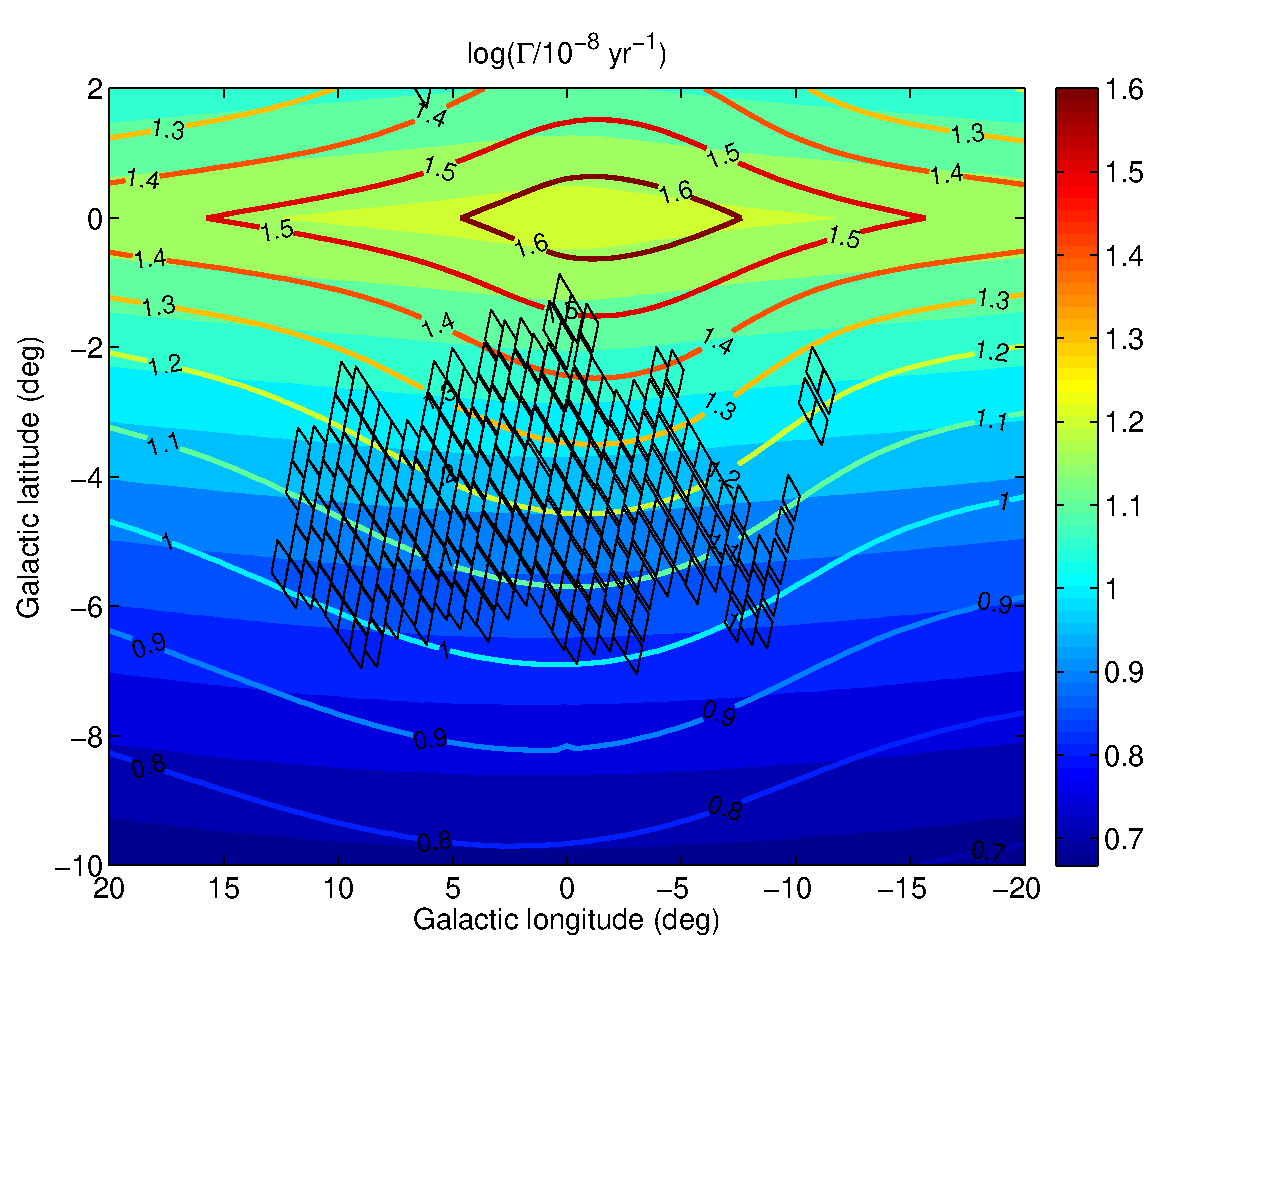
\includegraphics[width=4 in,trim=0 0 0 3cm]{map_event_ns.eps}
\caption{在银河系中心区域,由中子星导致的微引力透镜事件概率的等值图。
实线代表$\beta=-1$的结果,彩色区域代表$\beta=-2$的结果。OGLE-III的监测区域
用菱形表示。等值图采用对数取值的,$\log(\Gamma/10^{-8}$\,$\rm{yr^{-1}})$。}
\label{map_event}
\end{center}
\end{figure}
%%%%%%%%%%%%%%%%%%%%%%%%%%%%%%%%%%%%%%%%%%
%

在图\ref{map_event}中,我们给出了在银河系中心区域的由中子星导致的微引力
透镜事件的概率。等值图采用对数取值,$\log(\Gamma/10^{-8}$\,$\rm{yr^{-1}})$。
我们给出了两组结果,实线代表$\beta=-1$,彩色区域代表$\beta=-2$。
正如我们期待的,在银盘上的事件概率比较高,随着银纬的升高事件概率下降。
随着$\beta$从$-1$变到$-2$,事件概率的分布变得更扁更平,与高银纬的区域对比,
事件概率在银盘上随着银经的升高下降得更快。

微引力透镜事件的概率随着$\beta$的减小而下降,并且事件概率的分布变平是因为:
\begin{itemize}
\item $\beta$的减小意味着遥远的背景天体对事件概率的贡献减小了。因此事件概率
随着$\beta$的减小而下降。
\item 在银心方向,天体的密度比银盘上高。因此,$\beta$的减小对银心方向的影响
更大,银心方向的事件概率随着$\beta$的减小下降更快。
\item 在银河系核心区域,天体的速度弥散更大。因此$\beta$的减小使在银河系
中心方向,高速运动的背景天体的贡献减小。
\item 在银心后面的银盘上的天体绕银心运动的速度方向是与观测者和近距离的
透镜天体的速度方向相反的,于是透镜天体和背景天体的相对运动速度更快,对事件
概率的贡献也更大。$\beta$的减小意味着这部分遥远背景天体的贡献显著下降。
\end{itemize}

在图\ref{map_event}中,OGLE-III的监测区域\footnote{数据来自\url{http://ogle.astrouw.edu.pl/}}
使用菱形表示出。对于$340\times10^6$颗背景天体\supercite{Szymanski},并且
取$\beta=-1$,我们预计OGLE-III每年可以发现50个由中子星导致的微引力透镜事件,
同时我们有6\%的机会在九年的巡天期间发现一个由可观测射电脉冲星导致的事件。
目前正在进行中的OGLE-IV从2010年开始,覆盖了比OGLE-III大得多的天区,每年
发现四倍于OLGE-III的微引力透镜事件。因此,我们预计OGLE-IV每年将探测到约
200个由中子星导致的事件,并且在2020年之前有23\%的机会发现一个由可观测
射电脉冲星导致的微引力透镜事件。对于未来的更深、天区更广的光学巡天,我们
很有希望发现由可观测射电脉冲星导致的微引力透镜事件。比如,LSST预计将
监测$\sim10^{10}$颗银河系中的天体\supercite{ivez12a},取$\beta=-1$我们
估计每年将会发现约1000个由中子星导致的微引力透镜事件,以及约2个由可观测
射电脉冲星导致的事件。

值得指出的是,我们的计算很可能低估了photometric microlensing的事件概率。
我们在计算中使用Einstein半径作为引力透镜事件发生的截面,对应的背景天体亮度的
变化是约0.32\,mag。然而,在实际观测中我们有可能可以探测
到比这个更微弱的背景天体亮度的变化。假设我们可以观测到的背景天体的亮度
变化为0.1\,mag,那么事件概率将增大70\%。另外,实际的背景天体的数目有可能
因为不可区分的多个天体的叠加而被低估了\supercite{Smith07}。
  
\subsubsection{事件时标的分布}

通过将Monte Carlo integration的参数空间限制在某个特定的事件时标范围之内,
我们可以得到由中子星导致的微引力透镜事件的概率与时标的关系。我们的
结果展示在图\ref{timescale}中,我们取$\beta=-1$。全天平均事件概率
的时标的分布用实线表示。在银心和BW方向的事件概率的时标分布分别用点线和
虚线给出。我们指出,时标的分布在长时标和短时标上的渐进形式在WM05中已经
给出,我们的结果与渐进形式是符合的。我们发现,由中子星导致的微引力透镜
事件的时标分布都在约12天左右达到最大值。对于全天的平均事件概率以及在
银心和BW方向上的事件概率,平均时标分别是$\sim19.7$、$19.3$和$19.4$
天。作为对比,我们在图\ref{timescale}中也给出了WM05对中子星导致的事件
的时标的预测,其对应的平均时标是约47.3天。我们的结果说明,考虑了
中子星的空间和速度分布后,由中子星导致的事件的时标比之前工作的预计
短,这主要是因为中子星有比较高的速度。使用指数速度模型,我们得到
的全天平均事件概率的平均时标是约23.7天。

在图\ref{timescale_beta}中,我们展示了调整$\beta$对于银心方向的由中子星
导致的事件的时标分布的影响。当$\beta$从$-1$减小到$-2$,事件概率时标分布的变化
远比其他的$\beta$值大,这是因为当$\beta=-2$,根据式子\ref{rate}中的
$D_{\rm{s}}^{2+2\beta}$项,背景天体的密度开始随着距离的增加而减小。
对于时标比平均时标短的事件,改变$\beta$对事件概率的影响非常小。而对于
长时标的事件,改变$\beta$有明显的影响,随着$\beta$的减小事件概率降低。
然而,平均时标随着$\beta$的变化并不剧烈。取$\beta$在0到$-3$,平均时标
分别是19.3、17.9、13.5和13.2天。我们得到的平均时标的变化很难直观地
从物理图像上理解,因为随着$\beta$减小遥远的背景天体的贡献减小,我们预期
平均的透镜天体和背景天体的相对速度会减小,短时标的事件的概率会减小。
为了理解我们的结果,我们分别计算了平均的Einstein半径和透镜天体和背景天体
的相对速度。我们发现,随着$\beta$的减小,平均的Einstein半径和透镜天体
和背景天体的相对速度都减小,但是Einstein半径减小得更快。这就解释了随着
$\beta$减小平均时标减小。

%%%%%%%%%%%%%%%%%%%%%%%%%%%%%%%%%%%%%%%%%
\begin{figure}
\begin{center}
 % 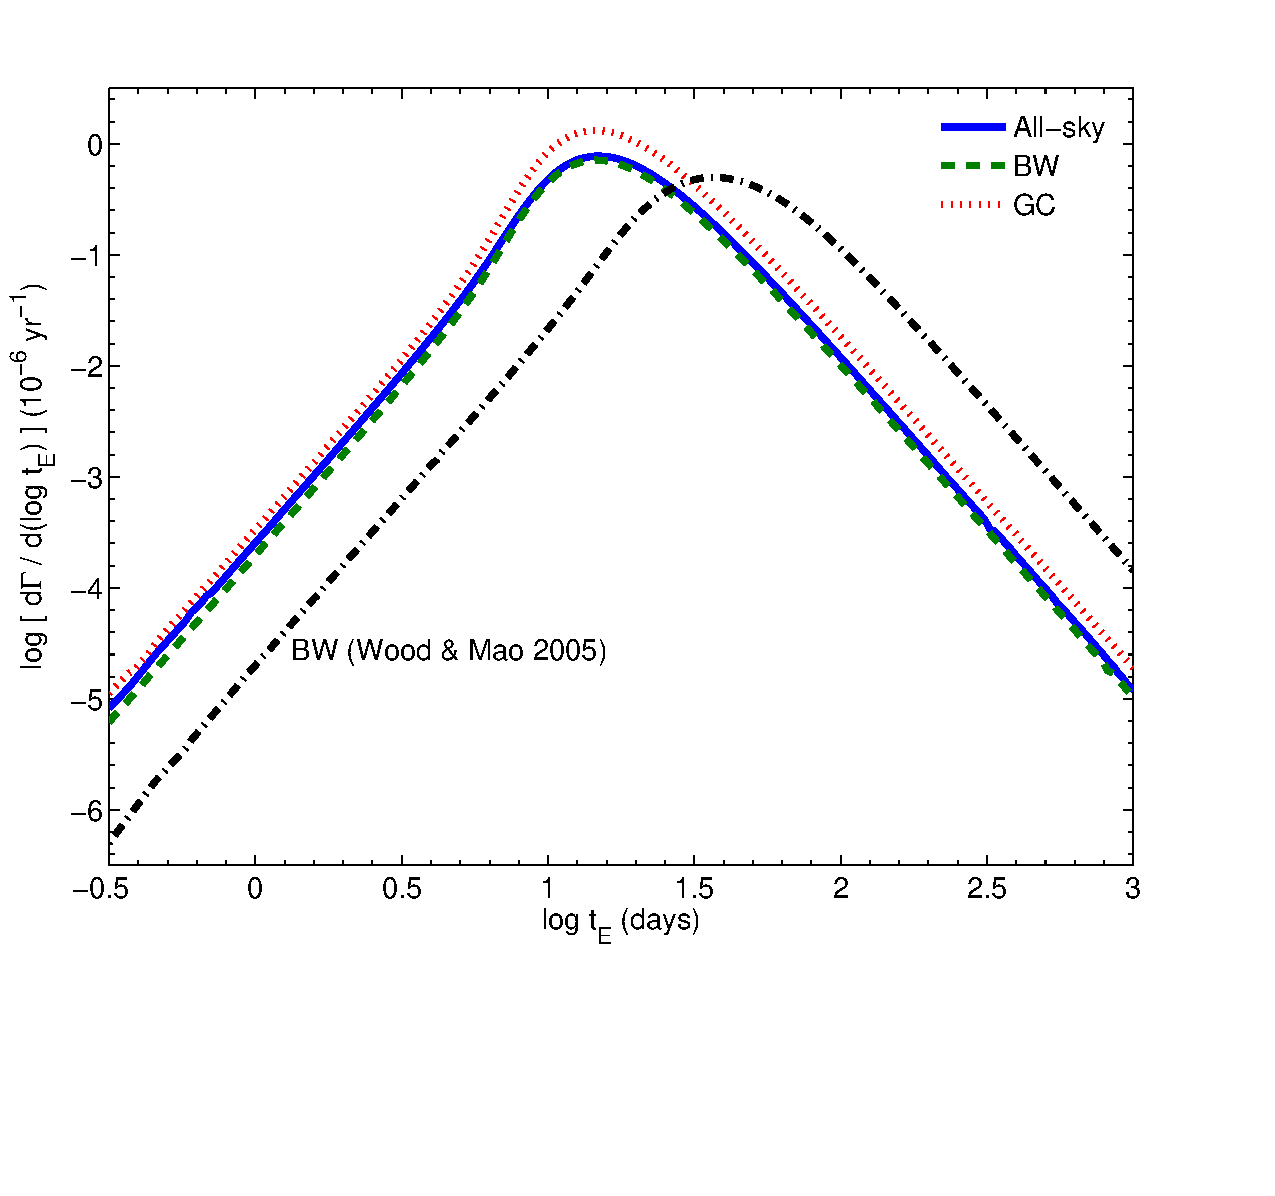
\includegraphics[width=4 in]{timescale.eps}
  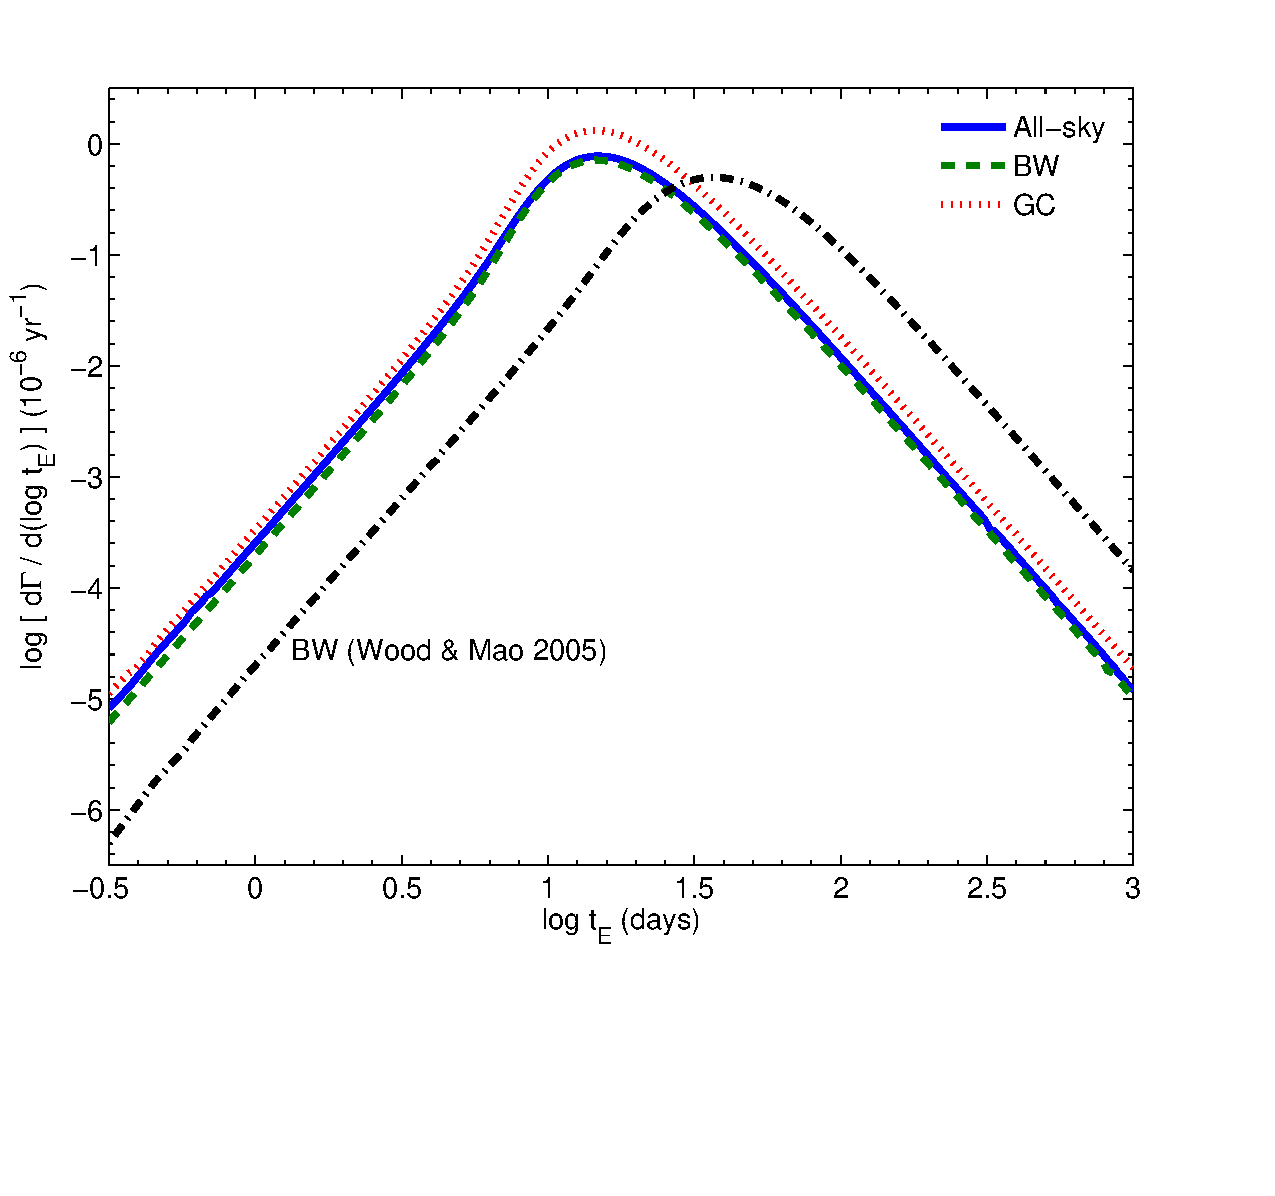
\includegraphics[width=4 in,trim=0 0 0 3cm]{timescale.eps}
\caption{中子星导致的微引力透镜事件的概率随时标的分布。实线、点线和虚线分别
对应全天事件概率、银心和BW方向的事件概率。作为对比,我们也给出了WM05的模型
对于中子星导致的事件的预言。}
\label{timescale}
\end{center}
\end{figure}
%%%%%%%%%%%%%%%%%%%%%%%%%%%%%%%%%%%%%%%%%

%
%%%%%%%%%%%%%%%%%%%%%%%%%%%%%%%%%%%%%%%%%
\begin{figure}
\begin{center}
  %
  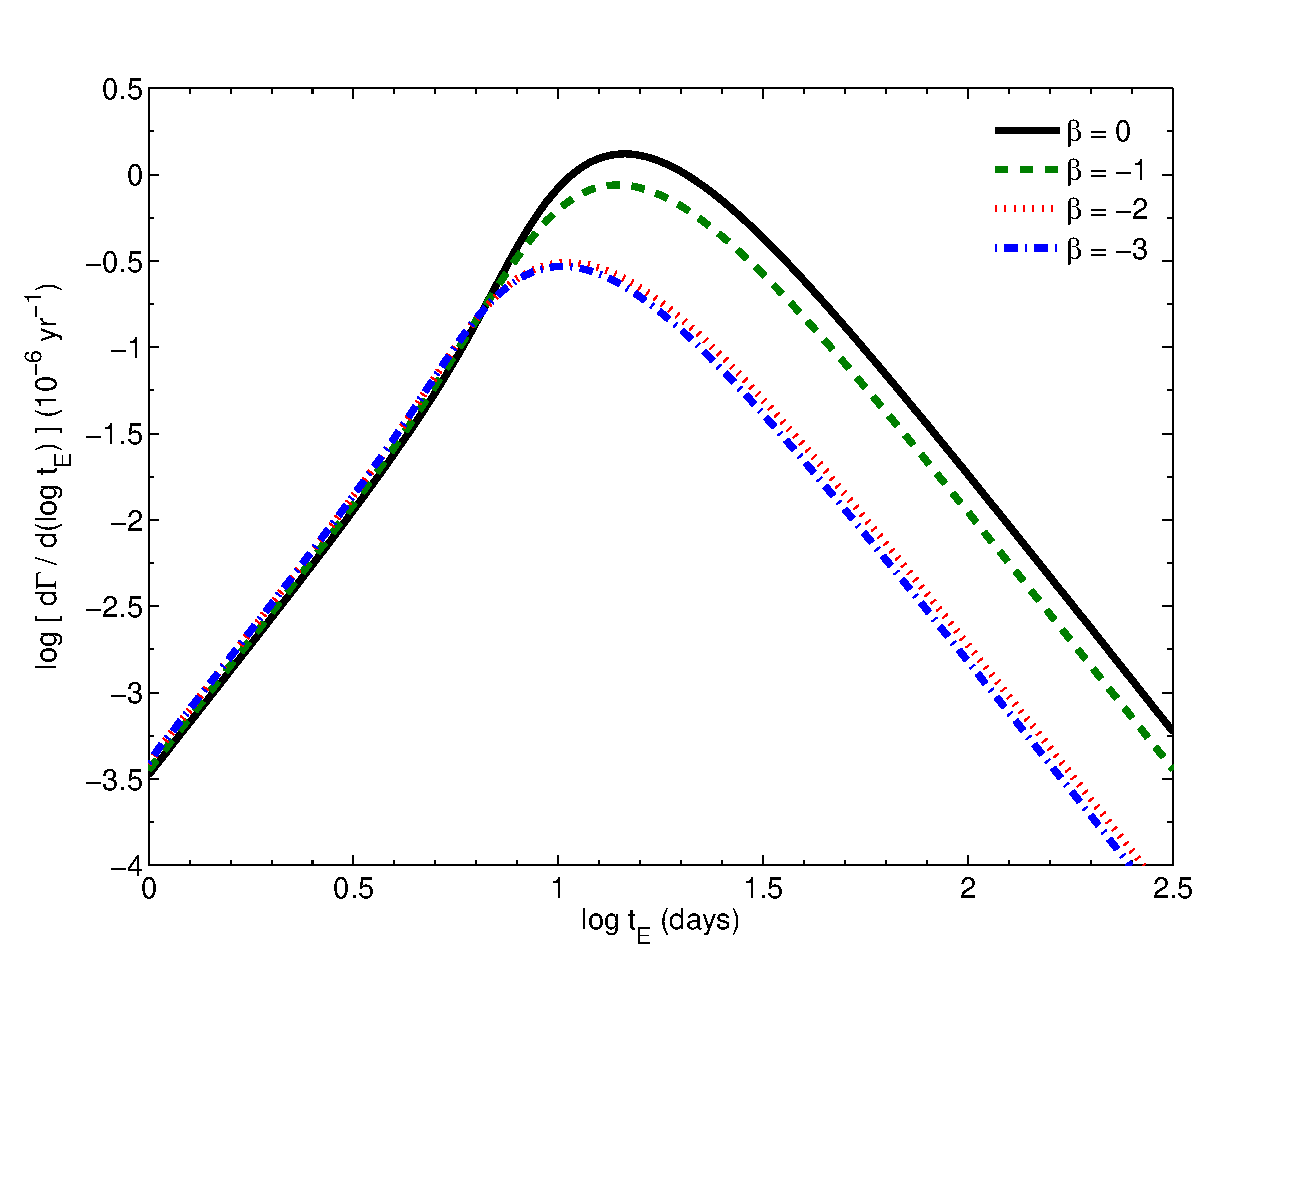
\includegraphics[width=4 in,trim=0 0 0 3cm]{time_beta.eps}
%
\caption{银心方向上中子星导致的微引力透镜事件的概率随时标的分布。实线、虚线、
点线和点虚线分别对应$\beta=0,-1,-2,-3$。}
\label{timescale_beta}
\end{center}
\end{figure}
%%%%%%%%%%%%%%%%%%%%%%%%%%%%%%%%%%%%%%%%%%
%

在WM05中,他们给出了在银心区域,平均的银河系微引力透镜事件(包含中子星
作为透镜天体以及其他天体作为透镜天体)的时标的等值图。我们计算得到的由中子
星导致的事件比较短的时标将降低平均的时标。在图\ref{map_timescale}中,
我们给出了银河系中心区域的微引力事件的平均时标的分布,可以与WM05中的
图3进行对比。实线代表$\beta=-1$的结果,彩色区域代表$\beta=-2$的结果。
OGLE-III的监测区域用菱形表示。在BW方向,取$\beta=0,-1,-2$,我们得到的
平均时标分别是23.3,23.9和36.5天。对于$\beta=0,-1$,我们的结果与WM05中
的结果接近,但是稍微小一些。我们的结果与OGLE观测的实际测量结果,$28.1\pm4.3$
天\supercite{sumi},是符合的。

%%%%%%%%%%%%%%%%%%%%%%%%%%%%%%%%%%%%%%%%%
%
\begin{figure}
\begin{center}
  %
  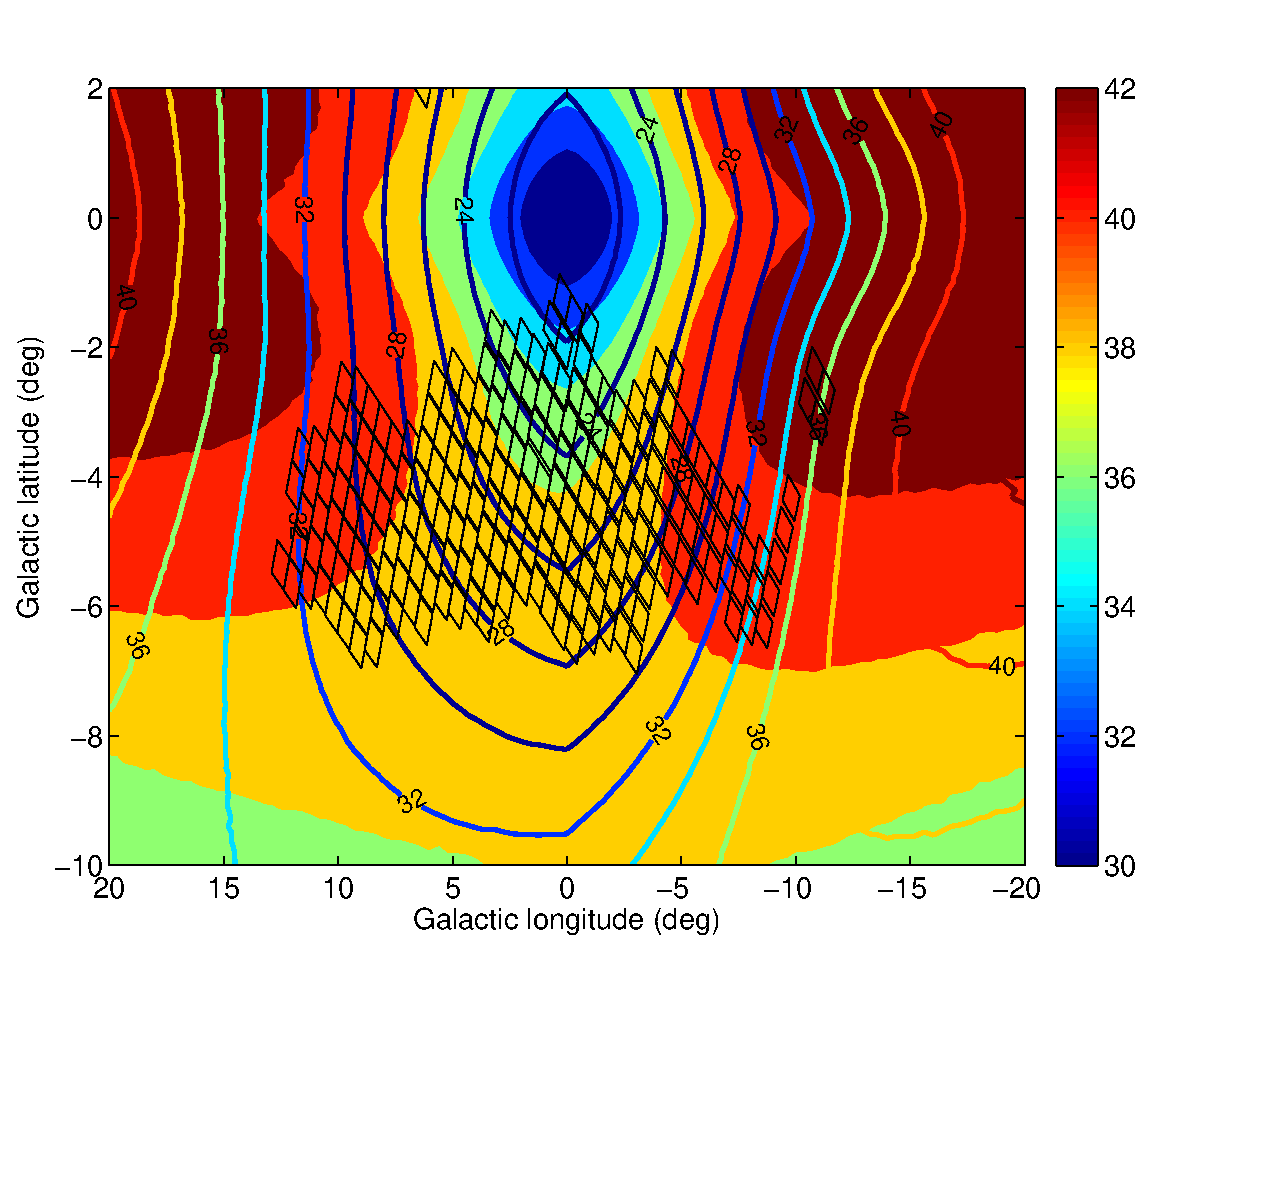
\includegraphics[width=4 in,trim=0 0 0 3cm]{map_timescale.eps}
%
\caption{银河系微引力透镜事件平均时标的等值图。实线对应$\beta=-1$,
彩色区域对应$\beta=-2$。等值线代表以天为单位的平均时标。OGLE-III区域
用菱形表示。}
\label{map_timescale}
\end{center}
\end{figure}
%%%%%%%%%%%%%%%%%%%%%%%%%%%%%%%%%%%%%%%%%%
%

\subsubsection{中子星导致的事件占银河系总事件的比例}

我们结果已经显示了由中子星导致的微引力透镜事件的时标比较短。Sumi et al. (2011)\supercite{sumi11}
预计由木星质量的天体导致的微引力透镜事件有更短的时标,而由其他的天体
导致的事件的时标则要更长。在这一节中,我们考虑在不同的时标上,
由中子星导致的事件占银河系总事件的比例。

在图\ref{ratio}中,我们给出了由中子星导致的事件所占的比例随着时标
的分布。实线代表BW方向的事件,虚线代表银心方向的事件。我们也
给出了远离银心方向($(l,b)=(-20^{\circ},0^{\circ})$ 
和$(l,b)=(0^{\circ},-10^{\circ})$)的结果。对于$(l,b)=(-20^{\circ},0^{\circ})$
(在银盘上,但是远离银心方向)中子星作为透镜天体的贡献在时标
短于约10天时可以高达约40\%,但是我们强调在这个方向上总的
事件概率远比银心方向低。在另外的三个方向上,中子星导致的事件
所占比例均在约15天的时标上达到最大值,并且也是分布的极大值。
我们的结果与之前的工作给出的预计不同,WM05的结果在图\ref{ratio}
中用点虚线表示。他们的工作显示中子星作为透镜天体的事件将主要
在几百天的时标上占较大比例,而在15天左右的时标上所占比例很低。
我们的工作则预计,中子星导致的事件将主要贡献银河系中的较短
时标的微引力透镜事件,这是因为中子星有比较高的速度。在远离
银心的方向上,随着短时标的银河系微引力透镜事件数目的下降,
中子星导致的事件所占短时标事件的比例快速上升。

%
%%%%%%%%%%%%%%%%%%%%%%%%%%%%%%%%%%%%%%%%%
\begin{figure}
\begin{center}
  %
  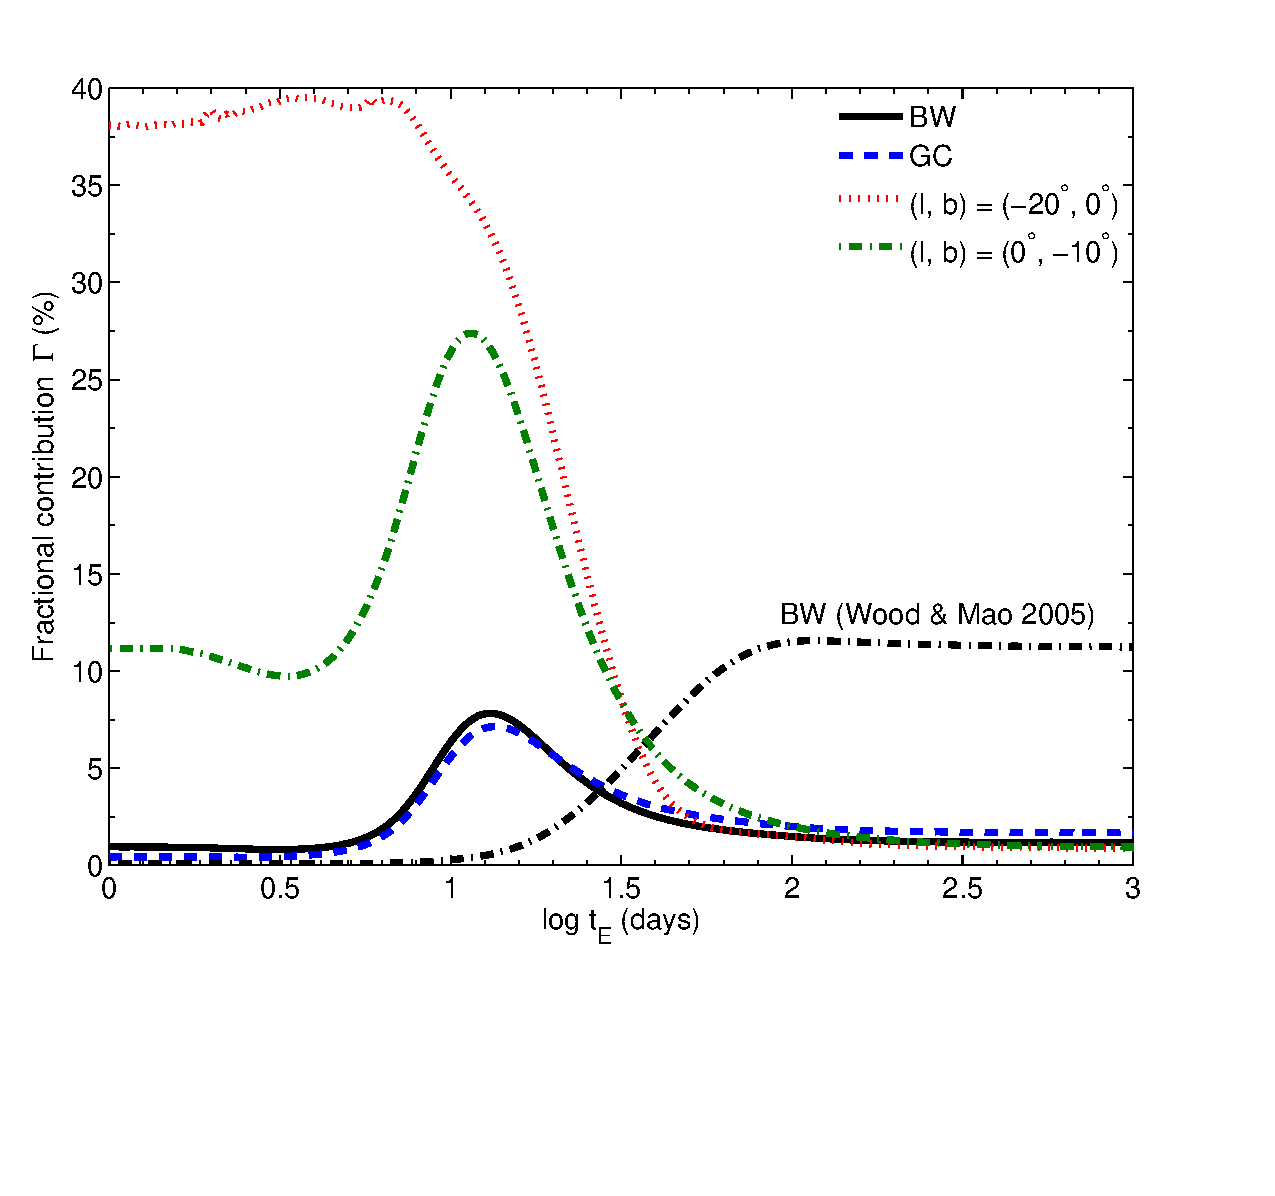
\includegraphics[width=4 in,trim=0 0 0 3cm]{ratio.eps}
%
\caption{中子星导致的微引力透镜事件占银河系总事件的比例随着事件时标的分布。
实线、虚线、点线和点虚线分别对应与BW、银心和远离银心方向($(l,b)=(-20^{\circ},0^{\circ})$
和$(l,b)=(0^{\circ},-10^{\circ})$)。作为对比,在BW方向上使用WM05的模型得到
结果也在图上画出。}
\label{ratio}
\end{center}
\end{figure}
%%%%%%%%%%%%%%%%%%%%%%%%%%%%%%%%%%%%%%%%%%
%

在图\ref{ratio_beta}中,我们给出了在银心方向上取不同的
$\beta$中子星作为透镜天体的贡献比。在所有情况下,贡献比都在约
10天的时标上达到最大值,并且都与WM05给出的结果不同。随着$\beta$
的减小,在10天左右的时标上由中子星导致的事件所占的比例升高。
对于$\beta=-3$,几乎所有的时标在10天左右的事件都是由中子星
导致的。
%
%%%%%%%%%%%%%%%%%%%%%%%%%%%%%%%%%%%%%%%%%
\begin{figure}
\begin{center}
  %
  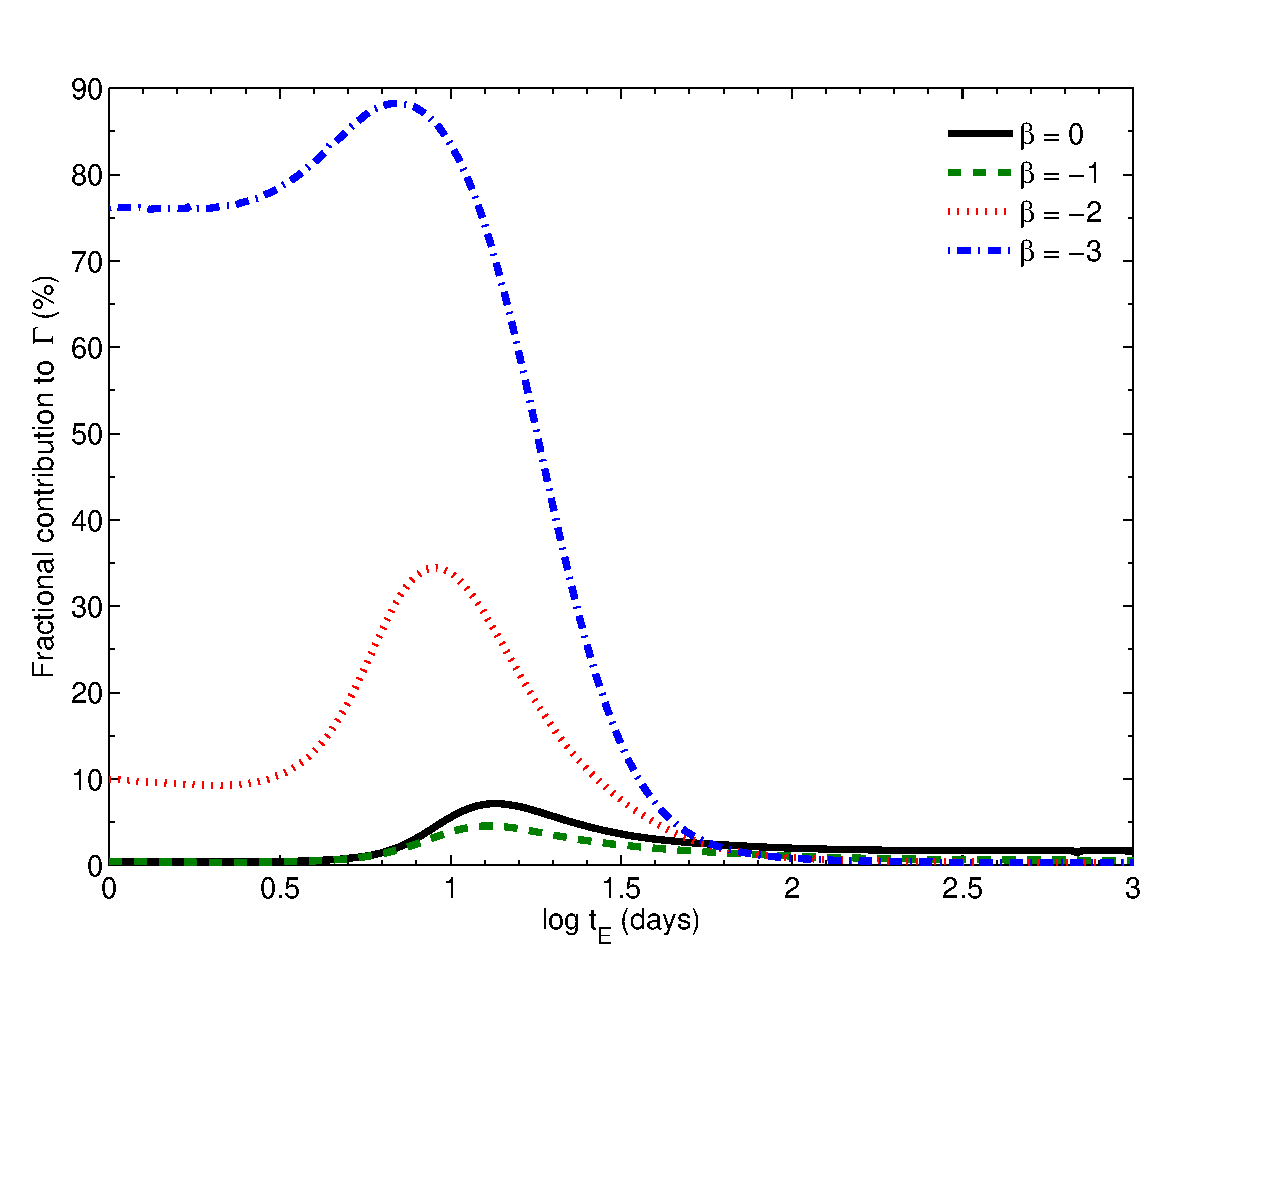
\includegraphics[width=4 in,trim=0 0 0 3cm]{ratio_beta.eps}
%
\caption{银心方向上,中子星导致的微引力透镜事件占银河系总事件的比例随着
事件时标的分布。实线、虚线、点线和点虚线分别对应$\beta=0,-1,-2,-3$。}
\label{ratio_beta}
\end{center}
\end{figure}
%%%%%%%%%%%%%%%%%%%%%%%%%%%%%%%%%%%%%%%%%%
%

中子星导致的事件占银河系总事件的比例在不同的方向上不同。在
图\ref{map_percentage}中,我们给出了中子星导致的事件所占比例
在银河系中心区域的等值图。实线对应$\beta=-1$,彩色区域对应
$\beta=-2$。OGLE-III的监测区域用菱形表示。中子星导致事件的比例
明显随着银经和银纬而变化,并且在远离银心区域所占比例比较高。
%
%%%%%%%%%%%%%%%%%%%%%%%%%%%%%%%%%%%%%%%%%
\begin{figure}
\begin{center}
  %
  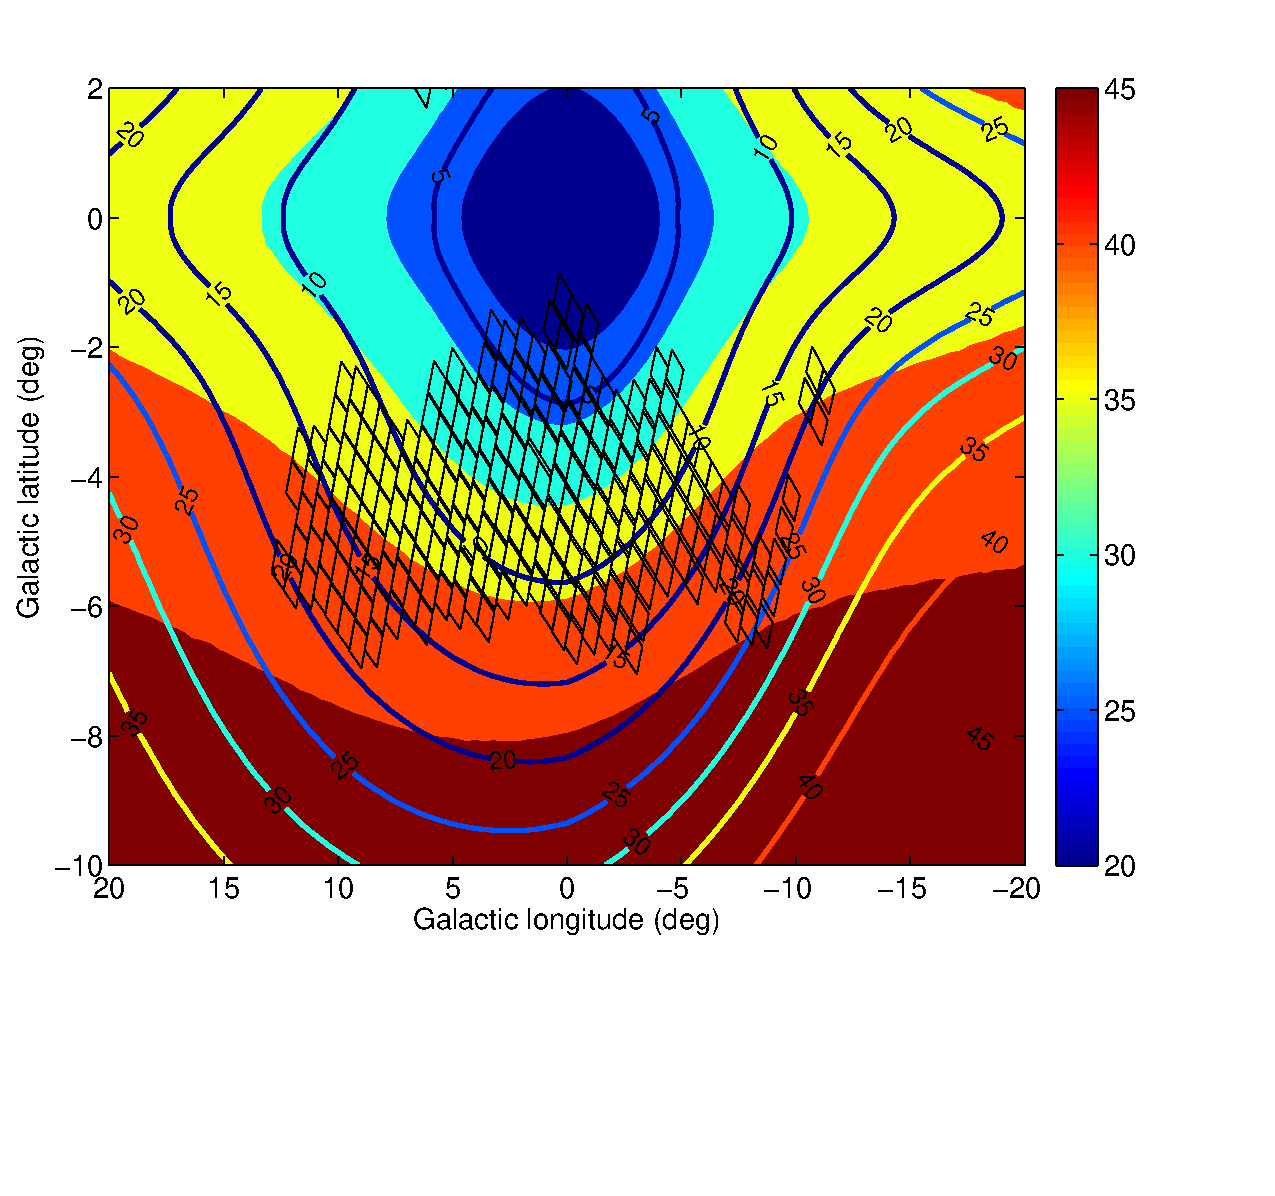
\includegraphics[width=4 in,trim=0 0 0 3cm]{map_percentage.eps}
%
\caption{中子星导致的微引力透镜事件占银河系总事件的比例的等值图。
实线对应$\beta=-1$,彩色区域对应$\beta=-2$。OGLE-III的监测区域用
菱形表示。}
\label{map_percentage}
\end{center}
\end{figure}
%%%%%%%%%%%%%%%%%%%%%%%%%%%%%%%%%%%%%%%%%%
%

在所有时标上进行平均,并且全天平均后,我们得到由中子星导致的微引力透镜
事件占银河系总事件的约5.4\%($\beta=0$)。在表\ref{percent}中,我们
给出了不同种类的天体作为透镜天体导致的事件占银河系总事件的比例。
我们的计算包含了褐矮星(BDs)、主序星(MSs)、白矮星(WDs)以及
黑洞(BHz)。我们也给出了对于不同的$\beta$值的结果。对于$\beta=0$,
中子星导致的事件所占比例比较低,然而随着$\beta$的下降,中子星导致事件
的贡献比例越来越高。通过增大和减小中子星速度分布的$\sigma$的30\%,
我们得到中子星导致的事件的贡献比分别为6.5\%和3.7\%($\beta=0$)。
使用指数的速度模型,我们得到的中子星导致事件的贡献比约是4.2\%($\beta=0$)。
%
%%%%%%%%%%%%%%%%%%%%%%%%%%%%%%%%%%%%%%%%%%%%%%%%%%%%%%%%%%%%%%%%%%%%%%%%%
\begin{table}
\begin{center}
\caption{不同种类的天体作为透镜天体对银河系总的事件概率的贡献比。
$\beta=-1,-2,-3$对应的结果被分别列出。作为对于,使用WM05模型得到
的结果也被列出。}
\label{percent}
%
\begin{tabular}{lccccc}
\hline
             &       \multicolumn{5}{c}{Types of lens}      \\
$\beta$      & BD   &    MS    &    WD     &  BH   & NS     \\
             &       \multicolumn{5}{c}{(per cent)}         \\
\hline
0            & 16.7 &    60.5  &    16.5   &  0.9  & 5.4    \\
-1           & 15.8 &    57.2  &    15.5   &  0.9  & 10.6   \\        
-2           & 10.6 &    38.2  &    10.4   &  0.5  & 40.3   \\         
-3           & 10.0 &    36.0  &    9.8    &  0.5  & 43.7   \\            
0 (WM05)     & 17.2 &    62.1  &    16.9   &  0.9  & 2.9    \\
\hline
\end{tabular}
\end{center}
\end{table}
%%%%%%%%%%%%%%%%%%%%%%%%%%%%%%%%%%%%%%%%%%%%%%%%%%%%%%%%%%%%%%%%%%%%%%%%%%
%
%

\subsection{通过astrometric microlensing测量脉冲星质量}

我们已经研究了由中子星导致的photometric microlensing事件的性质。
然而,由可观测射电脉冲星导致的photometric microlensing的事件概率
是比较低的,对于$10^{10}$颗背景天体,事件概率是约两个事件每十年。
由于astrometric microlensing事件发生的截面比photometric microlensing
事件大得多,更多的astrometric microlensing事件可能被探测到。目前
还没有可以预见的大规模的针对astrometric microlensing的巡天。于是
更可行的寻找由脉冲星导致的astrometric microlensing事件的方法是
使用已知的脉冲星的天体测量参数来预测引力透镜事件发生的时间和地点。
这个方法也可以用于搜寻由脉冲星导致的photometric microlensing事件,
但是astrometric microlensing更大发生截面意味着更高的成功概率。

我们用于计算photometric microlensing的事件概率的方法可以直接被
用于astrometric microlensing事件概率的计算,只需要使用更大的
发生截面。Astrometric microlensing的发生截面和现象的强度可以
使用“impact parameter ($u_0$)”来刻画。$u_0$是透镜天体和背景天体
之间角距离的最小值,单位是Einstein半径。于是astrometric microlensing
的事件概率可以直接根据截面增大的倍数放大photometric microlensing
的事件概率来估算。比如,如果astrometric microlensing的截面是
photometric microlensing的10倍(意味着$u_0=10$,在后面的小节中
会进一步讨论这个取值),那么假设$\beta=-1$以及$10^{10}$
颗背景天体,对于120000颗可观测的射电脉冲星,全天平均的事件概率是$\sim1.5$每年,

\subsubsection{Astrometric microlensing模型}

Belokurov \& Evans (2002)\supercite{Bel}(缩写为BE02)给出了
确定通过astrometric microlensing现象测量透镜天体质量的精度的
方法。他们说明了对于常规天体作为透镜天体的情况,有11个参数
需要通过观测确定。在我们后面的计算中,我们使用了BE02给出的方法,
但是我们主要是讨论射电脉冲星作为透镜天体的情况。

对于射电脉冲星作为透镜天体的情况,透镜天体的位置、自行以及
距离可以独立地通过射电观测得到。脉冲星的位置和自行可以通过
射电脉冲星的测时或者射电干涉观测确定。对于有多年观测数据
的射电脉冲星,通过测时得到的位置和自行的精度可以分别达到
$\leq 1$\,mas和$\leq 1$\,$\rm{mas\ yr^{-1}}$\supercite{verbiest}。
对于那些不能通过高精度测时来得到位置和自行的脉冲星,射电
干涉观测可以用于精确测量这些参数\footnote{我们指出,脉冲星测时
使用的dynamical solar system ephemeris与International Celestial 
Reference Frame (ICRF)不同。Madison et al. (2013)\supercite{Madison13}
计算了ICRF与脉冲星测时坐标系统的转换,并且讨论了在未来这样的
转化能如何通过更多的观测改进。}。在我们的模型中我们考虑一种
理想情况,假设射电脉冲星的位置和自行都是已知的参数,并且忽略
他们的测量误差。脉冲星的位置和自行的测量误差对我们的计算的影响
会在最后进行讨论。

脉冲星的距离相比位置和自行要更难确定。一些脉冲星的距离可以通过
视差的测量精确给出。但是对于大部分脉冲星来说,距离只能通过
色散测量(dispersion measures)来估算。通过色散测量来估计脉冲星
的距离依赖于银河系的自由电子密度分布的模型,而这一模型目前还不成熟,
于是导致通过这一方法估算距离的误差达到20\%\supercite{Taylor}。
尽管人们一直在改进银河系自由电子密度模型\supercite{cordes},但是
还不清楚到我们发现由脉冲星导致的微引力透镜事件时脉冲星的距离能不能
通过色散测量精确确定。因此,在我们的模型中我们考虑了两种情形。
第一种情形,称作Model $D_{\rm{psr}}^{\rm{known}}$,我们假设脉冲星
的距离是已知的;第二种情形,称作Model $D_{\rm{psr}}^{\rm{unknown}}$,
我们假设脉冲星的距离是未已知的。

对于Model $D_{\rm{psr}}^{\rm{known}}$,我们有六个独立参数需要
通过引力透镜效应的观测来确定,分别是背景天体的位置($\bm{\theta_{\rm{s,0}}}$)、
自行($\bm{\mu_{\rm{s}}}$)和视差($\pi_{\rm{s}}$),以及透镜天体的质量($M$)。
我们指出,背景天体的天体测量参数有可能也是精确知道的。这种情况下
我们只需要确定透镜天体的质量这一个参数,而在我们的工作中我们假设
这些参数是未知的,需要通过引力透镜效应的观测确定。对于Model $D_{\rm{psr}}^{\rm{unknown}}$,
我们还需要测量脉冲星的视差($\pi_{\rm{l}}$),于是有七个独立参数
需要确定。

我们考虑使用PSR B1929$+$10这颗脉冲星作为一个例子来研究。这颗脉冲星
有很大的自行(103\,$\rm{mas\ yr^{-1}}$)\supercite{Chatterjee04},
并且投影位置与多颗光学天体很近。根据我们对比已知脉冲星的位置\supercite{Manchester05}\footnote{http://www.atnf.csiro.au/research/pulsar/psrcat} 
与UKIRT Infrared Deep Sky Surveyd(UKIDSS)的源表\supercite{Lawrence}
的结果,在这颗脉冲星位置周围5\,arcsecs的范围内有七颗光学天体。
这颗脉冲星的距离是0.36\,kpc\supercite{Chatterjee04}。我们假设
这颗脉冲星很可能很近地经过一颗背景天体,并且我们进行一个持续四年
的对背景天体的位置的精确监测。我们假设观测采样在四年之内是均匀的,
并且以astrometric microlensing效应最强时作为时间中点。我们同时
假设背景天体的距离是5\,kpc,自行是7\,$\rm{mas\ yr^{-1}}$。

%
我们强调我们选择的透镜天体和背景天体的自行和距离不会影响我们
的研究的普遍性,因为astrometric microlensing效应的幅度是由并且
只由$u_0$决定。然而,透镜天体质量测量的精度与几个参数的选取有关。
首先是脉冲星的质量。在我们的计算中,我们使用$M=1.4$\,$\rm{M_{\odot}}$
作为典型的脉冲星质量,但是我们也尝试了其他的质量并且进行讨论。
其次我们需要假设背景天体的位置测量的精度。我们使用了两个可能
的取值,$\sigma=150$和450\,$\rm{\mu as}$。$\sigma=150$\,$\rm{\mu as}$
对应于\textit{Gaia}卫星对于一颗比较亮的源($V=16$\,mag)能达到的精度
\footnote{我们使用了\url{http://www.cosmos.esa.int/web/gaia/science-performance} 
提供的信息来估算单次观测的视差测量精度。对于$V=16$\,mag的
一个天体,\textit{Gaia}最终能达到的视差测量精度是约20-40\,$\rm{\mu as}$。
单次测量的视差精度会比这个差,约是这个值的4.3倍。单次观测的位置
测量的精度比视差测量的精度高,约是视差测量精度的0.743倍。于是我们
得到单次位置测量的精度大概是最终视差测量精度的三倍,约60-120\,$\rm{\mu as}$。
我们还需要考虑到\textit{Gaia}的单次观测只测量沿着扫描方向的一维的
位置,于是二维位置测量的精度需要乘以$\sqrt{2}$。考虑了以上因素之后
我们得到对于$V=16$\,mag的一个天体,单次二维位置测量的精度约是90-120\,$\rm{\mu as}$。
而对于更暗的天体($V=20$\,mag),\textit{Gaia}最终达到的视差测量
精度降到130-600\,$\rm{\mu as}$,这意味着单次二维位置测量的精度
只有0.5-3\,mas。}。未来的望远镜,比如Wide-Field Infrared Survey 
Telescope(WFIRST),即使对更暗的天体也能达到几十分之一毫角秒
的位置测量精度\supercite{Spergel}。最后我们还需要假设我们在整个
四年的监测中的观测频率,即总的观测数目。在我们的计算中我们尝试
了不同的观测频率,并进行了讨论。

\subsubsection{脉冲星质量测量}


图\ref{mass_u0}展示了脉冲星质量测量的误差随着$u_0$的变化。
脉冲星距离已知和未知的两种情形的结果都分别给出。我们使用
了两组不同的采样数,15和100次观测。我们的结果显示,质量测量
的误差在不同情形下变化很大。随着$u_0$的增大,质量测量的误差增大,
而随着采样数的增大,质量测量的误差减小。如果脉冲星的距离已知,
脉冲星的质量测量的误差只有距离未知情形的一半。我们指出,对于\textit{Gaia}卫星采样数大概是70\supercite{DeBruijne12}。
%
%%%%%%%%%%%%%%%%%%%%%%%%%%%%%%%%%%%%%%%%%
\begin{figure}
\begin{center}
  %
  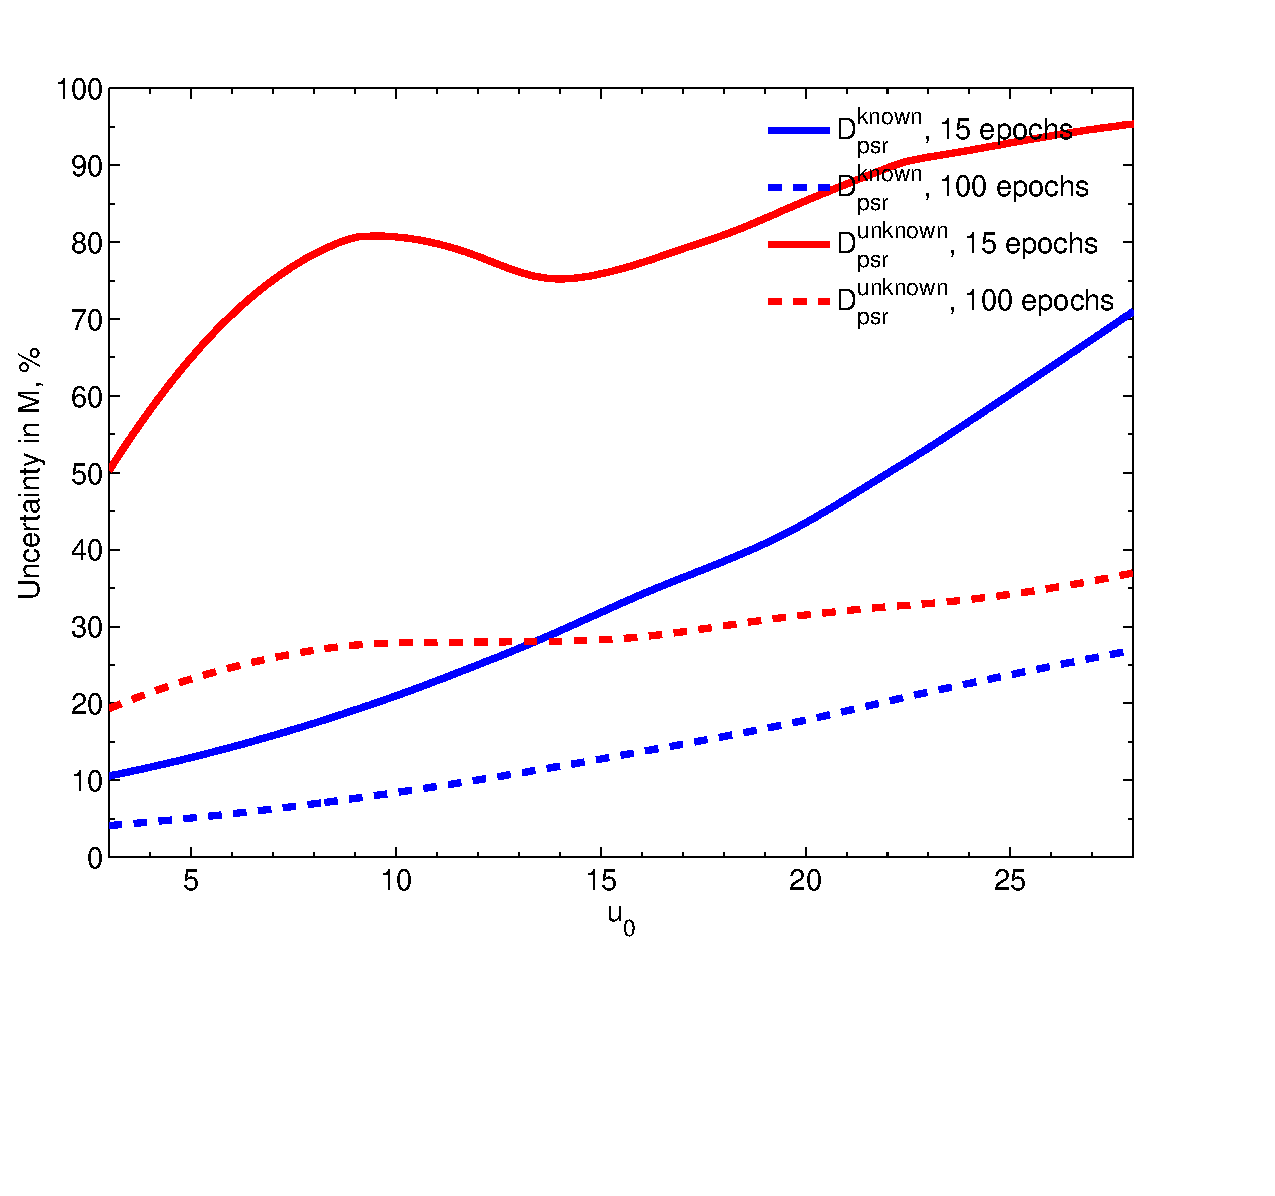
\includegraphics[width=4 in,trim=0 0 0 3.2cm]{u0_mass.eps}
%
\caption{质量测量的误差随着$u_0$的变化。误差是以
脉冲星质量为单位的。我们假设$M=1.4$\,$M_{\odot}$以及$\sigma=150$\,$\rm{\mu as}$。
实线和虚线分别代表采样数为$15$和$100$。红色和蓝色分别对应脉冲星距离
已知(Model $D_{\rm{psr}}^{\rm{known}}$)和未知(Model $D_{\rm{psr}}^{\rm{unknown}}$)的情形。
}
\label{mass_u0}
\end{center}
\end{figure}
%%%%%%%%%%%%%%%%%%%%%%%%%%%%%%%%%%%%%%%%%%

图\ref{mass_6}和\ref{mass_7}给出了质量测量的误差随观测的数目的变化。
在图\ref{mass_6}中,我们假设脉冲星距离是已知的,而在图\ref{mass_7}
中我们假设脉冲星距离是未知的。在两张图中,我们都给出了$u_0=10$和$u_0=30$,
以及$\sigma=150$\,$\rm{\mu as}$和$\sigma=450$\,$\rm{\mu as}$的四组结果。
我们发现,当观测数目大于$\sim$100时,质量测量的误差便几乎不再变化,
这说明更高的监测频率不是必须的,不会提高质量测量的精度。当背景天体
的位置测量精度从450\,$\rm{\mu as}$提高到150\,$\rm{\mu as}$,透镜
天体的质量测量精度提高了两倍。因此,为了精确地确定脉冲星的质量,
我们需要高精度的背景天体的位置测量。

%
%%%%%%%%%%%%%%%%%%%%%%%%%%%%%%%%%%%%%%%%%
\begin{figure}
\begin{center}
  %
  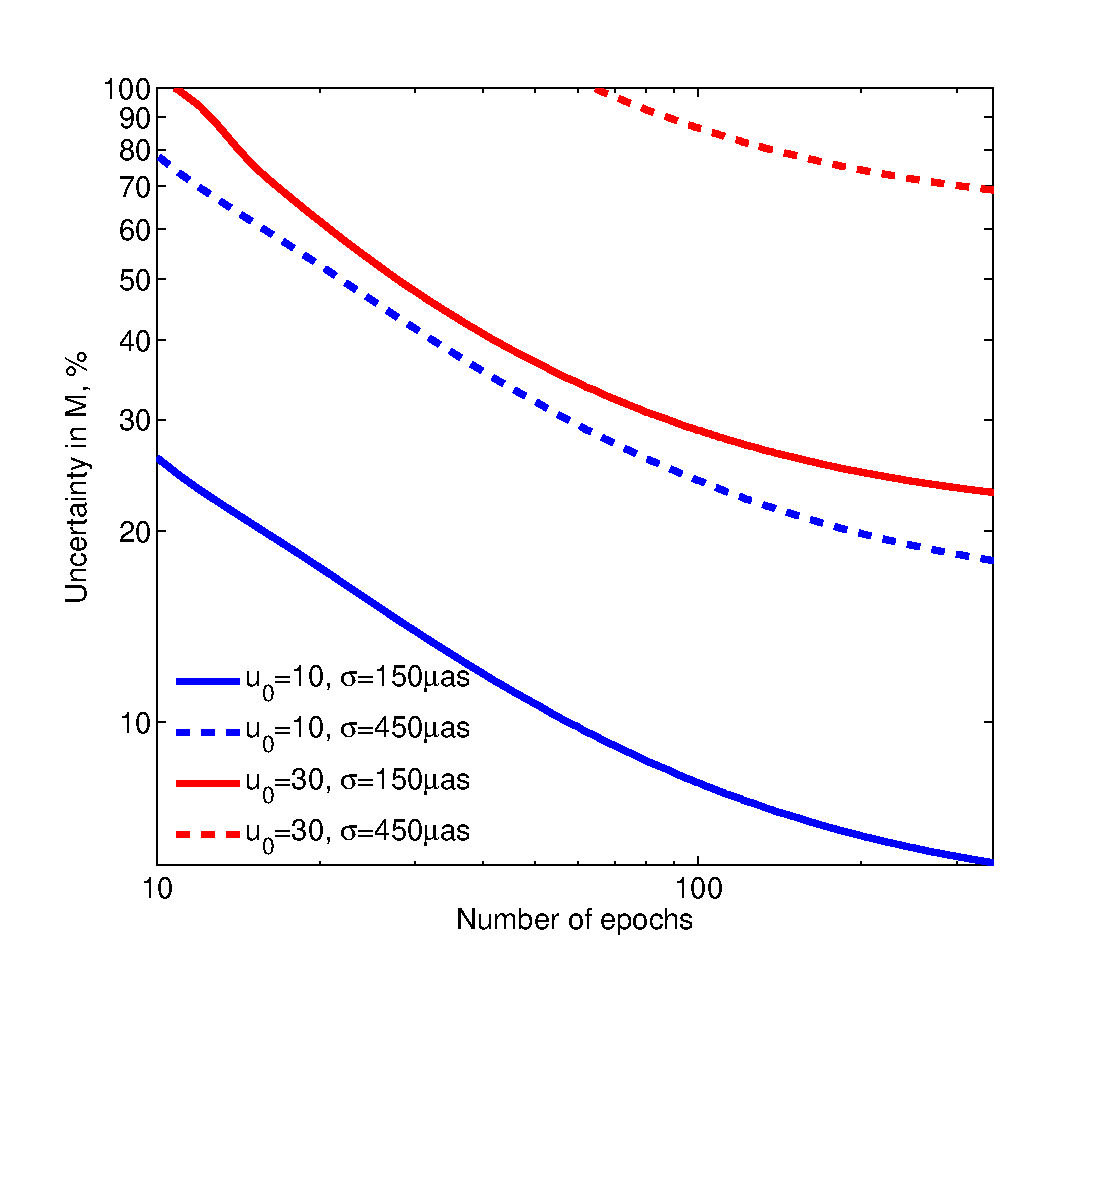
\includegraphics[width=4 in,trim=0 0 0 3.2cm]{mass_6.eps}
%
\caption{质量测量的误差随着观测数目的变化。误差是以
脉冲星质量为单位的。我们假设$M=1.4$\,$M_{\odot}$,并且假设
脉冲星的距离已知(Model $D_{\rm{psr}}^{\rm{known}}$)。
我们给出了对应不同的$u_0$和$\sigma$的结果。
}
\label{mass_6}
\end{center}
\end{figure}
%%%%%%%%%%%%%%%%%%%%%%%%%%%%%%%%%%%%%%%%%%
%
%
%%%%%%%%%%%%%%%%%%%%%%%%%%%%%%%%%%%%%%%%%
\begin{figure}
\begin{center}
  %
  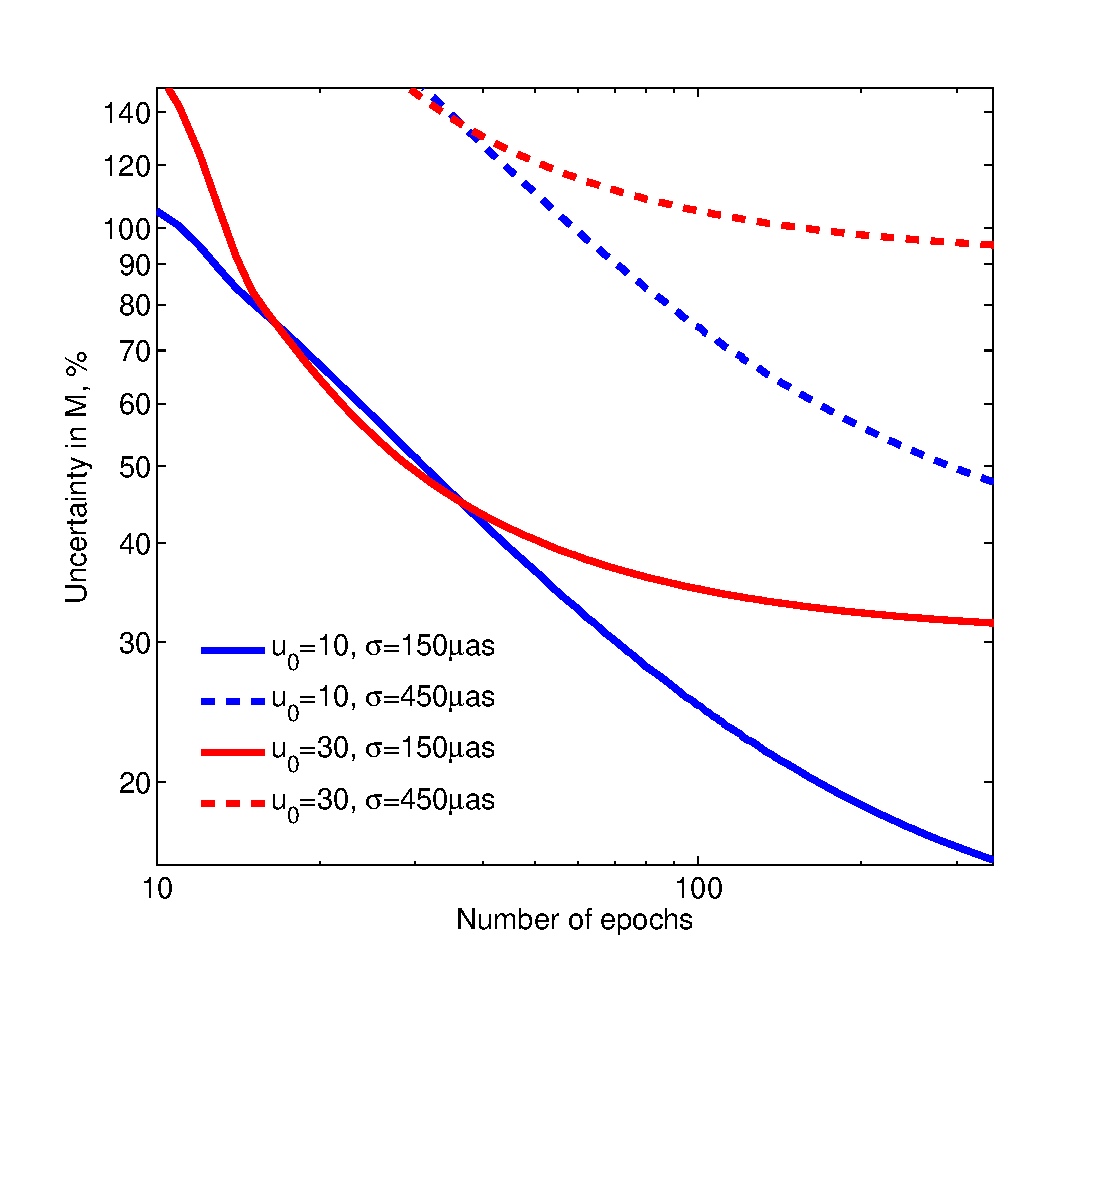
\includegraphics[width=4 in,trim=0 0 0 3.2cm]{mass_7.eps}
%
\caption{质量测量的误差随着观测数目的变化。误差是以
脉冲星质量为单位的。我们假设$M=1.4$\,$M_{\odot}$,并且假设
脉冲星的距离未知(Model $D_{\rm{psr}}^{\rm{unknown}}$)。
我们给出了对应不同的$u_0$和$\sigma$的结果。
}
\label{mass_7}
\end{center}
\end{figure}
%%%%%%%%%%%%%%%%%%%%%%%%%%%%%%%%%%%%%%%%%%
%

在图\ref{masses}中,我们假设了不同的脉冲星质量,并且假设脉冲星
距离已知(Model $D_{\rm{psr}}^{\rm{known}}$),然后给出了质量
测量的误差随着观测数目的变化。我们假设$u_0=10$以及$\sigma=450$\,$\rm{\mu as}$。
除了典型的脉冲星质量,1.4\,$\rm{M_{\odot}}$,我们还使用了极低的
脉冲星质量,0.4\,$\rm{M_{\odot}}$,和极大的脉冲星质量,2.4\,$\rm{M_{\odot}}$。
我们发现,随着脉冲星质量的增大,质量测量的误差减小。对于大质量
脉冲星的情形(2.4\,$\rm{M_{\odot}}$),质量测量的误差比小质量脉
冲星的情形(0.4\,$\rm{M_{\odot}}$)小六倍。
%
%%%%%%%%%%%%%%%%%%%%%%%%%%%%%%%%%%%%%%%%%
\begin{figure}
\begin{center}
  %
  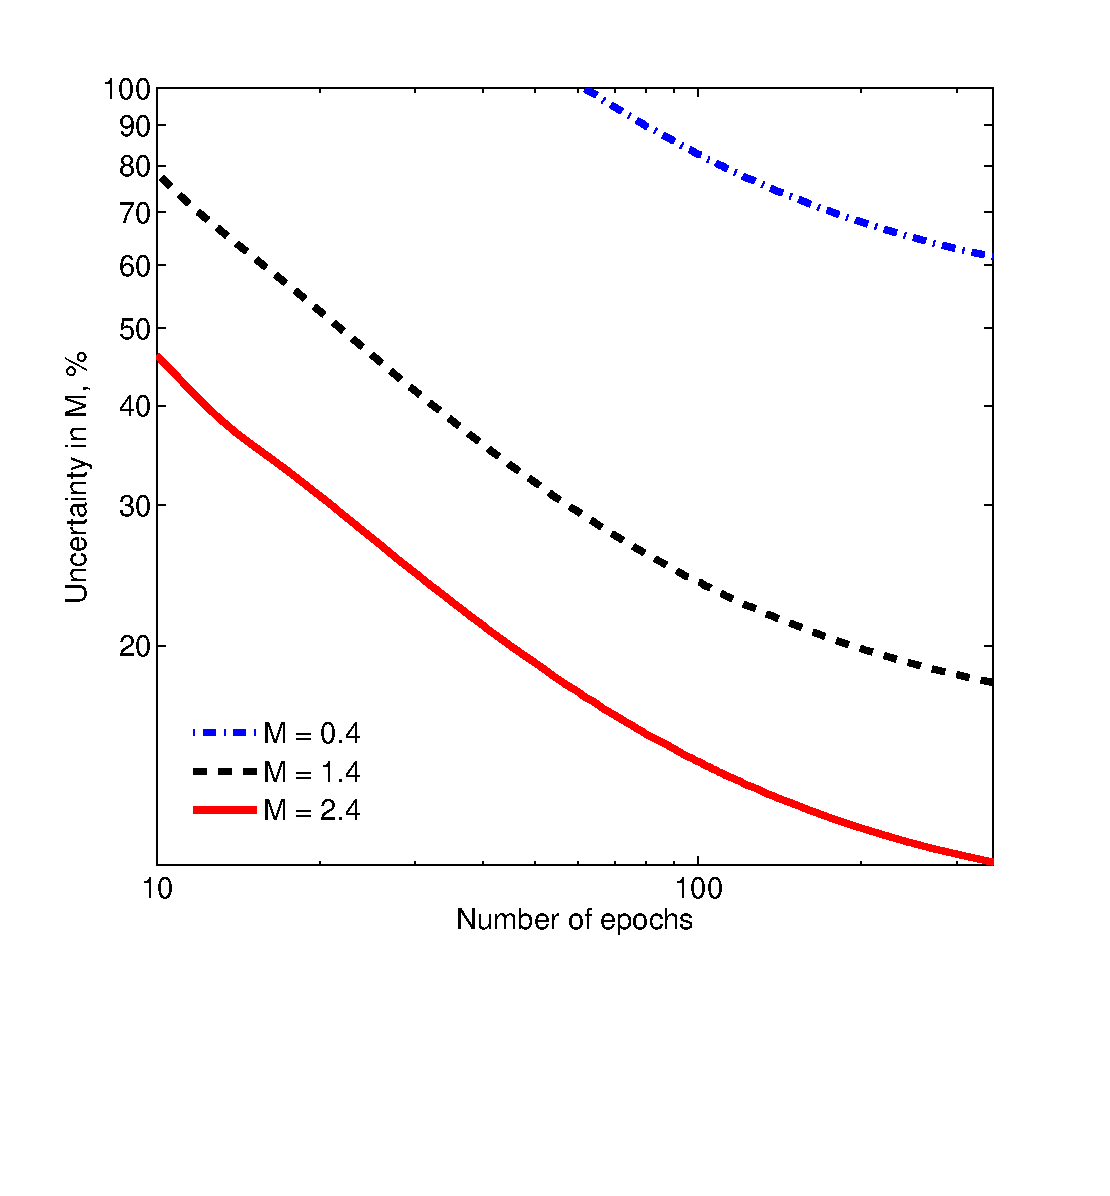
\includegraphics[width=3.5 in,trim=0 0 0 3.2cm]{masses.eps}
%
\caption{质量测量的误差随着观测数目的变化。误差是以脉冲星质量为
单位的。我们分别取$M=0.4,1.4,2.4$\,$M_{\odot}$。
我们假设脉冲星距离已知(Model $D_{\rm{psr}}^{\rm{known}}$)。
}
\label{masses}
\end{center}
\end{figure}
%%%%%%%%%%%%%%%%%%%%%%%%%%%%%%%%%%%%%%%%%%
%

在以上的计算中,我们假设了一种理想情况,即脉冲星的位置和自行可以被精确地
测量并且测量误差可以被忽略不计。如果脉冲星的天体测量参数不能被独立地测量,
那么我们将需要通过引力透镜效应的观测来确定它们,从而将降低我们测量
透镜天体质量的精度。现在我们讨论一种中间情形,脉冲星的位置和自行可以
被独立地测量,但是测量误差不能被忽略。我们将这些参数的误差模拟为背景天体
位置测量的误差,然后使用相同的方法来研究透镜天体质量测量的精度。我们
假设脉冲星位置和自行测量的误差分别为0.01\,$\rm{mas}$和0.1\,$\rm{mas\ yr^{-1}}$。
这是目前通过Very Long Baseline Interferometry(VLBI)可以达到的精度\supercite{deller}。
假设脉冲星距离已知(Model $D_{\rm{psr}}^{\rm{known}}$)以及$u_0=10$和
50次观测,我们发现脉冲星质量的误差从约10\%增加到12\%。对于更大的脉冲星
位置和自行的误差,0.1\,$\rm{mas}$和1\,$\rm{mas\ yr^{-1}}$,质量测量的
误差约为22\%。因此我们得出结论,脉冲星的位置和自行的误差将引入额外
的质量测量误差,但是影响比较小,而且通过提高脉冲星位置和自行
的精度可以降低这一影响。

\subsection{小结}

有多个测光的大型巡天正在或者即将在不远的将来开始,这些巡天项目将主要
集中在银河系中心和银盘上,比如OGLE-IV、Vista Variable in the Via Lactea~\supercite{Minniti} 
和WFIRST~\supercite{Spergel}。在不远的将来LSST\supercite{ivez}将每三天
监测10000平方度的天区两次。
这样的巡天预计将对$r\sim24.5$ (AB)的点源达到$5\sigma$的深度的观测。
目前还不清楚LSST是否会搜寻银盘和银核,即使不会大范围地监测银盘和银核,
LSST也将监测$10^{10}$量级的银河系天体;而如果包含银盘和银核,监测
的银河系天体的数目将更大。另外,一个三年的HST项目计划发现在银河系中心
方向的由银河系内的黑洞和中子星导致的微引力透镜事件\supercite{sahu}。

我们的计算表明:
\begin{itemize}
\item 由中子星导致的微引力透镜事件的时标比之间预计的短,只有约20天左右。
\item 在银河系中心方向,在时标为15天左右的事件中,有大约7\%是由中子星
导致的。而在远离银心方向,对于时标短于20天的事件,由中子星导致的事件
所占的比例将高达40\%。
\item 通过astrometric microlensing效应,如果脉冲星的距离已知,脉冲星的
质量测量的精度可以达到约10\%。通过足够多的观测次数,即使脉冲星的距离
未知,脉冲星的质量也可以测量精确到25\%/。
\end{itemize}

对于正在进行中的巡天,我们建议:
\begin{itemize}
\item 为了能尽可能多的探测到由中子星导致的微引力透镜事件,巡天应该
集中在银盘和银河系中心区域。
\item 为了发现由中子星导致的微引力透镜事件,我们应该集中搜寻短时标的
微引力透镜事件,并使用射电望远镜定点观测这些候选体以发现射电脉冲星。
\item 当新的射电脉冲星被发现后,他们的天体测量参数应该被精确的测量,
并且与已知的光学巡天结果进行对比。如果发现脉冲星有可能经过背景天体,
引发astrometric microlensing效应,那么我们可以预测事件发生的时间并
使用光学望远镜监测这个背景天体。
\item 尽管通过射电脉冲星的参数预测微引力透镜事件并使用光学望远镜
定点观测是最佳的策略,但是像\textit{Gaia}卫星这样的项目也不可忽视。
\textit{Gaia}总共将观测$10^9$颗银河系天体,根据我们的估算,在整个
项目期间(五年)将发现一个由脉冲星导致的事件。
\end{itemize}

在更远的将来,大的射电望远镜将发现大部分银河系内可观测的射电脉冲星。
因此我们很可能发现由可观测的射电脉冲星导致的微引力透镜事件,并以此
测量脉冲星的质量。这样的测量将促进我们对中子星的理解,并且揭示
中子星的内部结构和致密物质的物态。

\pkuthssffaq


	% vim:ts=4:sw=4
% Copyright (c) 2014 Casper Ti. Vector
% Public domain.

\def\qui {1E 1547-54}
\def\uu {4U~0142$+$61}
\def\oo {1E~1048$-$59}
\def\kes {1E~1841$-$045}
\def\axj {AX~J1845$-$02}
\def\rxs {1RXS~J1708$-$40}
\def\eee {1E~2259$+$586}
\def\xte {XTE~J1810$-$197}
\def\cxo {CXOU~J1647$-$45}
\def\smc {CXOU~J0100-72}
\def\zerosei {SGR~1806$-$20}
\def\zerozero {SGR~1900$+$14}
\def\sedici {SGR~1627$-$41}
\def\lmc {SGR~0526$-$66}
\def\quil {1E 1547.0-5408}
\def\uul {4U~0142$+$61}
\def\ool {1E~1048$-$586}
\def\kesl {1E~1841$-$045}
\def\axjl {AX~J1844.8$-$0256}
\def\rxsl {1RXS~J170849$-$400910}
\def\eel {1E~2259$+$586}
\def\xtel {XTE~J1810$-$197}
\def\cxol {CXOU~J164710.2$-$455216}
\def\smcl {CXOU~J010043.1-721134}

\chapter{X射线波段的研究}

\section{反常X射线脉冲星和软伽马射线重复爆的硬X射线辐射}

反常X射线脉冲星(Anomalous X-ray pulsars,AXPs)和软伽马射线重复爆(soft gamma-ray 
repeaters,SGRs)是两类特殊的脉冲星类致密天体。反常X射线脉冲星是首先作为软X射线源
发现的($<$10\,keV)\supercite{fg81,scs86,ims94},而软伽马射线重复爆则是作为
硬X射线波段的短爆发现象被发现的\supercite{mgg+79,mgi+79}。我们已经发现软伽马射线
重复爆的持续X射线辐射对应体,也发现了反常X射线脉冲星有爆发现象,因此现在普遍认为
反常X射线脉冲星和软伽马射线重复爆是同一类脉冲星类致密天体\supercite{m08}。
%
经过十多年的多波段的观测和研究,我们发现了反常X射线脉冲星和软伽马射线重复爆的多种
多样的现象。在这一类天体背后的极端的天体物理环境吸引众多天体物理学家的目光\supercite{m08}。

反常X射线脉冲星和软伽马射线重复爆最主要的两个特征是没有伴星的证据和X射线光度
大于自转能损。这两个特征将反常X射线脉冲星和软伽马射线重复爆与其他X射线脉冲星
区分开来。反常X射线脉冲星和软伽马射线重复爆有很多相同点,比如相似的自转周期
自转周期的导数,比较窄的自转周期的分布,没有射电辐射以及与超新星遗迹成携。
表\ref{tab-list1}和\ref{tab-list2}列出了现在已知的反常X射线脉冲星和软伽马射线
重复爆\supercite{m08}。

%%%%%%%%%%%%%%%%%%%%%%%%%%%%%%%%%%%%%%%%%%%%%%%%%%%%%%%%%%%%%%%%%%%%%%%%%%%%%%%%%%%%
\begin{table}
\caption{目前已知的反常X射线脉冲星~\supercite{m08}。}
 \centering
\label{tab-list1}
\begin{tabular}{lcccc}
\hline\noalign{\smallskip}
Name           &Hard X-rays$^{(a)}$& Soft X-rays$^{(a)}$          & Distance      & Location \\[3pt]
               &  ($>$10 keV)      & ($<$10 keV)                  & (kpc)         &  \\[3pt]
\hline
\multicolumn{5}{c}{\textbf{Anomalous X--ray Pulsars}}\\ [3pt]
 \hline
\smc           & -                 & P                            &  61           & SMC \\[3pt]
\cite{lfmp02}  &                   & \cite{lfmp02}                &               &     \\[3pt]
 \hline
\uu            & P                 & P                            &  3.6          &     \\[3pt]
\cite{ms95}    & \cite{dhk+06}     & \cite{ims94}                 &\cite{dv06a}   &     \\[3pt]
\hline
\oo            & D                 & P                            & 9             &     \\[3pt]
\cite{ms95}    & \cite{lwr08}      & \cite{scs86}                 &\cite{dv06a}   &     \\[3pt]
\hline
\qui           & -                 & P,T                          & 9             & SNR G327.24--0.13 \\[3pt]
\cite{gg07}    &                   & \cite{hgr+08}                &\cite{ccr+07}  &     \\[3pt]
\hline
\cxo           &     -             & P,T                          & 3.9           & Massive Star Cluster \\[3pt]
\cite{mcc+06}  &                   &\cite{mcc+07}                 &\cite{kd07}    &  Westerlund 1     \\[3pt]
\hline
\rxs           & P                 & P                            & 3.8           &      \\[3pt]
\cite{snt+97}  & \cite{khd+06}     &\cite{snt+97}                 &\cite{dv06a}   &      \\[3pt]
\hline
\xte           & -                 & P,T                          & 3.1           &      \\[3pt]
\cite{ims+04}  &                   &\cite{ims+04}                 &\cite{dv06a}   &      \\[3pt]
\hline
\kes           & P                 & P                            & 8.5           & SNR Kes 73\\[3pt]
\cite{vg97}    & \cite{khm04}      & \cite{vg97}                  & \cite{tl08}   &     \\[3pt]
\hline
\axj $^{(b)}$  & -                 & P,T                          & 8.5           & SNR G29.6+0.1 \\[3pt]
\cite{tkk+98}  &                   & \cite{tkk+98}                & \cite{tkk+98} &     \\[3pt]
\hline
\eee           & -                 & P                            & 7.5           & SNR CTB 109 \\[3pt]
\cite{ms95}    &                   &\cite{fg81}                   & \cite{dv06a}  &     \\[3pt]
\hline
 \hline
\end{tabular}
\end{table}

%%%%%%%%%%%%%%%%%%%%%%%%%%%%%%%%%%%%%%%%%%%%%%%%%%%%%%%%%%%%%%%%%%%%%%%%%%%%%%%%%%%%
\begin{table}
\caption{目前已知的软伽马射线重复爆~\supercite{m08}。}
 \centering
\label{tab-list2}
\begin{tabular}{lcccc}
\hline\noalign{\smallskip}
Name           &Hard X-rays$^{(a)}$& Soft X-rays$^{(a)}$          & Distance      & Location \\[3pt]
               &  ($>$10 keV)      & ($<$10 keV)                  & (kpc)         &  \\[3pt]
\hline
\multicolumn{5}{c}{\textbf{Soft Gamma-ray Repeaters}} \\ [3pt]
 \hline
\lmc           & -                 & P                            & 55            & LMC, SNR N49 \\[3pt]
\cite{cdp+80}  &                   & \cite{rkl94}                 &               &     \\[3pt]
\hline
\sedici        & -                 & D,T                          & 11            & \\[3pt]
\cite{wkv+99}  &                   & \cite{wkv+99}                & \cite{ccdd99} &     \\[3pt]
\hline
\zerosei       & D                 & P                            & 15            & Massive Star Cluster \\[3pt]
\cite{lff+86}  &\cite{mgm+05}      &\cite{kds+98}                 & \cite{ce04}   &     \\[3pt]
\hline
\zerozero      & D                 & P                            & 15            & Massive Star Cluster \\[3pt]
\cite{mgg+79}  & \cite{gmt+06}     &\cite{hkw+99}                 & \cite{vhl+00} &     \\[3pt]
\hline
 \hline
\end{tabular}

\textbf{Notes:}

$^{(a)}$ D = detection; P = pulsations detected; T = transient

$^{(b)}$ Candidate AXP (no $\dot P$ measurement)
\end{table}

\subsection{谱的性质}

尽管反常X射线脉冲星和软伽马射线重复爆的距离很难精确地确定,但是粗略的估计可以
通过X射线的吸收和成携的超新星遗迹的距离得到。典型的距离在至少几个kpc的量级,
意味着典型的光度在$10^{34-36}$\,$\rm{erg\ s^{-1}}$的量级。这样的X射线光度
远大于从自转周期和自转周期导数得到的自转能损。

反常X射线脉冲星在10\,keV以下有比较软的谱,并且能被一个比较陡的幂律谱(光子指数$\sim3-4$)
和一个黑体谱拟合($kT\sim0.5$\,keV)。软伽马射线重复爆在10\,keV以下的谱通常
比反常X射线脉冲星的硬,能很好地用一个光子指数为$\sim2$的幂律谱拟合。人们也
尝试了用两个黑体谱来拟合反常X射线脉冲星的谱\supercite{m08,hg05},并且发现了
在高质量的软伽马射线重复爆的谱中的类似黑体的成分\supercite{m08,mte+05,met+06}。
这些结果暗示反常X射线脉冲星和软伽马射线重复爆的软X射线辐射可能是热辐射,而
总的能谱远比一个黑体谱复杂\supercite{m08}。

反常X射线脉冲星和软伽马射线重复爆的硬X射线辐射是首先被INTEGRAL卫星发现的\supercite{khm04,dhk+06,mgm+05,gmt+06}。
这是很让人吃惊的发现考虑到反常X射线脉冲星在10\,keV以下的较软的谱,更让人惊讶
的是在20\,keV以上反常X射线脉冲星的谱比软硬,而伽马射线重复爆的谱则更陡。在
硬X射线波段比较平的谱说明反常X射线脉冲星和软伽马射线重复爆在硬X射线波段的
辐射占了总辐射能量的很大一部分。硬X射线辐射的起源目前还不清楚,我们将在后面
详细讨论。

\subsection{爆发现象的性质}

短爆发(short bursts)是软伽马射线重复爆的标志性特征,也是发现这一类有极端
现象的天体的特征。在活跃期内,软伽马射线重复爆在硬X射线波段重复地产生短爆发。
短爆发的峰值流量能够达到$\sim10^{42}$\,$\rm{erg\ s^{-1}}$,持续时间大约为
$0.01-1$\,s。大部分的爆发都是又一个或者多个脉冲组成的,这些脉冲都呈现快速
上升,缓慢下降的特征。短爆发的谱在15\,keV以上能被一个光薄的热韧致辐射模型
拟合($kT\sim30-40$\,keV),但是这个模型在低能段($\sim1-2$\,keV)就不能拟合
了\supercite{flu94}。为了能拟合宽能量范围里的谱(1到100\,keV),之前的工作使用了
两个黑体辐射的模型,一个黑体的温度是$kT_{\rm{1}}\sim2-4$\,keV,另一个黑体
的温度是$kT_{\rm{2}}\sim8-12$\,keV\supercite{fcm+04}。来自反常X射线脉冲星的
短爆发是被RXTE卫星发现的\supercite{klc00,kgw+03},这进一步证实了反常X射线
脉冲星和软伽马射线重复爆是同一类天体。

比短爆发能量更剧烈的现象是软伽马射线重复爆的巨爆发(giant flares),这种爆发
现象释放的能量在$\sim(2-500)\times10^{44}$\,ergs。目前位置共观测到三个巨爆发,
都是来自于软伽马射线重复爆\supercite{m08}。巨爆发的典型特征是一个很短很硬的
尖峰,之后是一个很长的脉冲的尾巴。巨爆发的峰值流量能达到$10^{47}$\,$\rm{erg\ s^{-1}}$
的量级。爆发的峰的上升时间短于几个毫秒,而持续时间一般是几十秒。峰的谱比一般
的短爆发硬很多,温度大概是几百keV。巨脉冲的脉冲尾巴有非常特征性的强度的演化、
测时和谱的性质。持续几分钟的减弱的光变曲线被中子星的自转强烈地调制,并且有
复杂的随时间演化的轮廓。巨爆发的尾巴的谱能很好地被光薄的韧致辐射模型拟合,
并且比爆发的峰的谱软。
%
除了爆发现象,长时标的X射线光变和暂现现象也在反常X射线脉冲星和软伽马射线重复爆
中发现。由于反常X射线脉冲星和软伽马射线重复爆不是典型的X射线脉冲星,他们的
光变不是由于吸积,因此长时标的X射线光变和暂现现象需要理论模型能够解释巨大
的能量范围。

\subsection{测时性质}

\begin{figure}
\centering
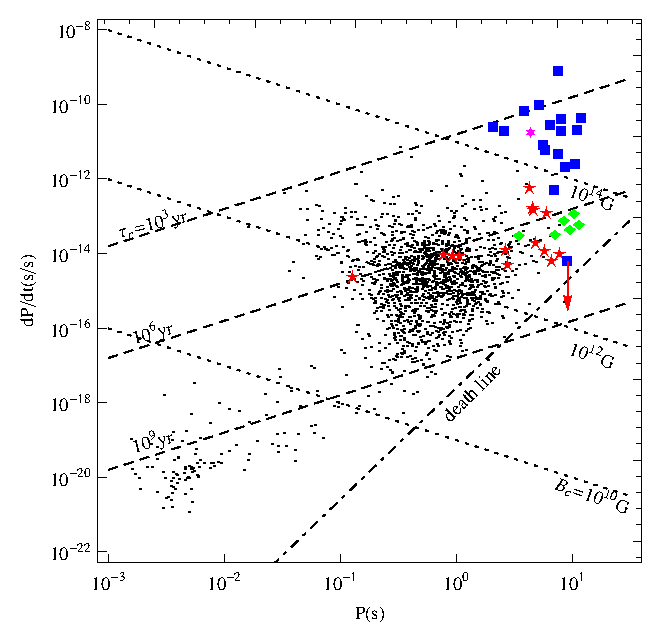
\includegraphics[width=12cm]{PPdot.eps}
\caption{脉冲星的P-$\mathrm{\dot{P}}$图\supercite{tx11}。方形点代表反常X射线脉冲星和
软伽马射线重复爆,六角星代表射电噪的磁星,向下的箭头代表低磁场的
软伽马射线重复爆(数据来自McGill online catalog:
http://www.physics.mcgill.ca/$\sim$pulsar/magnetar/main.html)。
菱形代表X射线暗的孤立中子星(X-ray dim isolated neutron stars,XDINSs)
(数据来自Kaplan \& van Kerkwijk (2011)\supercite{kv11})。星形代表转
动射电暂现源(rotating radio transients,RRATs), 点代表常规脉冲星
和毫秒脉冲星(数据来自ATNF: http://www.atnf.csiro.au/research/pulsar/psrcat/)。}
\label{PPdot}
\end{figure}

反常X射线脉冲星和软伽马射线重复爆的自转周期分布在一个比较窄的范围内,$2-12$\,s,
并且自转周期的导数与射电脉冲星比起来比较大(见图\ref{PPdot})。但是我们也发现了
自转周期导数比较小的软伽马射线重复爆SGR 0418$+$5729\supercite{ret10}。
%
反常X射线脉冲星的测时噪声远大于射电脉冲星,而软伽马射线脉冲星的测时噪声甚至
更大。我们在所有有长时间测时数据的反常X射线脉冲星中都观测到了跳变现象(glithes)。
大多数反正X射线脉冲星的跳变现象和年轻射电脉冲星的相似,这暗示反常X射线脉冲星和
软伽马射线重复爆是比较年轻的脉冲星。然而,他们的跳变的幅度比有相似自转周期的射电
脉冲星更大,发生的频率也更高。跳变的起源仍然不清楚,但是所观测到的各种现象似乎
跟反常X射线脉冲星和软伽马射线重复爆的星震模型更加符合\supercite{m08}。
%
另外一个有趣的发现是在软伽马射线重复爆的巨爆发的尾巴中的准周期振荡(quasi 
periodic oscillations,QPOs)现象。这个现象最初是被RXTE卫星在SGR 1806$-$20在
2004年12月27日的巨爆发的尾巴中发现的\supercite{ibs05},并且被RHESSI卫星
独立地确认\supercite{ws06}。在RXTE的SGR 1900$+$14在1998年八月的巨爆发的数据
中也发现了准周期振荡现象\supercite{sw05}。这种在巨爆发的尾巴中发现的准周期振荡
现象很可能源自于由剧烈的爆发导致的星体壳层的碎裂和震动,与地球的地震相似\supercite{m08}。

\subsection{磁星模型和“夸克星+回落盘”模型}

反常X射线脉冲星和软伽马射线重复爆的研究中的一个最根本的问题是,持续X射线辐射
和爆发现象的能源机制。反常X射线脉冲星和软伽马射线重复爆的爆发现象的能量达到
$10^{42}$\,$\rm{erg\ s^{-1}}$的量级,远大于自转所能提供的能量。一种可能的解释
是,孤立中子星是有磁场供能的,这种模型叫做磁星模型。在磁星模型下,反常X射线
脉冲星和软伽马射线重复爆都是由极强的磁场供能的,磁场强度达到$3\times10^{17}\times(1\ \rm{ms}/P_{\rm{0}})$。
这样的极强磁场是由非常高效的发电机机制产生的,并且假设中子星在诞生时的自转
周期足够短($P_{\rm{0}}\sim1-2$\,ms),同时还有对流的存在\supercite{td93}。
由于很强的偶极辐射,磁星的自转减慢非常大,而很窄的自转周期的分布则解释为
年轻的磁星很快的自转减慢到几秒,然后快速演化到“死亡线”以下。随着自转减慢,
磁场能量,$E_{\rm{mag}}\sim10^{46}(P/5\ \rm{s})(\dot P/10^{-11}\ \rm{s\ s^{-1}})$ ergs,
很快超过自转能损\supercite{m08}。磁场的衰减提供了巨大的内部的加热,从而
产生持续的X射线辐射。而爆发现象则被解释为磁重连\supercite{td93}。

尽管磁星模型得到了深入的发展并且被广泛使用,但是随着观测的不断激烈越来越多的
问题被暴露出来。我们没有发现磁星模型预测的很大的kick速度\supercite{hcb+07}和
高能量的超新星\supercite{gsg+01,vk06},我们也没有观测到反常X射线脉冲星和软
伽马射线重复爆的伽马射线辐射\supercite{tsx11}。
%
因此,不同于磁星模型的解释是有必要的,并且很有希望可以更好地解释观测。
“夸克星+回落盘”就是一个能解释我们观测到的各种反常脉冲星和软伽马射线
重复爆的现象的模型。超新星爆发抛出的一些物质可能会回落到中子星周围,如果
这些回落物质带有角动量,那么它们将形成中子星周围的回落盘。反常X射线脉冲星
和软伽马射线重复爆的自转周期的分布可以解释为当共转半径等于磁层半径是达到
的回落盘的平衡周期,而回落盘的制动可以解释比射电脉冲星大的自转周期的减慢\supercite{a01,chn00}。
反常X射线脉冲星和软伽马射线重复爆的持续X射线辐射可以通过吸积过程产生,
而爆发现象则解释为夸克星的引力能、弹性能以及相变能的释放\supercite{tx11}。
夸克星还能解释超爱丁顿光度的爆发现象,因为夸克星是有强相互作用束缚的。

\subsection{反常X射线脉冲星和软伽马射线重复爆的硬X射线辐射}

反常X射线脉冲星和软伽马射线重复爆的硬X射线辐射的发现相较于软X射线
辐射是比较晚的。考虑到它们在10\,keV以下的比较软的谱,所发现的一直延伸
到150\,keV的硬X射线辐射让人比较惊讶\supercite{khm04,mcl+04,dhk+06}。
在软伽马射线重复爆的尾巴中硬X射线辐射也没发现了\supercite{mgm+05,gmt+06}。
到目前为止,20\,keV以上的硬X射线辐射已经在五颗反常X射线脉冲星
(4U 0142$+$61,1RXS J1708$-$40,1E 1048$-$59, 1E 1841$-$045,1E 1547$-$54)\supercite{dhk+06,khd+06,lwr08,khm04,enm+10}
以及两颗软伽马射线重复爆(SGR 1900$+$14, SGR 1806$-$20)\supercite{gmt+06,emt+07}
中发现。对于没有探测到硬X射线辐射的源,目前给出的上限也不足以排除硬
X射线辐射存在的可能性。反常X射线脉冲星在20\,keV以上的谱能用一个比较硬
的幂律谱拟合,而软伽马射线重复的硬X射线谱要更陡。更重要的是,在
X射线波段的比较硬的谱说明在这个波段释放的能量占了总能量的很大
一部分\supercite{m08}。

我们还不能很好地理解反常X射线脉冲星和软伽马射线重复爆的硬X射线辐射的
起源。一方面,目前的观测被硬X射线脉冲星较低的灵敏度限制。另一方面,
理论模型还有待发展。在磁星模型的框架下,人们提出了几种可能的辐射机制。
Thompson \& Beloborodov (2005)\supercite{tb05}给出了两种机制,一种
可能性是由星体表面的薄的湍流层产生的韧致辐射,另一种可能性是在星体
表面以上约100公里的高度产生的同步辐射。第一种可能性预言硬X射线谱在
几百keV会出现阶段,而第二种可能性则预言硬X射线辐射会一直延伸到1\,MeV
甚至更高能。Heyl \& Hernquist (2005)\supercite{hh05}根据fast-mode 
breakdown模型提出,硬X射线是由在磁层外部的非热的正负电子的回旋辐射
产生的。Baring and Harding (2007)\supercite{bh07}提出,共振回旋
散射(resonant cyclotron scattering,RCS)是产生硬X射线辐射的机制。
考虑到磁层中的等离子体的密度很高,同时磁场很强,康普顿散射会在
回旋能量产生共振,从而大大增加散射截面。由星体表面辐射出的热光子
被共振回旋散射到硬X射线的能量。这个模型预言一个很平的谱。
在回落盘的模型下,软X射线和硬X射线辐射都被解释为由吸积过程产生的。
幂律的硬X射线谱是在吸积流中由于整体康普顿化(bulk-motion Comptonization)
的光子产生的,而这些光子来自星体表面的热辐射。使用这一模型,
Tr\"{u}mper et al. (2010)\supercite{tze+10}成功地模拟了AXP 4U 0142$+$61
的软X射线和硬X射线谱。

\begin{figure}
\begin{center}
\includegraphics[width=2 in,angle=-90]{10ms_comptb_po.ps}
\includegraphics[width=2 in,angle=-90]{1ms_comptb_po.ps}
\caption{AXP 4U 0142+61的模拟硬X射线谱。左图曝光时间为$10^7$\,s,
右图曝光时间为$10^6$\,s。红色的点和线代表共振回旋辐射模型,黑
色的点和线代表整体康普顿化模型。}
\label{10ms}
\end{center}
\end{figure}

\begin{figure}
\centering
\includegraphics[height=0.45\textwidth, angle=-90]{1708spe.eps}
\includegraphics[height=0.45\textwidth, angle=-90]{1547spe.eps}\\
\includegraphics[height=0.45\textwidth, angle=-90]{1806spe.eps}
\includegraphics[height=0.45\textwidth, angle=-90]{0501spe.eps} \\
\caption{四颗反常X射线脉冲星/软伽马射线重复爆的$E^2f(E)$。最佳的整体康普顿化模型的拟合结果和
拟合的參差也分别给出。Suzaku XIS和INTEGRAL IBIS-ISGRI数据分别用黑线和红线表示。}
\label{bmc}
\end{figure}

尽管对于反常X射线脉冲星和软伽马射线重复爆的硬X射线辐射的研究
受限于目前的硬X射线望远镜的较低灵敏度,但是这种状况很快会随着
下一代望远镜,例如NuStar和硬X射线调制望远镜(Hard X-ray Modulation 
Telescope,HXMT),的运行而得到改变。硬X射线波段观测的灵敏度
的显著提高有望帮助我们区分不同的辐射模型,从而进一步理解反常X
射线脉冲星和软伽马射线重复爆的本质。我们通过模拟反常X射线脉冲星
和软伽马射线重复爆的硬X射线谱,研究了未来使用硬X射线调制望远镜
区分不同辐射模型的可能性。我们主要考虑了两种辐射模型,一种
是磁星模型下的共振回旋辐射机制,一种是回落盘模型下的整体康普顿
化机制。这两种辐射机制预言了非常不同的硬X射线谱。共振回旋辐射
预言了一个延伸到MeV的很平的谱,而整体康普顿散射模型则预言硬
X射线谱会在200\,keV附近截断。使用硬X射线调制望远镜的响应矩阵,
我们基于以上两种模型模拟了AXP 4U 0142+61的硬X射线能谱。我们
的模拟显示,未来硬X射线调制望远镜的观测很有希望区分这两种模型。
在图\ref{10ms}中,我们假设$10^7$\,s和$10^6$\,s的曝光时间模拟
了AXP 4U 0142+61的能谱。我们可以看到硬X射线调制望远镜在硬X射
线能短的高灵敏度能帮助我们清楚地区分两种不同的辐射模型。

除了进行模拟,我们也尝试使用现有的数据来检验回落盘模型框架
下整体康普顿化机制。Guo, \textbf{Dai}, Li et al. (2014)\supercite{gdl+14}
使用Suzaku和INTEGRAL卫星的数据研究了四个源的软X射线和硬X射线辐射
(1RXS J170849-400910,1E 1547.0-5408,SGR 1806-20,SGR 0501+4516)。
我们的结果显示,这四个源的软X射线和硬X射线谱能比较好的被整体
康普顿化模型拟合,说明回落盘模型是可以解释反常X射线脉冲星和
软伽马射线重复爆的X射线辐射的。

%\section{夸克星相变潜热作为伽玛射线暴余辉能量注入的研究}
%
%冷夸克物质的费米能远高于热能,主要的自由度是夸克自由度,它们的物态至今仍不能很好理解,
%这一方面是由于在低能下夸克之间的强相互作用的非微扰效应,另一方是由于多体问题的困难。
%中子星作为最致密的一种天体之一,其中心的密度高达几倍核物质密度,这无疑为我们提供了一个
%研究夸克物质物态的绝佳场所。有相对论重离子碰撞实验的证据显示,在热夸克胶子等离子体中,
%夸克间的相互作用很强\supercite{Shuryak09},那么自然地当温度降低时,夸克之间的相互作用
%可能更强。相对论性的夸克物质基态可能不是费米气\supercite{Xu09},于是夸克可能集团,
%而如果夸克团块之间的剩余强相互作用势能高于它们的动能,则夸克团块将被束缚在势垒中,
%形成固态夸克物质,我们推测天体物理中的冷夸克物质可能处于这样的固态\supercite{Xu03}。
%
%由于目前我们尚不能得到冷夸克物质的相对论性状态方程,通常只能使用一些唯象模型来描述,
%Lai \& Xu (2009)使用了~Lennard-Jones~势来讨论固态夸克星\supercite{Lai09},得到了夸
%克星的状态方程。基于Lai \& Xu (2009)的固态夸克星模型,我们可以尝试估算夸克星从液态
%相变到固态时放出的相变潜热以及相变温度,并将估算结果应用于伽玛暴余辉平台的解释。
%
%
%假设夸克星内部的单个夸克团块是不带色的,于是我们可以将夸克星内部的夸克团块与惰性气体
%中电中性的的惰性气体分子类比。我们知道惰性气体分子之间的相互作用能很好地用~Lennard-Jones~势来刻画:
%\begin{equation}
%u(r)=4U_{0}[(\frac{r_{0}}{r})^{12}-(\frac{r_{0}}{r})^{6}]
%\end{equation}
%其中,$U_{0}$ 是势井深度,$r_{0}$ 代表相互作用的范围。我们假设这样一个短程排斥,
%长程吸引的相互作用势也能描述夸克团块之间的相互作用,那么当夸克团块间的相互作用势井足
%够深,以至于能将夸克团块束缚于势垒内时,夸克物质就将固化,形成固态夸克物质。由于
%色相互作用远远强于电磁相互作用,$U_{0}$ 和 $r_{0}$ 两个参数在冷夸克物质中将会不同
%于惰性气体中,并且决定了固态夸克物质的状态。用~Lennard-Jones~势来刻画的固态夸克星模型
%完全不同于用~MIT bag model~等模型来刻画的夸克物质模型。相比于在传统模型中夸克物质
%的基态是费米气,在~Lennard-Jones~势所描述的固态夸克星模型中,夸克团块是非相对论性
%的粒子,并且预言了一个更硬的状态方程,意味着夸克星的最大质量将更大($>2M_{\odot}$)。
%
%基于用~Lennard-Jones~势来描述的固态夸克星模型,我们可以尝试估算夸克星由液态相变到
%固态的过程中放出的相变潜热及相变温度。这样的相变过程有可能发生在夸克星形成的初期,
%当夸克星由高温逐渐冷却时,例如我们将讨论的伽玛暴余辉阶段。在我们所考虑的固态夸克星
%模型下,夸克团块作为非相对论性粒子,由之间的类似于~Lennard-Jones~势的剩余色相互作用
%束缚在一起,与惰性气体非常相似,与常见的物质也有很多相似之处。鉴于我们很难从分子动
%力学的方法直接出发,模拟夸克物质从液态相变到固态的过程,并得到相变潜热和相变温度,
%我们考虑通过与惰性气体,以及常规物质的类比,尤其是参考各种物质的相变潜热和
%相互作用强度的数据,从量级上估算夸克星由液态相变到固态时释放的相变潜热,这对于我们
%讨论伽玛暴余辉的能量注入是十分有意义的。在表\ref{heat}中,我们列出了一些常见物质
%和惰性气体的熔解热,气化热,势能以及势能与熔解热之比的实验数值,其中熔解热正对应于
%从液态相变到固态的相变潜热,而势能的数值对于有升华热数据的物质就是升华热,对于没
%有升华热数据的物质则是熔解热和气化热之和。我们看到,对于大部分物质,包括惰性气体,
%势能与熔解热之比在几十到一百之间,特例是氦的比值较高,这可能与氦复杂的物态有关。考
%虑到夸克团块间的相互作用与惰性气体相似,且夸克团块的质量不大,我们取势能与熔解热之比
%为$20\sim100$进行估算。而在之前讨论的固态夸克星模型下,取势井深度$U_{0}=100$\,MeV,
%那么我们可以估算得到单个夸克团块由液态相变到固态是放出的相变潜热为$1\sim5$\,MeV。假
%设夸克星的质量是一个太阳质量,$M_{\odot}\approx2\times10^{33}$\,g,约包含重子数目为
%$10^{57}$个,这样我们得到一个太阳质量的夸克星由液态相变到固态放出的相变潜热约为$E\approx10^{51}$\,ergs,
%这个估算值基本上就是伽玛暴余辉释放能量的典型值,也就是说夸克星由液态相变到固态时释
%放的相变潜热完全足够提供伽玛暴余辉平台需要的能量注入。
%						
%\begin{table}[htb!]
%\caption{一些常见物质和惰性气体的熔解热,气化热,势能以及势能与熔解热之比}
%\label{heat}
%\centerline{\begin{tabular}{lccccc}\hline
%	&  熔解热 kcal/mol  & 气化热 kcal/mol   & 势能 kcal/mol  &   势能/熔解热  \\
%\hline
%$He$ & 0.0033 & 0.0194 & 2.2944   & 695.27 \\
%$Ne$ & 0.0801 & 0.422  & 9.1776   & 114.58 \\
%$Xe$ & 0.5495 & 3.02   & 12.6192  & 22.96  \\
%$Rn$ & 0.69   & 4.01   & 19.5024  & 28.26  \\
%&        &        &          &        \\
%$Al$ & 2.56   & 69.5   & 78       & 30.47  \\
%$Cs$ & 0.499  & 16.198 & 18.3     & 36.67  \\
%$Cu$ & 3.17   & 72.74  & 81       & 25.55  \\
%$Fe$ & 3.63   & 83.68  & 99.5     & 27.41  \\
%$Hg$ & 0.5486 & 14.13  & 14.65    & 26.7   \\
%$Na$ & 0.622  & 23.285 & 25.75    & 41.4   \\
%$Si$ & 12     & 85.8   & 107.7    & 8.98   \\
%$C$  & 25     &        & 171.29   & 6.85   \\
%$CO$ & 0.2    & 1.444  & 1.644    & 8.22   \\
%$CO_{2}$  & 1.99      &        & 6.03   & 3.03  \\
%$H_{2}O$  & 1.436      &  9.717    & 11.153   & 7.77  \\
%$H_{2}O_{2}$  & 2.987   &  10.53   & 12.34   & 4.13   \\
%$CaCl_{2}$  & 6.8      & 56.2       & 77.5   & 11.4  \\
%\hline
%\end{tabular}}
%\end{table}
%
%另一方面,根据~Lindemann~经验定则,当固体中原子振动强度的方均根与平衡的相
%邻原子距离的比值大于一定的临界值时固体熔解\supercite{Lindemann10},我们可以
%估算夸克星相变的温度。~P. Mohazzabi~和~F. Behroozi~在~1987~年的工作中得到,
%对于惰性气体,原子振动强度的方均根与平衡的相邻原子距离的比值有表达式:
%\begin{equation}
%\frac{\langle u^{2} \rangle}{R_{0}^{2}}=\frac{\varepsilon_{0}/kT}{4(\exp(-\alpha/kT)-\exp(-\varepsilon_{0}/kT))}\int_{\alpha/\varepsilon_{0}}^{1}[(1-x^{1/2})^{-1/6}-(1+x^{1/2})^{-1/6}]^{2}\exp(-\varepsilon_{0}x/kT)/\rm{d}x
%\end{equation}
%其中$x=1+(\varepsilon/\varepsilon_{0})$,$\varepsilon_{0}=U_{0}S_{6}^{2}/6S_{12}$,
%$k$是玻尔兹曼常数,对于简单的面心立方晶体,$S_{6}=14.45392$,
%$S_{12}=12.13188$\supercite{Moha87},带入惰性气体的参数后发现比值很好地与
%经验定则符合。对于我们的估算,可以直接参考惰性气体以及普通物质的势能与
%热能的比值,$\Gamma=U_{0}/kT$,从而估算夸克星相变的温度。表\ref{temp}列出了
%惰性气体的相关参数,可以发现,势能与热能的比值大约在$1.75$左右。而对于其他
%物质,例如对于单一组分的等离子体,液体固化时库伦势与热能的比值是$\Gamma\approx175$\supercite{DeWitt01},
%对于混合组分的等离子体,$\Gamma\approx233$\supercite{Horowitz07}。因此,
%若取势井深度$U_{0}=100$\,MeV,我们可以直接估算得到夸克星的相变温度大约在$1\sim10$\,MeV。
%\begin{table}[htb!]
%\caption{惰性气体的相变温度和势能}
%\label{temp}
%\centerline{\begin{tabular}{lccc}\hline
%	&  熔点 K  & $U_{0}/\rm{k}$ K   & $U_{0}/\rm{k}T$  \\
%\hline
%$Ne$ & 24.5 & 45.86  & 1.87 \\
%$Ar$ & 83.8 & 142.095   & 1.70  \\
%$Kr$ & 115.8   & 201.9   & 1.74  \\
%$Xe$ & 161.4   & 281.0   & 1.74  \\
%\hline
%\end{tabular}}
%\end{table}
%
%处在液态到固态相变过程中的夸克星将保持稳定的相变温度,同时向外辐射相变
%潜热,我们假设夸克星的热辐射是一个灰体辐射,辐射效率是$\eta\ll1$,则我
%们可以估算夸克星辐射相变潜热的时标:
%\begin{equation}
%t=\frac{E}{\sigma T^{4} 4\pi R^{2}\eta}
%\end{equation}
%其中,$E=10^{51}$\,ergs,$\sigma$是~Stefan-Boltzman~常数,$R=10$\,km
%是夸克星的半径,考虑到$\eta\ll1$,带入$T\approx1$\,MeV计算可得,相变潜
%热的辐射时标$t\approx1000$\,s,这是与伽玛暴余辉的平台持续时间基本一致的。
%
%在估算了夸克星由液态相变到固态时放出的相变潜热,以及能量注入的时标之后,
%我们有必要定性地讨论一下相变潜热以怎样的方式注入伽玛暴余辉的问题。
%夸克星由液态到固态的相变过程应该发生在伽玛暴的爆发阶段之后,具体的时标依赖于夸克星形成之后的冷却过
%程,但我们可以预期,相变发生时,伽玛暴的爆发过程已经结束,原始火球已经膨胀到了很远的距离,或者已经进
%入外部介质,在夸克星表面到火球内边界或外部介质内边界之间形成了一个“真空”。由于原始火球已经将这个空间
%内的大部分重子物质带出,我们假设这个空间里的重子物质密度很低,只有原始密度的$1\% \sim 0.1\%$。
%根据我们的估算结果,夸克星相变释放的相变潜热约为$E=10^{51}$\,ergs,以灰体辐射的方式释放能量的时间约
%为$1000$\,s,于是我们可以估算得到,能流约为$L=10^{48}$\,ergs/s,相比于爆发阶段的能流小了三个量
%级,然而如果用夸克星半径$R=10$\,km 作为源的尺度来估算光深,我们可以得到:
%\begin{equation}
%\tau_{\gamma\gamma}=\frac{f_{p}\sigma_{T}FD^{2}}{R^{2}m_{e}c^{2}}=10^{13}f_{p}(\frac{D}{3000\rm{Mpc}})^{2}(\frac{F}{10^{-11}\rm{ergs/cm^{2}}})(\frac{R}{10\rm{km}})^{-2}
%\end{equation}
%可见光深仍然非常大。因此,由夸克星相变释放出的相变潜热能流仍将类似于原始火球,
%是由光子,电子对和少量重子物质构成的类似理想流体的等离子体,并且在内部压强的作
%用下加速膨胀,不同的是火球不再是以极端相对性速度朝静止观测者运动,同时由于相变
%过程相对稳定,也不会在火球内产生壳层。这样的一个由释放相变潜热形成的火球将基本
%按照我们在上一节中讨论的火球演化的过程演化,也会有由光厚到光薄的过度,以及有
%辐射主导到物质主导的过度。然而无论演化过程怎么样,我们期待最后能量将转化为
%重子物质的动能,于是我们可以简单地估算最后由重子物质主导的火球的速度:
%\begin{equation}
%\gamma=L/Mc^{2}
%\end{equation}
%我们知道在爆发阶段,$\gamma\approx100$,而如前所述,我们考虑夸克星相变潜热注
%入阶段,能流比爆发阶段小三个数量级,而重子物质质量为原始质量的 $1\%$,由此可得
%$\gamma\approx10$。而这样的相对能量密度较小的能流,以 $\gamma\approx10$的速度
%进入外部介质,根据Zhang et al. (2002)\supercite{Zhang02},能流将以类似于~Poynting~
%流的方式注入余辉。
%
%由以上的论述,我们可以大致描绘夸克星相变潜热注入伽玛暴余辉的图像,在伽玛暴的爆
%发阶段结束以后,中心形成的夸克星温度逐渐降低,当达到固化温度时,夸克星发生由液态
%向固态的相变,相变过程中温度稳定在相变温度,相变潜热则以灰体辐射的方式稳定地向外辐射;
%辐射出的光子由于能量密度很高,光深很大,产生大量电子对,而光子,电子对和少量的重子
%物质耦合在一起类似理想流体,按照爆发阶段火球演化相类似的方式演化;随着火球的膨胀,
%最终能量将基本上转化为重子物质的动能,而由于潜热释放的能流较小,虽然重子物质相较
%于爆发阶段少很多,最后加速达到的速度也不是很高,而这样的能流较小,速度不高的火球
%将以类似于~Poynting~流的形式注入余辉,也就是说将能量较平和地转换给外部介质的物质,
%从而产生余辉阶段的平台;而在相变结束之后,相变潜热的注入停止,外部介质不再得到
%能量注入,辐射的流量迅速降低,从而产生光变曲线平台后的快速而陡峭的下降。

\pkuthssffaq


	% 结论。
	% vim:ts=4:sw=4
% Copyright (c) 2014 Casper Ti. Vector
% Public domain.

\specialchap{结论}

我针对脉冲星类致密天体展开了多波段的研究,积累了多波段的观测、
数据处理和分析的经验。未来的脉冲星研究必将是联合多波段的观测进行的,
而未来多个地面和空间的、跨越多个波段的天文望远镜将有希望为我们
解开脉冲星类致密天体的本质的谜团,同时使我们可以通过脉冲星测时
探测和研究引力波辐射。

我在博士期间的工作可以总结如下:
\begin{itemize}
\item 射电波段的研究:

\begin{enumerate}
\item 我们研究了24颗毫秒脉冲星的多波段偏振脉冲轮廓。长达六年的PPTA数据
使我们可以在三个波段上给出高信噪比的偏振脉冲轮廓,从而能够研究单个脉冲成分以及
它们如何随频率演化,并发现了之前没有发现过的脉冲轮廓特征。对于我们的
样本中的多颗脉冲星,脉冲辐射几乎覆盖了整个脉冲周期。脉冲成分的宽度和脉冲
成分的间隔随频率的演化很复杂,一些情况下这些量随着频率的升高而增大,另一些
情况下则减小。偏振特性随频率的演化也极为复杂。我们发现脉冲轮廓的前导成分
和尾部成分相比主脉冲成分有更高的线偏振度。我们使用三个频率的观测测量了
这些脉冲星的谱指数和法拉第旋转。对于大部分脉冲星,它们的谱符合幂率谱,而
偏振位置角也符合$\lambda^2$的关系。但是也有一部分脉冲星明显偏离这些关系。
我们还给出了每颗脉冲星的相位分离谱指数、线偏振度和法拉第旋转。我们发现
这些量在整个脉冲周期上有系统的变化,并与脉冲轮廓的结构有关。
\item 我们研究了多种与频率相关的效应对高精度脉冲星测时的影响,特别是对于
宽波段的接收机系统的影响。这些效应包括星际闪烁效应、色散延迟效应、脉冲轮廓随频
率的演化以及多普勒效应。我们开发了脉冲星观测的模拟软件,可以模拟星际闪烁
以及脉冲轮廓的演化。通过模拟,我们展示了这些效应对现有的数据以及未来的
宽波段观测的影响。为了消除这些效应,我们开发了新的脉冲星测时软件,进行
频率相关的测时,并且在测量脉冲到达时间的同时测量色散延迟。
\item 我们讨论了FAST在未来的PTA研究中扮演的角色。PTA的主要科学目标是探测
超低频的引力波、建立脉冲星时间标准以及改进太阳系的行星历书。而FAST将
发现大量新的毫秒脉冲星,并且大大地提高脉冲星测时的精度,因此将在未来的PTA研究中
扮演重要的角色。然而,在几年的时标上,FAST的脉冲星测时将受到
jitter noise的限制,而在更长的时标上脉冲星测时噪声将变得很重要。

\end{enumerate}

\item 光学波段的研究:

我们研究了银河系中由中子星和射电脉冲星导致的微引力透镜事件的性质。对于一个全天的
photometric microlensing巡天并假设可以监测10$^{10}$颗背景天体,我们的估算显示由约
120000颗可观测的射电脉冲星导致的事件率为0.2\,yr$^{-1}$。考虑到astrometric 
microlensing的截面更大,因此我们期待对于一个astrometric microlensing的巡天,假设
相同的背景天体和可观测脉冲星数目,每年我们可以发现几个事件。
%
我们的计算显示,对于由中子星导致的银河系photometric microlensing事件,持续的时标比
之前的人们的估算短,这主要是由于中子星比较大的自行。在银河系中心方向,对于时标约为
15天的photometric microlensing事件,约有7\%是由中子星导致的。对于更长时标的事件,这
个比例快速下降。在远离银河系中心的方向上,对于时标短于10天的事件,中子星贡献的比例
可以高达40\%。这些结果是与之前的没有考虑中子星分布的工作不同的,他们预测中子星将
主要导致长时标的微引力透镜事件。
%
考虑到未来的望远镜很可能发现由射电脉冲星导致的astrometric microlensing事件,我们研究了
通过这些事件测量脉冲星质量的精度。我们的计算显示,astrometric microlensing现象可以帮助
我们较准确地测量脉冲星的质量。如果脉冲星的距离可以通过射电观测独立测量,那么脉冲星的
质量可以被测量精确到约10\%。

\item X射线波段的研究:

多颗反常X射电脉冲星和软伽马射线重复爆在10\,keV以上的硬X射线被探测到,但是目前仍不能理解
这些硬X射线辐射的起源。人们提出了多种模型来解释反常X射线脉冲星和软伽马射线重复爆的硬X射线
辐射的起源和物理机制,这些模型基于不同的对于这一类天体本质的理解,包括磁星模型和回落盘
系统模型。我们使用Suzaku和INTEGRAL卫星的数据研究了两颗反常X射线脉冲星
(1RXS J170849‑400910,1E 1547.0‑5408)和两颗软伽马射线重复爆
(SGR 1806‑20,SGR 0501+4516)的软X射线和硬X射线辐射。
我们发现它们在软X射线和硬X射线波段辐射能被整体康普顿化模型统一地
拟合(bulk-motion Comptonization)。
这说明在回落盘系统的模型下,反常X射线脉冲星和软伽马射线重复爆的X射线辐射可以被解释的。
根据不同的模型对硬X射线谱的预言,我们进一步对未来HXMT的观测进行了模拟。我们的模拟显示,
未来HXMT的观测很有希望帮助我们区分不同的辐射模型,从而帮助我们理解反常X射线脉冲星和软伽
马射线重复爆的本质。

\end{itemize}
\pkuthssffaq



	% 正文中的附录部分。
	\appendix
	% 排版参考文献列表。
	\printbibliography[
		% 使“参考文献”出现在目录中;如果同时要使参考文献列表参与章节编号,
		% 可将“bibintoc”改为“bibnumbered”。
		heading = bibintoc,
		% 单独设定排序方案。此设定会局部覆盖之前的全局设置。
		% 注:只有同时使用 2.x 或之后版本的 biblatex 和相应兼容版本的 biber,
		% 才能对每个 \printbibliography 命令采用不同的排序方案,
		% 否则只能在导入 biblatex 宏包时就(全局)指定排序方案。
		% 在这样的情况下,请去掉所有的 sorting 选项,否则可能出错。
		sorting = ecnty
	]
	% 各附录。
	% vim:ts=4:sw=4
% Copyright (c) 2014 Casper Ti. Vector
% Public domain.

\chapter{毫秒脉冲星的多波段脉冲偏振轮廓图片}

\begin{figure*}
\begin{center}
\includegraphics[width=6 in]{0437.ps}
\caption{PSR J0437$-$4715的多波段偏振轮廓和相位分离研究.}
\label{0437}
\end{center}
\end{figure*}

\begin{figure*}
\begin{center}
\includegraphics[width=6 in]{0613.ps}
\caption{PSR J0613$-$0200的多波段偏振轮廓和相位分离研究.}
\label{0613}
\end{center}
\end{figure*}

\begin{figure*}
\begin{center}
\includegraphics[width=6 in]{0711.ps}
\caption{PSR J0711$-$6830的多波段偏振轮廓和相位分离研究.}
\label{0711}
\end{center}
\end{figure*}

\begin{figure*}
\begin{center}
\includegraphics[width=6 in]{1017.ps}
\caption{PSR J1017$-$7156的多波段偏振轮廓和相位分离研究.}
\label{1017}
\end{center}
\end{figure*}

\begin{figure*}
\begin{center}
\includegraphics[width=6 in]{1022.ps}
\caption{PSR J1022$+$1001的多波段偏振轮廓和相位分离研究.}
\label{1022}
\end{center}
\end{figure*}

\begin{figure*}
\begin{center}
\includegraphics[width=6 in]{1024.ps}
\caption{PSR J1024$-$0719的多波段偏振轮廓和相位分离研究.}
\label{1024}
\end{center}
\end{figure*}

\begin{figure*}
\begin{center}
\includegraphics[width=6 in]{1045.ps}
\caption{PSR J1045$-$4509的多波段偏振轮廓和相位分离研究.}
\label{1045}
\end{center}
\end{figure*}

\begin{figure*}
\begin{center}
\includegraphics[width=6 in]{1446.ps}
\caption{PSR J1446$-$4701的多波段偏振轮廓和相位分离研究.}
\label{1446}
\end{center}
\end{figure*}

\begin{figure*}
\begin{center}
\includegraphics[width=6 in]{1545.ps}
\caption{PSR J1545$-$4550的多波段偏振轮廓和相位分离研究.}
\label{1545}
\end{center}
\end{figure*}

\begin{figure*}
\begin{center}
\includegraphics[width=6 in]{1600.ps}
\caption{PSR J1600$-$3053的多波段偏振轮廓和相位分离研究.}
\label{1600}
\end{center}
\end{figure*}

\begin{figure*}
\begin{center}
\includegraphics[width=6 in]{1603.ps}
\caption{PSR J1603$-$7202的多波段偏振轮廓和相位分离研究.}
\label{1603}
\end{center}
\end{figure*}

\begin{figure*}
\begin{center}
\includegraphics[width=6 in]{1643.ps}
\caption{PSR J1643$-$1224的多波段偏振轮廓和相位分离研究.}
\label{1643}
\end{center}
\end{figure*}

\begin{figure*}
\begin{center}
\includegraphics[width=6 in]{1713.ps}
\caption{PSR J1713$+$0747的多波段偏振轮廓和相位分离研究.}
\label{1713}
\end{center}
\end{figure*}

\begin{figure*}
\begin{center}
\includegraphics[width=6 in]{1730.ps}
\caption{PSR J1730$-$2304的多波段偏振轮廓和相位分离研究.}
\label{1730}
\end{center}
\end{figure*}

\begin{figure*}
\begin{center}
\includegraphics[width=6 in]{1744.ps}
\caption{PSR J1744$-$1134的多波段偏振轮廓和相位分离研究.}
\label{1744}
\end{center}
\end{figure*}

\begin{figure*}
\begin{center}
\includegraphics[width=6 in]{1824.ps}
\caption{PSR J1824$-$2452的多波段偏振轮廓和相位分离研究.}
\label{1824}
\end{center}
\end{figure*}

\begin{figure*}
\begin{center}
\includegraphics[width=6 in]{1832.ps}
\caption{PSR J1832$-$0836的多波段偏振轮廓和相位分离研究.}
\label{1832}
\end{center}
\end{figure*}

\begin{figure*}
\begin{center}
\includegraphics[width=6 in]{1857.ps}
\caption{PSR J1857$+$0943的多波段偏振轮廓和相位分离研究.}
\label{1857}
\end{center}
\end{figure*}

%\clearpage

\begin{figure*}
\begin{center}
\includegraphics[width=6 in]{1909.ps}
\caption{PSR J1909$-$3744的多波段偏振轮廓和相位分离研究.}
\label{1909}
\end{center}
\end{figure*}

\begin{figure*}
\begin{center}
\includegraphics[width=6 in]{1939.ps}
\caption{PSR J1939$+$2134的多波段偏振轮廓和相位分离研究.}
\label{1939}
\end{center}
\end{figure*}

\begin{figure*}
\begin{center}
\includegraphics[width=6 in]{2124.ps}
\caption{PSR J2124$-$3358的多波段偏振轮廓和相位分离研究.}
\label{2124}
\end{center}
\end{figure*}

\begin{figure*}
\begin{center}
\includegraphics[width=6 in]{2129.ps}
\caption{PSR J2129$-$5721的多波段偏振轮廓和相位分离研究.}
\label{2129}
\end{center}
\end{figure*}

\begin{figure*}
\begin{center}
\includegraphics[width=6 in]{2145.ps}
\caption{PSR J2145$-$0750的多波段偏振轮廓和相位分离研究.}
\label{2145}
\end{center}
\end{figure*}

\begin{figure*}
\begin{center}
\includegraphics[width=6 in]{2241.ps}
\caption{PSR J2241$-$5236的多波段偏振轮廓和相位分离研究.}
\label{2241}
\end{center}
\end{figure*}

\pkuthssffaq


	% vim:ts=4:sw=4
% Copyright (c) 2014 Casper Ti. Vector
% Public domain.

\chapter{发表文章列表}

\begin{enumerate}
\item R. M. Shannon and 22 co-authors including \textbf{S. Dai},
``Gravitational waves from binary supermassive black holes missing in pulsar observations", 
\textsl{Science}, submitted.

\item \textbf{S. Dai}, G. Hobbs, R. N. Manchester, \textsl{et al}.
``A Study of Multi-frequency Polarization Pulse Profiles of Millisecond Pulsars",
\textsl{MNRAS}, 2015, 449, 3223.
			    
\item \textbf{S. Dai}, M. C. Smith, M. X. Lin, Y. L. Yue, G. Hobbs, R. X. Xu,
``Gravitational Microlensing of Neutron Star and Radio Pulsars: Event Rates, Time-scale Distributions and Mass Measurements",
\textsl{ApJ}, 2015, 802, 120.

\item J. B. Wang and 19 co-authors including \textbf{S. Dai},
``Searching for Gravitational Wave Memory Bursts with the Parkes Pulsar Timing Array", 
\textsl{MNRAS}, 2015, 446, 1657.

\item G. J. Guo, \textbf{S. Dai}, Z. S. Li, \textsl{et al}.
``To Understand the X-ray Spectrum of Anomalous X-ray Pulsars and Soft Gamma-ray Repeaters",
\textsl{RAA}, 2015, 15, 525.

\item Z. J. Qu, Z. S. Li, Y. P. Chen, \textbf{S. Dai}, L. Ji, R. X. Xu, S. Zhang,
``Analysis of Short Bursts in SGR 1806-20, 1E 1048-5937 and SGR 0501+4516",
\textsl{PASA}, 2015, 127, 211.

\item G. Hobbs, \textbf{S. Dai}, R. N. Manchester, R. M. Shannon, M. Kerr, K. J. Lee, R. X. Xu,
``The Role of FAST in Pulsar Timing Arrays",
\textsl{RAA, a special issue on FAST}, 2014, accepted, arXiv:1407.0435

\item X. J. Zhu and 18 co-authors including \textbf{S. Dai},
``An All-sky Search for Continuous Gravitational Waves in the Parkes Pulsar Timing Array Data Set", 
\textsl{MNRAS}, 2014, 444, 3709.

\item R. M. Shannon, S. Os{\l}owski, \textbf{S. Dai}, \textsl{et al}.
``Limitations in Timing Precision due to Single-pulse Shape Variability in Millisecond Pulsars",
\textsl{MNRAS}, 2014, 443, 1463.

\item T. Dolch and 42 co-authors including \textbf{S. Dai},
``A 24 Hr Global Campaign to Assess Precision Timing of the Millisecond Pulsar J1713+0747", 
\textsl{ApJ}, 2014, 794, 21.

\item \textbf{S. Dai}, L. X. Li and R. X. Xu,
``The Plateau of Gamma-ray Burst: Hint for the Solidification of Quark Matter?'',
\textsl{Science China G: Physics, Mechanics \& Astronomy}, 2011, 54, 1541.

\item \textbf{S. Dai}, R. X. Xu and A. Esamdin,
``Microlensing Pulsars'',
\textsl{MNRAS}, 2010, 405, 2754.

\end{enumerate}

\pkuthssffaq



	% 以下为正文之后的部分。
	\backmatter

	% 致谢。
	% vim:ts=4:sw=4
% Copyright (c) 2014 Casper Ti. Vector
% Public domain.

\chapter{致谢}

感谢国家和北京大学对我的培养、引导、宽容和关怀。感谢爸爸、妈妈和家人对我长久以来的爱和支持。
感谢我的导师徐仁新教授,教导我做人、治学。感谢George Hobbs博士作为导师和朋友给予我的帮助,让我在澳大利亚度过了非常精彩的十九个月。感谢Martin C. Smith博士对我的指导和帮助。

感谢北京大学物理学院和天文系为我提供的优越的学习条件,感谢这里的各位老师:乔国俊老师、吴鑫基老师、李柯枷师兄、黎卓老师、李立新老师、吴月芳老师、吴学兵老师、范祖辉老师、刘富坤老师、刘晓为老师、张华伟老师、张坚老师对我的指导,还有负责系务工作的姚洁老师所给予的帮助。感谢我的师兄师姐,感谢岳有岭、崔晓红、来小禹、于萌、那学森、庾君伟、刘雄伟对我的照顾和帮助。感谢我的同学张从尧、刘项琨、李彪、向茂盛、刘贝贝、郑晓晨、李程远和我一起度过这段难忘的燕园时光。

感谢CSIRO Astronomy and Space Science给我提供的联合培养的机会,感谢R. N. Manchester、S. Johnston、R. M. Shannon、M. Kerr、W. van Straten、W. A. Coles、L. Toomey、N. D. R. Bhat、J. M. Sarkissian、V. Drazenovic、N. Popo以及王洪光老师、游宵鹏老师给予我的帮助以及很多很多的讨论。感谢我在澳大利亚结识的朋友们,F. Cavallaro、T. Day、L. Gomez、A. Herzog、M. Karouzos、C. Ng、E. Servajean、C. Tiburzi陪伴我度过美好的时光。

感谢汪震陪伴我一路走过来,这篇论文献给我们的青春时光。
\pkuthssffaq


	% 原创性声明和使用授权说明。
	% vim:ts=4:sw=4
%
% Copyright (c) 2008-2009 solvethis
% Copyright (c) 2010-2014 Casper Ti. Vector
% All rights reserved.
%
% Redistribution and use in source and binary forms, with or without
% modification, are permitted provided that the following conditions are
% met:
%
% * Redistributions of source code must retain the above copyright notice,
%   this list of conditions and the following disclaimer.
% * Redistributions in binary form must reproduce the above copyright
%   notice, this list of conditions and the following disclaimer in the
%   documentation and/or other materials provided with the distribution.
% * Neither the name of Peking University nor the names of its contributors
%   may be used to endorse or promote products derived from this software
%   without specific prior written permission.
%
% THIS SOFTWARE IS PROVIDED BY THE COPYRIGHT HOLDERS AND CONTRIBUTORS "AS
% IS" AND ANY EXPRESS OR IMPLIED WARRANTIES, INCLUDING, BUT NOT LIMITED TO,
% THE IMPLIED WARRANTIES OF MERCHANTABILITY AND FITNESS FOR A PARTICULAR
% PURPOSE ARE DISCLAIMED. IN NO EVENT SHALL THE COPYRIGHT HOLDER OR
% CONTRIBUTORS BE LIABLE FOR ANY DIRECT, INDIRECT, INCIDENTAL, SPECIAL,
% EXEMPLARY, OR CONSEQUENTIAL DAMAGES (INCLUDING, BUT NOT LIMITED TO,
% PROCUREMENT OF SUBSTITUTE GOODS OR SERVICES; LOSS OF USE, DATA, OR
% PROFITS; OR BUSINESS INTERRUPTION) HOWEVER CAUSED AND ON ANY THEORY OF
% LIABILITY, WHETHER IN CONTRACT, STRICT LIABILITY, OR TORT (INCLUDING
% NEGLIGENCE OR OTHERWISE) ARISING IN ANY WAY OUT OF THE USE OF THIS
% SOFTWARE, EVEN IF ADVISED OF THE POSSIBILITY OF SUCH DAMAGE.

% 原创性声明和使用授权说明页不需要装订到论文中,故不显示页码。
\cleardoublepage\thispagestyle{empty}
\newgeometry{height = 240mm, width = 150mm, ignoreheadfoot, vcentering}
{
	\vspace*{\fill}\linespread{1.5}\selectfont
	\centerline{\bfseries\Large 北京大学学位论文原创性声明和使用授权说明}

	\vskip 4em
	\centerline{\bfseries\Large 原创性声明}
	\vskip 1em

	本人郑重声明:
	所呈交的学位论文,是本人在导师的指导下,独立进行研究工作所取得的成果。
	除文中已经注明引用的内容外,
	本论文不含任何其他个人或集体已经发表或撰写过的作品或成果。
	对本文的研究做出重要贡献的个人和集体,均已在文中以明确方式标明。
	本声明的法律结果由本人承担。
	\vskip 1em
	\rightline
	{%
		论文作者签名:\hspace{5em}%
		日期:\hspace{2em}年\hspace{2em}月\hspace{2em}日%
	}

	\vskip 4em
	\centerline{\bfseries\Large 学位论文使用授权说明}
	\centerline{\zihao{-4}(必须装订在提交学校图书馆的印刷本)}
	\vskip 1em

	本人完全了解北京大学关于收集、保存、使用学位论文的规定,即:
	\begin{itemize}
		\item 按照学校要求提交学位论文的印刷本和电子版本;
		\item 学校有权保存学位论文的印刷本和电子版,
			并提供目录检索与阅览服务,在校园网上提供服务;
		\item 学校可以采用影印、缩印、数字化或其它复制手段保存论文;
		\item 因某种特殊原因需要延迟发布学位论文电子版,
			授权学校在 $\square$\nobreakspace{}一年 / %
			$\square$\nobreakspace{}两年 / %
			$\square$\nobreakspace{}三年以后在校园网上全文发布。
	\end{itemize}
	\par(保密论文在解密后遵守此规定)
	\vskip 1em
	\rightline
	{%
		论文作者签名:\hspace{5em}导师签名:\hspace{5em}%
		日期:\hspace{2em}年\hspace{2em}月\hspace{2em}日%
	}

	% 若需排版二维码,请将二维码图片重命名为“barcode”,
	% 转为合适的图片格式,并放在当前目录下,然后去掉下面 2 行的注释。
	%\vskip 4em \noindent
	%\includegraphics[height = 5em]{barcode}

	\vspace*{\fill}\par
}
\restoregeometry


\end{document}

